% Options for packages loaded elsewhere
\PassOptionsToPackage{unicode}{hyperref}
\PassOptionsToPackage{hyphens}{url}
%
\documentclass[
]{book}
\usepackage{lmodern}
\usepackage{amsmath}
\usepackage{ifxetex,ifluatex}
\ifnum 0\ifxetex 1\fi\ifluatex 1\fi=0 % if pdftex
  \usepackage[T1]{fontenc}
  \usepackage[utf8]{inputenc}
  \usepackage{textcomp} % provide euro and other symbols
  \usepackage{amssymb}
\else % if luatex or xetex
  \usepackage{unicode-math}
  \defaultfontfeatures{Scale=MatchLowercase}
  \defaultfontfeatures[\rmfamily]{Ligatures=TeX,Scale=1}
\fi
% Use upquote if available, for straight quotes in verbatim environments
\IfFileExists{upquote.sty}{\usepackage{upquote}}{}
\IfFileExists{microtype.sty}{% use microtype if available
  \usepackage[]{microtype}
  \UseMicrotypeSet[protrusion]{basicmath} % disable protrusion for tt fonts
}{}
\makeatletter
\@ifundefined{KOMAClassName}{% if non-KOMA class
  \IfFileExists{parskip.sty}{%
    \usepackage{parskip}
  }{% else
    \setlength{\parindent}{0pt}
    \setlength{\parskip}{6pt plus 2pt minus 1pt}}
}{% if KOMA class
  \KOMAoptions{parskip=half}}
\makeatother
\usepackage{xcolor}
\IfFileExists{xurl.sty}{\usepackage{xurl}}{} % add URL line breaks if available
\IfFileExists{bookmark.sty}{\usepackage{bookmark}}{\usepackage{hyperref}}
\hypersetup{
  pdftitle={Basic R},
  pdfauthor={Kálmán Abari},
  hidelinks,
  pdfcreator={LaTeX via pandoc}}
\urlstyle{same} % disable monospaced font for URLs
\usepackage{color}
\usepackage{fancyvrb}
\newcommand{\VerbBar}{|}
\newcommand{\VERB}{\Verb[commandchars=\\\{\}]}
\DefineVerbatimEnvironment{Highlighting}{Verbatim}{commandchars=\\\{\}}
% Add ',fontsize=\small' for more characters per line
\usepackage{framed}
\definecolor{shadecolor}{RGB}{248,248,248}
\newenvironment{Shaded}{\begin{snugshade}}{\end{snugshade}}
\newcommand{\AlertTok}[1]{\textcolor[rgb]{0.94,0.16,0.16}{#1}}
\newcommand{\AnnotationTok}[1]{\textcolor[rgb]{0.56,0.35,0.01}{\textbf{\textit{#1}}}}
\newcommand{\AttributeTok}[1]{\textcolor[rgb]{0.77,0.63,0.00}{#1}}
\newcommand{\BaseNTok}[1]{\textcolor[rgb]{0.00,0.00,0.81}{#1}}
\newcommand{\BuiltInTok}[1]{#1}
\newcommand{\CharTok}[1]{\textcolor[rgb]{0.31,0.60,0.02}{#1}}
\newcommand{\CommentTok}[1]{\textcolor[rgb]{0.56,0.35,0.01}{\textit{#1}}}
\newcommand{\CommentVarTok}[1]{\textcolor[rgb]{0.56,0.35,0.01}{\textbf{\textit{#1}}}}
\newcommand{\ConstantTok}[1]{\textcolor[rgb]{0.00,0.00,0.00}{#1}}
\newcommand{\ControlFlowTok}[1]{\textcolor[rgb]{0.13,0.29,0.53}{\textbf{#1}}}
\newcommand{\DataTypeTok}[1]{\textcolor[rgb]{0.13,0.29,0.53}{#1}}
\newcommand{\DecValTok}[1]{\textcolor[rgb]{0.00,0.00,0.81}{#1}}
\newcommand{\DocumentationTok}[1]{\textcolor[rgb]{0.56,0.35,0.01}{\textbf{\textit{#1}}}}
\newcommand{\ErrorTok}[1]{\textcolor[rgb]{0.64,0.00,0.00}{\textbf{#1}}}
\newcommand{\ExtensionTok}[1]{#1}
\newcommand{\FloatTok}[1]{\textcolor[rgb]{0.00,0.00,0.81}{#1}}
\newcommand{\FunctionTok}[1]{\textcolor[rgb]{0.00,0.00,0.00}{#1}}
\newcommand{\ImportTok}[1]{#1}
\newcommand{\InformationTok}[1]{\textcolor[rgb]{0.56,0.35,0.01}{\textbf{\textit{#1}}}}
\newcommand{\KeywordTok}[1]{\textcolor[rgb]{0.13,0.29,0.53}{\textbf{#1}}}
\newcommand{\NormalTok}[1]{#1}
\newcommand{\OperatorTok}[1]{\textcolor[rgb]{0.81,0.36,0.00}{\textbf{#1}}}
\newcommand{\OtherTok}[1]{\textcolor[rgb]{0.56,0.35,0.01}{#1}}
\newcommand{\PreprocessorTok}[1]{\textcolor[rgb]{0.56,0.35,0.01}{\textit{#1}}}
\newcommand{\RegionMarkerTok}[1]{#1}
\newcommand{\SpecialCharTok}[1]{\textcolor[rgb]{0.00,0.00,0.00}{#1}}
\newcommand{\SpecialStringTok}[1]{\textcolor[rgb]{0.31,0.60,0.02}{#1}}
\newcommand{\StringTok}[1]{\textcolor[rgb]{0.31,0.60,0.02}{#1}}
\newcommand{\VariableTok}[1]{\textcolor[rgb]{0.00,0.00,0.00}{#1}}
\newcommand{\VerbatimStringTok}[1]{\textcolor[rgb]{0.31,0.60,0.02}{#1}}
\newcommand{\WarningTok}[1]{\textcolor[rgb]{0.56,0.35,0.01}{\textbf{\textit{#1}}}}
\usepackage{longtable,booktabs}
\usepackage{calc} % for calculating minipage widths
% Correct order of tables after \paragraph or \subparagraph
\usepackage{etoolbox}
\makeatletter
\patchcmd\longtable{\par}{\if@noskipsec\mbox{}\fi\par}{}{}
\makeatother
% Allow footnotes in longtable head/foot
\IfFileExists{footnotehyper.sty}{\usepackage{footnotehyper}}{\usepackage{footnote}}
\makesavenoteenv{longtable}
\usepackage{graphicx}
\makeatletter
\def\maxwidth{\ifdim\Gin@nat@width>\linewidth\linewidth\else\Gin@nat@width\fi}
\def\maxheight{\ifdim\Gin@nat@height>\textheight\textheight\else\Gin@nat@height\fi}
\makeatother
% Scale images if necessary, so that they will not overflow the page
% margins by default, and it is still possible to overwrite the defaults
% using explicit options in \includegraphics[width, height, ...]{}
\setkeys{Gin}{width=\maxwidth,height=\maxheight,keepaspectratio}
% Set default figure placement to htbp
\makeatletter
\def\fps@figure{htbp}
\makeatother
\setlength{\emergencystretch}{3em} % prevent overfull lines
\providecommand{\tightlist}{%
  \setlength{\itemsep}{0pt}\setlength{\parskip}{0pt}}
\setcounter{secnumdepth}{5}
\usepackage{booktabs}
\usepackage{amsthm}
\makeatletter
\def\thm@space@setup{%
  \thm@preskip=8pt plus 2pt minus 4pt
  \thm@postskip=\thm@preskip
}
\makeatother
\ifluatex
  \usepackage{selnolig}  % disable illegal ligatures
\fi
\usepackage[]{natbib}
\bibliographystyle{apalike}

\title{Basic R}
\author{Kálmán Abari}
\date{Last updated: 2021-03-31}

\begin{document}
\maketitle

{
\setcounter{tocdepth}{1}
\tableofcontents
}
\hypertarget{preface}{%
\chapter*{Preface}\label{preface}}
\addcontentsline{toc}{chapter}{Preface}

As a researcher we need to know how to work with data. One of the best ways to do that is with R. R is a free and an open source language that was specifically developed for reading, manipulating, analysing data and publishing results. In this book, we'll take a look at how we can get started with R. This is an introductory book, so you don't need to have experience with R or with computer programming.

In order to start work with R, you need to install the \emph{Base R} and \emph{RStudio}.

\hypertarget{setup-instructions}{%
\section*{Setup Instructions}\label{setup-instructions}}
\addcontentsline{toc}{section}{Setup Instructions}

The first step to working with R is to actually get \emph{Basic R} on your computer. This is easy and it's free. The most common way by far to work with R is within a desktop application called \emph{RStudio}. Like \emph{Basic R}, this is free and it's open source and available for multiple platforms. \emph{Basic R} is the underlying statistical computing environment, but using R alone is no
fun. \emph{RStudio} is a graphical integrated development environment (IDE) that makes
using R much easier and more interactive. You need to install \emph{Basic R} before you
install \emph{RStudio}.

\hypertarget{windows}{%
\subsection*{Windows}\label{windows}}
\addcontentsline{toc}{subsection}{Windows}

\begin{itemize}
\tightlist
\item
  Download R from
  the \href{http://cran.r-project.org/bin/windows/base/release.htm}{CRAN website}.
\item
  Run the \texttt{.exe} file that was just downloaded
\item
  Go to the \href{https://www.rstudio.com/products/rstudio/download/\#download}{RStudio download page}
\item
  Under \emph{Installers} select \textbf{RStudio x.yy.zzz - Windows
  XP/Vista/7/8} (where x, y, and z represent version numbers)
\item
  Double click the file to install it
\item
  Once it's installed, open RStudio to make sure it works and you don't get any
  error messages.
\end{itemize}

\hypertarget{macos}{%
\subsection*{macOS}\label{macos}}
\addcontentsline{toc}{subsection}{macOS}

\begin{itemize}
\tightlist
\item
  Download R from
  the \href{http://cran.r-project.org/bin/macosx}{CRAN website}.
\item
  Select the \texttt{.pkg} file for the latest R version
\item
  Double click on the downloaded file to install R
\item
  Go to the \href{https://www.rstudio.com/products/rstudio/download/\#download}{RStudio download page}
\item
  Under \emph{Installers} select \textbf{RStudio x.yy.zzz - Mac OS X 10.6+ (64-bit)}
  (where x, y, and z represent version numbers)
\item
  Double click the file to install RStudio
\item
  Once it's installed, open RStudio to make sure it works and you don't get any
  error messages.
\end{itemize}

\hypertarget{linux}{%
\subsection*{Linux}\label{linux}}
\addcontentsline{toc}{subsection}{Linux}

\begin{itemize}
\tightlist
\item
  Follow the instructions for your distribution
  from \href{https://cloud.r-project.org/bin/linux}{CRAN}, they provide information
  to get the most recent version of R for common distributions. For most
  distributions, you could use your package manager (e.g., for Debian/Ubuntu run
  \texttt{sudo\ apt-get\ install\ r-base}, and for Fedora \texttt{sudo\ yum\ install\ R}), but we
  don't recommend this approach as the versions provided by this are
  usually out of date. In any case, make sure you have at least R 4.0.0.
\item
  Go to the
  \href{https://www.rstudio.com/products/rstudio/download/\#download}{RStudio download page}
\item
  Under \emph{Installers} select the version that matches your distribution, and
  install it with your preferred method (e.g., with Debian/Ubuntu \texttt{sudo\ dpkg\ -i\ \ \ rstudio-x.yy.zzz-amd64.deb} at the terminal).
\item
  Once it's installed, open RStudio to make sure it works and you don't get any
  error messages.
\end{itemize}

\hypertarget{how-to-use-r}{%
\chapter{How to use R}\label{how-to-use-r}}

There are so many ways to analyse data in R. In my opinion the best way
is the RStudio. Most R users use R via \emph{RStudio}. We need both \emph{Base R}
and \emph{RStudio}, as we did earlier, but if we only start the RStudio, so
we can reach all functions of R. \emph{RStudio} is an~\emph{integrated development
environment (IDE)}~that provides an interface by adding many convenient
features and tools.

\begin{figure}

{\centering 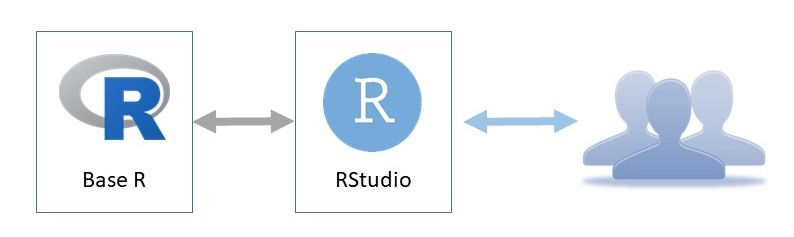
\includegraphics[width=0.6\linewidth]{img/baser_rstudio} 

}

\caption{How to use R – the best way}\label{fig:unnamed-chunk-2}
\end{figure}

Of course, we can use the \emph{Base R} directly. Usually, this is the only
option that is supported by mainframe environment. But, if you have the
opportunity, always use \emph{RStudio} instead of Basic R directly.

\begin{figure}

{\centering 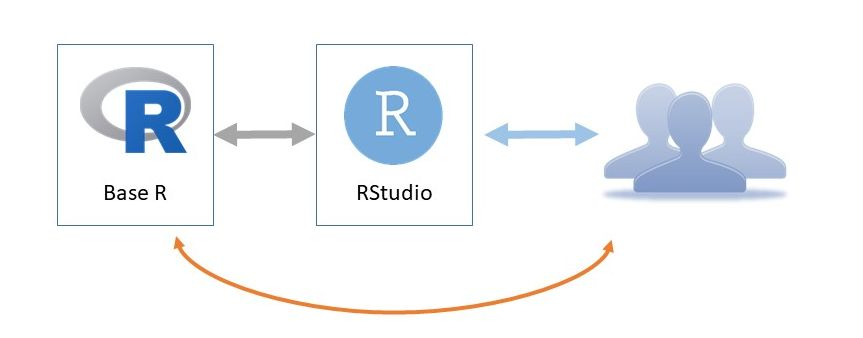
\includegraphics[width=0.6\linewidth]{img/baser_rstudio_min} 

}

\caption{How to use R – the minimum way}\label{fig:unnamed-chunk-3}
\end{figure}

Actually, there are several ways to use R, not only \emph{Base R} and
\emph{RStudio}. The table below summarizes the interfaces in the columns and
the tools in the rows. There are three different types of interface:
\emph{Console}, \emph{Script} and \emph{Point and clic}k. Interfaces allow the user to
interact with R.~

\begin{figure}

{\centering 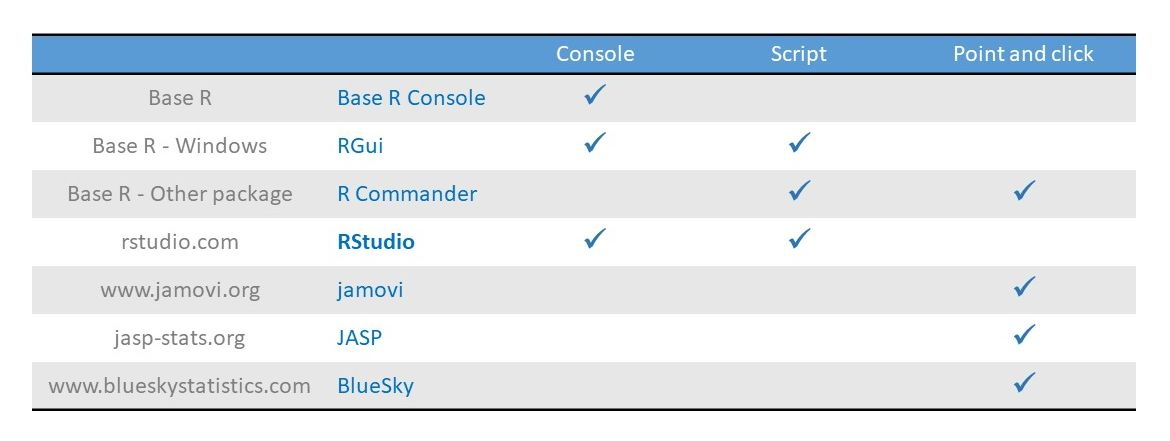
\includegraphics[width=0.9\linewidth]{img/baser_rstudio_all} 

}

\caption{How to use R – the minimum way}\label{fig:unnamed-chunk-4}
\end{figure}

\textbf{\emph{Console}} provides a command-line \emph{interface} that allows the user
to interact with the computer by typing commands . The computer displays
a prompt (\texttt{\textgreater{}}), the user types a command and presses Enter or
Return, and gets the result. There are three tools, that
provide console, the \emph{Base R} Console (it's the only option in mainframe
environment), \emph{RGui} in \emph{Base R} on Windows, and \emph{RStudio}.

The second interface is the \textbf{script interface}. It gives you an editor
window. You can type multiple lines of code into the source editor
without having each line evaluated by R. Then, when you're ready, you
can send the instructions to R - in other words, source the script -,
and you get the result. You can reach this functionality in \emph{RGui}, \emph{R
Commander} and \emph{RStudio}. \textbf{Remember, the best way to use R is creating,
editing and running scripts in \emph{RStudio}. This is the best option.}

For beginners, the best option would be to use a \textbf{Point-and-click
interface}. It has a menu, you can choose menupoints, menuitems, you
can get dialog boxes and type in editfields, point on radio buttons and
checkboxes. \textbf{But the knowledge of these systems have limits}. You can
execute only methods, which you can reach from the menu. The descriptive
measures, tables, plots and hypothesis tests, which you can point and
click, are part of knowledge of R. The whole knowledge can be reached
only from console or script interface. For example I only use \emph{jamovi},
if I have a simple question and I want to get a quick answer. ~So I
encourage you to install and try jamovi or JASP. These are free and user
friendly ways to do statistics. By the way, the tools I listed in this
table are all free, except the BlueSky. It is worth installing and
trying them.

\hypertarget{base-r}{%
\section{Base R}\label{base-r}}

What components were installed with \emph{Base R}? The \emph{Base R} consists of
three elements. The console for typing commands and getting results, the
interpreter for evaluating the commands, and packages for extending R's
knowledge. The interpreter is the heart of the R, all commands will be
executed by the interpreter. For the users, for us, the console is the
key. Apart from point and click interfaces, we will interact with the
console directly or indirectly.

\begin{figure}

{\centering 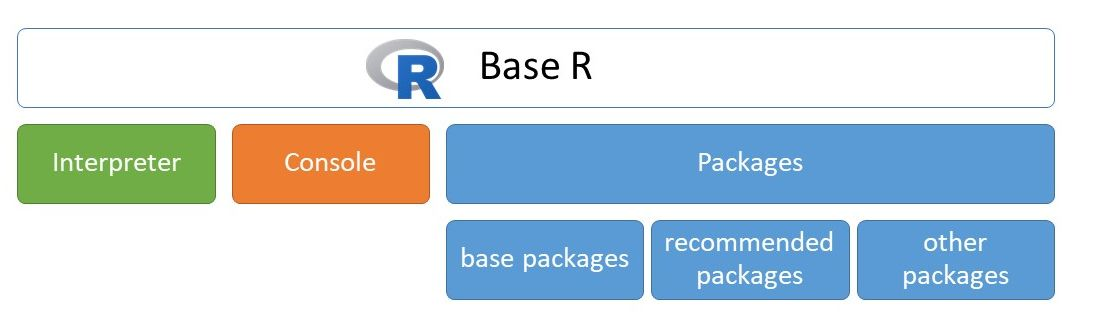
\includegraphics[width=0.7\linewidth]{img/baser} 

}

\caption{Components of Base R}\label{fig:unnamed-chunk-5}
\end{figure}

\hypertarget{console-of-base-r}{%
\subsection{Console of Base R}\label{console-of-base-r}}

As we mentioned, the R users meet the console all the time. One main
part of \emph{Base R} is the console. To start the console, we should type R
(the capital R letter) on all systems, or we can find and click on the R
icon. If you are on Windows, you can launch the \emph{R.exe} (e.g.
\texttt{c:\textbackslash{}Program\ Files\textbackslash{}R\textbackslash{}R-4.0.4\textbackslash{}bin\textbackslash{}x64\textbackslash{}R.exe}).

\begin{figure}

{\centering 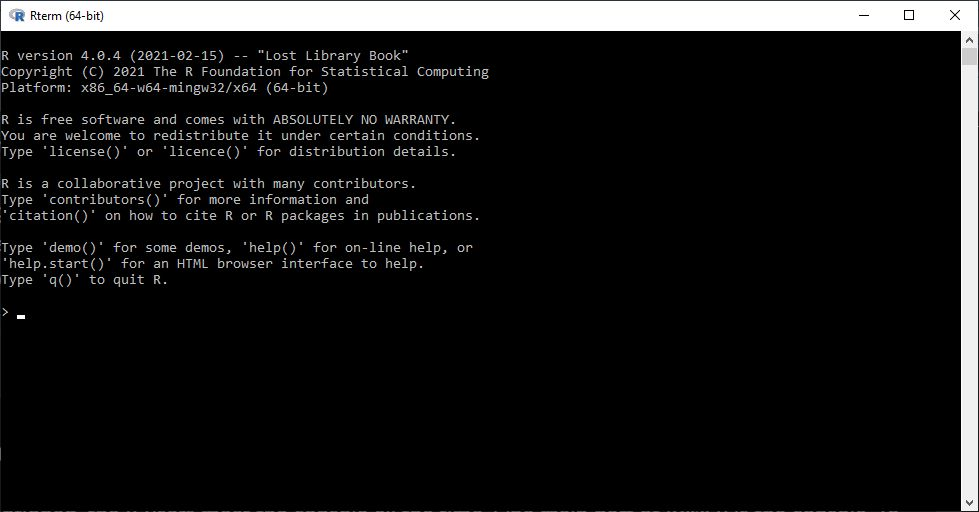
\includegraphics[width=0.7\linewidth]{img/console} 

}

\caption{Console in Base R}\label{fig:unnamed-chunk-6}
\end{figure}

On the screen above, you can see some information about the R instance.
At the bottom of the console window there is a prompt. It consists of a
`greater than' sign (symbol) and a space, and of course a cursor where
you can type any character.

Let's type any character, delete characters with Delete and
Backspace keys, move the cursor with Left arrow
and Right arrow keys, insert any character in this position,
and navigate the cursor the beginning of the line and the end of the
line with the Home and End keys.

If we are ready, we can execute this line, the command, hitting
Enter.

If the command is valid, R or more precisely its interpreter, will
execute it, then it returns the result in the console. If the command in
not valid, the interpreter returns an error message.

Let's start with numbers. Type 45 and hit Enter.

\begin{Shaded}
\begin{Highlighting}[]
\DecValTok{45}
\CommentTok{\#\textgreater{} [1] 45}
\end{Highlighting}
\end{Shaded}

This is a valid command because there is no error message. But the
result, the output, is meaningless.

Let's choose a more complicated expression:

\begin{Shaded}
\begin{Highlighting}[]
\DecValTok{45} \SpecialCharTok{+} \DecValTok{5}
\CommentTok{\#\textgreater{} [1] 50}
\end{Highlighting}
\end{Shaded}

Forty-five plus five sums fifty, so fifty is displayed in the output.
The 1 in brackets at the beginning of the output means this is the first
line of the output.

\hypertarget{console-features}{%
\subsubsection{Console features}\label{console-features}}

Every console has three features, that help us to execute commands.

\begin{description}
\item[History of commands]
We can use the Up arrow and Down arrow keys to
browse the history of commands, which we typed earlier. When you
press the Up arrow, you get the commands you typed
earlier at the command line. Of course you can modify them as well.
You can hit Enter at any time to run the command that is
currently displayed.
\item[Autocompletion]
Pressing TAB key completes the keyword or directory path
we were currently typing. Type in \texttt{getw} hit TAB and you
can see the whole function call, hitting Enter, you can
get the working directory.
\item[Continuation prompt]
Let's have a look at a small example. Tpye \texttt{45\ -}(forty-five minus)
and hit Enter. This is an invalid command, but we can not
see any Error message. Instead, a new prompt has appeared, a
continuation prompt indicated by a \texttt{+} (plus) followed by a space
character. We can continue typing. The console allows us to complete
the command. It's easy, type for example \texttt{5} (five), hit
Enter. We can get the result. I'll show you another
example. Type \texttt{getwd(} without closing parenthesis, hit
Enter. We will get the continuation prompt, and typing
closing parenthesis we get the working directory. It seems to help
us. Continuation prompt seems to be a good thing. But, It is not. It
is a really confusing feature. We can easily find ourselves in a
never ending story. We can type \texttt{45\ -}, Enter, \texttt{11\ *},
Enter and so on, we keep getting the continuation prompt,
and we don't really know how to complete it in a right way. So, It
is very important to leave the continuation prompt as soon as
possible. The key is Esc button. Lets' try this. Type in
opening parenthesis and 6 (\texttt{(6}), hit Enter, and press
Esc. We can get back the prompt `greater than' (\texttt{\textgreater{}}),
this is default prompt. When you see the plus prompt, continuation
prompt, you must press the Esc key.
\end{description}

\hypertarget{working-directory}{%
\subsubsection{Working directory}\label{working-directory}}

In R, we answer the questions we face using functions. So, the
expressions that we type into the command line, usually contains
\emph{function calls}. So, now, we can request the working directory. Let's
type \texttt{getwd()} to get the interpreter to display our working directory.

\begin{Shaded}
\begin{Highlighting}[]
\FunctionTok{getwd}\NormalTok{()}
\end{Highlighting}
\end{Shaded}

Working directory is the default directory that our command line reaches
to access files if we don't specify a path ourselves. We can specify
paths two ways either absolutely from the root directory or relatively
starting from our working directory. Beside reaching our history in the
command line we can also rely on the help of a built-in autocompletion
feature, by pressing TAB key, which completes the keyword or
directory path we were currently typing.

For example, let's type only \texttt{set} and press TAB and
TAB again to list out all the commands that start with \texttt{set}.
Press \texttt{w} and press TAB again, and as you can see the command
line completes our command with a \texttt{d} to get an existing function name.
All function call requires parentheses after the function name, which
contains additional data for the function which we call arguments.

The \texttt{setwd()} function has only one required arguments, which is a path
to a directory, which we want to set as our new working directory.

Let's try calling the \texttt{setwd()} function, start with the function name,
then the opening parenthesis and inside quote marks we give the
directory's path.

On Windows, after the first quote mark, type \texttt{c:/}, which refers the
drive you want to use, and press TAB twice to see all
subdirectories and files on the drive.

From here we can build our path directory by directory till we reach the
directory which we want to set as our working directory. As you can see
when jumping from directory into another we mark this jump with the
slash character. Instead of writing out the path ourselves we can write
the first few characters of directory's name and we can rely on
TAB to autocomplet it for us. Of course with more common
directory names we have to be more specific to get the desired
autocompletions.

Finally, if we reached our desired new working directory, we can execute
the command, by pressing enter, but make sure you have both your opening
and closing quote marks and parenthesis. If you had, your command
executed successfully thereby changing your working directory, but if
you made a mistake either in the formality of the command (called
syntactic error) or by giving a path to a directory which doesn't exist
(called semantic error).

To sum up, to set a working directory in R type:

\begin{Shaded}
\begin{Highlighting}[]
\FunctionTok{setwd}\NormalTok{(}\StringTok{"Path/To/Your/Workingdirectory"}\NormalTok{)}
\end{Highlighting}
\end{Shaded}

If you need to check which working directory R thinks it is in:

\begin{Shaded}
\begin{Highlighting}[]
\FunctionTok{getwd}\NormalTok{()}
\end{Highlighting}
\end{Shaded}

\hypertarget{quit-the-console}{%
\subsubsection{Quit the console}\label{quit-the-console}}

In the end, let's quit the console, by typing and executing the \texttt{q()}
command. Don't forget the parentheses. We don't need to save the
workspace. Choose \texttt{No}.

\hypertarget{rgui-on-windows}{%
\subsection{RGui on Windows}\label{rgui-on-windows}}

On Windows operating system, \emph{Base R} has another console which is more
advanced. The \emph{RGui} has a graphical user interface. To start it, find
and click on the R icon. You should always use the latest version and
the 64 bit version.

\begin{figure}

{\centering 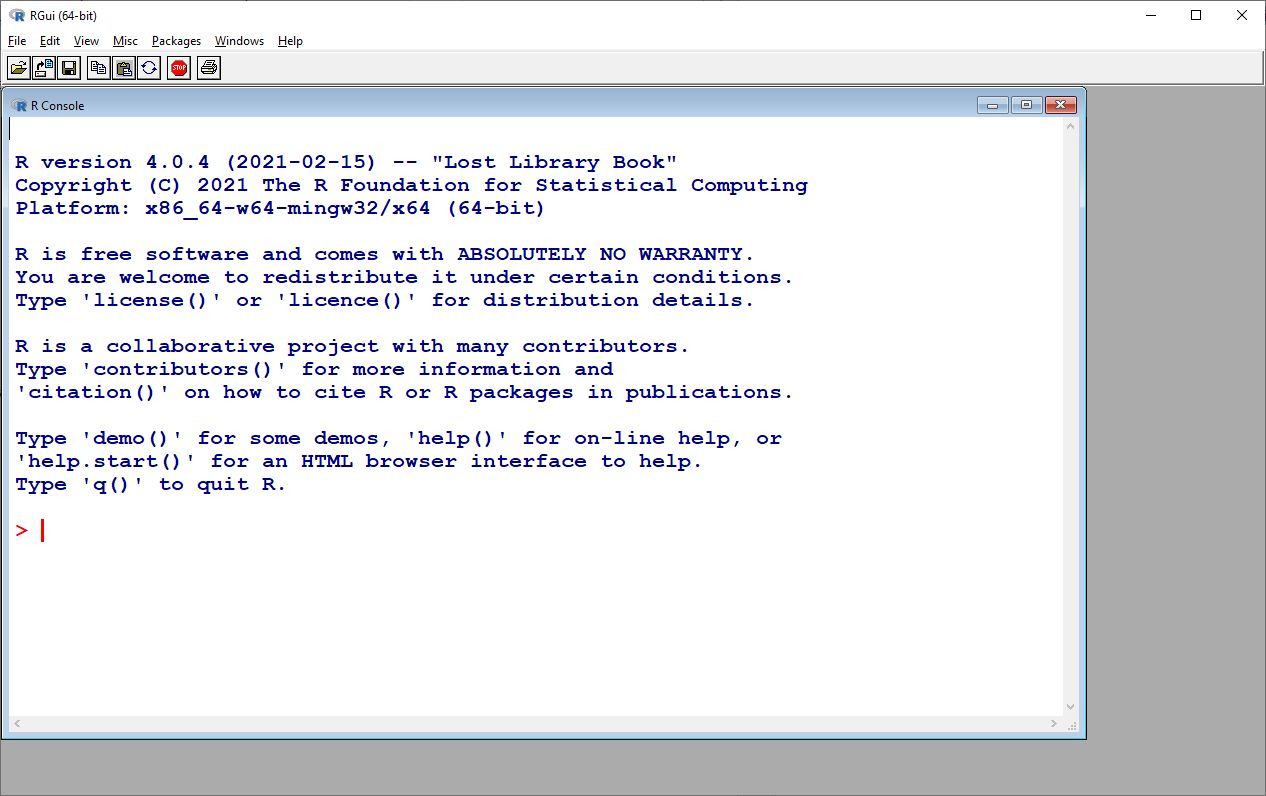
\includegraphics[width=0.7\linewidth]{img/rgui} 

}

\caption{Console in RGui}\label{fig:unnamed-chunk-12}
\end{figure}

Let's start up the aforementioned 64 bit version of it. Above you can
see our console which in functionality is the same as the one we used in
\emph{Base R} recently. We can type any character and press Enter.

If you'd like to change the appearance, or the size of the console, you
can do so in the \texttt{Edit\ \textgreater{}\ GUI\ preferences} menu in the upper menu bar.
Let's choose this menu item, and increase the font size to 28 and set
the style to bold. Close this dialog box with \texttt{OK} button, and you can
see a more readable console window. But as you can see we also have menu
and tool bar.

Let's try the same basic arithmetic command here. Type \texttt{45\ +\ 5} and
press Enter to execute it. And as we can see we get the same
result here.

Let's try the history with the Up arrow and Down
arrow. Navigate the cursor with Left arrow and
Right arrow keys, use the Home and End
buttons, insert or delete any character and press Enter.

\hypertarget{scripting-in-rgui}{%
\subsubsection{Scripting in RGui}\label{scripting-in-rgui}}

\emph{RGui} has all the functions the Console of \emph{Base R} had, and also a new
one. We can create script files with which we can use to store commands
in text files. Script files makes easy to store and organize commands.
So let's click \texttt{File\ \textgreater{}\ New\ script} which will make us a new script
window where you can edit your script file. We can arrange the Console
and Script windows, click on the \texttt{Windows\ \textgreater{}\ Tile\ horizontally}\textbf{.} You
can find the typical face of \emph{RGui} below.

\begin{figure}

{\centering 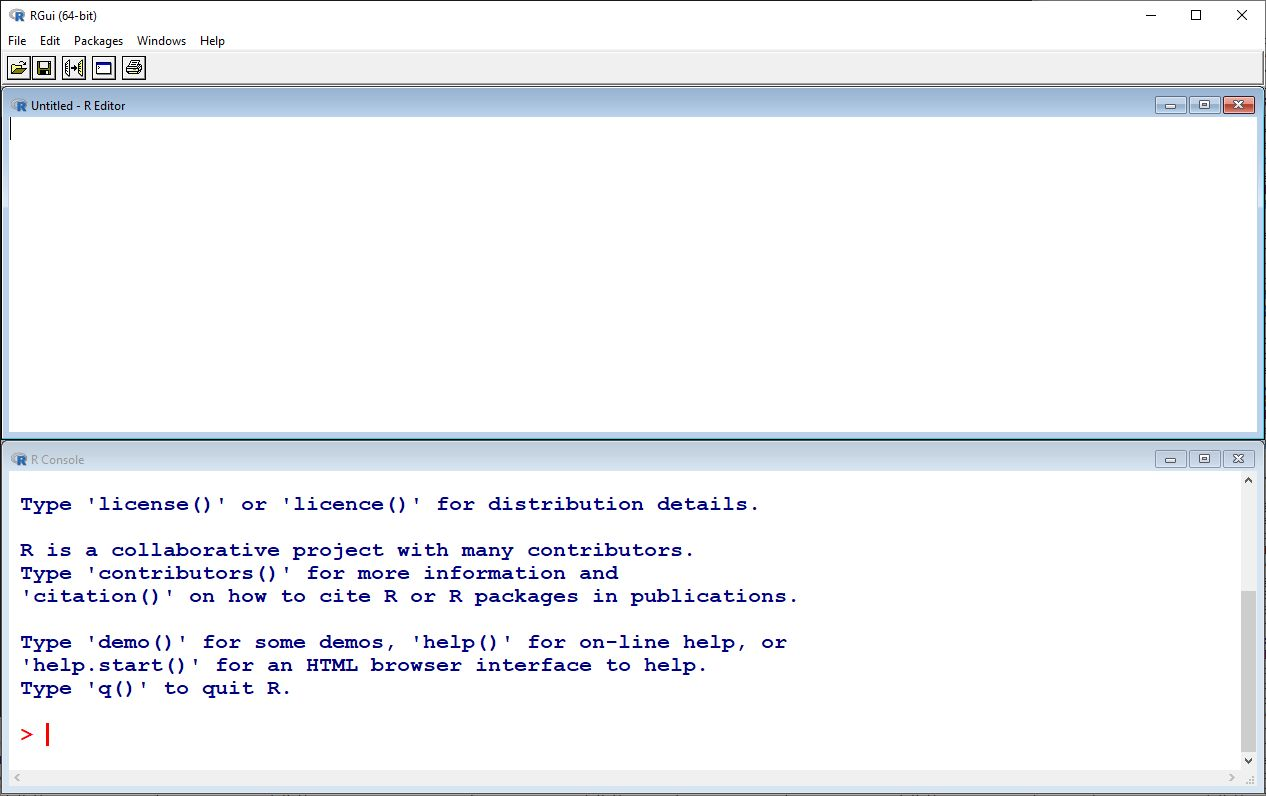
\includegraphics[width=0.7\linewidth]{img/rgui_script} 

}

\caption{Console in RGui}\label{fig:unnamed-chunk-13}
\end{figure}

Let's write the two commands in to this script file: \texttt{45\ +\ 5} and
\texttt{getwd()}.

Here we only type out command, to actually execute them we will need to
transfer them to the console. This window is only a text editor through
which we edit our script file. Here we can only use basic notepad like
functionalities, so no autocompletion or history.

We can move in a line with the Home and End
buttons and through lines with the Page Up and Page
Down buttons. With Ctrl+Home we can get to the
beginning of the script file and with Ctrl+End we can get to
the bottom of it. Of course, this comes handy with much larger script
files.

We can mark parts of the text with either holding the Shift
key and using the Left-Right-Up-Down arrow keys or using the
mouse. And we can use the clipboard as well, Ctrl+C,
Ctrl+X and Ctrl+V.

It's important to know how to actually execute the commands we just
wrote into our script file. With Ctrl+R we can execute the
line that our cursor is currently at. The process consists of the
command getting pulled into the console and then it executing it.

Let's try it. Move the cursor into the first line. Click in the first
line anywhere. Then press the Ctrl+R. Three things happened
at he same time. The first line was pulled into the console, the line
was executed, and the cursor jumped down a line. We can repress the
Ctrl+R and repeat the whole process for the second line. And
so on.

If you have any text selected in your editor prior, pressing
Ctrl+R, then the selected text will be executed. Let's also
try this. Select only \texttt{5\ +\ 5} from the first line, and press
Ctrl+R, and you get 10. Then, select the first two lines and
execute them with Ctrl+R. The interpreter ran both lines. You
can see the result in the console.

As you might have noticed, we have a colored console, the inputs, the
commands colored by red, and the outputs, the results colored by blue.

This script files can also contain comments, which is useful to mark
what's the command's intention. Which ones again may seem unimportant
now, but is really useful when working with massive script files.

To mark something as a comment use the hash mark (\texttt{\#}) which marks
everything in a line after the hash mark as a comment. It's good
practice to start your script file with 3 comment lines which contains
the author of the file, the date and a name which gives some kind of
information about what the script does.

\begin{Shaded}
\begin{Highlighting}[]
\CommentTok{\# Kálmán Abari}
\CommentTok{\# 2021{-}03{-}17}
\CommentTok{\# First script file}
\end{Highlighting}
\end{Shaded}

Navigate the cursor to the first position of the file, for example
pressing the Ctrl+Home. Then type a hash mark, and your name,
Enter. Hash mark, date of today, Enter, hash mark
\texttt{First\ script\ file}, Enter.

If we are ready, we are going to save the script file. It's important to
save the script file with the \texttt{File\ \textgreater{}\ Save} menu. It's good practice to
save your work every 15 minutes. It's important that when we save our
files we give them names that doesn't contain any special characters or
whitespaces, underscores are acceptable though. Choose a proper
directory and type in \texttt{first\_script.R} as the filename. Make sure that
our file's extension should be \texttt{.R} which means that it contains an R
script file.

With that we covered the basics of the \emph{RGui}, so we can close it for
now, we shouldn't worry about saving our workspace since we won't be
needing it.

\hypertarget{rstudio}{%
\section{RStudio}\label{rstudio}}

The last tool we will get to know now and will be using for the rest of
the book is \emph{RStudio}. We can also launch it from the start menu. While
we had multiple \emph{Basic R} instances, we only have one \emph{RStudio}, so it
should be easy to find it.

It's the most advanced interface to use R from the aforementioned ones.
And this will be the one that we will mainly use through out the course.
Even though we will only use \emph{RStudio}, it's important to mention that
RStudio relies on \emph{Base R} to work.

\hypertarget{customization}{%
\subsection{Customization}\label{customization}}

We can easily check which instance of \emph{Base R} our \emph{RStudio} is using.
We can see this in the \texttt{Global\ options\ \textgreater{}\ Tools} menu option.

Let's check if it really is using the 64 bit version.

Here we can also do other customizations. While we're here we should
also uncheck the \texttt{Restore\ .Rdata} option and set the
\texttt{Save\ workspace\ to\ Rdata\ on\ exit} option to \texttt{Never}.

Another important one is the \texttt{Code} menu point from the left list. Here
under the \texttt{Saving} option we have to set the \texttt{Default\ text\ encoding} to
\texttt{UTF-8} which is a wildly used and accepted character-code standard.

You can customize to look of your editor under the \texttt{Appearance} option.
Here you can change the theme of your editor, which is sets the color
palette it uses. I recommend changing it to \texttt{Tomorrow\ night\ bright}.
Let's close the settings, by pressing \texttt{OK}, to save the changes we made.

\hypertarget{using-rstudio}{%
\subsection{Using RStudio}\label{using-rstudio}}

A few words about RStudio. The main area consists of 3 or 4 different
panes or windows which all are responsible for a different task. You
have 3 panes by basic. The fourth panes you can add is a script file
editor, which you can do by creating a new script file in
\texttt{File\ \textgreater{}\ New\ file\ \textgreater{}-\/-\ R\ Script}.

\begin{figure}
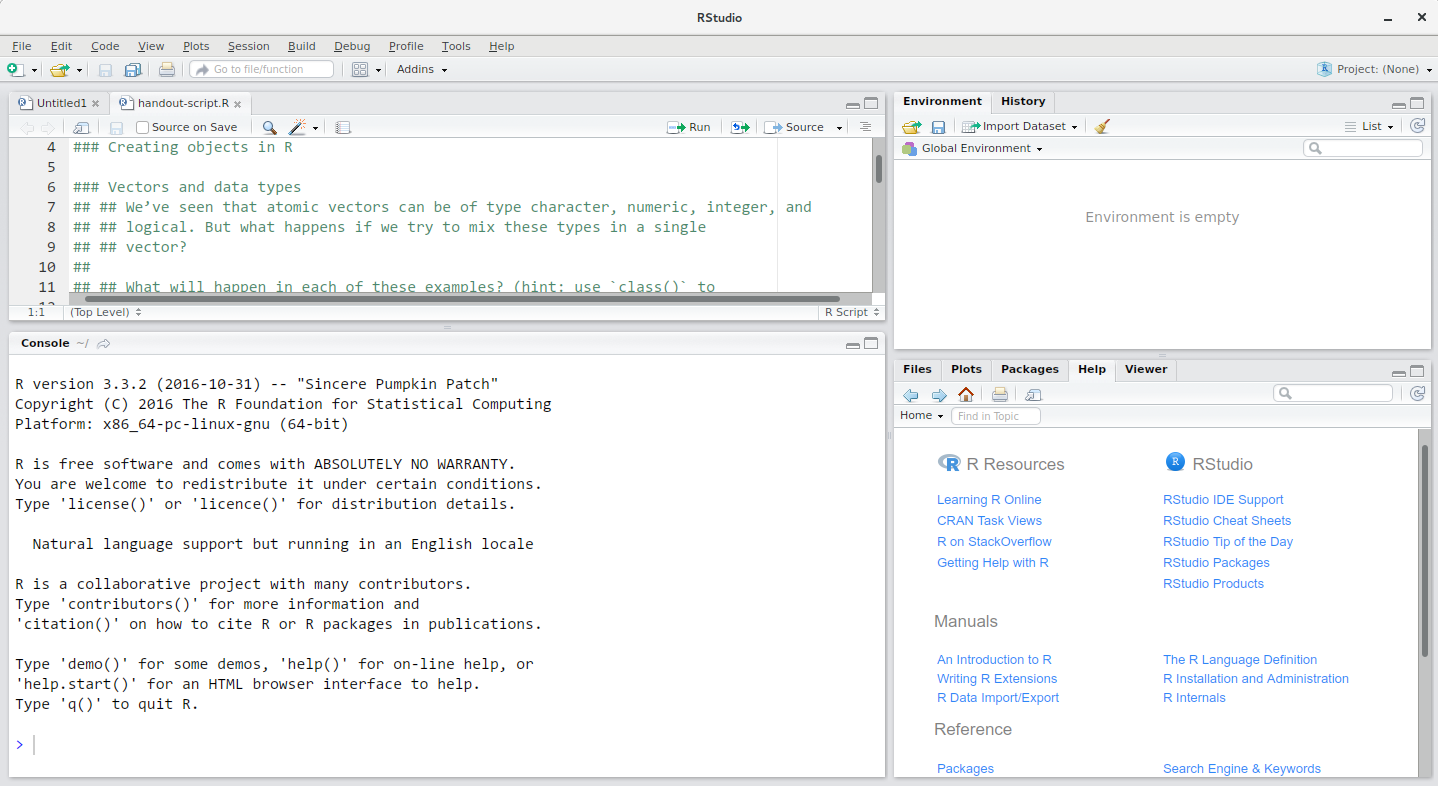
\includegraphics[width=1\linewidth]{img/rstudio-screenshot} \caption{The RStudio Interface}\label{fig:RStudio-GUI}
\end{figure}

You can easily resize the panes with clicking and dragging the vertical
or horizontal line between the panes.

RStudio is divided into 4 ``Panes'':

\begin{itemize}
\tightlist
\item
  the \textbf{Source} for your scripts and documents (top-left, in the
  default layout),
\item
  the R \textbf{Console} (bottom-left),
\item
  your \textbf{Environment/History} (top-right), and
\item
  your \textbf{Files/Plots/Packages/Help/Viewer} (bottom-right).
\end{itemize}

The placement of these panes and their content can be customized (see
main Menu \texttt{Tools\ \textgreater{}\ Global\ Options\ \textgreater{}\ Pane\ Layout}. One of the advantages
of using \texttt{RStudio} is that all the information you need to write code is
available in a single window.

\hypertarget{how-to-start-an-r-project}{%
\subsection{How to start an R project}\label{how-to-start-an-r-project}}

It is good practice to keep a set of related data, analyses, and text
self-contained in a single folder. When working with R and RStudio you
typically want that single top folder to be the folder you are working
in. In order to tell R this, you will want to set that folder as your
\textbf{working directory}. Whenever you refer to other scripts or data or
directories contained within the working directory you can then use
\emph{relative paths} to files that indicate where inside the project a file
is located. (That is opposed to absolute paths, which point to where a
file is on a specific computer). Having everything contained in a single
directory makes it a lot easier to move your project around on your
computer and share it with others without worrying about whether or not
the underlying scripts will still work.

Whenever you create a project with \emph{RStudio} it creates a working
directory for you and remembers its location (allowing you to quickly
navigate to it) and optionally preserves custom settings and open files
to make it easier to resume work after a break. Below, we will go
through the steps for creating an ``R Project'' for this workshop.

\begin{itemize}
\tightlist
\item
  Start RStudio
\item
  Under the \texttt{File} menu, click on \texttt{New\ project}, choose
  \texttt{New\ directory}, then \texttt{Empty\ project}
\item
  As directory (or folder) name enter \texttt{r-intro} and create project as
  subdirectory of your desktop folder: \texttt{\textasciitilde{}/Desktop}
\item
  Click on \texttt{Create\ project}
\item
  Under the \texttt{Files} tab on the right of the screen, click on
  \texttt{New\ Folder} and create a folder named \texttt{data} within your newly
  created working directory (e.g., \texttt{\textasciitilde{}/r-intro/data})
\item
  On the main menu go to \texttt{Files} \textgreater{} \texttt{New\ File} \textgreater{} \texttt{R\ Script} (or use
  the shortcut Ctrl+Shift+\texttt{N}) to open a new file
\item
  Save the empty script as \texttt{r-intro-script.R} in your working
  directory.
\end{itemize}

Your working directory should now look like in Figure
\ref{fig:working-dir}.

\begin{figure}
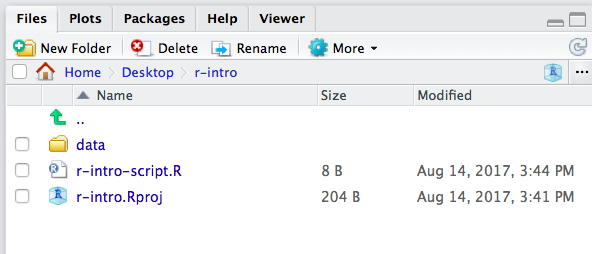
\includegraphics[width=0.6\linewidth]{img/Rproject-setup} \caption{What it should look like at the beginning of this lesson}\label{fig:working-dir}
\end{figure}

\hypertarget{organizing-your-working-directory}{%
\subsection{Organizing your working directory}\label{organizing-your-working-directory}}

Using a consistent folder structure across your projects will help keep
things organized, and will also make it easy to find/file things in the
future. This can be especially helpful when you have multiple projects.
In general, you may create directories (folders) for \textbf{data},
\textbf{documents}, and \textbf{outputs}.

\begin{itemize}
\tightlist
\item
  \textbf{\texttt{data/}} Use this folder to store your raw input data.
\item
  \textbf{\texttt{documents/}} If you are working on a paper this would be a place
  to keep outlines, drafts, and other text.
\item
  \textbf{\texttt{output/}} Use this folder to store your intermediate or final
  datasets and images you may create for the need of a particular
  analysis. For the sake of transparency, you should \emph{always} keep a
  copy of your raw data accessible and do as much of your data cleanup
  and preprocessing programmatically, You could have subfolders in
  your \texttt{output} directory named \texttt{output/data} that would contain the
  respective processed files. I also like to save my images in
  \texttt{output/image} directory.
\end{itemize}

You may want additional directories or subdirectories depending on your
project needs, but this is a good template to form the backbone of your
working directory.

\hypertarget{rstudio-console-and-command-prompt}{%
\subsection{RStudio Console and Command Prompt}\label{rstudio-console-and-command-prompt}}

The console pane in RStudio is the place where commands written in the R
language can be typed and executed immediately by the computer. It is
also where the results will be shown for commands that have been
executed. You can type commands directly into the console and press
Enter to execute those commands, but they will be forgotten
when you close the session.

If R is ready to accept commands, the R console by default shows a \texttt{\textgreater{}}
prompt. If it receives a command (by typing, copy-pasting or sent from
the script editor using Ctrl Enter), R will try to execute
it, and when ready, will show the results and come back with a new \texttt{\textgreater{}}
prompt to wait for new commands.

If R is still waiting for you to enter more data because it isn't
complete yet, the console will show a \texttt{+} prompt. It means that you
haven't finished entering a complete command. This is because you have
not `closed' a parenthesis or quotation, i.e.~you don't have the same
number of left-parentheses as right-parentheses, or the same number of
opening and closing quotation marks. When this happens, and you thought
you finished typing your command, click inside the console window and
press Esc; this will cancel the incomplete command and return
you to the \texttt{\textgreater{}} prompt.

\hypertarget{rstudio-script-editor}{%
\subsection{RStudio Script Editor}\label{rstudio-script-editor}}

Because we want to keep our code and workflow, it is better to type the
commands we want in the script editor, and save the script. This way,
there is a complete record of what we did, and anyone (including our
future selves!) can easily replicate the results on their computer.

Perhaps one of the most important aspects of making your code
comprehensible for others and your future self is adding comments about
why you did something. You can write comments directly in your script,
and tell R not no execute those words simply by putting a hashtag (\texttt{\#})
before you start typing the comment.

\begin{Shaded}
\begin{Highlighting}[]
\CommentTok{\# this is a comment on its on line}
\FunctionTok{getwd}\NormalTok{() }\CommentTok{\# comments can also go here}
\end{Highlighting}
\end{Shaded}

One of the first things you will notice is in the R script editor that
your code is colored (syntax coloring) which enhances readability.

Secondly, RStudio allows you to execute commands directly from the
script editor by using the Ctrl + Enter shortcut (on Macs,
Cmd + Enter will work, too). The command on the current line
in the script (indicated by the cursor) or all of the commands in the
currently selected text will be sent to the console and executed when
you press Ctrl + Enter. You can find other keyboard shortcuts
under \texttt{Tools} \textgreater{} \texttt{Keyboard\ Shortcuts\ Help} (or \texttt{Alt} +
\texttt{Shift} + \texttt{K})

At some point in your analysis you may want to check the content of a
variable or the structure of an object, without necessarily keeping a
record of it in your script. You can type these commands and execute
them directly in the console. RStudio provides the Ctrl + 1
and \texttt{Ctrl} + \texttt{2} shortcuts allow you to jump
between the script and the console panes.

All in all, RStudio is designed to make your coding easier and less
error-prone.

\hypertarget{rmarkdown}{%
\section{RMarkdown}\label{rmarkdown}}

\hypertarget{introduction}{%
\subsection{Introduction}\label{introduction}}

RMarkdown allows you write reports that include both R codes and the
output generated. Moreover, these reports are dynamic in the sense that
changing the data and reprocessing the file will result in a new report
with updated output. RMarkdown also lets you include Latex math,
hyperlinks and images. These dynamic reports can be saved as

\begin{itemize}
\tightlist
\item
  PDF or PostScript documents
\item
  Web pages
\item
  Microsoft Word documents
\item
  Open Document files
\item
  and more like Beamer slides, etc.
\end{itemize}

When you render an RMarkdown file, it will appear, by default, as an
HTML document in Viewer window of RStudio. If you want to create PDF
documents, install a LaTeX compiler. Install MacTeX for Macs (\url{http://}
tug.org/mactex), MiKTeX (www.miktex.org) for Windows, and TeX Live for
Linux (www.tug.org/texlive). Alternatively, you can install TinyTeX from
\url{https://yihui.name/tinytex/}.

\hypertarget{basic-structure-of-r-markdown}{%
\subsection{Basic Structure of R Markdown}\label{basic-structure-of-r-markdown}}

Let's start with a simple RMarkdown file and see what it looks like and
the output that it produces when executed. Click
\texttt{File\ \textgreater{}\ New\ File\ \textgreater{}\ R\ Markdown}, type in the title \texttt{Homework\ problems},
and the author. Click \texttt{OK}. Save the file with Ctrl+S, choose
a name for example, \texttt{homework\_1.Rmd}.

Rmarkdown files ends with the \texttt{.Rmd} extension. An \texttt{.Rmd} file contains
three types of contents:

\begin{enumerate}
\def\labelenumi{\arabic{enumi}.}
\tightlist
\item
  A YAML header :
\end{enumerate}

\begin{Shaded}
\begin{Highlighting}[]
\PreprocessorTok{{-}{-}{-}}
\FunctionTok{title}\KeywordTok{:}\AttributeTok{ }\StringTok{"Homework problems"}
\FunctionTok{author}\KeywordTok{:}\AttributeTok{ }\StringTok{"Abari Kálmán"}
\FunctionTok{date}\KeywordTok{:}\AttributeTok{ }\StringTok{\textquotesingle{}2021 03 31 \textquotesingle{}}
\FunctionTok{output}\KeywordTok{:}\AttributeTok{ html\_document}
\PreprocessorTok{{-}{-}{-}}
\end{Highlighting}
\end{Shaded}

YAML stands for ``yet another markup language''
(\url{https://en.wikipedia.org/wiki/YAML}).

\begin{enumerate}
\def\labelenumi{\arabic{enumi}.}
\setcounter{enumi}{1}
\tightlist
\item
  R code chuncks. For example:
\end{enumerate}

\begin{Shaded}
\begin{Highlighting}[]
\InformationTok{\textasciigrave{}\textasciigrave{}\textasciigrave{}\{r\}}
\InformationTok{myDataFrame \textless{}{-} data.frame(names = LETTERS[1:3], variable\_1 = runif(3))}
\InformationTok{myDataFrame}
\InformationTok{\textasciigrave{}\textasciigrave{}\textasciigrave{}}
\end{Highlighting}
\end{Shaded}

\begin{enumerate}
\def\labelenumi{\arabic{enumi}.}
\setcounter{enumi}{2}
\tightlist
\item
  Text with formatting like bold text, mathematical expressions (), or
  headings \# Heading, etc.
\end{enumerate}

First let's see how we can execute an \texttt{.Rmd} file to produce the output
as PDF, HTML, etc.

Now click \texttt{Knit} to produce a complete report containing all text, code,
and results. Alternatively, pressing Ctrl+Shift+K renders the
whole document. But in this case, all output formats that are specified
in the YAML header will be produced. On the other hand, Knit allows you
to specify the output format you want to produce. For example,
\texttt{Knit\ \textgreater{}\ Knit\ to\ HTML} produces only HTML output, which is usually faster
than producing PDF output.

You can also render the file programmatically with the following
command:

\begin{Shaded}
\begin{Highlighting}[]
\NormalTok{rmarkdown}\SpecialCharTok{::}\FunctionTok{render}\NormalTok{(}\StringTok{"homework\_1.Rmd"}\NormalTok{) }
\end{Highlighting}
\end{Shaded}

This will display the report in the viewer pane, and create a
self-contained HTML file.

Instead of running the whole document, you can run each individual code
chunk by clicking the Run icon at the top right of the chunk or by
pressing Ctrl+Shift+Enter. RStudio executes the code and
displays the results inline with the code.

\hypertarget{text-formatting-with-r-markdown}{%
\subsection{Text Formatting with R Markdown}\label{text-formatting-with-r-markdown}}

This section demonstrates the syntax of common components of a document
written in R Markdown. Inline text will be \emph{italic} if surrounded by
underscores or asterisks, e.g., \texttt{\_text\_} or \texttt{*text*}. \textbf{Bold} text is
produced using a pair of double asterisks (\texttt{**text**}). A pair of tildes
(\texttt{\textasciitilde{}}) turn text to a subscript (e.g., \texttt{H\textasciitilde{}3\textasciitilde{}PO\textasciitilde{}4\textasciitilde{}} renders H\textsubscript{3}PO\textsubscript{4}). A
pair of carets (\texttt{\^{}}) produce a superscript (e.g., \texttt{Cu\^{}2+\^{}} renders
Cu\textsuperscript{2+}).

Hyperlinks are created using the syntax \texttt{{[}text{]}(link)}, e.g.,
\texttt{{[}RStudio{]}(https://www.rstudio.com)}. The syntax for images is similar:
just add an exclamation mark, e.g.,
\texttt{!{[}alt\ text\ or\ image\ title{]}(path/to/image)}. Footnotes are put inside
the square brackets after a caret \texttt{\^{}{[}{]}}, e.g., \texttt{\^{}{[}This\ is\ a\ footnote.{]}}.

Section headers can be written after a number of pound signs, e.g.,

\begin{Shaded}
\begin{Highlighting}[]
\FunctionTok{\# First{-}level header}

\FunctionTok{\#\# Second{-}level header}

\FunctionTok{\#\#\# Third{-}level header}
\end{Highlighting}
\end{Shaded}

If you do not want a certain heading to be numbered, you can add \texttt{\{-\}}
or \texttt{\{.unnumbered\}} after the heading, e.g.,

\begin{Shaded}
\begin{Highlighting}[]
\FunctionTok{\# Preface \{{-}\}}
\end{Highlighting}
\end{Shaded}

Unordered list items start with \texttt{*}, \texttt{-}, or \texttt{+}, and you can nest one
list within another list by indenting the sub-list, e.g.,

\begin{Shaded}
\begin{Highlighting}[]
\SpecialStringTok{{-} }\NormalTok{one item}
\SpecialStringTok{{-} }\NormalTok{one item}
\SpecialStringTok{{-} }\NormalTok{one item}
\SpecialStringTok{    {-} }\NormalTok{one more item}
\SpecialStringTok{    {-} }\NormalTok{one more item}
\SpecialStringTok{    {-} }\NormalTok{one more item}
\end{Highlighting}
\end{Shaded}

The output is:

\begin{itemize}
\item
  one item
\item
  one item
\item
  one item

  \begin{itemize}
  \tightlist
  \item
    one more item
  \item
    one more item
  \item
    one more item
  \end{itemize}
\end{itemize}

Ordered list items start with numbers (you can also nest lists within
lists), e.g.,

\begin{Shaded}
\begin{Highlighting}[]
\SpecialStringTok{1. }\NormalTok{the first item}
\SpecialStringTok{2. }\NormalTok{the second item}
\SpecialStringTok{3. }\NormalTok{the third item}
\SpecialStringTok{    {-} }\NormalTok{one unordered item}
\SpecialStringTok{    {-} }\NormalTok{one unordered item}
\end{Highlighting}
\end{Shaded}

The output does not look too much different with the Markdown source:

\begin{enumerate}
\def\labelenumi{\arabic{enumi}.}
\item
  the first item
\item
  the second item
\item
  the third item

  \begin{itemize}
  \tightlist
  \item
    one unordered item
  \item
    one unordered item
  \end{itemize}
\end{enumerate}

Blockquotes are written after \texttt{\textgreater{}}, e.g.,

\begin{Shaded}
\begin{Highlighting}[]
\AttributeTok{\textgreater{} "I thoroughly disapprove of duels. If a man should challenge me,}
\AttributeTok{  I would take him kindly and forgivingly by the hand and lead him}
\AttributeTok{  to a quiet place and kill him."}
\AttributeTok{\textgreater{}}
\AttributeTok{\textgreater{} {-}{-}{-} Mark Twain}
\end{Highlighting}
\end{Shaded}

The actual output (we customized the style for blockquotes in this
book):

\begin{quote}
``I thoroughly disapprove of duels. If a man should challenge me, I
would take him kindly and forgivingly by the hand and lead him to a
quiet place and kill him.''

--- Mark Twain
\end{quote}

Plain code blocks can be written after three or more backticks, and you
can also indent the blocks by four spaces, e.g.,

\begin{Shaded}
\begin{Highlighting}[]
\InformationTok{\textasciigrave{}\textasciigrave{}\textasciigrave{}}
\InformationTok{This text is displayed verbatim / preformatted}
\InformationTok{\textasciigrave{}\textasciigrave{}\textasciigrave{}}

\NormalTok{Or indent by four spaces:}

\InformationTok{    This text is displayed verbatim / preformatted}
\end{Highlighting}
\end{Shaded}

In general, you'd better leave at least one empty line between adjacent
but different elements, e.g., a header and a paragraph. This is to avoid
ambiguity to the Markdown renderer. For example, does ``\texttt{\#}'' indicate a
header below?

\begin{Shaded}
\begin{Highlighting}[]
\NormalTok{In R, the character}
\FunctionTok{\# indicates a comment.}
\end{Highlighting}
\end{Shaded}

And does ``\texttt{-}'' mean a bullet point below?

\begin{Shaded}
\begin{Highlighting}[]
\NormalTok{The result of 5}
\SpecialStringTok{{-} }\NormalTok{3 is 2.}
\end{Highlighting}
\end{Shaded}

Different flavors of Markdown may produce different results if there are
no blank lines.

\hypertarget{math-expressions}{%
\subsection{Math expressions}\label{math-expressions}}

Inline LaTeX equations\index{LaTeX math} can be written in a pair of
dollar signs using the LaTeX syntax, e.g.,
\texttt{\$f(k)\ =\ \{n\ \textbackslash{}choose\ k\}\ p\^{}\{k\}\ (1-p)\^{}\{n-k\}\$} (actual output:
\(f(k)={n \choose k}p^{k}(1-p)^{n-k}\)); math expressions of the display
style can be written in a pair of double dollar signs, e.g.,
\texttt{\$\$f(k)\ =\ \{n\ \textbackslash{}choose\ k\}\ p\^{}\{k\}\ (1-p)\^{}\{n-k\}\$\$}, and the output looks like
this:

\[f\left(k\right)=\binom{n}{k}p^k\left(1-p\right)^{n-k}\]

You can also use math environments inside \texttt{\$\ \$} or \texttt{\$\$\ \$\$}, e.g.,

\begin{Shaded}
\begin{Highlighting}[]
\SpecialStringTok{$$}\KeywordTok{\textbackslash{}begin}\NormalTok{\{}\ExtensionTok{array}\NormalTok{\}}\SpecialStringTok{\{ccc\}}
\SpecialStringTok{x\_\{11\} \& x\_\{12\} \& x\_\{13\}}\SpecialCharTok{\textbackslash{}\textbackslash{}}
\SpecialStringTok{x\_\{21\} \& x\_\{22\} \& x\_\{23\}}
\KeywordTok{\textbackslash{}end}\NormalTok{\{}\ExtensionTok{array}\NormalTok{\}}\SpecialStringTok{$$}
\end{Highlighting}
\end{Shaded}

\[\begin{array}{ccc}
x_{11} & x_{12} & x_{13}\\
x_{21} & x_{22} & x_{23}
\end{array}\]

\begin{Shaded}
\begin{Highlighting}[]
\SpecialStringTok{$$X = }\KeywordTok{\textbackslash{}begin}\NormalTok{\{}\ExtensionTok{bmatrix}\NormalTok{\}}\SpecialStringTok{1 \& x\_\{1\}}\SpecialCharTok{\textbackslash{}\textbackslash{}}
\SpecialStringTok{1 \& x\_\{2\}}\SpecialCharTok{\textbackslash{}\textbackslash{}}
\SpecialStringTok{1 \& x\_\{3\}}
\KeywordTok{\textbackslash{}end}\NormalTok{\{}\ExtensionTok{bmatrix}\NormalTok{\}}\SpecialStringTok{$$}
\end{Highlighting}
\end{Shaded}

\[X = \begin{bmatrix}1 & x_{1}\\
1 & x_{2}\\
1 & x_{3}
\end{bmatrix}\]

\begin{Shaded}
\begin{Highlighting}[]
\SpecialStringTok{$$}\SpecialCharTok{\textbackslash{}Theta}\SpecialStringTok{ = }\KeywordTok{\textbackslash{}begin}\NormalTok{\{}\ExtensionTok{pmatrix}\NormalTok{\}}\SpecialCharTok{\textbackslash{}alpha}\SpecialStringTok{ \& }\SpecialCharTok{\textbackslash{}beta\textbackslash{}\textbackslash{}}
\SpecialCharTok{\textbackslash{}gamma}\SpecialStringTok{ \& }\SpecialCharTok{\textbackslash{}delta}
\KeywordTok{\textbackslash{}end}\NormalTok{\{}\ExtensionTok{pmatrix}\NormalTok{\}}\SpecialStringTok{$$}
\end{Highlighting}
\end{Shaded}

\[\Theta = \begin{pmatrix}\alpha & \beta\\
\gamma & \delta
\end{pmatrix}\]

\begin{Shaded}
\begin{Highlighting}[]
\SpecialStringTok{$$}\KeywordTok{\textbackslash{}begin}\NormalTok{\{}\ExtensionTok{vmatrix}\NormalTok{\}}\SpecialStringTok{a \& b}\SpecialCharTok{\textbackslash{}\textbackslash{}}
\SpecialStringTok{c \& d}
\KeywordTok{\textbackslash{}end}\NormalTok{\{}\ExtensionTok{vmatrix}\NormalTok{\}}\SpecialStringTok{=ad{-}bc$$}
\end{Highlighting}
\end{Shaded}

\[\begin{vmatrix}a & b\\
c & d
\end{vmatrix}=ad-bc\]

\hypertarget{the-r-language}{%
\chapter{The R language}\label{the-r-language}}

\hypertarget{basic-data-type}{%
\section{Basic data type}\label{basic-data-type}}

It this chapter, we'll focus on R language. First, we need to learn about data types. The R programming language has something called types, and there are four of them:

\begin{itemize}
\tightlist
\item
  character
\item
  integer
\item
  double
\item
  logical.
\end{itemize}

Let's take a look at each one of these. Let's start with double.

\hypertarget{double}{%
\subsection{Double}\label{double}}

We can easily create numbers in R. For example:

\begin{Shaded}
\begin{Highlighting}[]
\DecValTok{45}
\CommentTok{\#\textgreater{} [1] 45}
\DecValTok{5}
\CommentTok{\#\textgreater{} [1] 5}
\FloatTok{0.5}
\CommentTok{\#\textgreater{} [1] 0.5}
\SpecialCharTok{{-}}\FloatTok{0.33}
\CommentTok{\#\textgreater{} [1] {-}0.33}
\end{Highlighting}
\end{Shaded}

We can execute these lines, these are simple commands, more precisely numerical \emph{constants}. These elements of R language have a fix value. We can't change the value of a constant. The \texttt{0.5} means 0.5. So executing of \texttt{0.5} five we get 0.5 in R console. Decimals omitting the leading zero are acceptable, we can write \texttt{.5}. It means 0.5. So, we can get a tricky form of a number for example \texttt{-.5}, which means -0.5. You can check this out executing these lines.

\begin{Shaded}
\begin{Highlighting}[]
\SpecialCharTok{{-}}\NormalTok{.}\DecValTok{5}
\CommentTok{\#\textgreater{} [1] {-}0.5}
\end{Highlighting}
\end{Shaded}

We are going to move on to discuss the exponential format of numbers. This is the scientific notation, where the number after `e' gives the powers of ten. For example \texttt{4e2} means 400, because 4 multiplied by 10 squared is 400 (4 multiplied by 10 the power of 2).

\begin{Shaded}
\begin{Highlighting}[]
\FloatTok{4e2}
\CommentTok{\#\textgreater{} [1] 400}
\end{Highlighting}
\end{Shaded}

Generally, we use plus-minus sign before the power, for example \texttt{4e+3}, which value is 4000, \texttt{4.2e+3} means 4200, and \texttt{4.2e-3} means 0.0042. In this case, we have to divide by 10 cubed (10 to the power of 3), or multiplied by ten to the power of -3.

\begin{Shaded}
\begin{Highlighting}[]
\FloatTok{4e+3}
\CommentTok{\#\textgreater{} [1] 4000}
\FloatTok{4.2e+3}
\CommentTok{\#\textgreater{} [1] 4200}
\FloatTok{4.2e{-}3}
\CommentTok{\#\textgreater{} [1] 0.0042}
\end{Highlighting}
\end{Shaded}

The last format of numbers is the hexadecimal. For example after '0x' prefix, we can type \texttt{0xfe3} which means 4067.

\begin{Shaded}
\begin{Highlighting}[]
\DecValTok{0xfe3}
\CommentTok{\#\textgreater{} [1] 4067}
\end{Highlighting}
\end{Shaded}

The hexadecimal numbering system uses 16 as the base (as opposed to ten), so in this system we have 16 digits to represent numbers. The symbols ``0''--``9'' to represent values 0 to 9, and ``A''-``F'' (or alternatively ``a''-``f'') to represent values 10 to 15.

We use hexadecimal at most, when we specify a color. For example:

\begin{Shaded}
\begin{Highlighting}[]
\FunctionTok{plot}\NormalTok{(}\DecValTok{1}\NormalTok{, }\AttributeTok{col=}\StringTok{"\#ee0000"}\NormalTok{, }\AttributeTok{pch=}\DecValTok{16}\NormalTok{, }\AttributeTok{cex=}\DecValTok{8}\NormalTok{)}
\end{Highlighting}
\end{Shaded}

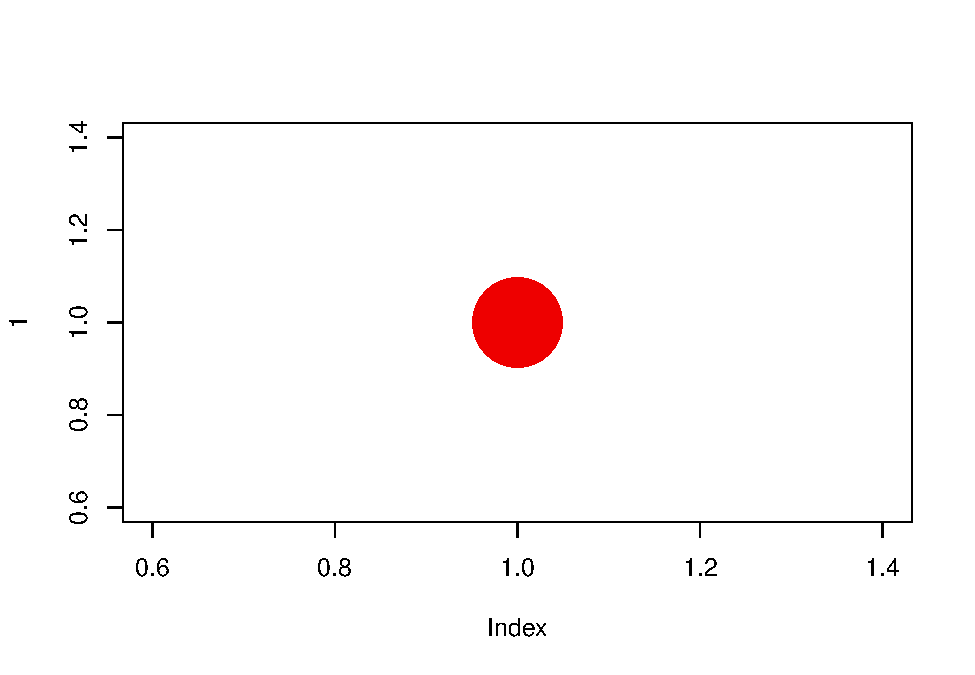
\includegraphics{02_The_R_language_files/figure-latex/unnamed-chunk-7-1.pdf}

This command creates a plot (graph), with only one point coloured by red. A hexadecimal color is specified with a \texttt{\#} and 2 digits for red, to digits for green and two digits for blue (\#RRGGBB). RR (red), GG (green) and BB (blue) are hexadecimal integers between 00 and FF specifying the intensity of the colour. For example, \texttt{\#0000FF} is displayed as blue, because the blue component is set to its highest value (FF) and the others are set to 00.

\hypertarget{integer}{%
\subsection{Integer}\label{integer}}

The next number type is the integer. Integer means the whole numbers, For example 4, 42 or -12. But in R we have to use the capital \texttt{L} suffix. \texttt{L} just indicates that this is a long, it's an internal storage type. It is a way to represent natural numbers like 1 and 2. Integers arise from counting, in most cases.

\begin{Shaded}
\begin{Highlighting}[]
\NormalTok{4L}
\CommentTok{\#\textgreater{} [1] 4}
\NormalTok{42L}
\CommentTok{\#\textgreater{} [1] 42}
\SpecialCharTok{{-}}\NormalTok{12L}
\CommentTok{\#\textgreater{} [1] {-}12}
\end{Highlighting}
\end{Shaded}

To sum it up, decimal values like \texttt{4.5} and whole numbers without \texttt{L} suffix are double in R. Whole numbers with \texttt{L} suffix are integers in R. Both double and integer are numerics.
Let's try something. Type in 2 and 2L, and execute them. You don't see the difference between the double 2 and the integer 2 from the output.

\begin{Shaded}
\begin{Highlighting}[]
\DecValTok{2}
\CommentTok{\#\textgreater{} [1] 2}
\NormalTok{2L}
\CommentTok{\#\textgreater{} [1] 2}
\end{Highlighting}
\end{Shaded}

However, there are two functions that reveal the difference. The \texttt{typeof()} and \texttt{class()} functions return almost the same values, the types of the data. Notice, the \texttt{class()} function with double argument returns \texttt{"numeric"}.

\begin{Shaded}
\begin{Highlighting}[]
\FunctionTok{typeof}\NormalTok{(}\DecValTok{2}\NormalTok{)}
\CommentTok{\#\textgreater{} [1] "double"}
\FunctionTok{typeof}\NormalTok{(2L)}
\CommentTok{\#\textgreater{} [1] "integer"}
\FunctionTok{class}\NormalTok{(}\DecValTok{2}\NormalTok{)}
\CommentTok{\#\textgreater{} [1] "numeric"}
\FunctionTok{class}\NormalTok{(2L)}
\CommentTok{\#\textgreater{} [1] "integer"}
\end{Highlighting}
\end{Shaded}

Of course, we can try these functions with decimal values.

\begin{Shaded}
\begin{Highlighting}[]
\FunctionTok{typeof}\NormalTok{(}\FloatTok{2.4}\NormalTok{)}
\CommentTok{\#\textgreater{} [1] "double"}
\FunctionTok{class}\NormalTok{(}\FloatTok{2.4}\NormalTok{)}
\CommentTok{\#\textgreater{} [1] "numeric"}
\end{Highlighting}
\end{Shaded}

\hypertarget{characters}{%
\subsection{Characters}\label{characters}}

Text (or string) values are called characters in R. For example type in some text inside quote marks.

\begin{Shaded}
\begin{Highlighting}[]
\StringTok{"some text"}
\CommentTok{\#\textgreater{} [1] "some text"}
\StringTok{\textquotesingle{}Dobó, István\textquotesingle{}}
\CommentTok{\#\textgreater{} [1] "Dobó, István"}
\StringTok{" sldjf odiuoiuoiu657676876987876875  32 23sdcsd)(/=(/\%"}
\CommentTok{\#\textgreater{} [1] " sldjf odiuoiuoiu657676876987876875  32 23sdcsd)(/=(/\%"}
\end{Highlighting}
\end{Shaded}

Note how the quotation marks in the editor indicate that \texttt{"some\ text"} is a string. Syntax highlighting also helps you to identify string values. It may also be noted that autocompletion is also working. We typed in only one quote mark, the second one appeared automatically. We can use double quote mark (\texttt{"}) and single quote mark (\texttt{\textquotesingle{}}), but the opening and the closing quote marks need to match. If we start with single quotation mark, we have to finish with single one. If we start with double quotation mark, we have to finish with double one.

We can use any characters inside quotation marks, except surrounding quotation marks.

Let's check out the \texttt{typeof()} and \texttt{class()} function with character data. They return \texttt{"character"}.

\begin{Shaded}
\begin{Highlighting}[]
\FunctionTok{typeof}\NormalTok{(}\StringTok{"Friday"}\NormalTok{)}
\CommentTok{\#\textgreater{} [1] "character"}
\FunctionTok{class}\NormalTok{(}\StringTok{"Friday"}\NormalTok{)}
\CommentTok{\#\textgreater{} [1] "character"}
\end{Highlighting}
\end{Shaded}

\hypertarget{logical}{%
\subsection{Logical}\label{logical}}

The last data types is the logical. Boolean values (TRUE or FALSE) are called logical in R. Let's head over to the script window and start with \texttt{TRUE}, in capital letters. \texttt{TRUE} is a logical. Logical constants can be either \texttt{TRUE} or \texttt{FALSE}.

\begin{Shaded}
\begin{Highlighting}[]
\ConstantTok{TRUE}
\CommentTok{\#\textgreater{} [1] TRUE}
\ConstantTok{FALSE}
\CommentTok{\#\textgreater{} [1] FALSE}
\end{Highlighting}
\end{Shaded}

\texttt{TRUE} and \texttt{FALSE} can be abbreviated to \texttt{T} and \texttt{F} respectively. However, I want to strongly encourage you to use the full versions, \texttt{TRUE} and \texttt{FALSE}.

\begin{Shaded}
\begin{Highlighting}[]
\NormalTok{T}
\CommentTok{\#\textgreater{} [1] TRUE}
\NormalTok{F}
\CommentTok{\#\textgreater{} [1] FALSE}
\end{Highlighting}
\end{Shaded}

Finally, we can check out the type these logical values.

\begin{Shaded}
\begin{Highlighting}[]
\FunctionTok{typeof}\NormalTok{(}\ConstantTok{TRUE}\NormalTok{)}
\CommentTok{\#\textgreater{} [1] "logical"}
\FunctionTok{class}\NormalTok{(F)}
\CommentTok{\#\textgreater{} [1] "logical"}
\end{Highlighting}
\end{Shaded}

Note, we did not use quotation marks in logical vales. If we use them, we will get character vales. For example:

\begin{Shaded}
\begin{Highlighting}[]
\FunctionTok{typeof}\NormalTok{(}\StringTok{"TRUE"}\NormalTok{)}
\CommentTok{\#\textgreater{} [1] "character"}
\end{Highlighting}
\end{Shaded}

To sum it up, R works with numerous data types. Some of the most basic types are double, integer, character and logical. We learned how to write \texttt{constants} in R. There are two functions \texttt{typeof()} and \texttt{class()} with which we can check out constants' type.

\hypertarget{operators}{%
\section{Operators}\label{operators}}

\hypertarget{arithmetic-operators}{%
\subsection{Arithmetic operators}\label{arithmetic-operators}}

In its most basic form, R can be used as a simple calculator. We can use the following arithmetic operators:

\begin{itemize}
\tightlist
\item
  Addition
\item
  Subtraction
\item
  Multiplication
\item
  Division
\item
  Exponentiation.
\end{itemize}

Let's put a basic addition, subtraction, multiplication, division and an extra expression, an exponentiation into our editor window. We use plus (\texttt{+}), minus (\texttt{-}), asterisk (\texttt{*}), slash (\texttt{/}) and double asterisks (\texttt{**}) or hat symbols (\texttt{\^{}}). Double asterisk \texttt{**} behaves exactly like \texttt{\^{}} (hat, caret), these are to-the-power-of, exponent operators.

\begin{Shaded}
\begin{Highlighting}[]
\FloatTok{34.1} \SpecialCharTok{+} \FloatTok{2e4} \CommentTok{\# Addition}
\CommentTok{\#\textgreater{} [1] 20034.1}
\DecValTok{0xe4} \SpecialCharTok{{-}} \DecValTok{23}  \CommentTok{\# Subtraction}
\CommentTok{\#\textgreater{} [1] 205}
\DecValTok{23} \SpecialCharTok{*} \DecValTok{45000} \CommentTok{\# Multiplication}
\CommentTok{\#\textgreater{} [1] 1035000}
\DecValTok{23}\SpecialCharTok{/}\DecValTok{12}      \CommentTok{\# Division}
\CommentTok{\#\textgreater{} [1] 1.916667}
\DecValTok{23} \SpecialCharTok{**} \DecValTok{12}   \CommentTok{\# Exponentiation}
\CommentTok{\#\textgreater{} [1] 2.191462e+16}
\DecValTok{23} \SpecialCharTok{\^{}} \DecValTok{12}    \CommentTok{\# Exponentiation}
\CommentTok{\#\textgreater{} [1] 2.191462e+16}
\end{Highlighting}
\end{Shaded}

Additionally, the modulo (\texttt{\%\%}) returns the remainder of the division of the number to the left by the number on its right, for example 5 modulo 3 or \texttt{5\ \%\%\ 3} is 2.

\begin{Shaded}
\begin{Highlighting}[]
\DecValTok{5} \SpecialCharTok{\%\%} \DecValTok{3}   \CommentTok{\# modulo: remainder of 5 divided by 3 }
\CommentTok{\#\textgreater{} [1] 2}
\end{Highlighting}
\end{Shaded}

The integer division \texttt{x\ \%/\%\ y} x divided by y but rounded down.

\begin{Shaded}
\begin{Highlighting}[]
\DecValTok{7} \SpecialCharTok{\%/\%} \DecValTok{3}   \CommentTok{\# integer division}
\CommentTok{\#\textgreater{} [1] 2}
\end{Highlighting}
\end{Shaded}

\hypertarget{logical-operators}{%
\subsection{Logical operators}\label{logical-operators}}

R uses standard logical notation for OR and AND, and NOT. First of all, the exclamation mark (\texttt{!}) stands for NOT. So if I type in \texttt{!TRUE}, I'll get false. Or surprisingly if I type in \texttt{!FALSE} I'll get true. It just inverts the value.

The ampersand (\texttt{\&}) is for AND. So I can type in \texttt{TRUE\ \&\ TRUE}, which means if true and true then I get true. If I type in \texttt{TRUE\ \&\ FALSE} then I'll receive false because both arguments have to be true in order for the result to be true.

Let's talk about the pipeline symbol (\texttt{\textbar{}}). The pipeline symbol means OR. So in this case I can type in \texttt{TRUE\ \textbar{}\ TRUE} and I'm going to get back true. If I type in \texttt{TRUE\ \textbar{}\ FALSE}, I'll get back true because for OR it is enough for only one value to be true to evaluate it as true.

\begin{Shaded}
\begin{Highlighting}[]
\SpecialCharTok{!}\ConstantTok{TRUE}
\CommentTok{\#\textgreater{} [1] FALSE}
\SpecialCharTok{!}\ConstantTok{FALSE}
\CommentTok{\#\textgreater{} [1] TRUE}
\ConstantTok{TRUE} \SpecialCharTok{\&} \ConstantTok{TRUE}
\CommentTok{\#\textgreater{} [1] TRUE}
\ConstantTok{TRUE} \SpecialCharTok{\&} \ConstantTok{FALSE}
\CommentTok{\#\textgreater{} [1] FALSE}
\ConstantTok{TRUE} \SpecialCharTok{|} \ConstantTok{TRUE}
\CommentTok{\#\textgreater{} [1] TRUE}
\ConstantTok{TRUE} \SpecialCharTok{|} \ConstantTok{FALSE}
\CommentTok{\#\textgreater{} [1] TRUE}
\end{Highlighting}
\end{Shaded}

\hypertarget{relational-operators}{%
\subsection{Relational operators}\label{relational-operators}}

Relational operators are used to compare between values. Here is a list of relational operators available in R.

\begin{longtable}[]{@{}ll@{}}
\toprule
\begin{minipage}[b]{(\columnwidth - 1\tabcolsep) * \real{0.17}}\raggedright
Operator\strut
\end{minipage} & \begin{minipage}[b]{(\columnwidth - 1\tabcolsep) * \real{0.36}}\raggedright
Description\strut
\end{minipage}\tabularnewline
\midrule
\endhead
\begin{minipage}[t]{(\columnwidth - 1\tabcolsep) * \real{0.17}}\raggedright
\texttt{\textless{}}\strut
\end{minipage} & \begin{minipage}[t]{(\columnwidth - 1\tabcolsep) * \real{0.36}}\raggedright
Less than\strut
\end{minipage}\tabularnewline
\begin{minipage}[t]{(\columnwidth - 1\tabcolsep) * \real{0.17}}\raggedright
\texttt{\textgreater{}}\strut
\end{minipage} & \begin{minipage}[t]{(\columnwidth - 1\tabcolsep) * \real{0.36}}\raggedright
Greater than\strut
\end{minipage}\tabularnewline
\begin{minipage}[t]{(\columnwidth - 1\tabcolsep) * \real{0.17}}\raggedright
\texttt{\textless{}=}\strut
\end{minipage} & \begin{minipage}[t]{(\columnwidth - 1\tabcolsep) * \real{0.36}}\raggedright
Less than or equal to\strut
\end{minipage}\tabularnewline
\begin{minipage}[t]{(\columnwidth - 1\tabcolsep) * \real{0.17}}\raggedright
\texttt{\textgreater{}=}\strut
\end{minipage} & \begin{minipage}[t]{(\columnwidth - 1\tabcolsep) * \real{0.36}}\raggedright
Greater than or equal to\strut
\end{minipage}\tabularnewline
\begin{minipage}[t]{(\columnwidth - 1\tabcolsep) * \real{0.17}}\raggedright
\texttt{==}\strut
\end{minipage} & \begin{minipage}[t]{(\columnwidth - 1\tabcolsep) * \real{0.36}}\raggedright
Equal to\strut
\end{minipage}\tabularnewline
\begin{minipage}[t]{(\columnwidth - 1\tabcolsep) * \real{0.17}}\raggedright
\texttt{!=}\strut
\end{minipage} & \begin{minipage}[t]{(\columnwidth - 1\tabcolsep) * \real{0.36}}\raggedright
Not equal to\strut
\end{minipage}\tabularnewline
\bottomrule
\end{longtable}

\begin{Shaded}
\begin{Highlighting}[]
\DecValTok{2} \SpecialCharTok{\textless{}} \FloatTok{2.3}
\CommentTok{\#\textgreater{} [1] TRUE}
\DecValTok{2} \SpecialCharTok{\textless{}=} \FloatTok{2.3}
\CommentTok{\#\textgreater{} [1] TRUE}
\DecValTok{2} \SpecialCharTok{\textgreater{}} \FloatTok{2.3}
\CommentTok{\#\textgreater{} [1] FALSE}
\DecValTok{2} \SpecialCharTok{\textgreater{}=} \FloatTok{2.3}
\CommentTok{\#\textgreater{} [1] FALSE}
\DecValTok{2} \SpecialCharTok{==} \FloatTok{2.3}
\CommentTok{\#\textgreater{} [1] FALSE}
\DecValTok{2} \SpecialCharTok{!=} \FloatTok{2.3}
\CommentTok{\#\textgreater{} [1] TRUE}

\StringTok{"apple"} \SpecialCharTok{==} \StringTok{"Apple"}
\CommentTok{\#\textgreater{} [1] FALSE}
\StringTok{"apple"} \SpecialCharTok{!=} \StringTok{"Apple"}
\CommentTok{\#\textgreater{} [1] TRUE}

\ConstantTok{TRUE} \SpecialCharTok{==} \ConstantTok{FALSE}
\CommentTok{\#\textgreater{} [1] FALSE}
\ConstantTok{TRUE} \SpecialCharTok{!=} \ConstantTok{FALSE}
\CommentTok{\#\textgreater{} [1] TRUE}

\ConstantTok{TRUE} \SpecialCharTok{==} \DecValTok{1}
\CommentTok{\#\textgreater{} [1] TRUE}
\ConstantTok{TRUE} \SpecialCharTok{!=} \DecValTok{1}
\CommentTok{\#\textgreater{} [1] FALSE}

\NormalTok{(}\SpecialCharTok{{-}}\DecValTok{6} \SpecialCharTok{*} \DecValTok{14}\NormalTok{) }\SpecialCharTok{==}\NormalTok{ (}\DecValTok{17} \SpecialCharTok{{-}} \DecValTok{101}\NormalTok{)}
\CommentTok{\#\textgreater{} [1] TRUE}
\end{Highlighting}
\end{Shaded}

The result of comparison is a Boolean value (\texttt{TRUE} or \texttt{FALSE}).

\hypertarget{assignment-operators}{%
\subsection{Assignment operators}\label{assignment-operators}}

We will use one of them, the ``left arrow'' (\texttt{\textless{}-}) operator. The ``left arrow'' assignment operator is actually two symbols, a „less than'' sign and a „minus''. Good to know, there is a shortcut for assignment operator, namely Alt+- in \emph{RStudio}. What is the assignment operator for? It is for \emph{objects}. Objects allow you to store a value in R. You can then later use this object's name to easily access the value that is stored within this object.

Let's create our first object. You can assign the value 4 to an object \texttt{my\_object} with the command:

\begin{Shaded}
\begin{Highlighting}[]
\NormalTok{my\_object }\OtherTok{\textless{}{-}} \DecValTok{4}
\end{Highlighting}
\end{Shaded}

Then type in the name of the object my\_object, and execute it. Notice that when you ask R to print my\_object, the value 4 appears.

\begin{Shaded}
\begin{Highlighting}[]
\NormalTok{my\_object}
\CommentTok{\#\textgreater{} [1] 4}
\end{Highlighting}
\end{Shaded}

If we use \texttt{class()} or \texttt{typeof()} functions, we'll get type of the object.

\begin{Shaded}
\begin{Highlighting}[]
\FunctionTok{typeof}\NormalTok{(my\_object)}
\CommentTok{\#\textgreater{} [1] "double"}
\FunctionTok{class}\NormalTok{(my\_object)}
\CommentTok{\#\textgreater{} [1] "numeric"}
\end{Highlighting}
\end{Shaded}

\hypertarget{miscellaneous-operators}{%
\subsection{Miscellaneous operators}\label{miscellaneous-operators}}

These operators are used to for specific purpose and not general mathematical or logical computation.

Colon operator (\texttt{:}) creates the series of numbers in sequence for a vector.

\begin{Shaded}
\begin{Highlighting}[]
\DecValTok{2}\SpecialCharTok{:}\DecValTok{8}
\CommentTok{\#\textgreater{} [1] 2 3 4 5 6 7 8}
\end{Highlighting}
\end{Shaded}

The \texttt{\%in\%} operator is used to identify if an element belongs to a vector. It returns a logical vector indicating if there is a match or not for all elements in the left operand in the right operand.

\begin{Shaded}
\begin{Highlighting}[]
\FunctionTok{c}\NormalTok{(}\DecValTok{3}\NormalTok{, }\DecValTok{4}\NormalTok{, }\DecValTok{5}\NormalTok{, }\DecValTok{7}\NormalTok{, }\DecValTok{10}\NormalTok{) }\SpecialCharTok{\%in\%} \FunctionTok{c}\NormalTok{(}\DecValTok{2}\NormalTok{, }\DecValTok{4}\NormalTok{, }\DecValTok{6}\NormalTok{, }\DecValTok{8}\NormalTok{, }\DecValTok{10}\NormalTok{)}
\CommentTok{\#\textgreater{} [1] FALSE  TRUE FALSE FALSE  TRUE}
\end{Highlighting}
\end{Shaded}

The double colon operator (\texttt{::}) is a binary operator to access functions or datasets from packages. As we mentioned, packages extend R's knowledge. Every R package contains functions and/or dataset. Every R package has a name. For example we have an installed packages called \textbf{MASS}. In \textbf{MASS} packages, there is dataset called \texttt{survey}. So, we can type in \texttt{MASS::survey}, to reach the survey dataset from \textbf{MASS} package.

\begin{Shaded}
\begin{Highlighting}[]
\FunctionTok{str}\NormalTok{(MASS}\SpecialCharTok{::}\NormalTok{survey)}
\CommentTok{\#\textgreater{} \textquotesingle{}data.frame\textquotesingle{}:    237 obs. of  12 variables:}
\CommentTok{\#\textgreater{}  $ Sex   : Factor w/ 2 levels "Female","Male": 1 2 2 2 2 1 2 1 2 2 ...}
\CommentTok{\#\textgreater{}  $ Wr.Hnd: num  18.5 19.5 18 18.8 20 18 17.7 17 20 18.5 ...}
\CommentTok{\#\textgreater{}  $ NW.Hnd: num  18 20.5 13.3 18.9 20 17.7 17.7 17.3 19.5 18.5 ...}
\CommentTok{\#\textgreater{}  $ W.Hnd : Factor w/ 2 levels "Left","Right": 2 1 2 2 2 2 2 2 2 2 ...}
\CommentTok{\#\textgreater{}  $ Fold  : Factor w/ 3 levels "L on R","Neither",..: 3 3 1 3 2 1 1 3 3 3 ...}
\CommentTok{\#\textgreater{}  $ Pulse : int  92 104 87 NA 35 64 83 74 72 90 ...}
\CommentTok{\#\textgreater{}  $ Clap  : Factor w/ 3 levels "Left","Neither",..: 1 1 2 2 3 3 3 3 3 3 ...}
\CommentTok{\#\textgreater{}  $ Exer  : Factor w/ 3 levels "Freq","None",..: 3 2 2 2 3 3 1 1 3 3 ...}
\CommentTok{\#\textgreater{}  $ Smoke : Factor w/ 4 levels "Heavy","Never",..: 2 4 3 2 2 2 2 2 2 2 ...}
\CommentTok{\#\textgreater{}  $ Height: num  173 178 NA 160 165 ...}
\CommentTok{\#\textgreater{}  $ M.I   : Factor w/ 2 levels "Imperial","Metric": 2 1 NA 2 2 1 1 2 2 2 ...}
\CommentTok{\#\textgreater{}  $ Age   : num  18.2 17.6 16.9 20.3 23.7 ...}
\end{Highlighting}
\end{Shaded}

\hypertarget{operator-precedence-in-r}{%
\subsection{Operator Precedence in R}\label{operator-precedence-in-r}}

As we mentioned, R can be used as a powerful calculator. Simply type an arithmetic expression and press Ctrl+Enter.

\begin{Shaded}
\begin{Highlighting}[]
\DecValTok{4} \SpecialCharTok{+} \DecValTok{8}       \CommentTok{\# will return the result 12}
\CommentTok{\#\textgreater{} [1] 12}
\DecValTok{4} \SpecialCharTok{+} \DecValTok{5} \SpecialCharTok{+} \DecValTok{3}   \CommentTok{\# will return the result 12}
\CommentTok{\#\textgreater{} [1] 12}
\end{Highlighting}
\end{Shaded}

But, there could be problems if you are not careful. R normally execute your arithmetic expression by evaluating each item from left to right. 4 plus 8 equals 12. 4 plus 5 plus 3 equals twelve. But good to know, operators have precedence in the order of evaluation.

Let's start with more complex expressions that can cause problems if you are not careful.

\begin{Shaded}
\begin{Highlighting}[]
\DecValTok{4} \SpecialCharTok{+} \DecValTok{5} \SpecialCharTok{*} \DecValTok{3}    \CommentTok{\# will return the result 19}
\CommentTok{\#\textgreater{} [1] 19}
\end{Highlighting}
\end{Shaded}

Notice that the expression was not evaluated strictly left to right. R actually evaluated 5 times 3 and then added that result to 4. The R operator precedence rules caused this result.

Multiplication and division have a higher precedence than the addition and subtraction operator so the multiplication is performed before the addition. We can arrange the operators in order from high precedence to low precedence. We can extend the list with exponentiation.

Operators with higher precedence (nearer top of the list) are performed before those with lower precedence (nearer to the bottom).

\begin{longtable}[]{@{}ll@{}}
\toprule
Operator & Description\tabularnewline
\midrule
\endhead
\texttt{::} & access\tabularnewline
\texttt{\$} & component\tabularnewline
\texttt{{[}} \texttt{{[}{[}} & indexing\tabularnewline
\texttt{\^{}} \texttt{**} & exponentiation\tabularnewline
\texttt{-} \texttt{+} & unary minus, unary plus\tabularnewline
\texttt{:} & sequence operator\tabularnewline
\texttt{\%any\%} e.g.~\texttt{\%\%} \texttt{\%/\%} \texttt{\%in\%} & special operators\tabularnewline
\texttt{*} \texttt{/} & multiplication, division\tabularnewline
\texttt{+} \texttt{-} & addition, subtraction\tabularnewline
\texttt{\textless{}} \texttt{\textgreater{}} \texttt{\textless{}=} \texttt{\textgreater{}=} \texttt{==} \texttt{!=} & comparisions\tabularnewline
\texttt{!} & logical NOT\tabularnewline
\texttt{\&} & logical AND\tabularnewline
\texttt{\textbar{}} & logical OR\tabularnewline
\texttt{\textless{}-} & assignment\tabularnewline
\bottomrule
\end{longtable}

The exponentiation operator has a higher precedence than the multiplication, so the the exponentiation is the first that performed. Three squared multiplied by two:

\begin{Shaded}
\begin{Highlighting}[]
\DecValTok{2} \SpecialCharTok{*} \DecValTok{3} \SpecialCharTok{**} \DecValTok{2}
\CommentTok{\#\textgreater{} [1] 18}
\end{Highlighting}
\end{Shaded}

Operator precedence can be overridden with explicit use of parentheses. In the case of this example, we could enter

\begin{Shaded}
\begin{Highlighting}[]
\NormalTok{(}\DecValTok{4} \SpecialCharTok{+} \DecValTok{5}\NormalTok{) }\SpecialCharTok{*} \DecValTok{3} 
\CommentTok{\#\textgreater{} [1] 27}
\NormalTok{(}\DecValTok{2} \SpecialCharTok{*} \DecValTok{3}\NormalTok{) }\SpecialCharTok{**} \DecValTok{2}
\CommentTok{\#\textgreater{} [1] 36}
\end{Highlighting}
\end{Shaded}

In practise, if you are at all unsure about the precedence of your operators, the simplest thing to do is to use parentheses to make the evaluation order explicit.

\hypertarget{binary-and-unary-operators}{%
\subsection{Binary and unary operators}\label{binary-and-unary-operators}}

Another thing about operators. There are two different type of operators. Binary and unary operators. The question is, how many operands they require to work properly.

A unary operator is an operator that operates on only one operand. Binary operators that we used earlier operates two operands. We've talked about binary operators so far. Addition, subtraction, multiplication, division, exponentiation are binary operators. They require two operands to work properly.

For example \texttt{5\ –} (select these characters for executing) is wrong, we get a continuation prompt. We could complete the command. but we never do that. Click on console pane, and hit Esc.

Complete the line in the script editor, \texttt{5–2}, hit Ctrl+Enter equals 3. Subtraction is a binary operator, it has two operands. Five and two.

In R, there are a few unary operators, for example unary minus, and unary plus. They are the sign operators. They are used to indicate or change the sign of a value. The \texttt{+} and \texttt{-} signs indicate the sign of a value. The plus sign can be used to signal that we have a positive number. It can be omitted and it is mostly done so. We could type \texttt{5}, \texttt{+5}. The minus sign changes the sign of a value. To write negative five, we need type in \texttt{-5}. This is the unary minus operator.

\begin{Shaded}
\begin{Highlighting}[]
\DecValTok{5}
\CommentTok{\#\textgreater{} [1] 5}
\SpecialCharTok{+}\DecValTok{5}
\CommentTok{\#\textgreater{} [1] 5}
\SpecialCharTok{{-}}\DecValTok{5}
\CommentTok{\#\textgreater{} [1] {-}5}
\end{Highlighting}
\end{Shaded}

To sum up, we really need another list in the script editor. R Terminology.
We talked about constants, this is a language element which has fix value, we can not change. 5 means five, Friday in quotes means Friday. TRUE means logical TRUE. Operators perform mathematical or logical operations on values, on constants. Operators have precedence and operators can be unary or binary. Every constant has a basic type (double, integer, character, logical). And, we can build expressions with constants, operators and parentheses.
We also talked about comment in R, that is everything after a \# (a hashtag). It will have no effect if you run it in R.

\hypertarget{objects}{%
\section{Objects}\label{objects}}

We talked about object that is very important language element in R. We will be discussing everything that needs to be known about objects and data structures.

Lets' start with objects. An object allows you to store data in R for later use. Suppose the height of a rectangle is 2. Let's assign this value 2 to an object. Let's call it \texttt{height}.

\begin{Shaded}
\begin{Highlighting}[]
\NormalTok{height }\OtherTok{\textless{}{-}} \DecValTok{2}
\end{Highlighting}
\end{Shaded}

This time, R does not print anything in the console, but we can not see error messages either. Command executing without error messages, even without any messages indicates everything is ok. The command evaluated successfully. Look at the top right pane. In the environment tab we have a new item in the list. \texttt{Height} and its value 2. All objects with name and value will appear in this list. We have only one object in this session, so this list has only one item.

If you now simply type and execute height in the script window, R returns 2.

\begin{Shaded}
\begin{Highlighting}[]
\NormalTok{height}
\CommentTok{\#\textgreater{} [1] 2}
\end{Highlighting}
\end{Shaded}

We can do a similar thing for the width of our imaginary rectangle. We assign the value 4 to an object called \texttt{width}.

\begin{Shaded}
\begin{Highlighting}[]
\NormalTok{width }\OtherTok{\textless{}{-}} \DecValTok{4}
\end{Highlighting}
\end{Shaded}

In the top right pane, we have two items in the list. Actually, this list in the environment tab shows the \emph{workspace}. Workspace is a special location in your computer's memory that temporarily stores data we just created using R.
Workspace is the place where R objects `live'. You can list all objects with the \texttt{ls()} function.

\begin{Shaded}
\begin{Highlighting}[]
\FunctionTok{ls}\NormalTok{()}
\CommentTok{\#\textgreater{} [1] "height"    "my\_object" "width"}
\end{Highlighting}
\end{Shaded}

This shows you a list of all the objects you have created up to now. There are two objects in your workspace at the moment, \texttt{height} and \texttt{width}. If we try to access object that's not in the workspace, \texttt{depth} for example, R throws an error.

\begin{Shaded}
\begin{Highlighting}[]
\NormalTok{depth  }\CommentTok{\# error}
\end{Highlighting}
\end{Shaded}

Suppose you now want to find out the area of our imaginary rectangle, which is height multiplied by width. Height equals 2, and width equals 4, so the result is 8. We have two ways to calculate the area:

\begin{Shaded}
\begin{Highlighting}[]
\DecValTok{2} \SpecialCharTok{*} \DecValTok{4}
\CommentTok{\#\textgreater{} [1] 8}
\NormalTok{height }\SpecialCharTok{*}\NormalTok{ width}
\CommentTok{\#\textgreater{} [1] 8}
\end{Highlighting}
\end{Shaded}

The second line with objects is more advanced than the first line with constants. Let's also assign this result to a new object, called area.

\begin{Shaded}
\begin{Highlighting}[]
\NormalTok{area }\OtherTok{\textless{}{-}}\NormalTok{ height }\SpecialCharTok{*}\NormalTok{ width}
\NormalTok{area }
\CommentTok{\#\textgreater{} [1] 8}
\end{Highlighting}
\end{Shaded}

We can print the value of object \texttt{area}, type and execute \texttt{area}. It's 8. Inspecting the workspace again with \texttt{ls()}, shows that the workspace contains three objects now: \texttt{area}, \texttt{height} and \texttt{width}.

Now, this is all great, but what if you want to recalculate the area of your imaginary rectangle when the height is 3 and the width is 6? You'd have to reassign the objects width and height in the script window, and then recalculate the area. The value of area will change, executing area will return 18.

\begin{Shaded}
\begin{Highlighting}[]
\NormalTok{height }\OtherTok{\textless{}{-}} \DecValTok{3}
\NormalTok{width }\OtherTok{\textless{}{-}} \DecValTok{6}
\NormalTok{area }\OtherTok{\textless{}{-}}\NormalTok{ height }\SpecialCharTok{*}\NormalTok{ width}
\NormalTok{area }
\CommentTok{\#\textgreater{} [1] 18}
\end{Highlighting}
\end{Shaded}

How to find the perimeter of this rectangle. Let's create a new object called perimeter.

\begin{Shaded}
\begin{Highlighting}[]
\NormalTok{perimeter }\OtherTok{\textless{}{-}} \DecValTok{2}\SpecialCharTok{*}\NormalTok{(width}\SpecialCharTok{+}\NormalTok{height)}
\NormalTok{perimeter}
\CommentTok{\#\textgreater{} [1] 18}
\end{Highlighting}
\end{Shaded}

Let's sum up the objects. The general form of creating or modifying an object is object name, assignment operator and an expression.

\begin{Shaded}
\begin{Highlighting}[]
\NormalTok{object\_name }\OtherTok{\textless{}{-}}\NormalTok{ expression}
\end{Highlighting}
\end{Shaded}

First, we have to choose a valid object name. Object name can contain any letters from English alphabet, underscore, dot, or digit. We need to start with letter in an object name. Expression can be a simply constant, or an object name, or constant and object names with operators and parentheses.

We can create logical object or double object, integer object and character object:

\begin{Shaded}
\begin{Highlighting}[]
\NormalTok{x.logical }\OtherTok{\textless{}{-}} \ConstantTok{TRUE}
\NormalTok{y.double }\OtherTok{\textless{}{-}} \FloatTok{12.3}
\NormalTok{z.integer }\OtherTok{\textless{}{-}}\NormalTok{ 12L}
\NormalTok{k.character }\OtherTok{\textless{}{-}} \StringTok{"Hello world!"}
\end{Highlighting}
\end{Shaded}

and we can print their type, with \texttt{typeof()} or \texttt{class()} function.

\begin{Shaded}
\begin{Highlighting}[]
\FunctionTok{typeof}\NormalTok{(x.logical)}
\CommentTok{\#\textgreater{} [1] "logical"}
\FunctionTok{class}\NormalTok{(x.logical)}
\CommentTok{\#\textgreater{} [1] "logical"}

\FunctionTok{typeof}\NormalTok{(y.double)}
\CommentTok{\#\textgreater{} [1] "double"}
\FunctionTok{class}\NormalTok{(y.double)}
\CommentTok{\#\textgreater{} [1] "numeric"}

\FunctionTok{typeof}\NormalTok{(z.integer)}
\CommentTok{\#\textgreater{} [1] "integer"}
\FunctionTok{class}\NormalTok{(z.integer)}
\CommentTok{\#\textgreater{} [1] "integer"}

\FunctionTok{typeof}\NormalTok{(k.character)}
\CommentTok{\#\textgreater{} [1] "character"}
\FunctionTok{class}\NormalTok{(k.character)}
\CommentTok{\#\textgreater{} [1] "character"}
\end{Highlighting}
\end{Shaded}

\hypertarget{testing-the-type}{%
\subsection{Testing the type}\label{testing-the-type}}

Instead of asking for the type or class of an object, you can also use the is-dot-functions to see whether objects are actually of a certain type. To see if an object is a double, we can use the \texttt{is.double()} function. It returns a logical value. \texttt{TRUE} or \texttt{FALSE}. To see if an object is integer, we can use \texttt{is.integer()}. There is \texttt{is.numeric()} function to see whether objects are numeric. The integer and double are numerics. Let's try the \texttt{is.logical()} and the \texttt{is.character()} functions.

\begin{Shaded}
\begin{Highlighting}[]
\CommentTok{\# is.*() functions, test of types}
\FunctionTok{is.double}\NormalTok{(x.logical)}
\CommentTok{\#\textgreater{} [1] FALSE}
\FunctionTok{is.double}\NormalTok{(y.double)}
\CommentTok{\#\textgreater{} [1] TRUE}
\FunctionTok{is.double}\NormalTok{(z.integer)}
\CommentTok{\#\textgreater{} [1] FALSE}
\FunctionTok{is.double}\NormalTok{(k.character)}
\CommentTok{\#\textgreater{} [1] FALSE}

\FunctionTok{is.integer}\NormalTok{(x.logical)}
\CommentTok{\#\textgreater{} [1] FALSE}
\FunctionTok{is.integer}\NormalTok{(y.double)}
\CommentTok{\#\textgreater{} [1] FALSE}
\FunctionTok{is.integer}\NormalTok{(z.integer)}
\CommentTok{\#\textgreater{} [1] TRUE}
\FunctionTok{is.integer}\NormalTok{(k.character)}
\CommentTok{\#\textgreater{} [1] FALSE}

\FunctionTok{is.numeric}\NormalTok{(x.logical)}
\CommentTok{\#\textgreater{} [1] FALSE}
\FunctionTok{is.numeric}\NormalTok{(y.double)}
\CommentTok{\#\textgreater{} [1] TRUE}
\FunctionTok{is.numeric}\NormalTok{(z.integer)}
\CommentTok{\#\textgreater{} [1] TRUE}
\FunctionTok{is.numeric}\NormalTok{(k.character)}
\CommentTok{\#\textgreater{} [1] FALSE}

\FunctionTok{is.logical}\NormalTok{(x.logical)}
\CommentTok{\#\textgreater{} [1] TRUE}
\FunctionTok{is.logical}\NormalTok{(y.double)}
\CommentTok{\#\textgreater{} [1] FALSE}
\FunctionTok{is.logical}\NormalTok{(z.integer)}
\CommentTok{\#\textgreater{} [1] FALSE}
\FunctionTok{is.logical}\NormalTok{(k.character)}
\CommentTok{\#\textgreater{} [1] FALSE}

\FunctionTok{is.character}\NormalTok{(x.logical)}
\CommentTok{\#\textgreater{} [1] FALSE}
\FunctionTok{is.character}\NormalTok{(y.double)}
\CommentTok{\#\textgreater{} [1] FALSE}
\FunctionTok{is.character}\NormalTok{(z.integer)}
\CommentTok{\#\textgreater{} [1] FALSE}
\FunctionTok{is.character}\NormalTok{(k.character)}
\CommentTok{\#\textgreater{} [1] TRUE}
\end{Highlighting}
\end{Shaded}

\hypertarget{coercion}{%
\subsection{Coercion}\label{coercion}}

There are cases in which you want to change the type of an object to another one. How would that work? This is where coercion comes into play! By using the as-dot-functions one can coerce the type of a variable to another type. Many ways of transformation between types are possible. Have a look at these examples.

\begin{Shaded}
\begin{Highlighting}[]
\CommentTok{\# as.*() functions, coercion}
\FunctionTok{as.logical}\NormalTok{(y.double)}
\CommentTok{\#\textgreater{} [1] TRUE}
\FunctionTok{as.logical}\NormalTok{(z.integer)}
\CommentTok{\#\textgreater{} [1] TRUE}
\FunctionTok{as.logical}\NormalTok{(k.character)}
\CommentTok{\#\textgreater{} [1] NA}
\end{Highlighting}
\end{Shaded}

The first three commands here coerce three different objects to a logical. Every number except zero coerced to TRUE, so the first two commands return TRUE. The third command outputs an NA, a missing value. R doesn't understand how to transform ``Hello world'' into a logical, and decides to return a Not Available instead.
We can try to convert zero to logical.

\begin{Shaded}
\begin{Highlighting}[]
\FunctionTok{as.logical}\NormalTok{(}\DecValTok{0}\NormalTok{)}
\CommentTok{\#\textgreater{} [1] FALSE}
\end{Highlighting}
\end{Shaded}

The result is \texttt{FALSE}. We can easily coerce logical, integer and double to character.

\begin{Shaded}
\begin{Highlighting}[]
\FunctionTok{as.character}\NormalTok{(y.double)}
\CommentTok{\#\textgreater{} [1] "12.3"}
\FunctionTok{as.character}\NormalTok{(z.integer)}
\CommentTok{\#\textgreater{} [1] "12"}
\FunctionTok{as.character}\NormalTok{(x.logical)}
\CommentTok{\#\textgreater{} [1] "TRUE"}
\end{Highlighting}
\end{Shaded}

Let's try to find out how to convert logical and character to number? What functions we have in R with which we can achieve this? Yes, \texttt{as.double()}, \texttt{as.integer()} and \texttt{as.numeric()}. \texttt{as.numeric()} is identical to \texttt{as.double()}.

\begin{Shaded}
\begin{Highlighting}[]
\FunctionTok{as.double}\NormalTok{(x.logical)}
\CommentTok{\#\textgreater{} [1] 1}
\FunctionTok{as.double}\NormalTok{(z.integer)}
\CommentTok{\#\textgreater{} [1] 12}
\FunctionTok{as.double}\NormalTok{(k.character)}
\CommentTok{\#\textgreater{} [1] NA}

\FunctionTok{as.integer}\NormalTok{(y.double)}
\CommentTok{\#\textgreater{} [1] 12}
\FunctionTok{as.integer}\NormalTok{(x.logical)}
\CommentTok{\#\textgreater{} [1] 1}
\FunctionTok{as.integer}\NormalTok{(k.character)}
\CommentTok{\#\textgreater{} [1] NA}

\FunctionTok{as.numeric}\NormalTok{(x.logical)}
\CommentTok{\#\textgreater{} [1] 1}
\FunctionTok{as.numeric}\NormalTok{(y.double)}
\CommentTok{\#\textgreater{} [1] 12.3}
\FunctionTok{as.numeric}\NormalTok{(z.integer)}
\CommentTok{\#\textgreater{} [1] 12}
\FunctionTok{as.numeric}\NormalTok{(k.character)}
\CommentTok{\#\textgreater{} [1] NA}
\end{Highlighting}
\end{Shaded}

Logical TRUE coerces to the numeric one (1). FALSE, however, coerces to the numeric zero (0). Valid number in a string coerces to number, invalid number in a string, for example ``hello'', coerces missing value. R doesn't understand how to transform ``hello'' into a numeric, and decides to return a Not Available (NA) instead.

\begin{Shaded}
\begin{Highlighting}[]
\FunctionTok{as.double}\NormalTok{(}\ConstantTok{TRUE}\NormalTok{)}
\CommentTok{\#\textgreater{} [1] 1}
\FunctionTok{as.numeric}\NormalTok{(}\ConstantTok{TRUE}\NormalTok{)}
\CommentTok{\#\textgreater{} [1] 1}
\FunctionTok{as.integer}\NormalTok{(}\ConstantTok{TRUE}\NormalTok{)}
\CommentTok{\#\textgreater{} [1] 1}

\FunctionTok{as.double}\NormalTok{(}\ConstantTok{FALSE}\NormalTok{)}
\CommentTok{\#\textgreater{} [1] 0}
\FunctionTok{as.numeric}\NormalTok{(}\ConstantTok{FALSE}\NormalTok{)}
\CommentTok{\#\textgreater{} [1] 0}
\FunctionTok{as.integer}\NormalTok{(}\ConstantTok{FALSE}\NormalTok{)}
\CommentTok{\#\textgreater{} [1] 0}

\FunctionTok{as.double}\NormalTok{(}\StringTok{"12.3"}\NormalTok{)}
\CommentTok{\#\textgreater{} [1] 12.3}
\FunctionTok{as.numeric}\NormalTok{(}\StringTok{"12.3"}\NormalTok{)}
\CommentTok{\#\textgreater{} [1] 12.3}
\FunctionTok{as.integer}\NormalTok{(}\StringTok{"12.3"}\NormalTok{)}
\CommentTok{\#\textgreater{} [1] 12}

\FunctionTok{as.double}\NormalTok{(}\StringTok{"hello"}\NormalTok{)}
\CommentTok{\#\textgreater{} [1] NA}
\FunctionTok{as.numeric}\NormalTok{(}\StringTok{"hello"}\NormalTok{)}
\CommentTok{\#\textgreater{} [1] NA}
\FunctionTok{as.integer}\NormalTok{(}\StringTok{"hello"}\NormalTok{)}
\CommentTok{\#\textgreater{} [1] NA}
\end{Highlighting}
\end{Shaded}

\hypertarget{data-structures}{%
\section{Data structures}\label{data-structures}}

\hypertarget{vectors}{%
\subsection{Vectors}\label{vectors}}

In R, we use data sets all the time. Data sets are a collection or group of values, double, integer, character or logical values. They are the result of a scientific measurements, a surveys or other data collection methods. For example, you may record the ages of each member of your family. In R, we have to use the \texttt{c()} function for this, which allows you to combine values into a vector. This is a four member family, 2 children, mother, father. We could combine the ages of each member of family. Execute this command.

\begin{Shaded}
\begin{Highlighting}[]
\FunctionTok{c}\NormalTok{(}\DecValTok{18}\NormalTok{, }\DecValTok{20}\NormalTok{, }\DecValTok{47}\NormalTok{, }\DecValTok{49}\NormalTok{)}
\CommentTok{\#\textgreater{} [1] 18 20 47 49}
\end{Highlighting}
\end{Shaded}

As you can see in the output, it is a vector. A vector is nothing more than a sequence of data elements of the same basic data type. This is a double vector. We can check it with \texttt{typeof()} or \texttt{is.double()} functions.

\begin{Shaded}
\begin{Highlighting}[]
\FunctionTok{typeof}\NormalTok{(}\FunctionTok{c}\NormalTok{(}\DecValTok{18}\NormalTok{, }\DecValTok{20}\NormalTok{, }\DecValTok{47}\NormalTok{, }\DecValTok{49}\NormalTok{))}
\CommentTok{\#\textgreater{} [1] "double"}
\FunctionTok{is.double}\NormalTok{(}\FunctionTok{c}\NormalTok{(}\DecValTok{18}\NormalTok{, }\DecValTok{20}\NormalTok{, }\DecValTok{47}\NormalTok{, }\DecValTok{49}\NormalTok{))}
\CommentTok{\#\textgreater{} [1] TRUE}
\end{Highlighting}
\end{Shaded}

Of course we could also assign this double vector to a new object, \texttt{age} for example.

\begin{Shaded}
\begin{Highlighting}[]
\NormalTok{age }\OtherTok{\textless{}{-}} \FunctionTok{c}\NormalTok{(}\DecValTok{18}\NormalTok{, }\DecValTok{20}\NormalTok{, }\DecValTok{47}\NormalTok{, }\DecValTok{49}\NormalTok{)}
\end{Highlighting}
\end{Shaded}

We can assert that it is a vector, by typing

\begin{Shaded}
\begin{Highlighting}[]
\FunctionTok{is.vector}\NormalTok{(age)}
\CommentTok{\#\textgreater{} [1] TRUE}
\end{Highlighting}
\end{Shaded}

We can also check the top right pane, the workspace. Age is listed, and we can see, it is a double vector indicated by num with four elements. ``Num'' means double.

We can print the value of this vector.

\begin{Shaded}
\begin{Highlighting}[]
\NormalTok{age}
\CommentTok{\#\textgreater{} [1] 18 20 47 49}
\end{Highlighting}
\end{Shaded}

Please execute the \texttt{age} command. We can see, \texttt{age} contains four elements. The firs element is 18, the second 20, the third is 47, and the last element is 49. Every vector is a sequence of data elements. We can check the length of this vector with \texttt{length()} function.

\begin{Shaded}
\begin{Highlighting}[]
\FunctionTok{length}\NormalTok{(age)}
\CommentTok{\#\textgreater{} [1] 4}
\end{Highlighting}
\end{Shaded}

It tells us, \texttt{age} vector holds four elements. The length of this vector is 4.

Good to know, the vector is the simplest data structure in R. Objects we've created in the previous topic, are also vectors. They're all just vectors of length 1. They contain a single number (for example object \texttt{height}) or a single character, object \texttt{k.character}. We can check this with \texttt{is.vector()} function.

\begin{Shaded}
\begin{Highlighting}[]
\FunctionTok{is.vector}\NormalTok{(height)}
\CommentTok{\#\textgreater{} [1] TRUE}
\FunctionTok{is.vector}\NormalTok{(k.character)}
\CommentTok{\#\textgreater{} [1] TRUE}
\end{Highlighting}
\end{Shaded}

So, to sum up, a vector is a sequence of data elements, so a vectors is a one-dimensional data structure.
The last important thing is that in R, a vector can only hold elements of the same type. This means that you cannot have a vector that contains both logicals and numerics, for example. If you do try to build such a vector, R automatically performs coercion to make sure that you end up with a vector that contains elements of the same type. Let's see how that works with an example.

\begin{Shaded}
\begin{Highlighting}[]
\FunctionTok{c}\NormalTok{(}\DecValTok{12}\NormalTok{, }\ConstantTok{TRUE}\NormalTok{)}
\CommentTok{\#\textgreater{} [1] 12  1}
\FunctionTok{c}\NormalTok{(}\DecValTok{12}\NormalTok{, }\StringTok{"Hello"}\NormalTok{)}
\CommentTok{\#\textgreater{} [1] "12"    "Hello"}
\FunctionTok{c}\NormalTok{(}\StringTok{"Hello"}\NormalTok{, }\ConstantTok{TRUE}\NormalTok{)}
\CommentTok{\#\textgreater{} [1] "Hello" "TRUE"}
\FunctionTok{c}\NormalTok{(}\StringTok{"Hello"}\NormalTok{, }\ConstantTok{TRUE}\NormalTok{, }\FloatTok{23.1}\NormalTok{)}
\CommentTok{\#\textgreater{} [1] "Hello" "TRUE"  "23.1"}
\end{Highlighting}
\end{Shaded}

If you now inspect these vectors, you'll see that logical value coerced to numeric in the first command. and the numeric or logical values coerced to characters otherwise. So, to sum up, vector is a one-dimensional and homogeneous data structure.
Let's practise creating vector. Store the gender of family members.

\begin{Shaded}
\begin{Highlighting}[]
\NormalTok{gender }\OtherTok{\textless{}{-}} \FunctionTok{c}\NormalTok{(}\StringTok{"male"}\NormalTok{, }\StringTok{"male"}\NormalTok{, }\StringTok{"female"}\NormalTok{, }\StringTok{"male"}\NormalTok{) }
\NormalTok{gender}
\CommentTok{\#\textgreater{} [1] "male"   "male"   "female" "male"}
\end{Highlighting}
\end{Shaded}

Gender is a character vector that has length 4. You can check with the \texttt{length()} function, and the top right pane.

\begin{Shaded}
\begin{Highlighting}[]
\FunctionTok{length}\NormalTok{(gender)}
\CommentTok{\#\textgreater{} [1] 4}
\end{Highlighting}
\end{Shaded}

\hypertarget{factor}{%
\subsection{Factor}\label{factor}}

Factor is about categorical variables. Unlike numerical variables, categorical variables can only take on a limited number of different values. A categorical variable can only belong to a limited number of categories. If you want to store categorical data in R, you have to use factors. This is the only way that the statistical modelling techniques handle such data correctly. If we meet categorical variables, we need the factor data structure in R.

A good example of a categorical variable is a person's gender. It can be male or female. Gender is a categorical variable in statistics. We've created the gender object as a character vector. But, as we mentioned, we are not ready. We need to convert this vector to factor. You can use the \texttt{factor()} function.

\begin{Shaded}
\begin{Highlighting}[]
\NormalTok{gender.fact }\OtherTok{\textless{}{-}} \FunctionTok{factor}\NormalTok{(gender)}
\NormalTok{gender.fact}
\CommentTok{\#\textgreater{} [1] male   male   female male  }
\CommentTok{\#\textgreater{} Levels: female male}
\end{Highlighting}
\end{Shaded}

The printout looks somewhat different than the original one: there are no double quotes anymore and also the factor levels, corresponding to the different categories, are printed.

R basically does two things when you call the factor function on a character vector: first of all, it scans through the vector to see the different categories that are in there. In this case, that's ``female'' and ``male''. Notice here that R sorts the levels alphabetically. Next, it converts the character vector, \texttt{gender} in this example, to a vector of integer values. These integers correspond to a set of character values to use when the factor is displayed. These character values are called labels or levels.
Inspecting the structure reveals this. We can use the \texttt{unclass()} to uncover the factor. You can see the underlying integer vector and the character vector of levels. We're dealing with a factor with 2 levels. The ``female'''s are encoded as 1, because it's the first level, ``male'' is encoded as 2, because it's the second level.

\begin{Shaded}
\begin{Highlighting}[]
\FunctionTok{unclass}\NormalTok{(gender.fact)}
\CommentTok{\#\textgreater{} [1] 2 2 1 2}
\CommentTok{\#\textgreater{} attr(,"levels")}
\CommentTok{\#\textgreater{} [1] "female" "male"}
\end{Highlighting}
\end{Shaded}

Why this conversion? Well, it can be that your categories are very long character strings. Each time repeating this string per observation can take up a lot of memory. By using this simple encoding, much less space is necessary. Just remember that factors are actually integer vectors, where each integer corresponds to a category, or a level.

We can also use the \texttt{str()} function to display the internal structure of an R object, of a factor in this case.

\begin{Shaded}
\begin{Highlighting}[]
\FunctionTok{str}\NormalTok{(gender.fact)}
\CommentTok{\#\textgreater{}  Factor w/ 2 levels "female","male": 2 2 1 2}
\end{Highlighting}
\end{Shaded}

Finally, we can check the type and the class of this factor with \texttt{typeof()} and \texttt{class()} functions. We can ask whether the factor is a vector or a factor.

\begin{Shaded}
\begin{Highlighting}[]
\FunctionTok{typeof}\NormalTok{(gender.fact)}
\CommentTok{\#\textgreater{} [1] "integer"}
\FunctionTok{class}\NormalTok{(gender.fact)}
\CommentTok{\#\textgreater{} [1] "factor"}
\FunctionTok{is.vector}\NormalTok{(gender.fact)}
\CommentTok{\#\textgreater{} [1] FALSE}
\FunctionTok{is.factor}\NormalTok{(gender.fact)}
\CommentTok{\#\textgreater{} [1] TRUE}
\end{Highlighting}
\end{Shaded}

To sum up the factors. Factor is one-dimensional and homogueonus as a vector. In fact, factor is stored as an integer vectors where each integer has a label. Factor elements can take on one of a specific set of values. Factor \texttt{gender.fact} will take on only the values ``male'' or ``female''. The set of values that elements of a factor can take are called its level.

\hypertarget{matrix}{%
\subsection{Matrix}\label{matrix}}

A matrix is similar to a vector. Where a vector is a sequence of data elements, which is one-dimensional, a matrix is a similar collection of data elements, but this time arranged into a fixed number of rows and columns. Since you are only working with rows and columns, a matrix is called two-dimensional. As with the vector, the matrix can contain only one type.

To build a matrix, you use the \texttt{matrix()} function. Most importantly, it needs a vector, containing the values you want to place in the matrix, and at least one matrix dimension: rows and/or columns.

Have a look at the following example, that creates a 2-by-3 matrix containing the values 1 to 6, by specifying the vector and setting the \texttt{nrow=} argument to 2:

\begin{Shaded}
\begin{Highlighting}[]
\FunctionTok{matrix}\NormalTok{(}\DecValTok{1}\SpecialCharTok{:}\DecValTok{6}\NormalTok{, }\AttributeTok{nrow =} \DecValTok{2}\NormalTok{)}
\CommentTok{\#\textgreater{}      [,1] [,2] [,3]}
\CommentTok{\#\textgreater{} [1,]    1    3    5}
\CommentTok{\#\textgreater{} [2,]    2    4    6}
\end{Highlighting}
\end{Shaded}

R sees that the input vector has length 6 and that there have to be two rows. It then infers that you'll probably want 3 columns, such that the number of matrix elements matches the number of input vector elements. You could just as well specify \texttt{ncol=} instead of \texttt{nrow=}; in this case, R infers the number of rows automatically.

\begin{Shaded}
\begin{Highlighting}[]
\FunctionTok{matrix}\NormalTok{(}\DecValTok{1}\SpecialCharTok{:}\DecValTok{6}\NormalTok{, }\AttributeTok{ncol =} \DecValTok{3}\NormalTok{)}
\CommentTok{\#\textgreater{}      [,1] [,2] [,3]}
\CommentTok{\#\textgreater{} [1,]    1    3    5}
\CommentTok{\#\textgreater{} [2,]    2    4    6}
\end{Highlighting}
\end{Shaded}

In both these examples, R takes the vector containing the values 1 to 6, and fills it up, column by column. If you prefer to fill up the matrix in a row-wise fashion, such that the 1, 2 and 3 are in the first row, you can set the \texttt{byrow=} argument of matrix to \texttt{TRUE}

\begin{Shaded}
\begin{Highlighting}[]
\FunctionTok{matrix}\NormalTok{(}\DecValTok{1}\SpecialCharTok{:}\DecValTok{6}\NormalTok{, }\AttributeTok{nrow =} \DecValTok{2}\NormalTok{, }\AttributeTok{byrow =}\NormalTok{ T)}
\CommentTok{\#\textgreater{}      [,1] [,2] [,3]}
\CommentTok{\#\textgreater{} [1,]    1    2    3}
\CommentTok{\#\textgreater{} [2,]    4    5    6}
\end{Highlighting}
\end{Shaded}

Suppose you pass a vector containing the values 1 to 3 to the matrix function, and explicitly say you want a matrix with 2 rows and 3 columns:

\begin{Shaded}
\begin{Highlighting}[]
\FunctionTok{matrix}\NormalTok{(}\DecValTok{1}\SpecialCharTok{:}\DecValTok{3}\NormalTok{, }\AttributeTok{nrow =} \DecValTok{2}\NormalTok{, }\AttributeTok{ncol =} \DecValTok{3}\NormalTok{)}
\CommentTok{\#\textgreater{}      [,1] [,2] [,3]}
\CommentTok{\#\textgreater{} [1,]    1    3    2}
\CommentTok{\#\textgreater{} [2,]    2    1    3}
\end{Highlighting}
\end{Shaded}

R fills up the matrix column by column and simply repeats the vector. If you try to fill up the matrix with a vector whose multiple does not nicely fit in the matrix, for example when you want to put a 4-element vector in a 6-element matrix, R generates a warning message.

\begin{Shaded}
\begin{Highlighting}[]
\FunctionTok{matrix}\NormalTok{(}\DecValTok{1}\SpecialCharTok{:}\DecValTok{4}\NormalTok{, }\AttributeTok{nrow =} \DecValTok{2}\NormalTok{, }\AttributeTok{ncol =} \DecValTok{3}\NormalTok{)}
\CommentTok{\#\textgreater{}      [,1] [,2] [,3]}
\CommentTok{\#\textgreater{} [1,]    1    3    1}
\CommentTok{\#\textgreater{} [2,]    2    4    2}
\end{Highlighting}
\end{Shaded}

Actually, apart from the \texttt{matrix()} function, there's yet another easy way to create matrices that is more intuitive in some cases. You can paste vectors together using the \texttt{cbind()} and \texttt{rbind()} functions. Have a look at these calls:

\begin{Shaded}
\begin{Highlighting}[]
\FunctionTok{cbind}\NormalTok{(}\DecValTok{1}\SpecialCharTok{:}\DecValTok{3}\NormalTok{, }\DecValTok{1}\SpecialCharTok{:}\DecValTok{3}\NormalTok{)}
\CommentTok{\#\textgreater{}      [,1] [,2]}
\CommentTok{\#\textgreater{} [1,]    1    1}
\CommentTok{\#\textgreater{} [2,]    2    2}
\CommentTok{\#\textgreater{} [3,]    3    3}
\FunctionTok{rbind}\NormalTok{(}\DecValTok{1}\SpecialCharTok{:}\DecValTok{3}\NormalTok{, }\DecValTok{1}\SpecialCharTok{:}\DecValTok{3}\NormalTok{)}
\CommentTok{\#\textgreater{}      [,1] [,2] [,3]}
\CommentTok{\#\textgreater{} [1,]    1    2    3}
\CommentTok{\#\textgreater{} [2,]    1    2    3}
\end{Highlighting}
\end{Shaded}

\texttt{cbind()}, short for column bind, takes the vectors you pass it, and sticks them together as if they were columns of a matrix. The \texttt{rbind()} function, short for row bind, does the same thing but takes the input as rows and makes a matrix out of them. These functions can come in pretty handy, because they're often more easy to use than the \texttt{matrix()} function.

The bind functions I just introduced can also handle matrices actually, so you can easily use them to paste another row or another column to an already existing matrix. Suppose you have a matrix \texttt{m}, containing the elements 1 to 6:

\begin{Shaded}
\begin{Highlighting}[]
\NormalTok{m }\OtherTok{\textless{}{-}} \FunctionTok{matrix}\NormalTok{(}\DecValTok{1}\SpecialCharTok{:}\DecValTok{6}\NormalTok{, }\AttributeTok{byrow =}\NormalTok{ T, }\AttributeTok{nrow=}\DecValTok{2}\NormalTok{)}
\NormalTok{m}
\CommentTok{\#\textgreater{}      [,1] [,2] [,3]}
\CommentTok{\#\textgreater{} [1,]    1    2    3}
\CommentTok{\#\textgreater{} [2,]    4    5    6}
\end{Highlighting}
\end{Shaded}

If you want to add another row to it, containing the values 7, 8, 9, you could simply run this command:

\begin{Shaded}
\begin{Highlighting}[]
\FunctionTok{rbind}\NormalTok{(m, }\FunctionTok{c}\NormalTok{(}\DecValTok{7}\NormalTok{, }\DecValTok{8}\NormalTok{, }\DecValTok{9}\NormalTok{))}
\CommentTok{\#\textgreater{}      [,1] [,2] [,3]}
\CommentTok{\#\textgreater{} [1,]    1    2    3}
\CommentTok{\#\textgreater{} [2,]    4    5    6}
\CommentTok{\#\textgreater{} [3,]    7    8    9}
\end{Highlighting}
\end{Shaded}

You can do a similar thing with \texttt{cbind()}:

\begin{Shaded}
\begin{Highlighting}[]
\FunctionTok{cbind}\NormalTok{(m, }\FunctionTok{c}\NormalTok{(}\DecValTok{1}\NormalTok{,}\DecValTok{2}\NormalTok{))}
\CommentTok{\#\textgreater{}      [,1] [,2] [,3] [,4]}
\CommentTok{\#\textgreater{} [1,]    1    2    3    1}
\CommentTok{\#\textgreater{} [2,]    4    5    6    2}
\end{Highlighting}
\end{Shaded}

Next up is naming the matrix. You could assign names to both columns and rows. That's why R came up with the \texttt{rownames()} and \texttt{colnames()} functions. Their use is pretty straightforward. Retaking the matrix \texttt{m} from before,

\begin{Shaded}
\begin{Highlighting}[]
\FunctionTok{rownames}\NormalTok{(m) }\OtherTok{\textless{}{-}} \FunctionTok{c}\NormalTok{(}\StringTok{"row.1"}\NormalTok{, }\StringTok{"row.2"}\NormalTok{)}
\NormalTok{m}
\CommentTok{\#\textgreater{}       [,1] [,2] [,3]}
\CommentTok{\#\textgreater{} row.1    1    2    3}
\CommentTok{\#\textgreater{} row.2    4    5    6}
\FunctionTok{colnames}\NormalTok{(m) }\OtherTok{\textless{}{-}} \FunctionTok{c}\NormalTok{(}\StringTok{"col.1"}\NormalTok{, }\StringTok{"col.2"}\NormalTok{, }\StringTok{"col.3"}\NormalTok{)}
\NormalTok{m}
\CommentTok{\#\textgreater{}       col.1 col.2 col.3}
\CommentTok{\#\textgreater{} row.1     1     2     3}
\CommentTok{\#\textgreater{} row.2     4     5     6}
\end{Highlighting}
\end{Shaded}

Printing m shows that it worked.

Just as with vectors, there are also one-liner ways of naming matrices while you're building it. You use the \texttt{dimnames=} argument of the matrix function for this. Check this out.

\begin{Shaded}
\begin{Highlighting}[]
\FunctionTok{matrix}\NormalTok{(}\DecValTok{1}\SpecialCharTok{:}\DecValTok{6}\NormalTok{, }\AttributeTok{byrow =}\NormalTok{ T, }\AttributeTok{nrow=}\DecValTok{2}\NormalTok{, }
       \AttributeTok{dimnames =} \FunctionTok{list}\NormalTok{(}
         \AttributeTok{rows=}\FunctionTok{c}\NormalTok{(}\StringTok{"row.1"}\NormalTok{, }\StringTok{"row.2"}\NormalTok{), }
         \AttributeTok{cols=}\FunctionTok{c}\NormalTok{(}\StringTok{"col.1"}\NormalTok{, }\StringTok{"col.2"}\NormalTok{, }\StringTok{"col.3"}\NormalTok{)))}
\CommentTok{\#\textgreater{}        cols}
\CommentTok{\#\textgreater{} rows    col.1 col.2 col.3}
\CommentTok{\#\textgreater{}   row.1     1     2     3}
\CommentTok{\#\textgreater{}   row.2     4     5     6}
\end{Highlighting}
\end{Shaded}

You can create logical or character matrices as well.

\begin{Shaded}
\begin{Highlighting}[]
\FunctionTok{matrix}\NormalTok{(}\FunctionTok{c}\NormalTok{(T, F), }\AttributeTok{nrow=}\DecValTok{3}\NormalTok{, }\AttributeTok{ncol=}\DecValTok{4}\NormalTok{)}
\CommentTok{\#\textgreater{}       [,1]  [,2]  [,3]  [,4]}
\CommentTok{\#\textgreater{} [1,]  TRUE FALSE  TRUE FALSE}
\CommentTok{\#\textgreater{} [2,] FALSE  TRUE FALSE  TRUE}
\CommentTok{\#\textgreater{} [3,]  TRUE FALSE  TRUE FALSE}
\FunctionTok{matrix}\NormalTok{(}\FunctionTok{c}\NormalTok{(}\StringTok{"Jane"}\NormalTok{, }\StringTok{"Mark"}\NormalTok{), }\AttributeTok{nrow=}\DecValTok{3}\NormalTok{, }\AttributeTok{ncol=}\DecValTok{4}\NormalTok{)}
\CommentTok{\#\textgreater{}      [,1]   [,2]   [,3]   [,4]  }
\CommentTok{\#\textgreater{} [1,] "Jane" "Mark" "Jane" "Mark"}
\CommentTok{\#\textgreater{} [2,] "Mark" "Jane" "Mark" "Jane"}
\CommentTok{\#\textgreater{} [3,] "Jane" "Mark" "Jane" "Mark"}
\end{Highlighting}
\end{Shaded}

\hypertarget{array}{%
\subsection{Array}\label{array}}

In R an array is a vector two or more dimensions. A matrix is actually a two dimensional array. Array is like a stacked matrix. So let's build some data that we can use to demonstrate that. First of all, let's build up a character vector.

\begin{Shaded}
\begin{Highlighting}[]
\NormalTok{vector.chr }\OtherTok{\textless{}{-}} \FunctionTok{c}\NormalTok{(}\StringTok{"twas"}\NormalTok{,}\StringTok{"brillig"}\NormalTok{,}\StringTok{"and"}\NormalTok{,}\StringTok{"the"}\NormalTok{,}\StringTok{"slithey"}\NormalTok{,}\StringTok{"toves"}\NormalTok{,}\StringTok{"did"}\NormalTok{,}\StringTok{"gyre"}\NormalTok{,}\StringTok{"and"}\NormalTok{,}\StringTok{"gimble"}\NormalTok{,}\StringTok{"in"}\NormalTok{,}\StringTok{"wabe"}\NormalTok{)}
\end{Highlighting}
\end{Shaded}

Now let's create an array out of that with \texttt{array()} functions.

\begin{Shaded}
\begin{Highlighting}[]
\NormalTok{array.chr }\OtherTok{\textless{}{-}} \FunctionTok{array}\NormalTok{(}\AttributeTok{data =}\NormalTok{ vector.chr, }\AttributeTok{dim =} \FunctionTok{c}\NormalTok{(}\DecValTok{2}\NormalTok{, }\DecValTok{3}\NormalTok{, }\DecValTok{2}\NormalTok{))}
\NormalTok{array.chr}
\CommentTok{\#\textgreater{} , , 1}
\CommentTok{\#\textgreater{} }
\CommentTok{\#\textgreater{}      [,1]      [,2]  [,3]     }
\CommentTok{\#\textgreater{} [1,] "twas"    "and" "slithey"}
\CommentTok{\#\textgreater{} [2,] "brillig" "the" "toves"  }
\CommentTok{\#\textgreater{} }
\CommentTok{\#\textgreater{} , , 2}
\CommentTok{\#\textgreater{} }
\CommentTok{\#\textgreater{}      [,1]   [,2]     [,3]  }
\CommentTok{\#\textgreater{} [1,] "did"  "and"    "in"  }
\CommentTok{\#\textgreater{} [2,] "gyre" "gimble" "wabe"}
\end{Highlighting}
\end{Shaded}

With \texttt{dim=} argument we can give it some dimensions. And in this case, we are going to concatenate three values, two rows, three columns, and two levels. We have an array, and you can see that there are three dimensions. So you can see that I have two tables. Actually looks like two matrices. And then there's a second level. And again it has two rows and three columns. It's the second half.

Of course, we can create logical or numeric arrays.

\begin{Shaded}
\begin{Highlighting}[]
\FunctionTok{array}\NormalTok{(}\DecValTok{1}\SpecialCharTok{:}\DecValTok{30}\NormalTok{, }\AttributeTok{dim =} \FunctionTok{c}\NormalTok{(}\DecValTok{2}\NormalTok{, }\DecValTok{3}\NormalTok{, }\DecValTok{5}\NormalTok{))}
\CommentTok{\#\textgreater{} , , 1}
\CommentTok{\#\textgreater{} }
\CommentTok{\#\textgreater{}      [,1] [,2] [,3]}
\CommentTok{\#\textgreater{} [1,]    1    3    5}
\CommentTok{\#\textgreater{} [2,]    2    4    6}
\CommentTok{\#\textgreater{} }
\CommentTok{\#\textgreater{} , , 2}
\CommentTok{\#\textgreater{} }
\CommentTok{\#\textgreater{}      [,1] [,2] [,3]}
\CommentTok{\#\textgreater{} [1,]    7    9   11}
\CommentTok{\#\textgreater{} [2,]    8   10   12}
\CommentTok{\#\textgreater{} }
\CommentTok{\#\textgreater{} , , 3}
\CommentTok{\#\textgreater{} }
\CommentTok{\#\textgreater{}      [,1] [,2] [,3]}
\CommentTok{\#\textgreater{} [1,]   13   15   17}
\CommentTok{\#\textgreater{} [2,]   14   16   18}
\CommentTok{\#\textgreater{} }
\CommentTok{\#\textgreater{} , , 4}
\CommentTok{\#\textgreater{} }
\CommentTok{\#\textgreater{}      [,1] [,2] [,3]}
\CommentTok{\#\textgreater{} [1,]   19   21   23}
\CommentTok{\#\textgreater{} [2,]   20   22   24}
\CommentTok{\#\textgreater{} }
\CommentTok{\#\textgreater{} , , 5}
\CommentTok{\#\textgreater{} }
\CommentTok{\#\textgreater{}      [,1] [,2] [,3]}
\CommentTok{\#\textgreater{} [1,]   25   27   29}
\CommentTok{\#\textgreater{} [2,]   26   28   30}
\FunctionTok{array}\NormalTok{(}\FunctionTok{c}\NormalTok{(T, F, T), }\AttributeTok{dim =} \FunctionTok{c}\NormalTok{(}\DecValTok{2}\NormalTok{, }\DecValTok{3}\NormalTok{, }\DecValTok{5}\NormalTok{))}
\CommentTok{\#\textgreater{} , , 1}
\CommentTok{\#\textgreater{} }
\CommentTok{\#\textgreater{}       [,1] [,2]  [,3]}
\CommentTok{\#\textgreater{} [1,]  TRUE TRUE FALSE}
\CommentTok{\#\textgreater{} [2,] FALSE TRUE  TRUE}
\CommentTok{\#\textgreater{} }
\CommentTok{\#\textgreater{} , , 2}
\CommentTok{\#\textgreater{} }
\CommentTok{\#\textgreater{}       [,1] [,2]  [,3]}
\CommentTok{\#\textgreater{} [1,]  TRUE TRUE FALSE}
\CommentTok{\#\textgreater{} [2,] FALSE TRUE  TRUE}
\CommentTok{\#\textgreater{} }
\CommentTok{\#\textgreater{} , , 3}
\CommentTok{\#\textgreater{} }
\CommentTok{\#\textgreater{}       [,1] [,2]  [,3]}
\CommentTok{\#\textgreater{} [1,]  TRUE TRUE FALSE}
\CommentTok{\#\textgreater{} [2,] FALSE TRUE  TRUE}
\CommentTok{\#\textgreater{} }
\CommentTok{\#\textgreater{} , , 4}
\CommentTok{\#\textgreater{} }
\CommentTok{\#\textgreater{}       [,1] [,2]  [,3]}
\CommentTok{\#\textgreater{} [1,]  TRUE TRUE FALSE}
\CommentTok{\#\textgreater{} [2,] FALSE TRUE  TRUE}
\CommentTok{\#\textgreater{} }
\CommentTok{\#\textgreater{} , , 5}
\CommentTok{\#\textgreater{} }
\CommentTok{\#\textgreater{}       [,1] [,2]  [,3]}
\CommentTok{\#\textgreater{} [1,]  TRUE TRUE FALSE}
\CommentTok{\#\textgreater{} [2,] FALSE TRUE  TRUE}
\end{Highlighting}
\end{Shaded}

\hypertarget{list}{%
\subsection{List}\label{list}}

List is a one-dimensional and heterogeneous data structure. A list can contain all kinds of R objects, such as vectors and matrices, but also other R objects, such as data frames, factors and even an other list.
Let's build a lists. We will store information about a family. We can create a list with \texttt{list()} function, we want to store the address, how many cars does the family have, name and age of the family members.

\begin{Shaded}
\begin{Highlighting}[]
\NormalTok{my.family }\OtherTok{\textless{}{-}} \FunctionTok{list}\NormalTok{(}\AttributeTok{address=}\StringTok{"10 Downing Street"}\NormalTok{, }\AttributeTok{cars=}\DecValTok{5}\NormalTok{, }\AttributeTok{age=}\FunctionTok{c}\NormalTok{(}\DecValTok{12}\NormalTok{, }\DecValTok{15}\NormalTok{), }\AttributeTok{name=}\FunctionTok{c}\NormalTok{(}\StringTok{"Hermione"}\NormalTok{, }\StringTok{"Harry"}\NormalTok{))}
\NormalTok{my.family}
\CommentTok{\#\textgreater{} $address}
\CommentTok{\#\textgreater{} [1] "10 Downing Street"}
\CommentTok{\#\textgreater{} }
\CommentTok{\#\textgreater{} $cars}
\CommentTok{\#\textgreater{} [1] 5}
\CommentTok{\#\textgreater{} }
\CommentTok{\#\textgreater{} $age}
\CommentTok{\#\textgreater{} [1] 12 15}
\CommentTok{\#\textgreater{} }
\CommentTok{\#\textgreater{} $name}
\CommentTok{\#\textgreater{} [1] "Hermione" "Harry"}
\end{Highlighting}
\end{Shaded}

\hypertarget{data-frame}{%
\subsection{Data frame}\label{data-frame}}

The data frame is the most important data structure in R. R is a statistical programming language, and in statistics we are working with data sets. Vectors and factors are good examples for a minimal data sets. Data sets are typically comprised of observations (cases, instances), and all these observations have some variables associated with them. We can have for example, a data set of 4 people. Each person is an instance, and the properties about these people, such as for example their age, and their gender. How could you store such information in R? We have done it, in a numeric vector and a factor, called \texttt{age} and \texttt{gender.fact}. One-dimensional structures is not really useful to work with. We have to keep together the observations. We need a two-dimensional structure. We need a data frame.

Let's create a data frame. We need to use \texttt{data.frame()} function.

\begin{Shaded}
\begin{Highlighting}[]
\NormalTok{age }\OtherTok{\textless{}{-}} \FunctionTok{c}\NormalTok{(}\DecValTok{18}\NormalTok{, }\DecValTok{20}\NormalTok{, }\DecValTok{47}\NormalTok{, }\DecValTok{49}\NormalTok{)}
\NormalTok{gender }\OtherTok{\textless{}{-}} \FunctionTok{c}\NormalTok{(}\StringTok{"male"}\NormalTok{, }\StringTok{"male"}\NormalTok{, }\StringTok{"female"}\NormalTok{, }\StringTok{"male"}\NormalTok{) }
\NormalTok{gender.fact }\OtherTok{\textless{}{-}} \FunctionTok{factor}\NormalTok{(gender)}
\NormalTok{df }\OtherTok{\textless{}{-}} \FunctionTok{data.frame}\NormalTok{(gender.fact, age)}
\end{Highlighting}
\end{Shaded}

We'used the \texttt{age} vector and \texttt{gender.fact} factor to create the new data frame object. Executing \texttt{df}, we can see the value of the data frame.

\begin{Shaded}
\begin{Highlighting}[]
\NormalTok{df}
\CommentTok{\#\textgreater{}   gender.fact age}
\CommentTok{\#\textgreater{} 1        male  18}
\CommentTok{\#\textgreater{} 2        male  20}
\CommentTok{\#\textgreater{} 3      female  47}
\CommentTok{\#\textgreater{} 4        male  49}
\end{Highlighting}
\end{Shaded}

This a two-dimensional structure. It has rows and columns. The rows correspond to the observations, the people in our example, while the columns correspond to the variables, or the properties of each of these people.

We can see that a data frame can contain elements of different types. The first column contains factor labels, and the second one is numerics. We can see the names of the coloumns: gender.fact, age, that come from the function call, from the vector's name. We can specify the names explicitly, for example

\begin{Shaded}
\begin{Highlighting}[]
\NormalTok{df }\OtherTok{\textless{}{-}} \FunctionTok{data.frame}\NormalTok{(}\AttributeTok{gender=}\NormalTok{gender.fact, age)}
\NormalTok{df}
\CommentTok{\#\textgreater{}   gender age}
\CommentTok{\#\textgreater{} 1   male  18}
\CommentTok{\#\textgreater{} 2   male  20}
\CommentTok{\#\textgreater{} 3 female  47}
\CommentTok{\#\textgreater{} 4   male  49}
\end{Highlighting}
\end{Shaded}

If we print the value of this data frame we can see the new name of the first column. We can also see the names of the rows, which are simply number from 1 to 4. There still is a restriction on the data frame data types. Elements in the same column should be of the same type. That's not really a problem, because in one column, the \texttt{age} column for example, you'll always want a numeric, because an \texttt{age} is always a number, regardless of the observation.

Data frame is a two-dimensional and heterogeneous data structure to store small or big data sets. Typically a data frame contains numeric vectors or factors with the same length. Rows correspond to observations to the four member of a family, columns correspond to variables, the properties of the members of the family.

We can check the type and a class of the data frame.

\begin{Shaded}
\begin{Highlighting}[]
\FunctionTok{typeof}\NormalTok{(df)}
\CommentTok{\#\textgreater{} [1] "list"}
\FunctionTok{class}\NormalTok{(df)}
\CommentTok{\#\textgreater{} [1] "data.frame"}
\FunctionTok{is.vector}\NormalTok{(df)}
\CommentTok{\#\textgreater{} [1] FALSE}
\FunctionTok{is.factor}\NormalTok{(df)}
\CommentTok{\#\textgreater{} [1] FALSE}
\FunctionTok{is.data.frame}\NormalTok{(df)}
\CommentTok{\#\textgreater{} [1] TRUE}
\end{Highlighting}
\end{Shaded}

Finally, practise creating data frame. We also know the heights of the members of the family. How could we store this data in a data frame.

\begin{Shaded}
\begin{Highlighting}[]
\NormalTok{height }\OtherTok{\textless{}{-}} \FunctionTok{c}\NormalTok{(}\DecValTok{172}\NormalTok{, }\DecValTok{180}\NormalTok{, }\DecValTok{167}\NormalTok{, }\DecValTok{183}\NormalTok{)}
\NormalTok{df}\FloatTok{.2} \OtherTok{\textless{}{-}} \FunctionTok{data.frame}\NormalTok{(}\AttributeTok{gender =}\NormalTok{ gender.fact, age, height)}
\NormalTok{df}\FloatTok{.2}
\CommentTok{\#\textgreater{}   gender age height}
\CommentTok{\#\textgreater{} 1   male  18    172}
\CommentTok{\#\textgreater{} 2   male  20    180}
\CommentTok{\#\textgreater{} 3 female  47    167}
\CommentTok{\#\textgreater{} 4   male  49    183}
\FunctionTok{str}\NormalTok{(df}\FloatTok{.2}\NormalTok{)}
\CommentTok{\#\textgreater{} \textquotesingle{}data.frame\textquotesingle{}:    4 obs. of  3 variables:}
\CommentTok{\#\textgreater{}  $ gender: Factor w/ 2 levels "female","male": 2 2 1 2}
\CommentTok{\#\textgreater{}  $ age   : num  18 20 47 49}
\CommentTok{\#\textgreater{}  $ height: num  172 180 167 183}
\end{Highlighting}
\end{Shaded}

To sum up, you can find the data structures corresponding types and classes below:

\begin{longtable}[]{@{}lll@{}}
\toprule
Data structure & \texttt{typeof()} & \texttt{class()}\tabularnewline
\midrule
\endhead
double vector & \texttt{"double"} & \texttt{"numeric"}\tabularnewline
integer vector & \texttt{"integer"} & \texttt{"integer"}\tabularnewline
logical vector & \texttt{"logical"} & \texttt{"logical"}\tabularnewline
character vector & \texttt{"character"} & \texttt{"character"}\tabularnewline
double matrix & \texttt{"double"} & \texttt{"matrix"}\tabularnewline
integer matrix & \texttt{"integer"} & \texttt{"matrix"}\tabularnewline
logical matrix & \texttt{"logical"} & \texttt{"matrix"}\tabularnewline
character matrix & \texttt{"character"} & \texttt{"matrix"}\tabularnewline
double array & \texttt{"double"} & \texttt{"matrix"\ "array"}\tabularnewline
integer array & \texttt{"integer"} & \texttt{"matrix"\ "array"}\tabularnewline
logical array & \texttt{"logical"} & \texttt{"matrix"\ "array"}\tabularnewline
character array & \texttt{"character"} & \texttt{"matrix"\ "array"}\tabularnewline
factor & \texttt{"integer"} & \texttt{"factor"}\tabularnewline
list & \texttt{"list"} & \texttt{"list"}\tabularnewline
data frame & \texttt{"list"} & \texttt{"data.frame"}\tabularnewline
\bottomrule
\end{longtable}

Table above is based on following code:

\begin{Shaded}
\begin{Highlighting}[]
\CommentTok{\# double vector {-}{-}{-}{-}}
\NormalTok{x }\OtherTok{\textless{}{-}} \FunctionTok{c}\NormalTok{(}\DecValTok{1}\NormalTok{, }\DecValTok{2}\NormalTok{)}
\FunctionTok{typeof}\NormalTok{(x)}
\CommentTok{\#\textgreater{} [1] "double"}
\FunctionTok{class}\NormalTok{(x)}
\CommentTok{\#\textgreater{} [1] "numeric"}

\CommentTok{\# integer vector {-}{-}{-}{-}}
\NormalTok{x }\OtherTok{\textless{}{-}} \FunctionTok{c}\NormalTok{(1L, 2L)}
\FunctionTok{typeof}\NormalTok{(x)}
\CommentTok{\#\textgreater{} [1] "integer"}
\FunctionTok{class}\NormalTok{(x)}
\CommentTok{\#\textgreater{} [1] "integer"}

\CommentTok{\# logical vector {-}{-}{-}{-}}
\NormalTok{x }\OtherTok{\textless{}{-}} \FunctionTok{c}\NormalTok{(}\ConstantTok{TRUE}\NormalTok{, }\ConstantTok{FALSE}\NormalTok{)}
\FunctionTok{typeof}\NormalTok{(x)}
\CommentTok{\#\textgreater{} [1] "logical"}
\FunctionTok{class}\NormalTok{(x)}
\CommentTok{\#\textgreater{} [1] "logical"}

\CommentTok{\# character vector {-}{-}{-}{-}}
\NormalTok{x }\OtherTok{\textless{}{-}} \FunctionTok{c}\NormalTok{(}\StringTok{"Paul"}\NormalTok{, }\StringTok{"Jane"}\NormalTok{)}
\FunctionTok{typeof}\NormalTok{(x)}
\CommentTok{\#\textgreater{} [1] "character"}
\FunctionTok{class}\NormalTok{(x)}
\CommentTok{\#\textgreater{} [1] "character"}

\CommentTok{\# double matrix {-}{-}{-}{-}}
\NormalTok{x }\OtherTok{\textless{}{-}} \FunctionTok{matrix}\NormalTok{(}\FunctionTok{c}\NormalTok{(}\DecValTok{1}\NormalTok{, }\DecValTok{2}\NormalTok{), }\AttributeTok{nrow=}\DecValTok{2}\NormalTok{, }\AttributeTok{ncol=}\DecValTok{2}\NormalTok{)}
\FunctionTok{typeof}\NormalTok{(x)}
\CommentTok{\#\textgreater{} [1] "double"}
\FunctionTok{class}\NormalTok{(x)}
\CommentTok{\#\textgreater{} [1] "matrix" "array"}

\CommentTok{\# integer matrix {-}{-}{-}{-}}
\NormalTok{x }\OtherTok{\textless{}{-}} \FunctionTok{matrix}\NormalTok{(}\FunctionTok{c}\NormalTok{(1L, 2L), }\AttributeTok{nrow=}\DecValTok{2}\NormalTok{, }\AttributeTok{ncol=}\DecValTok{2}\NormalTok{)}
\FunctionTok{typeof}\NormalTok{(x)}
\CommentTok{\#\textgreater{} [1] "integer"}
\FunctionTok{class}\NormalTok{(x)}
\CommentTok{\#\textgreater{} [1] "matrix" "array"}

\CommentTok{\# logical matrix {-}{-}{-}{-}}
\NormalTok{x }\OtherTok{\textless{}{-}} \FunctionTok{matrix}\NormalTok{(}\FunctionTok{c}\NormalTok{(}\ConstantTok{TRUE}\NormalTok{, }\ConstantTok{FALSE}\NormalTok{), }\AttributeTok{nrow=}\DecValTok{2}\NormalTok{, }\AttributeTok{ncol=}\DecValTok{2}\NormalTok{)}
\FunctionTok{typeof}\NormalTok{(x)}
\CommentTok{\#\textgreater{} [1] "logical"}
\FunctionTok{class}\NormalTok{(x)}
\CommentTok{\#\textgreater{} [1] "matrix" "array"}

\CommentTok{\# character matrix {-}{-}{-}{-}}
\NormalTok{x }\OtherTok{\textless{}{-}} \FunctionTok{matrix}\NormalTok{(}\FunctionTok{c}\NormalTok{(}\StringTok{"Paul"}\NormalTok{, }\StringTok{"Jane"}\NormalTok{), }\AttributeTok{nrow=}\DecValTok{2}\NormalTok{, }\AttributeTok{ncol=}\DecValTok{2}\NormalTok{)}
\FunctionTok{typeof}\NormalTok{(x)}
\CommentTok{\#\textgreater{} [1] "character"}
\FunctionTok{class}\NormalTok{(x)}
\CommentTok{\#\textgreater{} [1] "matrix" "array"}

\CommentTok{\# double array {-}{-}{-}{-}}
\NormalTok{x }\OtherTok{\textless{}{-}} \FunctionTok{array}\NormalTok{(}\FunctionTok{c}\NormalTok{(}\DecValTok{1}\NormalTok{,}\DecValTok{2}\NormalTok{), }\AttributeTok{dim =} \FunctionTok{c}\NormalTok{(}\DecValTok{2}\NormalTok{,}\DecValTok{3}\NormalTok{,}\DecValTok{2}\NormalTok{))}
\FunctionTok{typeof}\NormalTok{(x)}
\CommentTok{\#\textgreater{} [1] "double"}
\FunctionTok{class}\NormalTok{(x)}
\CommentTok{\#\textgreater{} [1] "array"}

\CommentTok{\# integer array {-}{-}{-}{-}}
\NormalTok{x }\OtherTok{\textless{}{-}} \FunctionTok{array}\NormalTok{(}\FunctionTok{c}\NormalTok{(1L,2L), }\AttributeTok{dim =} \FunctionTok{c}\NormalTok{(}\DecValTok{2}\NormalTok{,}\DecValTok{3}\NormalTok{,}\DecValTok{2}\NormalTok{))}
\FunctionTok{typeof}\NormalTok{(x)}
\CommentTok{\#\textgreater{} [1] "integer"}
\FunctionTok{class}\NormalTok{(x)}
\CommentTok{\#\textgreater{} [1] "array"}

\CommentTok{\# logical array {-}{-}{-}{-}}
\NormalTok{x }\OtherTok{\textless{}{-}} \FunctionTok{array}\NormalTok{(}\FunctionTok{c}\NormalTok{(T,F), }\AttributeTok{dim =} \FunctionTok{c}\NormalTok{(}\DecValTok{2}\NormalTok{,}\DecValTok{3}\NormalTok{,}\DecValTok{2}\NormalTok{))}
\FunctionTok{typeof}\NormalTok{(x)}
\CommentTok{\#\textgreater{} [1] "logical"}
\FunctionTok{class}\NormalTok{(x)}
\CommentTok{\#\textgreater{} [1] "array"}

\CommentTok{\# character array {-}{-}{-}{-}}
\NormalTok{x }\OtherTok{\textless{}{-}} \FunctionTok{array}\NormalTok{(}\FunctionTok{c}\NormalTok{(}\StringTok{"Paul"}\NormalTok{, }\StringTok{"Jane"}\NormalTok{), }\AttributeTok{dim =} \FunctionTok{c}\NormalTok{(}\DecValTok{2}\NormalTok{,}\DecValTok{3}\NormalTok{,}\DecValTok{2}\NormalTok{))}
\FunctionTok{typeof}\NormalTok{(x)}
\CommentTok{\#\textgreater{} [1] "character"}
\FunctionTok{class}\NormalTok{(x)}
\CommentTok{\#\textgreater{} [1] "array"}

\CommentTok{\# factor {-}{-}{-}{-}}
\NormalTok{x }\OtherTok{\textless{}{-}} \FunctionTok{factor}\NormalTok{(}\FunctionTok{c}\NormalTok{(}\StringTok{"Paul"}\NormalTok{, }\StringTok{"Jane"}\NormalTok{))}
\FunctionTok{typeof}\NormalTok{(x)}
\CommentTok{\#\textgreater{} [1] "integer"}
\FunctionTok{class}\NormalTok{(x)}
\CommentTok{\#\textgreater{} [1] "factor"}

\CommentTok{\# list {-}{-}{-}{-}}
\NormalTok{x }\OtherTok{\textless{}{-}} \FunctionTok{list}\NormalTok{(}\FunctionTok{c}\NormalTok{(}\StringTok{"Paul"}\NormalTok{, }\StringTok{"Jane"}\NormalTok{), }\FunctionTok{c}\NormalTok{(}\DecValTok{2}\NormalTok{,}\DecValTok{3}\NormalTok{,}\DecValTok{2}\NormalTok{))}
\FunctionTok{typeof}\NormalTok{(x)}
\CommentTok{\#\textgreater{} [1] "list"}
\FunctionTok{class}\NormalTok{(x)}
\CommentTok{\#\textgreater{} [1] "list"}

\CommentTok{\# data frame {-}{-}{-}{-}}
\NormalTok{x }\OtherTok{\textless{}{-}} \FunctionTok{data.frame}\NormalTok{(}\AttributeTok{name=}\FunctionTok{c}\NormalTok{(}\StringTok{"Paul"}\NormalTok{, }\StringTok{"Jane"}\NormalTok{), }\AttributeTok{score=}\FunctionTok{c}\NormalTok{(}\DecValTok{2}\NormalTok{,}\DecValTok{3}\NormalTok{))}
\FunctionTok{typeof}\NormalTok{(x)}
\CommentTok{\#\textgreater{} [1] "list"}
\FunctionTok{class}\NormalTok{(x)}
\CommentTok{\#\textgreater{} [1] "data.frame"}
\end{Highlighting}
\end{Shaded}

\hypertarget{functions}{%
\section{Functions}\label{functions}}

You have already used a number of functions in the previous chapters, including \texttt{c()}, \texttt{str()},
\texttt{matrix()}, \texttt{length()}, and \texttt{factor()}. However, before we look many more useful functions, it is handy to know how to work with functions in R.
When you call a function in R, you use the function name with a number of arguments, which you give inside parentheses to pass information to that function about how it should run and what data it should use. So how do you know what the arguments to a function are? You can either look in the help file---using \texttt{?functionName} or \texttt{help("functionName")} or you can use a function called \texttt{args()}, which will print the arguments to a function in the console. As an example of using a function, we will look at \texttt{sample()}. This function allows us to randomly sample a number of values from a
vector of given values (this is the R way of selecting balls from an urn). So let's take a look at the arguments to this function:

\begin{Shaded}
\begin{Highlighting}[]
\FunctionTok{args}\NormalTok{(sample)}
\CommentTok{\#\textgreater{} function (x, size, replace = FALSE, prob = NULL) }
\CommentTok{\#\textgreater{} NULL}
\end{Highlighting}
\end{Shaded}

You can see that we have four arguments to this function. You will notice that the first two are simply given as \texttt{x=} and \texttt{size=}, whereas the second two are followed by \texttt{=} value. This indicates that they have a default value, so we don't need to supply an alternative. Because \texttt{x=} and \texttt{size=} do not have a default, we have to tell R what value we want them to take. To know the purpose of the arguments, you will need to take a look at the help files, which will tell you more.

\begin{Shaded}
\begin{Highlighting}[]
\NormalTok{?sample}
\end{Highlighting}
\end{Shaded}

In this case, \texttt{x=} is the vector that we want to sample from and \texttt{size=} is the number of samples we want to take, whereas replace allows us to put values back and we can set the probability of each value with prob. When it comes to calling the function, we can supply the arguments in a number of ways.

To start with, we can name all the arguments in full:

\begin{Shaded}
\begin{Highlighting}[]
\FunctionTok{sample}\NormalTok{(}\AttributeTok{x =} \FunctionTok{c}\NormalTok{(}\StringTok{"red"}\NormalTok{, }\StringTok{"yellow"}\NormalTok{, }\StringTok{"green"}\NormalTok{, }\StringTok{"blue"}\NormalTok{), }\AttributeTok{size =} \DecValTok{2}\NormalTok{, }\AttributeTok{replace =} \ConstantTok{FALSE}\NormalTok{, }\AttributeTok{prob =} \ConstantTok{NULL}\NormalTok{)}
\CommentTok{\#\textgreater{} [1] "blue"   "yellow"}
\end{Highlighting}
\end{Shaded}

Because \texttt{replace=} and \texttt{prob=} have default values, this is the same as the following:

\begin{Shaded}
\begin{Highlighting}[]
\FunctionTok{sample}\NormalTok{(}\AttributeTok{x =} \FunctionTok{c}\NormalTok{(}\StringTok{"red"}\NormalTok{, }\StringTok{"yellow"}\NormalTok{, }\StringTok{"green"}\NormalTok{, }\StringTok{"blue"}\NormalTok{), }\AttributeTok{size =} \DecValTok{2}\NormalTok{)}
\CommentTok{\#\textgreater{} [1] "yellow" "red"}
\end{Highlighting}
\end{Shaded}

Using this form of complete naming of arguments, we can actually supply them in any order we like. Therefore, the preceding would do the same as this:

\begin{Shaded}
\begin{Highlighting}[]
\FunctionTok{sample}\NormalTok{(}\AttributeTok{size =} \DecValTok{2}\NormalTok{, }\AttributeTok{x =} \FunctionTok{c}\NormalTok{(}\StringTok{"red"}\NormalTok{, }\StringTok{"yellow"}\NormalTok{, }\StringTok{"green"}\NormalTok{, }\StringTok{"blue"}\NormalTok{))}
\CommentTok{\#\textgreater{} [1] "blue"   "yellow"}
\end{Highlighting}
\end{Shaded}

It's worth remembering that when you actually run each of these lines, you will most likely get a different result because the function is randomly sampling from the vector \texttt{x}. If you provide all the arguments in the same order as the \texttt{args()} function gives them, you do not actually need to give the names of the arguments. Therefore, we can also say this:

\begin{Shaded}
\begin{Highlighting}[]
\FunctionTok{sample}\NormalTok{(}\FunctionTok{c}\NormalTok{(}\StringTok{"red"}\NormalTok{, }\StringTok{"yellow"}\NormalTok{, }\StringTok{"green"}\NormalTok{, }\StringTok{"blue"}\NormalTok{), }\DecValTok{2}\NormalTok{)}
\CommentTok{\#\textgreater{} [1] "red"  "blue"}
\end{Highlighting}
\end{Shaded}

In reality, you will often see, and use, a combination of naming and ordering of arguments because you will tend to remember what should come first but not the order of other arguments. Therefore, you might see something like the following:

\begin{Shaded}
\begin{Highlighting}[]
\FunctionTok{sample}\NormalTok{(}\FunctionTok{c}\NormalTok{(}\StringTok{"red"}\NormalTok{, }\StringTok{"yellow"}\NormalTok{, }\StringTok{"green"}\NormalTok{, }\StringTok{"blue"}\NormalTok{), }\AttributeTok{size =} \DecValTok{2}\NormalTok{, }\AttributeTok{replace =} \ConstantTok{TRUE}\NormalTok{)}
\CommentTok{\#\textgreater{} [1] "red" "red"}
\end{Highlighting}
\end{Shaded}

\hypertarget{vectorized-operations}{%
\section{Vectorized operations}\label{vectorized-operations}}

Vectorized operations, is one of the features of the R language that make it, that makes it easy to use. It makes very, kind of, nice to write code, without having to do lots of looping, and things like that.

As we've seen earlier, we can add two numeric constants:

\begin{Shaded}
\begin{Highlighting}[]
\DecValTok{2} \SpecialCharTok{+} \DecValTok{3}
\CommentTok{\#\textgreater{} [1] 5}
\NormalTok{x }\OtherTok{\textless{}{-}} \DecValTok{2}
\NormalTok{y }\OtherTok{\textless{}{-}} \DecValTok{3}
\NormalTok{x }\SpecialCharTok{+}\NormalTok{ y}
\CommentTok{\#\textgreater{} [1] 5}
\end{Highlighting}
\end{Shaded}

The idea with vectorized operations is that things can happen in parallel. For example, suppose we got two vectors
here \texttt{x} and \texttt{y}. \texttt{x} is the sequence 1 through 4 and \texttt{y} is the sequence 11 through 14.

\begin{Shaded}
\begin{Highlighting}[]
\NormalTok{x }\OtherTok{\textless{}{-}} \DecValTok{1}\SpecialCharTok{:}\DecValTok{4}
\NormalTok{y }\OtherTok{\textless{}{-}} \DecValTok{11}\SpecialCharTok{:}\DecValTok{14}
\NormalTok{x}
\CommentTok{\#\textgreater{} [1] 1 2 3 4}
\NormalTok{y}
\CommentTok{\#\textgreater{} [1] 11 12 13 14}
\NormalTok{x }\SpecialCharTok{+}\NormalTok{ y}
\CommentTok{\#\textgreater{} [1] 12 14 16 18}
\end{Highlighting}
\end{Shaded}

And we want to add the two vectors together. Now, when we say we want to add them, what we mean is we want to add the first element of \texttt{x} to the first element of \texttt{y}, the second element of \texttt{x} to the second element of \texttt{y}, etc., the third element
to the third element. It adds 1 to 11, 2 to 12, 3 to 13, and 4 to 14, so you get the vector 12, 14, 16, 18.

Similarly, you can use the greater than (\texttt{\textgreater{}}), or less than symbols (\texttt{\textless{}}) to, give you logical vectors.

\begin{Shaded}
\begin{Highlighting}[]
\NormalTok{x }\SpecialCharTok{\textgreater{}}\NormalTok{ y}
\CommentTok{\#\textgreater{} [1] FALSE FALSE FALSE FALSE}
\NormalTok{x }\SpecialCharTok{\textless{}}\NormalTok{ y}
\CommentTok{\#\textgreater{} [1] TRUE TRUE TRUE TRUE}
\end{Highlighting}
\end{Shaded}

Suppose, we have a new \texttt{y} vector with only two elements, and we want to add them together.

\begin{Shaded}
\begin{Highlighting}[]
\NormalTok{x }\OtherTok{\textless{}{-}} \DecValTok{1}\SpecialCharTok{:}\DecValTok{4}
\NormalTok{y }\OtherTok{\textless{}{-}} \DecValTok{11}\SpecialCharTok{:}\DecValTok{12}
\NormalTok{x}
\CommentTok{\#\textgreater{} [1] 1 2 3 4}
\NormalTok{y}
\CommentTok{\#\textgreater{} [1] 11 12}
\NormalTok{x }\SpecialCharTok{+}\NormalTok{ y}
\CommentTok{\#\textgreater{} [1] 12 14 14 16}
\end{Highlighting}
\end{Shaded}

There is an important rule in R, \emph{recycling rule}: if two vectors are of unequal length, the shorter one will be recycled in order to match the longer vector. For example, our two vectors \texttt{x} and \texttt{y} have different lengths, and their sum is computed by recycling values of the shorter vector \texttt{y}. In this case, when we say we want to add them, what we mean is we want to add 1 to 11, 2 to 12, 3 to 11, and 4 to 12, so you get the vector 12, 14, 14, 16.

Another example is \texttt{x\ \textgreater{}\ 2}. So well \texttt{x} is actually a vector of 4 numbers. So, which number are you comparing to 2?
According to the recycling rule, the vectorized operation compares all the numbers to 2, and it gives you a vector of falses and trues depending on which numbers happen to be bigger than 2.

\begin{Shaded}
\begin{Highlighting}[]
\NormalTok{x }\SpecialCharTok{\textgreater{}} \DecValTok{2}
\CommentTok{\#\textgreater{} [1] FALSE FALSE  TRUE  TRUE}
\end{Highlighting}
\end{Shaded}

Finally, suppose, we have a \texttt{y} vector with three elements.

\begin{Shaded}
\begin{Highlighting}[]
\NormalTok{x }\OtherTok{\textless{}{-}} \DecValTok{1}\SpecialCharTok{:}\DecValTok{4}
\NormalTok{y }\OtherTok{\textless{}{-}} \DecValTok{11}\SpecialCharTok{:}\DecValTok{13}
\NormalTok{x}
\CommentTok{\#\textgreater{} [1] 1 2 3 4}
\NormalTok{y}
\CommentTok{\#\textgreater{} [1] 11 12 13}
\NormalTok{x }\SpecialCharTok{+}\NormalTok{ y}
\CommentTok{\#\textgreater{} [1] 12 14 16 15}
\end{Highlighting}
\end{Shaded}

As you can see, we get a warning message: the length of vector \texttt{x} is not multiple of length of \texttt{y}. In this case, when we say we want to add them, what we mean is we want to add 1 to 11, 2 to 12, 3 to 13, and 4 to 11, so you get the vector 12, 14, 16, 15.

\hypertarget{creating-date-sequences}{%
\section{Creating date sequences}\label{creating-date-sequences}}

\hypertarget{creating-a-sequence-of-numeric-values}{%
\subsection{Creating a sequence of numeric values}\label{creating-a-sequence-of-numeric-values}}

As we have seen earlier, the colon (\texttt{:}) operator in syntax \texttt{from:to} generates a sequence from \texttt{from=} to \texttt{to=} in steps of 1 or -1.

\begin{Shaded}
\begin{Highlighting}[]
\DecValTok{1}\SpecialCharTok{:}\DecValTok{10}
\CommentTok{\#\textgreater{}  [1]  1  2  3  4  5  6  7  8  9 10}
\DecValTok{11}\SpecialCharTok{:{-}}\DecValTok{2}
\CommentTok{\#\textgreater{}  [1] 11 10  9  8  7  6  5  4  3  2  1  0 {-}1 {-}2}
\FloatTok{1.2}\SpecialCharTok{:}\DecValTok{10}
\CommentTok{\#\textgreater{} [1] 1.2 2.2 3.2 4.2 5.2 6.2 7.2 8.2 9.2}
\end{Highlighting}
\end{Shaded}

A more general way of performing the same operation is with the \texttt{seq()} function. The first two arguments to \texttt{seq()} are the starting and
ending values, and the default gap is one. Therefore, the following lines are equivalent:

\begin{Shaded}
\begin{Highlighting}[]
\DecValTok{1}\SpecialCharTok{:}\DecValTok{10}
\CommentTok{\#\textgreater{}  [1]  1  2  3  4  5  6  7  8  9 10}
\FunctionTok{seq}\NormalTok{(}\AttributeTok{from =} \DecValTok{1}\NormalTok{, }\AttributeTok{to =} \DecValTok{10}\NormalTok{)}
\CommentTok{\#\textgreater{}  [1]  1  2  3  4  5  6  7  8  9 10}
\end{Highlighting}
\end{Shaded}

The advantage of using the \texttt{seq()} function is that it has an additional argument, \texttt{by=}, that allows you to specify the gap between consecutive sequence values, as shown in the following examples:

\begin{Shaded}
\begin{Highlighting}[]
\FunctionTok{seq}\NormalTok{(}\AttributeTok{from =} \DecValTok{1}\NormalTok{, }\AttributeTok{to =} \DecValTok{10}\NormalTok{, }\AttributeTok{by =} \FloatTok{0.5}\NormalTok{) }\CommentTok{\# Sequence from 1 to 10 by 0.5}
\CommentTok{\#\textgreater{}  [1]  1.0  1.5  2.0  2.5  3.0  3.5  4.0  4.5  5.0  5.5  6.0  6.5}
\CommentTok{\#\textgreater{} [13]  7.0  7.5  8.0  8.5  9.0  9.5 10.0}
\FunctionTok{seq}\NormalTok{(}\AttributeTok{from =} \DecValTok{2}\NormalTok{, }\AttributeTok{to =} \DecValTok{20}\NormalTok{, }\AttributeTok{by =} \DecValTok{2}\NormalTok{) }\CommentTok{\# Sequence from 2 to 20 by 2}
\CommentTok{\#\textgreater{}  [1]  2  4  6  8 10 12 14 16 18 20}
\FunctionTok{seq}\NormalTok{(}\AttributeTok{from =} \DecValTok{5}\NormalTok{, }\AttributeTok{to =} \SpecialCharTok{{-}}\DecValTok{5}\NormalTok{, }\AttributeTok{by =} \SpecialCharTok{{-}}\DecValTok{2}\NormalTok{) }\CommentTok{\# Sequence from 5 to {-}5 by {-}2}
\CommentTok{\#\textgreater{} [1]  5  3  1 {-}1 {-}3 {-}5}
\end{Highlighting}
\end{Shaded}

These examples illustrate some simple sequences of values. However, let's consider the following examples, where we create a sequence of values from 1.3 to 8.4 by 0.3:

\begin{Shaded}
\begin{Highlighting}[]
\FunctionTok{seq}\NormalTok{(}\AttributeTok{from =} \FloatTok{1.3}\NormalTok{, }\AttributeTok{to =} \FloatTok{8.4}\NormalTok{, }\AttributeTok{by =} \FloatTok{0.3}\NormalTok{) }\CommentTok{\# Sequence from 1.3 to 8.4 by 0.3}
\CommentTok{\#\textgreater{}  [1] 1.3 1.6 1.9 2.2 2.5 2.8 3.1 3.4 3.7 4.0 4.3 4.6 4.9 5.2 5.5}
\CommentTok{\#\textgreater{} [16] 5.8 6.1 6.4 6.7 7.0 7.3 7.6 7.9 8.2}
\end{Highlighting}
\end{Shaded}

In this example, note that the last value in the vector is 8.2, whereas we requested a sequence from 1.3 to 8.4. Of course, the reason that the last value is not precisely 8.4 is that the difference between the start and end of the sequence is not divisible by 0.3 (the specified ``gap'').

If instead we wanted to create a sequence of values from a start point to a particular end point, we could specify a length of the output vector instead of the gap in consecutive sequence values:

\begin{Shaded}
\begin{Highlighting}[]
\FunctionTok{seq}\NormalTok{(}\AttributeTok{from =} \FloatTok{1.3}\NormalTok{, }\AttributeTok{to =} \FloatTok{8.4}\NormalTok{, }\AttributeTok{length.out =} \DecValTok{10}\NormalTok{) }\CommentTok{\# Sequence of 10 values from 1.3 to 8.4}
\CommentTok{\#\textgreater{}  [1] 1.300000 2.088889 2.877778 3.666667 4.455556 5.244444}
\CommentTok{\#\textgreater{}  [7] 6.033333 6.822222 7.611111 8.400000}
\end{Highlighting}
\end{Shaded}

To sum it up, to create a sequence of element we can leverage the \texttt{seq()} function. As with numeric vectors, you have to specify at least three of the four arguments (\texttt{from=}, \texttt{to=}, \texttt{by=}, and \texttt{length.out=}).

\hypertarget{creating-a-sequence-of-repeated-values}{%
\subsection{Creating a Sequence of Repeated Values}\label{creating-a-sequence-of-repeated-values}}

We can use the \texttt{rep()} function in R to create a vector containing repeated values. The first two arguments to the \texttt{rep()} function are the value(s) to repeat and the number of times to repeat the value(s), as shown here:

\begin{Shaded}
\begin{Highlighting}[]
\FunctionTok{rep}\NormalTok{(}\AttributeTok{x =} \StringTok{"Hello"}\NormalTok{, }\AttributeTok{times =} \DecValTok{5}\NormalTok{) }\CommentTok{\# Repeat “Hello” 5 times}
\CommentTok{\#\textgreater{} [1] "Hello" "Hello" "Hello" "Hello" "Hello"}
\end{Highlighting}
\end{Shaded}

In the last example, we are repeating a single value, but the first argument to \texttt{rep()} could be a vector of values.

\begin{Shaded}
\begin{Highlighting}[]
\NormalTok{x }\OtherTok{\textless{}{-}} \FunctionTok{c}\NormalTok{(}\DecValTok{1}\NormalTok{, }\DecValTok{2}\NormalTok{, }\DecValTok{3}\NormalTok{)}
\FunctionTok{rep}\NormalTok{(x, }\AttributeTok{times =} \DecValTok{5}\NormalTok{) }\CommentTok{\# Repeat the x vector 5 times}
\CommentTok{\#\textgreater{}  [1] 1 2 3 1 2 3 1 2 3 1 2 3 1 2 3}
\end{Highlighting}
\end{Shaded}

We can further simplify this example as follows:

\begin{Shaded}
\begin{Highlighting}[]
\FunctionTok{rep}\NormalTok{(}\DecValTok{1}\SpecialCharTok{:}\DecValTok{3}\NormalTok{, }\AttributeTok{times =} \DecValTok{5}\NormalTok{) }\CommentTok{\# Repeat the x vector 5 times}
\CommentTok{\#\textgreater{}  [1] 1 2 3 1 2 3 1 2 3 1 2 3 1 2 3}
\end{Highlighting}
\end{Shaded}

In these examples, we repeat a series of values a specific number of times. Alternatively, we can repeat each of the values a specified number of times by supplying a vector value for the second argument the same length as that in the first argument:

\begin{Shaded}
\begin{Highlighting}[]
\FunctionTok{rep}\NormalTok{(}\AttributeTok{x =} \FunctionTok{c}\NormalTok{(}\StringTok{"A"}\NormalTok{, }\StringTok{"B"}\NormalTok{, }\StringTok{"C"}\NormalTok{), }\AttributeTok{times =} \FunctionTok{c}\NormalTok{(}\DecValTok{4}\NormalTok{, }\DecValTok{1}\NormalTok{, }\DecValTok{3}\NormalTok{))}
\CommentTok{\#\textgreater{} [1] "A" "A" "A" "A" "B" "C" "C" "C"}
\end{Highlighting}
\end{Shaded}

In this example, we repeat ``A'' four times, ``B'' once, and ``C'' three times. Using this same approach, we can replace each value of a vector a specific number of times, as shown here:

\begin{Shaded}
\begin{Highlighting}[]
\FunctionTok{rep}\NormalTok{(}\AttributeTok{x =} \FunctionTok{c}\NormalTok{(}\StringTok{"A"}\NormalTok{, }\StringTok{"B"}\NormalTok{, }\StringTok{"C"}\NormalTok{), }\AttributeTok{times =} \FunctionTok{c}\NormalTok{(}\DecValTok{3}\NormalTok{, }\DecValTok{3}\NormalTok{, }\DecValTok{3}\NormalTok{))}
\CommentTok{\#\textgreater{} [1] "A" "A" "A" "B" "B" "B" "C" "C" "C"}
\end{Highlighting}
\end{Shaded}

Alternatively, because the second input is a repeated set of values, this could be written as follows:
Click here to view code image

\begin{Shaded}
\begin{Highlighting}[]
\FunctionTok{rep}\NormalTok{(}\AttributeTok{x =} \FunctionTok{c}\NormalTok{(}\StringTok{"A"}\NormalTok{, }\StringTok{"B"}\NormalTok{, }\StringTok{"C"}\NormalTok{), }\AttributeTok{each =} \DecValTok{3}\NormalTok{)}
\CommentTok{\#\textgreater{} [1] "A" "A" "A" "B" "B" "B" "C" "C" "C"}
\end{Highlighting}
\end{Shaded}

As you can see, the \texttt{rep()} function can be used to create a variety of vectors with repeated sequences. Let's quickly recap the three ways of using rep, as illustrated in this section:

\begin{Shaded}
\begin{Highlighting}[]
\FunctionTok{rep}\NormalTok{(}\AttributeTok{x =} \FunctionTok{c}\NormalTok{(}\StringTok{"A"}\NormalTok{, }\StringTok{"B"}\NormalTok{, }\StringTok{"C"}\NormalTok{), }\AttributeTok{times =} \DecValTok{3}\NormalTok{)          }\CommentTok{\# Repeat the vector 3 times}
\CommentTok{\#\textgreater{} [1] "A" "B" "C" "A" "B" "C" "A" "B" "C"}
\FunctionTok{rep}\NormalTok{(}\AttributeTok{x =} \FunctionTok{c}\NormalTok{(}\StringTok{"A"}\NormalTok{, }\StringTok{"B"}\NormalTok{, }\StringTok{"C"}\NormalTok{), }\AttributeTok{times =} \FunctionTok{c}\NormalTok{(}\DecValTok{4}\NormalTok{, }\DecValTok{1}\NormalTok{, }\DecValTok{3}\NormalTok{)) }\CommentTok{\# Repeat each value a specific number}
\CommentTok{\#\textgreater{} [1] "A" "A" "A" "A" "B" "C" "C" "C"}
\FunctionTok{rep}\NormalTok{(}\AttributeTok{x =} \FunctionTok{c}\NormalTok{(}\StringTok{"A"}\NormalTok{, }\StringTok{"B"}\NormalTok{, }\StringTok{"C"}\NormalTok{), }\AttributeTok{each =} \DecValTok{3}\NormalTok{)           }\CommentTok{\# Repeat each value 3 times}
\CommentTok{\#\textgreater{} [1] "A" "A" "A" "B" "B" "B" "C" "C" "C"}
\end{Highlighting}
\end{Shaded}

\hypertarget{sequential-names}{%
\subsection{Sequential names}\label{sequential-names}}

Finally, you can create sequential names from a series of strings or numeric values using the \texttt{paste()} function. Let's say we have 10 survey questions, or items, and we want the names of the items to be sequential so they reflect their order in which the respondents were exposed to them.

We can create the prefix of the names and a sequence of values to be the suffix:

\begin{Shaded}
\begin{Highlighting}[]
\NormalTok{prefix }\OtherTok{\textless{}{-}} \StringTok{"survey.item"}
\NormalTok{suffix }\OtherTok{\textless{}{-}} \DecValTok{1}\SpecialCharTok{:}\DecValTok{10}
\end{Highlighting}
\end{Shaded}

We can create a vector which takes the prefix and attaches the suffix as a character string. Note; there are two examples below. The first contains no separator (\texttt{sep\ =\ ""}) between the prefix and suffix; the second example contains a period as the separator (\texttt{sep\ =\ "."}).

\begin{Shaded}
\begin{Highlighting}[]
\FunctionTok{paste}\NormalTok{(prefix, suffix, }\AttributeTok{sep=}\StringTok{""}\NormalTok{)}
\CommentTok{\#\textgreater{}  [1] "survey.item1"  "survey.item2"  "survey.item3" }
\CommentTok{\#\textgreater{}  [4] "survey.item4"  "survey.item5"  "survey.item6" }
\CommentTok{\#\textgreater{}  [7] "survey.item7"  "survey.item8"  "survey.item9" }
\CommentTok{\#\textgreater{} [10] "survey.item10"}
\FunctionTok{paste}\NormalTok{(prefix, suffix, }\AttributeTok{sep=}\StringTok{"."}\NormalTok{)}
\CommentTok{\#\textgreater{}  [1] "survey.item.1"  "survey.item.2"  "survey.item.3" }
\CommentTok{\#\textgreater{}  [4] "survey.item.4"  "survey.item.5"  "survey.item.6" }
\CommentTok{\#\textgreater{}  [7] "survey.item.7"  "survey.item.8"  "survey.item.9" }
\CommentTok{\#\textgreater{} [10] "survey.item.10"}
\end{Highlighting}
\end{Shaded}

We can simplify this example as follows:

\begin{Shaded}
\begin{Highlighting}[]
\FunctionTok{paste}\NormalTok{(}\StringTok{"survey.item"}\NormalTok{, }\DecValTok{1}\SpecialCharTok{:}\DecValTok{10}\NormalTok{, }\AttributeTok{sep=}\StringTok{"."}\NormalTok{)}
\CommentTok{\#\textgreater{}  [1] "survey.item.1"  "survey.item.2"  "survey.item.3" }
\CommentTok{\#\textgreater{}  [4] "survey.item.4"  "survey.item.5"  "survey.item.6" }
\CommentTok{\#\textgreater{}  [7] "survey.item.7"  "survey.item.8"  "survey.item.9" }
\CommentTok{\#\textgreater{} [10] "survey.item.10"}
\end{Highlighting}
\end{Shaded}

We can concatenate two or more vectors:

\begin{Shaded}
\begin{Highlighting}[]
\FunctionTok{paste}\NormalTok{(}\DecValTok{5}\SpecialCharTok{:}\DecValTok{1}\NormalTok{, }\StringTok{"cell"}\NormalTok{, }\DecValTok{1}\SpecialCharTok{:}\DecValTok{5}\NormalTok{ , }\AttributeTok{sep=}\StringTok{"."}\NormalTok{)}
\CommentTok{\#\textgreater{} [1] "5.cell.1" "4.cell.2" "3.cell.3" "2.cell.4" "1.cell.5"}
\end{Highlighting}
\end{Shaded}

\hypertarget{subsetting}{%
\section{Subsetting}\label{subsetting}}

In this section, we look at the ways in which to extract subsets of data from an object. We can achieve this using square brackets (\texttt{{[}\ {]}}), double square brackets (\texttt{{[}{[}\ {]}{]}}) and dollar sign (\texttt{\$}).

There are three operators that can be used to extract subsets of R objects.

\begin{longtable}[]{@{}ll@{}}
\toprule
\begin{minipage}[b]{(\columnwidth - 1\tabcolsep) * \real{0.21}}\raggedright
Operator\strut
\end{minipage} & \begin{minipage}[b]{(\columnwidth - 1\tabcolsep) * \real{0.79}}\raggedright
Description\strut
\end{minipage}\tabularnewline
\midrule
\endhead
\begin{minipage}[t]{(\columnwidth - 1\tabcolsep) * \real{0.21}}\raggedright
\texttt{{[}}\strut
\end{minipage} & \begin{minipage}[t]{(\columnwidth - 1\tabcolsep) * \real{0.79}}\raggedright
Always returns an object of the same class as the original. It can be used to select multiple elements of an object.\strut
\end{minipage}\tabularnewline
\begin{minipage}[t]{(\columnwidth - 1\tabcolsep) * \real{0.21}}\raggedright
\texttt{{[}{[}}\strut
\end{minipage} & \begin{minipage}[t]{(\columnwidth - 1\tabcolsep) * \real{0.79}}\raggedright
Extracts elements of a list or a data frame. It can only be used to extract a single element and the class of the returned object will not necessarily be a list or data frame.\strut
\end{minipage}\tabularnewline
\begin{minipage}[t]{(\columnwidth - 1\tabcolsep) * \real{0.21}}\raggedright
\texttt{\$}\strut
\end{minipage} & \begin{minipage}[t]{(\columnwidth - 1\tabcolsep) * \real{0.79}}\raggedright
Extract elements of a list or data frame by literal name.\strut
\end{minipage}\tabularnewline
\bottomrule
\end{longtable}

Different data structures cab be used vary index operators and index vectors, as shown below:

\begin{Shaded}
\begin{Highlighting}[]
\CommentTok{\# subsetting with []}
\NormalTok{obj.vector[index.vector]}
\NormalTok{obj.factor[index.vector]}
\NormalTok{obj.list[index.vector]}
\NormalTok{obj.matrix[index.vector}\FloatTok{.1}\NormalTok{, index.vector}\FloatTok{.2}\NormalTok{]}
\NormalTok{obj.array}\FloatTok{.3}\NormalTok{D[index.vector}\FloatTok{.1}\NormalTok{, index.vector}\FloatTok{.2}\NormalTok{, index.vector}\FloatTok{.3}\NormalTok{]}
\NormalTok{obj.data.frame[index.vector]}
\NormalTok{obj.data.frame[index.vector}\FloatTok{.1}\NormalTok{, index.vector}\FloatTok{.2}\NormalTok{]}

\CommentTok{\# subsetting with [[]]}
\NormalTok{obj.vector[[single.index]]}
\NormalTok{obj.factor[[single.index]]}
\NormalTok{obj.list[[single.index]]}
\NormalTok{obj.data.frame[[single.index]]}

\CommentTok{\# subsetting with $}
\NormalTok{obj.list}\SpecialCharTok{$}\NormalTok{element.name}
\NormalTok{obj.data.frame}\SpecialCharTok{$}\NormalTok{element.name}
\end{Highlighting}
\end{Shaded}

As with index vectors, you can put one of five input types in the square brackets (\texttt{{[}\ {]}}), as shown below:

\begin{longtable}[]{@{}ll@{}}
\toprule
\begin{minipage}[b]{(\columnwidth - 1\tabcolsep) * \real{0.40}}\raggedright
Index vectors\strut
\end{minipage} & \begin{minipage}[b]{(\columnwidth - 1\tabcolsep) * \real{0.60}}\raggedright
Effect\strut
\end{minipage}\tabularnewline
\midrule
\endhead
\begin{minipage}[t]{(\columnwidth - 1\tabcolsep) * \real{0.40}}\raggedright
Blank\strut
\end{minipage} & \begin{minipage}[t]{(\columnwidth - 1\tabcolsep) * \real{0.60}}\raggedright
All values are returned\strut
\end{minipage}\tabularnewline
\begin{minipage}[t]{(\columnwidth - 1\tabcolsep) * \real{0.40}}\raggedright
A vector of positive integers\strut
\end{minipage} & \begin{minipage}[t]{(\columnwidth - 1\tabcolsep) * \real{0.60}}\raggedright
Used as an index to return\strut
\end{minipage}\tabularnewline
\begin{minipage}[t]{(\columnwidth - 1\tabcolsep) * \real{0.40}}\raggedright
A vector of negative integers\strut
\end{minipage} & \begin{minipage}[t]{(\columnwidth - 1\tabcolsep) * \real{0.60}}\raggedright
Used as an index to omit\strut
\end{minipage}\tabularnewline
\begin{minipage}[t]{(\columnwidth - 1\tabcolsep) * \real{0.40}}\raggedright
A vector of logical values\strut
\end{minipage} & \begin{minipage}[t]{(\columnwidth - 1\tabcolsep) * \real{0.60}}\raggedright
Only corresponding \texttt{TRUE} elements are returned\strut
\end{minipage}\tabularnewline
\begin{minipage}[t]{(\columnwidth - 1\tabcolsep) * \real{0.40}}\raggedright
A vector of character values\strut
\end{minipage} & \begin{minipage}[t]{(\columnwidth - 1\tabcolsep) * \real{0.60}}\raggedright
Refers to the names of element to return\strut
\end{minipage}\tabularnewline
\bottomrule
\end{longtable}

Single index can be an integer or a string. To illustrate the subsetting of objects, we will discuss the vector and data frame subsetting.

\hypertarget{subsetting-vector}{%
\subsection{Subsetting vector}\label{subsetting-vector}}

We can index any object in R. We start the vector, then we are moving on to data frame. Subsetting basically comes down to selecting parts of your vector to end up with a new vector, which is a subset of the original vector.

We have a \texttt{name} vector with names of observed people.

\begin{Shaded}
\begin{Highlighting}[]
\NormalTok{name }\OtherTok{\textless{}{-}} \FunctionTok{c}\NormalTok{(}\StringTok{"Paul"}\NormalTok{, }\StringTok{"Jane"}\NormalTok{, }\StringTok{"Mark"}\NormalTok{, }\StringTok{"Ann"}\NormalTok{)}
\end{Highlighting}
\end{Shaded}

After Ctrl+Enter, we can get the whole vector.

Suppose you want to select the first element from this vector, corresponding to the first person's name. You can use square brackets \texttt{{[}{]}} for this.

\begin{Shaded}
\begin{Highlighting}[]
\NormalTok{name[}\DecValTok{1}\NormalTok{]}
\CommentTok{\#\textgreater{} [1] "Paul"}
\end{Highlighting}
\end{Shaded}

The number one inside the square brackets indicates that you want to get the first element from the \texttt{name} vector. The result is again a vector, because a single string is actually a vector of length 1. This new vector contains the string \texttt{"Paul"}. If you instead want to select the third element, corresponding to third person's name, you could code remain followed by 3 in square brackets.

\begin{Shaded}
\begin{Highlighting}[]
\NormalTok{name[}\DecValTok{3}\NormalTok{]}
\CommentTok{\#\textgreater{} [1] "Mark"}
\end{Highlighting}
\end{Shaded}

Suppose now you want to select the elements in the vector that give the first three people's names. Instead of using a single number inside the square brackets, you can use a vector to specify which indices you want to select. You use vector containing 1, 2 and 3 inside the square brackets.

\begin{Shaded}
\begin{Highlighting}[]
\NormalTok{name[}\FunctionTok{c}\NormalTok{(}\DecValTok{1}\NormalTok{, }\DecValTok{2}\NormalTok{, }\DecValTok{3}\NormalTok{)]  }\CommentTok{\# or name[1:3]}
\CommentTok{\#\textgreater{} [1] "Paul" "Jane" "Mark"}
\end{Highlighting}
\end{Shaded}

How the resulting vector is ordered depends on the order of the indices inside the selection vector. If you change \texttt{c(1,\ 2,\ 3)} to \texttt{c(2,\ 3,\ 1)}, you will get a vector where the second person comes first.

\begin{Shaded}
\begin{Highlighting}[]
\NormalTok{name[}\FunctionTok{c}\NormalTok{(}\DecValTok{2}\NormalTok{, }\DecValTok{3}\NormalTok{, }\DecValTok{1}\NormalTok{)]}
\CommentTok{\#\textgreater{} [1] "Jane" "Mark" "Paul"}
\end{Highlighting}
\end{Shaded}

As we mentioned, we can create regular sequences. For example the colon (\texttt{:}) operator can create the \texttt{c(1,\ 2,\ 3)} with \texttt{1:3}. Or construction \texttt{3:1} may be used to generate a sequence backwards.
So, we can use these operation inside square brackets.

\begin{Shaded}
\begin{Highlighting}[]
\NormalTok{name[}\DecValTok{1}\SpecialCharTok{:}\DecValTok{3}\NormalTok{]}
\CommentTok{\#\textgreater{} [1] "Paul" "Jane" "Mark"}
\NormalTok{name[}\DecValTok{3}\SpecialCharTok{:}\DecValTok{1}\NormalTok{]}
\CommentTok{\#\textgreater{} [1] "Mark" "Jane" "Paul"}
\end{Highlighting}
\end{Shaded}

\hypertarget{subsetting-data-frames}{%
\subsection{Subsetting data frames}\label{subsetting-data-frames}}

In data frames we can use single brackets with two indices inside, because data frame is two dimensional. First, print the whole data frame.

\begin{Shaded}
\begin{Highlighting}[]
\CommentTok{\# creating inline data frame}
\NormalTok{d }\OtherTok{\textless{}{-}} \FunctionTok{data.frame}\NormalTok{(}\AttributeTok{name=}\FunctionTok{c}\NormalTok{(}\StringTok{"Paul"}\NormalTok{, }\StringTok{"Jane"}\NormalTok{, }\StringTok{"Mark"}\NormalTok{, }\StringTok{"Ann"}\NormalTok{), }
                \AttributeTok{gender=}\FunctionTok{c}\NormalTok{(}\StringTok{"male"}\NormalTok{, }\StringTok{"female"}\NormalTok{, }\StringTok{"male"}\NormalTok{, }\StringTok{"female"}\NormalTok{),}
                \AttributeTok{height=}\FunctionTok{c}\NormalTok{(}\DecValTok{184}\NormalTok{, }\DecValTok{167}\NormalTok{, }\DecValTok{111}\NormalTok{, }\DecValTok{172}\NormalTok{), }
                \AttributeTok{age=}\FunctionTok{c}\NormalTok{(32L, 19L, 13L, 78L), }
                \AttributeTok{child=}\FunctionTok{c}\NormalTok{(T, F, F, F), }
                \AttributeTok{cars=}\FunctionTok{c}\NormalTok{(}\DecValTok{0}\NormalTok{, }\DecValTok{2}\NormalTok{, }\DecValTok{1}\NormalTok{, }\DecValTok{2}\NormalTok{))}
\NormalTok{d}
\CommentTok{\#\textgreater{}   name gender height age child cars}
\CommentTok{\#\textgreater{} 1 Paul   male    184  32  TRUE    0}
\CommentTok{\#\textgreater{} 2 Jane female    167  19 FALSE    2}
\CommentTok{\#\textgreater{} 3 Mark   male    111  13 FALSE    1}
\CommentTok{\#\textgreater{} 4  Ann female    172  78 FALSE    2}
\end{Highlighting}
\end{Shaded}

To select the height of Jane, who is on row 2 in the data frame, you can use the single brackets with two indices inside. The row, index 2, comes first, and the column, index 3, comes second. They will be separated by comma.

\begin{Shaded}
\begin{Highlighting}[]
\NormalTok{d[}\DecValTok{2}\NormalTok{, }\DecValTok{3}\NormalTok{]}
\CommentTok{\#\textgreater{} [1] 167}
\end{Highlighting}
\end{Shaded}

Indeed, Jane is 167 cm tall. You can also use the column names to refer to the columns of data frame.

\begin{Shaded}
\begin{Highlighting}[]
\NormalTok{d[}\DecValTok{2}\NormalTok{, }\StringTok{"height"}\NormalTok{]}
\CommentTok{\#\textgreater{} [1] 167}
\end{Highlighting}
\end{Shaded}

Of course we select the height and age information on Jane and Mark.

\begin{Shaded}
\begin{Highlighting}[]
\NormalTok{d[}\FunctionTok{c}\NormalTok{(}\DecValTok{2}\NormalTok{,}\DecValTok{3}\NormalTok{), }\StringTok{"height"}\NormalTok{]}
\CommentTok{\#\textgreater{} [1] 167 111}
\end{Highlighting}
\end{Shaded}

And Of course we do the same on Paul and Ann. Additionally, we can add the name of the people to the end.

\begin{Shaded}
\begin{Highlighting}[]
\NormalTok{d[}\FunctionTok{c}\NormalTok{(}\DecValTok{2}\NormalTok{,}\DecValTok{3}\NormalTok{), }\FunctionTok{c}\NormalTok{(}\StringTok{"height"}\NormalTok{, }\StringTok{"name"}\NormalTok{)]}
\CommentTok{\#\textgreater{}   height name}
\CommentTok{\#\textgreater{} 2    167 Jane}
\CommentTok{\#\textgreater{} 3    111 Mark}
\end{Highlighting}
\end{Shaded}

We can also choose to omit one of the two indices, to end up with an entire row or an entire column. If you want to have all information on Jane, you can use this command:

\begin{Shaded}
\begin{Highlighting}[]
\NormalTok{d[}\DecValTok{2}\NormalTok{, ]}
\CommentTok{\#\textgreater{}   name gender height age child cars}
\CommentTok{\#\textgreater{} 2 Jane female    167  19 FALSE    2}
\end{Highlighting}
\end{Shaded}

The result is a data frame with a single observation, because there has to be a way to store the different types.

On the other hand, to get the entire age column, you could use this command:

\begin{Shaded}
\begin{Highlighting}[]
\NormalTok{d[, }\DecValTok{4}\NormalTok{]}
\CommentTok{\#\textgreater{} [1] 32 19 13 78}
\end{Highlighting}
\end{Shaded}

Here, the result is a vector, because columns contain elements of the same type.
We can prevent drop dimensions with \texttt{drop=F}.

\begin{Shaded}
\begin{Highlighting}[]
\NormalTok{d[, }\DecValTok{4}\NormalTok{, drop}\OtherTok{=}\NormalTok{F]}
\CommentTok{\#\textgreater{}   age}
\CommentTok{\#\textgreater{} 1  32}
\CommentTok{\#\textgreater{} 2  19}
\CommentTok{\#\textgreater{} 3  13}
\CommentTok{\#\textgreater{} 4  78}
\end{Highlighting}
\end{Shaded}

Another way to select only one columns is the \texttt{\$} (dollar sing) operator.

\begin{Shaded}
\begin{Highlighting}[]
\NormalTok{d}\SpecialCharTok{$}\NormalTok{cars}
\CommentTok{\#\textgreater{} [1] 0 2 1 2}
\end{Highlighting}
\end{Shaded}

\hypertarget{string-data}{%
\section{String data}\label{string-data}}

We can often find ourselves having to perform string manipulation tasks in R, including creation of character strings and searching for patterns in character strings. In this section, we look at some of the functions in the \emph{Base R} installation.

\hypertarget{simple-character-manipulation}{%
\subsection{Simple Character Manipulation}\label{simple-character-manipulation}}

Some of the basic manipulations you'll want to perform are counting characters, extracting substrings, and combining elements to create or update a string. Let's start with counting characters. You do this using the \texttt{nchar()} function, simply providing the string that you are interested in:

\begin{Shaded}
\begin{Highlighting}[]
\NormalTok{fruits }\OtherTok{\textless{}{-}} \StringTok{"apples oranges pears"}
\FunctionTok{nchar}\NormalTok{(fruits)}
\CommentTok{\#\textgreater{} [1] 20}
\end{Highlighting}
\end{Shaded}

Notice that all characters are counted, including the spaces. To extract substrings, you use the \texttt{substring()} function. Here, you need to give the string along with the start and end points for the substring. You can extract multiple substrings by giving the vectors of the start and end points.

\begin{Shaded}
\begin{Highlighting}[]
\FunctionTok{substring}\NormalTok{(}\AttributeTok{text =}\NormalTok{ fruits, }\AttributeTok{first =} \DecValTok{1}\NormalTok{, }\AttributeTok{last =} \DecValTok{6}\NormalTok{)}
\CommentTok{\#\textgreater{} [1] "apples"}
\NormalTok{fruits}\FloatTok{.2} \OtherTok{\textless{}{-}} \FunctionTok{substring}\NormalTok{(}\AttributeTok{text =}\NormalTok{ fruits, }\AttributeTok{first =} \FunctionTok{c}\NormalTok{(}\DecValTok{1}\NormalTok{, }\DecValTok{8}\NormalTok{, }\DecValTok{16}\NormalTok{), }\AttributeTok{last =} \FunctionTok{c}\NormalTok{(}\DecValTok{6}\NormalTok{, }\DecValTok{14}\NormalTok{, }\DecValTok{20}\NormalTok{))}
\NormalTok{fruits}\FloatTok{.2}
\CommentTok{\#\textgreater{} [1] "apples"  "oranges" "pears"}
\end{Highlighting}
\end{Shaded}

Finally, you can create a character string from a series of strings or numeric values using the \texttt{paste()} function. You can provide as many strings and objects as you wish to the paste function and they will all be converted to character data and pasted together. Like with many R functions, you can pass vectors to the paste function. Here's an example:

\begin{Shaded}
\begin{Highlighting}[]
\FunctionTok{paste}\NormalTok{(}\DecValTok{5}\NormalTok{, }\StringTok{"apples"}\NormalTok{)}
\CommentTok{\#\textgreater{} [1] "5 apples"}
\NormalTok{nfruits }\OtherTok{\textless{}{-}} \FunctionTok{c}\NormalTok{(}\DecValTok{5}\NormalTok{, }\DecValTok{9}\NormalTok{, }\DecValTok{2}\NormalTok{)}
\FunctionTok{paste}\NormalTok{(nfruits, fruits}\FloatTok{.2}\NormalTok{)}
\CommentTok{\#\textgreater{} [1] "5 apples"  "9 oranges" "2 pears"}
\end{Highlighting}
\end{Shaded}

You can use the argument \texttt{sep=} to change the separator between the pasted strings, which as you can see in the preceding example is a space by default, like so:

\begin{Shaded}
\begin{Highlighting}[]
\FunctionTok{paste}\NormalTok{(fruits}\FloatTok{.2}\NormalTok{, nfruits, }\AttributeTok{sep =} \StringTok{" = "}\NormalTok{)}
\CommentTok{\#\textgreater{} [1] "apples = 5"  "oranges = 9" "pears = 2"}
\end{Highlighting}
\end{Shaded}

\hypertarget{searching-and-replacing}{%
\subsection{Searching and Replacing}\label{searching-and-replacing}}

Two of the most useful functions for working with character data are the functions \texttt{grep()} and \texttt{gsub()}. These functions allow you to search elements of a vector for a particular pattern (\texttt{grep()}) and replace a particular pattern with a given string (\texttt{gsub()}). You search for patterns using regular expressions (that is, a pattern that describes the character string). Much more information on regular expressions can be found in the R help pages for the function \texttt{regex()}. If you are familiar with Perl expressions, you can use these along with the argument \texttt{perl\ =\ TRUE}. Let's start by looking at the function \texttt{grep()}. The first argument that we are going to give is the pattern to search for, which can be as simple as the string ``red''. The second argument will be the vector to search.

\begin{Shaded}
\begin{Highlighting}[]
\NormalTok{colourStrings }\OtherTok{\textless{}{-}} \FunctionTok{c}\NormalTok{(}\StringTok{"green"}\NormalTok{, }\StringTok{"blue"}\NormalTok{, }\StringTok{"orange"}\NormalTok{, }\StringTok{"red"}\NormalTok{, }\StringTok{"yellow"}\NormalTok{, }\StringTok{"lightblue"}\NormalTok{, }\StringTok{"navyblue"}\NormalTok{, }\StringTok{"indianred"}\NormalTok{)}
\FunctionTok{grep}\NormalTok{(}\AttributeTok{pattern =} \StringTok{"red"}\NormalTok{, }\AttributeTok{x =}\NormalTok{ colourStrings, }\AttributeTok{value =} \ConstantTok{TRUE}\NormalTok{)}
\CommentTok{\#\textgreater{} [1] "red"       "indianred"}
\end{Highlighting}
\end{Shaded}

In this example, we have used an additional argument, \texttt{value=}. This allows us to return the actual values of the vector that include the pattern rather than simply the index of their position in the vector. Alternatives to \texttt{grep(values=TRUE)}:

\begin{Shaded}
\begin{Highlighting}[]
\FunctionTok{grep}\NormalTok{(}\AttributeTok{pattern =} \StringTok{"red"}\NormalTok{, }\AttributeTok{x =}\NormalTok{ colourStrings)  }\CommentTok{\# returns a vector of the indices of the elements of x that yielded a match}
\CommentTok{\#\textgreater{} [1] 4 8}
\FunctionTok{grepl}\NormalTok{(}\AttributeTok{pattern =} \StringTok{"red"}\NormalTok{, }\AttributeTok{x =}\NormalTok{ colourStrings) }\CommentTok{\# returns a logical vector (match or not for each element of x)}
\CommentTok{\#\textgreater{} [1] FALSE FALSE FALSE  TRUE FALSE FALSE FALSE  TRUE}
\end{Highlighting}
\end{Shaded}

Some more examples of using the \texttt{grep()} function, with a variety of regular expressions, are shown below:

\begin{Shaded}
\begin{Highlighting}[]
\NormalTok{colourStrings }\OtherTok{\textless{}{-}} \FunctionTok{c}\NormalTok{(}\StringTok{"green"}\NormalTok{, }\StringTok{"blue"}\NormalTok{, }\StringTok{"orange"}\NormalTok{, }\StringTok{"red"}\NormalTok{, }\StringTok{"yellow"}\NormalTok{, }\StringTok{"lightblue"}\NormalTok{, }\StringTok{"navyblue"}\NormalTok{, }\StringTok{"indianred"}\NormalTok{)}
\FunctionTok{grep}\NormalTok{(}\StringTok{"\^{}red"}\NormalTok{, colourStrings, }\AttributeTok{value =} \ConstantTok{TRUE}\NormalTok{)}
\CommentTok{\#\textgreater{} [1] "red"}
\FunctionTok{grep}\NormalTok{(}\StringTok{"red$"}\NormalTok{, colourStrings, }\AttributeTok{value =} \ConstantTok{TRUE}\NormalTok{)}
\CommentTok{\#\textgreater{} [1] "red"       "indianred"}
\FunctionTok{grep}\NormalTok{(}\StringTok{"r+"}\NormalTok{, colourStrings, }\AttributeTok{value =} \ConstantTok{TRUE}\NormalTok{)}
\CommentTok{\#\textgreater{} [1] "green"     "orange"    "red"       "indianred"}
\FunctionTok{grep}\NormalTok{(}\StringTok{"e\{2\}"}\NormalTok{, colourStrings, }\AttributeTok{value =} \ConstantTok{TRUE}\NormalTok{)}
\CommentTok{\#\textgreater{} [1] "green"}
\end{Highlighting}
\end{Shaded}

You can see how the symbols \texttt{\^{}} and \texttt{\$} have been used to mark the start and end of the string. In the example in line 2, we are specifying that immediately following the start of the string is the pattern \texttt{"red"}, whereas in line 3 the string ends straight after the pattern \texttt{"red"}. The examples in lines 4 and 5 show how to specify that something must appear a given number of times. In line 4, the \texttt{+} indicates that the letter \texttt{r} should appear at least once in the string. In line 5, the \texttt{\{2\}} following the e indicates that there should be two occurrences of the letter.

The \texttt{gsub()} function, which allows you to substitute a pattern for a value, is very similar, because you also use regular expressions to search for the pattern. The only additional information you need to give is what to substitute in its place. Here is an example:

\begin{Shaded}
\begin{Highlighting}[]
\FunctionTok{gsub}\NormalTok{(}\AttributeTok{pattern =} \StringTok{"red"}\NormalTok{, }\AttributeTok{replacement =} \StringTok{"brown"}\NormalTok{, }\AttributeTok{x =}\NormalTok{ colourStrings)}
\CommentTok{\#\textgreater{} [1] "green"       "blue"        "orange"      "brown"      }
\CommentTok{\#\textgreater{} [5] "yellow"      "lightblue"   "navyblue"    "indianbrown"}
\end{Highlighting}
\end{Shaded}

As with grep, you can use any regular expression to match the pattern you wish to replace.

\hypertarget{packages-in-r}{%
\section{Packages in R}\label{packages-in-r}}

R's functionality is distributed among many \emph{packages}. Each has a certain focus; for example, the \textbf{stats} package contains functions that apply common statistical methods, and the \textbf{graphics} package has functions concerning plotting. When you download R, you automatically get a set of \emph{base} and \emph{recommended} packages, which can be seen in the ``library'' subdirectories of the R installation.

\begin{Shaded}
\begin{Highlighting}[]
\FunctionTok{.libPaths}\NormalTok{() }\CommentTok{\# paths to packages}
\CommentTok{\#\textgreater{} [1] "C:/Users/RStudio/Documents/R/win{-}library/4.0"}
\CommentTok{\#\textgreater{} [2] "C:/Program Files/R/R{-}4.0.4/library"}
\end{Highlighting}
\end{Shaded}

File paths of \texttt{.libPaths()} are used for getting or setting the library trees that R knows about (and hence uses when looking for packages). These core R packages represent a small subset of all the packages you can use with R. In fact, at the time of writing, there are more than 17000. These other packages we call \emph{other} packages, because
you have to add them to R, from CRAN, Bioconductor or GitHub yourself.

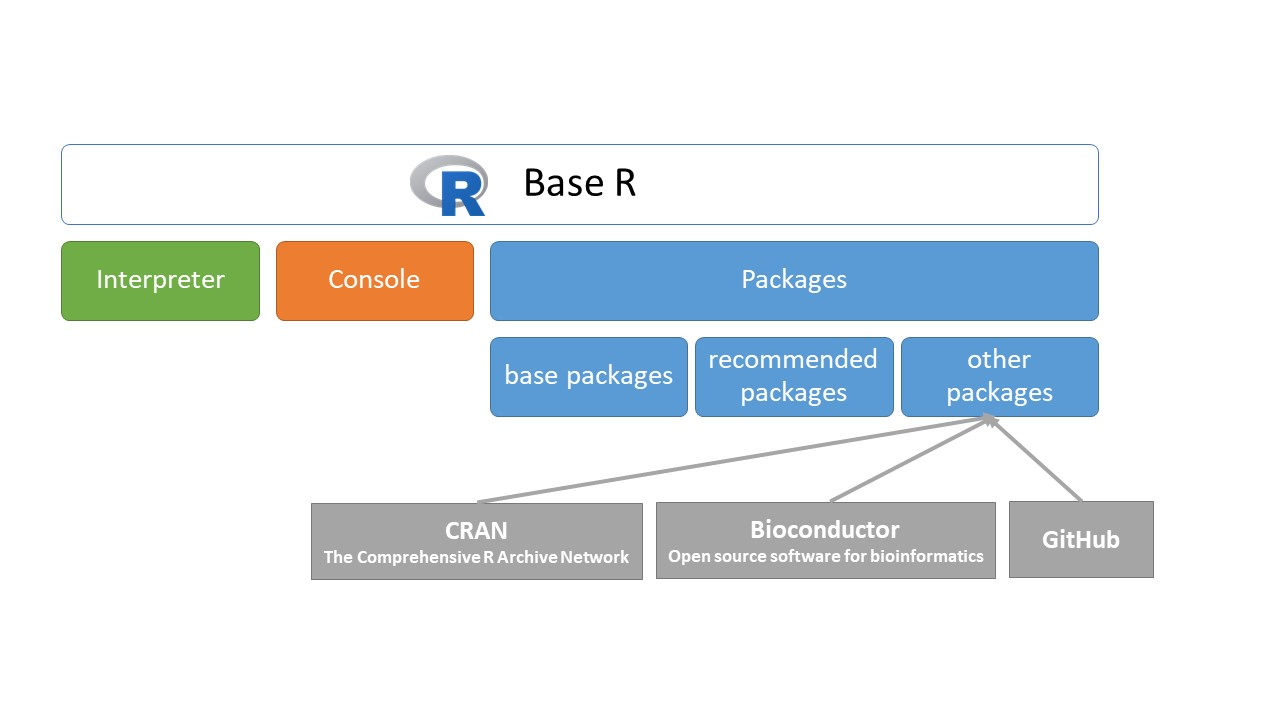
\includegraphics[width=1\linewidth]{img/baser_packages}

\begin{Shaded}
\begin{Highlighting}[]
\NormalTok{pkg }\OtherTok{\textless{}{-}} \FunctionTok{installed.packages}\NormalTok{()               }
\FunctionTok{table}\NormalTok{(pkg[,}\StringTok{"Priority"}\NormalTok{], }\AttributeTok{useNA =} \StringTok{"ifany"}\NormalTok{) }\CommentTok{\# number of installed packages}
\CommentTok{\#\textgreater{} }
\CommentTok{\#\textgreater{}        base recommended        \textless{}NA\textgreater{} }
\CommentTok{\#\textgreater{}          14          15        1684}
\end{Highlighting}
\end{Shaded}

As we can see, there are 14 base packages, 15 recommended packages in R, and I have 1684 other packages installed before.

We can print the name of base and recommended packages:

\begin{Shaded}
\begin{Highlighting}[]
\FunctionTok{rownames}\NormalTok{(pkg)[pkg[,}\StringTok{"Priority"}\NormalTok{] }\SpecialCharTok{\%in\%} \StringTok{"base"}\NormalTok{]         }\CommentTok{\# base packages}
\CommentTok{\#\textgreater{}  [1] "base"      "compiler"  "datasets"  "graphics"  "grDevices"}
\CommentTok{\#\textgreater{}  [6] "grid"      "methods"   "parallel"  "splines"   "stats"    }
\CommentTok{\#\textgreater{} [11] "stats4"    "tcltk"     "tools"     "utils"}
\FunctionTok{rownames}\NormalTok{(pkg)[pkg[,}\StringTok{"Priority"}\NormalTok{] }\SpecialCharTok{\%in\%} \StringTok{"recommended"}\NormalTok{]  }\CommentTok{\# recommended packages}
\CommentTok{\#\textgreater{}  [1] "boot"       "class"      "cluster"    "codetools" }
\CommentTok{\#\textgreater{}  [5] "foreign"    "KernSmooth" "lattice"    "MASS"      }
\CommentTok{\#\textgreater{}  [9] "Matrix"     "mgcv"       "nlme"       "nnet"      }
\CommentTok{\#\textgreater{} [13] "rpart"      "spatial"    "survival"}
\end{Highlighting}
\end{Shaded}

Only a small subset of the installed packages is actually loaded when you start an R session. This helps reduce the start-up time and avoid a behavior known as masking. The \texttt{search()} function shows you which packages are loaded on your machine.

\begin{Shaded}
\begin{Highlighting}[]
\FunctionTok{search}\NormalTok{()  }\CommentTok{\# loaded packages (with "package:" prefix)}
\CommentTok{\#\textgreater{}  [1] ".GlobalEnv"        "package:dplyr"     "package:MASS"     }
\CommentTok{\#\textgreater{}  [4] "package:stats"     "package:graphics"  "package:grDevices"}
\CommentTok{\#\textgreater{}  [7] "package:utils"     "package:datasets"  "package:methods"  }
\CommentTok{\#\textgreater{} [10] "Autoloads"         "package:base"}
\end{Highlighting}
\end{Shaded}

During starting up the R, for examle the \textbf{base}, \textbf{methods}, \textbf{datasets}, and \textbf{utils} packages are loaded automatically.

\hypertarget{load-packages}{%
\subsection{Load packages}\label{load-packages}}

To load any of installed packages, call the \texttt{library()} function. If R cannot find the specified package library, it will produce an error. For example \textbf{MASS} is a pre-installed package, part of the recommended packages. We can load it successfully.

\begin{Shaded}
\begin{Highlighting}[]
\FunctionTok{library}\NormalTok{(MASS)    }\CommentTok{\# load MASS package }
\end{Highlighting}
\end{Shaded}

We can check the loaded packages, the return value of \texttt{search()} contains the \texttt{"package:MASS"} string.

\begin{Shaded}
\begin{Highlighting}[]
\FunctionTok{search}\NormalTok{()}
\CommentTok{\#\textgreater{}  [1] ".GlobalEnv"        "package:dplyr"     "package:MASS"     }
\CommentTok{\#\textgreater{}  [4] "package:stats"     "package:graphics"  "package:grDevices"}
\CommentTok{\#\textgreater{}  [7] "package:utils"     "package:datasets"  "package:methods"  }
\CommentTok{\#\textgreater{} [10] "Autoloads"         "package:base"}
\end{Highlighting}
\end{Shaded}

But, \textbf{psych} or \textbf{DescTools} packages are part of \emph{other} packages, the \texttt{library()} function calls may cause error message (in that case we did not install them before).

\begin{Shaded}
\begin{Highlighting}[]
\FunctionTok{library}\NormalTok{(psych)      }\CommentTok{\# load psych package}
\FunctionTok{library}\NormalTok{(DescTools)  }\CommentTok{\# load DescTools package}
\end{Highlighting}
\end{Shaded}

\hypertarget{install-packages}{%
\subsection{Install packages}\label{install-packages}}

To load these packages successfully, we need to install them.

These packages are on CRAN, so we type in:

\begin{Shaded}
\begin{Highlighting}[]
\FunctionTok{install.packages}\NormalTok{(}\StringTok{"psych"}\NormalTok{)         }\CommentTok{\# installing from CRAN}
\FunctionTok{install.packages}\NormalTok{(}\StringTok{"DescTools"}\NormalTok{) }
\end{Highlighting}
\end{Shaded}

To install packages from Bioconductor, first type the following:

\begin{Shaded}
\begin{Highlighting}[]
\ControlFlowTok{if}\NormalTok{ (}\SpecialCharTok{!}\FunctionTok{requireNamespace}\NormalTok{(}\StringTok{"BiocManager"}\NormalTok{, }\AttributeTok{quietly =} \ConstantTok{TRUE}\NormalTok{))}
    \FunctionTok{install.packages}\NormalTok{(}\StringTok{"BiocManager"}\NormalTok{)}
\NormalTok{BiocManager}\SpecialCharTok{::}\FunctionTok{install}\NormalTok{()}
\end{Highlighting}
\end{Shaded}

Install specific packages, e.g., \textbf{GenomicFeatures} and \textbf{AnnotationDbi}, with

\begin{Shaded}
\begin{Highlighting}[]
\NormalTok{BiocManager}\SpecialCharTok{::}\FunctionTok{install}\NormalTok{(}\FunctionTok{c}\NormalTok{(}\StringTok{"GenomicFeatures"}\NormalTok{, }\StringTok{"AnnotationDbi"}\NormalTok{))}
\end{Highlighting}
\end{Shaded}

The third case is installing from GitHub. You can install \textbf{emo} from GitHub with:

\begin{Shaded}
\begin{Highlighting}[]
\CommentTok{\# install.packages("devtools")}
\NormalTok{devtools}\SpecialCharTok{::}\FunctionTok{install\_github}\NormalTok{(}\StringTok{"hadley/emo"}\NormalTok{)}
\end{Highlighting}
\end{Shaded}

So we can insert: 😄.

It is worth to see \href{https://github.com/trinker/pacman}{pacman: A package management tools for R} or \href{https://github.com/r-lib/remotes}{remotes} if you find an elegant way to handle packages.

Finally, we can check repository of our installed packages:

\begin{Shaded}
\begin{Highlighting}[]
\NormalTok{inst.pkg }\OtherTok{\textless{}{-}} \FunctionTok{installed.packages}\NormalTok{()[,}\DecValTok{1}\NormalTok{]  }\CommentTok{\# all installed packages}
\NormalTok{cran.pkg }\OtherTok{\textless{}{-}} \FunctionTok{available.packages}\NormalTok{(}
  \FunctionTok{contrib.url}\NormalTok{(}\AttributeTok{repos =} \StringTok{"https://cran.rstudio.com/"}\NormalTok{, }
              \AttributeTok{type =} \StringTok{"both"}\NormalTok{))         }\CommentTok{\# all CRAN packages}
\NormalTok{bioc.pkg }\OtherTok{\textless{}{-}}\NormalTok{ BiocManager}\SpecialCharTok{::}\FunctionTok{available}\NormalTok{()  }\CommentTok{\# all CRAN \& Bioconductor packages}

\FunctionTok{library}\NormalTok{(dplyr)}
\NormalTok{repos }\OtherTok{\textless{}{-}} \FunctionTok{case\_when}\NormalTok{(}
\NormalTok{  inst.pkg }\SpecialCharTok{\%in\%}\NormalTok{ cran.pkg }\SpecialCharTok{\textasciitilde{}} \StringTok{"CRAN"}\NormalTok{,}
  \SpecialCharTok{!}\NormalTok{(inst.pkg }\SpecialCharTok{\%in\%}\NormalTok{ cran.pkg) }\SpecialCharTok{\&}\NormalTok{ (inst.pkg }\SpecialCharTok{\%in\%}\NormalTok{ bioc.pkg) }\SpecialCharTok{\textasciitilde{}} \StringTok{"Bioconductor"}\NormalTok{,}
  \ConstantTok{TRUE} \SpecialCharTok{\textasciitilde{}} \StringTok{"GitHub?"} 
\NormalTok{)}
\NormalTok{df.pkg }\OtherTok{\textless{}{-}} \FunctionTok{data.frame}\NormalTok{(inst.pkg, repos)}
\FunctionTok{table}\NormalTok{(df.pkg}\SpecialCharTok{$}\NormalTok{repos)}
\CommentTok{\#\textgreater{} }
\CommentTok{\#\textgreater{} Bioconductor         CRAN      GitHub? }
\CommentTok{\#\textgreater{}           42         1646           25}
\end{Highlighting}
\end{Shaded}

\hypertarget{masking}{%
\subsection{Masking}\label{masking}}

Masking occurs when two or more ``environments'' on the search path contain one or more objects with the same name. Whenever we refer to an object by typing its name, R looks in each of the loaded environments on the search path for that object in turn, starting with the \emph{Global Environment}. If R finds an object with the name it is looking for, it stops searching. Any objects it doesn't find have been hidden, or ``masked.''

To avoid any potential masking issues, it is possible to reference an object within a package directly by using the \texttt{packageName::objectName} syntax, for example,

\begin{Shaded}
\begin{Highlighting}[]
\NormalTok{base}\SpecialCharTok{::}\NormalTok{pi}
\CommentTok{\#\textgreater{} [1] 3.141593}
\FunctionTok{str}\NormalTok{(MASS}\SpecialCharTok{::}\NormalTok{survey)}
\CommentTok{\#\textgreater{} \textquotesingle{}data.frame\textquotesingle{}:    237 obs. of  12 variables:}
\CommentTok{\#\textgreater{}  $ Sex   : Factor w/ 2 levels "Female","Male": 1 2 2 2 2 1 2 1 2 2 ...}
\CommentTok{\#\textgreater{}  $ Wr.Hnd: num  18.5 19.5 18 18.8 20 18 17.7 17 20 18.5 ...}
\CommentTok{\#\textgreater{}  $ NW.Hnd: num  18 20.5 13.3 18.9 20 17.7 17.7 17.3 19.5 18.5 ...}
\CommentTok{\#\textgreater{}  $ W.Hnd : Factor w/ 2 levels "Left","Right": 2 1 2 2 2 2 2 2 2 2 ...}
\CommentTok{\#\textgreater{}  $ Fold  : Factor w/ 3 levels "L on R","Neither",..: 3 3 1 3 2 1 1 3 3 3 ...}
\CommentTok{\#\textgreater{}  $ Pulse : int  92 104 87 NA 35 64 83 74 72 90 ...}
\CommentTok{\#\textgreater{}  $ Clap  : Factor w/ 3 levels "Left","Neither",..: 1 1 2 2 3 3 3 3 3 3 ...}
\CommentTok{\#\textgreater{}  $ Exer  : Factor w/ 3 levels "Freq","None",..: 3 2 2 2 3 3 1 1 3 3 ...}
\CommentTok{\#\textgreater{}  $ Smoke : Factor w/ 4 levels "Heavy","Never",..: 2 4 3 2 2 2 2 2 2 2 ...}
\CommentTok{\#\textgreater{}  $ Height: num  173 178 NA 160 165 ...}
\CommentTok{\#\textgreater{}  $ M.I   : Factor w/ 2 levels "Imperial","Metric": 2 1 NA 2 2 1 1 2 2 2 ...}
\CommentTok{\#\textgreater{}  $ Age   : num  18.2 17.6 16.9 20.3 23.7 ...}
\end{Highlighting}
\end{Shaded}

\hypertarget{internal-help}{%
\section{Internal help}\label{internal-help}}

The \texttt{help()} function can be used to display help on a function or indeed any R object. If you know the name of the object you require help with, you can use a function \texttt{help()} or its shorthand, \texttt{?}.

\begin{Shaded}
\begin{Highlighting}[]
\FunctionTok{help}\NormalTok{(mean)}
\NormalTok{?mean}
\end{Highlighting}
\end{Shaded}

A general search of all help files can be achieved using either the \texttt{help.search()} function or the shorthand version, \texttt{??}.

\begin{Shaded}
\begin{Highlighting}[]
\FunctionTok{help.search}\NormalTok{(}\StringTok{"test"}\NormalTok{)}
\NormalTok{??test}
\end{Highlighting}
\end{Shaded}

You can also read about any packages with \texttt{help()}function.

\begin{Shaded}
\begin{Highlighting}[]
\FunctionTok{help}\NormalTok{(}\AttributeTok{package=}\StringTok{"MASS"}\NormalTok{)}
\end{Highlighting}
\end{Shaded}

\hypertarget{getting-started-with-a-data-analysis}{%
\chapter{Getting started with a data analysis}\label{getting-started-with-a-data-analysis}}

\hypertarget{terminology}{%
\section{Terminology}\label{terminology}}

Before we begin data management tasks, we need a few vocabulary terms
would be useful to discuss. Data scientists were usually interested in
the characteristics and behaviors of humans and organizations. To
understand these things, scientists often measured and recorded
information about people or organizations.

\textbf{Dataset 1 - Marijuana legalization}

For example, a data scientist working on social science might be
interested in understanding whether age is related to votes for
marijuana legalization. To get this information, in several years,
including 2016, the \href{https://gssdataexplorer.norc.org}{GSS} survey
included a question asking the survey participants whether they support
marijuana legalization.

The GSS question was worded as follows:

\begin{itemize}
\tightlist
\item
  Do you think the use of marijuana should be legal or not?
\end{itemize}

Below the question, the different response options were listed:

\begin{itemize}
\tightlist
\item
  legal,
\item
  not legal,
\item
  don't know (\texttt{DK}),
\item
  no answer (\texttt{NA}),
\item
  not applicable (\texttt{IAP}).
\end{itemize}

The GSS Data Explorer (\url{https://gssdataexplorer.norc.org}) allows
people to create a free account and browse the data that have been
collected in the surveys. We used the Data Explorer to select the
marijuana legalization question and a question about age. The age is
important, since marijuana legalization had been primarily up to voters
so far, the success of ballot initiatives in the future will depend on
the support of people of voting age. If younger people are more
supportive, this suggests that over time, the electorate will become
more supportive as the old electorate decreases.

We saved age and vote data from the GSS and made the data file with the
file name \texttt{legal\_weed\_age\_GSS2016\_ch1.csv}. You can see the first 6 rows
from this data file:

\begin{longtable}[]{@{}ll@{}}
\caption{\label{tab:unnamed-chunk-2}Data set for marijuana legalization}\tabularnewline
\toprule
grass & age\tabularnewline
\midrule
\endfirsthead
\toprule
grass & age\tabularnewline
\midrule
\endhead
IAP & 47\tabularnewline
LEGAL & 61\tabularnewline
NOT LEGAL & 72\tabularnewline
IAP & 43\tabularnewline
LEGAL & 55\tabularnewline
LEGAL & 53\tabularnewline
\bottomrule
\end{longtable}

As you can see, each person is an \emph{observation}, and there are two \emph{variables}, voting behavior (\texttt{grass}) and \texttt{age}. In a typical \emph{dataset}, observations are the rows and variables are the columns.

\textbf{Example 2 - Student survey}

Another example a data frame contains the responses of 237 Statistics I. students at the University of Adelaide to a number of questions. It contains a lot of variables:

\begin{itemize}
\tightlist
\item
  \texttt{Sex} - The sex of the student. (Factor with levels ``Male'' and ``Female''.)
\item
  \texttt{Wr.Hnd} - span (distance from tip of thumb to tip of little finger of spread hand) of writing hand, in centimetres.
\item
  \texttt{NW.Hnd} - span of non-writing hand.
\item
  \texttt{W.Hnd} - writing hand of student. (Factor, with levels ``Left'' and ``Right''.)
\item
  \texttt{Fold} - ``Fold your arms! Which is on top'' (Factor, with levels ``R on L'', ``L on R'', ``Neither''.)
\item
  \texttt{Pulse} - pulse rate of student (beats per minute).
\item
  \texttt{Clap} - `Clap your hands! Which hand is on top?' (Factor, with levels ``Right'', ``Left'', ``Neither''.)
\item
  \texttt{Exer} - how often the student exercises. (Factor, with levels ``Freq'' (frequently), ``Some'', ``None''.)
\item
  \texttt{Smoke} - how much the student smokes. (Factor, levels ``Heavy'', ``Regul'' (regularly), ``Occas'' (occasionally), ``Never''.)
\item
  \texttt{Height} - height of the student in centimetres.
\item
  \texttt{M.I} - whether the student expressed height in imperial (feet/inches) or metric (centimetres/metres) units. (Factor, levels ``Metric'', ``Imperial''.)
\item
  \texttt{Age} - age of the student in years.
\end{itemize}

\begin{longtable}[]{@{}lrrllrlllrlr@{}}
\caption{\label{tab:unnamed-chunk-3}Student survey}\tabularnewline
\toprule
Sex & Wr.Hnd & NW.Hnd & W.Hnd & Fold & Pulse & Clap & Exer & Smoke & Height & M.I & Age\tabularnewline
\midrule
\endfirsthead
\toprule
Sex & Wr.Hnd & NW.Hnd & W.Hnd & Fold & Pulse & Clap & Exer & Smoke & Height & M.I & Age\tabularnewline
\midrule
\endhead
Female & 18.5 & 18.0 & Right & R on L & 92 & Left & Some & Never & 173.00 & Metric & 18.250\tabularnewline
Male & 19.5 & 20.5 & Left & R on L & 104 & Left & None & Regul & 177.80 & Imperial & 17.583\tabularnewline
Male & 18.0 & 13.3 & Right & L on R & 87 & Neither & None & Occas & NA & NA & 16.917\tabularnewline
Male & 18.8 & 18.9 & Right & R on L & NA & Neither & None & Never & 160.00 & Metric & 20.333\tabularnewline
Male & 20.0 & 20.0 & Right & Neither & 35 & Right & Some & Never & 165.00 & Metric & 23.667\tabularnewline
Female & 18.0 & 17.7 & Right & L on R & 64 & Right & Some & Never & 172.72 & Imperial & 21.000\tabularnewline
\bottomrule
\end{longtable}

In statistics data are organized in what we call a \emph{data matrix} or \emph{dataset}, where each row represents an observation or a case and each column represents a variable. If you ever use spreadsheets, for example an Excel spreadsheet, this representation should be familiar to you as well. There are two types of variables, numerical and categorical. Numerical, in other words, quantitative variables, take on numerical values. It is sensible to add, subtract, take averages, etc., with these values. Categorical, or qualitative variables, take on a limited number of distinct categories. These categories can be identified with numbers or labels, but it wouldn't be sensible to do arithmetic operations with these values.

Numerical variables can further be categorized as continuous or discrete. Continuous numerical variables are usually measured, such as height, and they can take on any numerical value. While we tend to round our height when we record it, it's actually measured on a continuous scale.

Discrete numerical variables are generally counted, such as the number of cars a house. These can only be whole, non-negative numbers.

Categorical variables that have ordered levels are called ordinal. Think about a survey question where you're asked how satisfied you are with the customer service you received, and the options are ``very unsatisfied'', ``unsatisfied'', ``neutral'', ``satisfied'', or ``very satisfied''. These levels have an inherent ordering, and hence the variable would be called ordinal. If the levels of a categorical variable do not have an inherent ordering to them, then the variable is
simply called nominal.

\textbf{These terms in statistics have a pair in R}. Dataset corresponds to data frame. Variable corresponds to columns of data frame. Discrete variables must be an integer or double vector in R. Continuous variables must be an integer or double vector in R, as well. Nominal or ordinal variables must be factor in R.

To sum it up, study the list below.

Terms in statistics - \textbf{terms in R} - \emph{example} :

\begin{itemize}
\item
  Data matrix, dataset - \textbf{data frame} - \emph{marijuana legalization
  dataset and survey dataset}
\item
  Variable - \textbf{columns of data frame} - \emph{each column of two dataset:
  grass, age, Sex, Wr.Hnd, etc.}

  \begin{itemize}
  \item
    numerical / quantitative

    \begin{itemize}
    \tightlist
    \item
      discrete - \textbf{integer or double vector} - \emph{Pulse}
    \item
      continuous - \textbf{integer or double vector} - \emph{age, Wr.Hnd,
      NW.Hnd, Height, Age}
    \end{itemize}
  \item
    categorical / qualitative

    \begin{itemize}
    \tightlist
    \item
      ordinal - \textbf{factor} - \emph{Exer, Smoke}
    \item
      nominal - \textbf{factor} - \emph{grass, Sex, W.Hnd, Fold, Clap, M.I}
    \end{itemize}
  \end{itemize}
\end{itemize}

\hypertarget{read-and-write-data}{%
\section{Read and write data}\label{read-and-write-data}}

R has an extensive range of functions to import many types of data files. For example, R can import data from from text files, from Microsoft Excel, from popular statistical packages, and from web sites.

\hypertarget{importing-data-from-a-delimited-text-file}{%
\subsection{Importing data from a delimited text file}\label{importing-data-from-a-delimited-text-file}}

You can import data from delimited text files using \texttt{read.table()}, a function that reads a file in table format and saves it as a data frame. Each row of the table appears as one line in the file. The syntax is

\begin{Shaded}
\begin{Highlighting}[]
\NormalTok{mydataframe }\OtherTok{\textless{}{-}} \FunctionTok{read.table}\NormalTok{(file, options)}
\end{Highlighting}
\end{Shaded}

where file is a delimited file and the options are parameters controlling how data is processed. The most common options are listed below:

\begin{itemize}
\tightlist
\item
  \texttt{header=} - A logical value indicating whether the file contains the variable names in the first line.
\item
  \texttt{sep=} - The delimiter separating data values. The default is \texttt{sep=""}, which denotes one or more spaces, tabs, new lines, or carriage returns. Use \texttt{sep=","} to read comma-delimited files, \texttt{sep="\textbackslash{}t"} to read tab-delimited files, and \texttt{sep=";"} to read semicolon-delimited files
\item
  \texttt{dec=} - The character \texttt{","} or \texttt{"."} used in the file for decimal points
\item
  \texttt{quote=} - Character(s) used to delimit strings that contain special characters. By default this is either double (\texttt{"}) or single (\texttt{\textquotesingle{}}) quotes.
\item
  \texttt{comment.char=} - A character vector of length one containing a single character or an empty string. Use "" to turn off the interpretation of comments altogether.
\item
  \texttt{fileEncoding=} - Character string for encoding name, e.g.~\texttt{"UTF-8"}, \texttt{"UTF-8-BOM"} or \texttt{"latin2"}.
\end{itemize}

Consider a text file named \texttt{legal\_weed\_age\_GSS2016\_ch1.csv} containing voters' response for marijuana legalization question and age. Each line of the file represents a student. The first line contains the variable names, separated with commas. Each subsequent line contains a voter's information, also separated with commas. The first few lines of the file are as follows:

\begin{Shaded}
\begin{Highlighting}[]
\NormalTok{grass,age}
\NormalTok{IAP,}\DecValTok{47}
\NormalTok{LEGAL,}\DecValTok{61}
\NormalTok{NOT LEGAL,}\DecValTok{72}
\NormalTok{IAP,}\DecValTok{43}
\NormalTok{LEGAL,}\DecValTok{55}
\NormalTok{LEGAL,}\DecValTok{53}
\NormalTok{IAP,}\DecValTok{50}
\NormalTok{NOT LEGAL,}\DecValTok{23}
\end{Highlighting}
\end{Shaded}

The file can be imported into a data frame using the following code:

\begin{Shaded}
\begin{Highlighting}[]
\CommentTok{\# read the GSS 2016 data }
\NormalTok{gss}\FloatTok{.2016} \OtherTok{\textless{}{-}} \FunctionTok{read.table}\NormalTok{(}\AttributeTok{file =} \StringTok{"data/legal\_weed\_age\_GSS2016\_ch1.csv"}\NormalTok{, }
                       \AttributeTok{header =}\NormalTok{ T, }\AttributeTok{sep =} \StringTok{","}\NormalTok{, }\AttributeTok{fileEncoding =} \StringTok{"UTF{-}8{-}BOM"}\NormalTok{)}
\end{Highlighting}
\end{Shaded}

The results are as follows:

\begin{Shaded}
\begin{Highlighting}[]
\FunctionTok{head}\NormalTok{(gss}\FloatTok{.2016}\NormalTok{) }\CommentTok{\# first 6 rows}
\CommentTok{\#\textgreater{}       grass age}
\CommentTok{\#\textgreater{} 1       IAP  47}
\CommentTok{\#\textgreater{} 2     LEGAL  61}
\CommentTok{\#\textgreater{} 3 NOT LEGAL  72}
\CommentTok{\#\textgreater{} 4       IAP  43}
\CommentTok{\#\textgreater{} 5     LEGAL  55}
\CommentTok{\#\textgreater{} 6     LEGAL  53}
\FunctionTok{str}\NormalTok{(gss}\FloatTok{.2016}\NormalTok{)}
\CommentTok{\#\textgreater{} \textquotesingle{}data.frame\textquotesingle{}:    2867 obs. of  2 variables:}
\CommentTok{\#\textgreater{}  $ grass: chr  "IAP" "LEGAL" "NOT LEGAL" "IAP" ...}
\CommentTok{\#\textgreater{}  $ age  : chr  "47" "61" "72" "43" ...}
\end{Highlighting}
\end{Shaded}

There are several interesting things to note about how the data is imported. By default, \texttt{read.table()} do not convert character variables to factors. You can suppress this behaviour in a number of ways. Including the option \texttt{stringsAsFactors=TRUE} turns off this behaviour for all character variables. The variable \texttt{age} is a character vector, which is not desirable. Age is a continuous variable, so it must be a numeric in R. We will discuss this issue in detail later.

\hypertarget{importing-data-from-excel}{%
\subsection{Importing data from Excel}\label{importing-data-from-excel}}

The best way to read an Excel file is to import Excel worksheets directly using the \textbf{rio} package. Be sure to download and install it before you first use it. Alternatively, export it to a comma-delimited file from Excel and import it into R using the method described earlier.

The \textbf{rio} package can be used to read, write, many file formats. The \texttt{import()} function imports a worksheet into a data frame. The simplest format is

\begin{Shaded}
\begin{Highlighting}[]
\FunctionTok{import}\NormalTok{(file)}
\end{Highlighting}
\end{Shaded}

where \texttt{file=} is the path to an Excel workbook.

Let's import the student survey: imports the first worksheet from the workbook \texttt{survey.xlsx} stored on project \texttt{data} directory and saves it as the data frame \texttt{survey}.

\begin{Shaded}
\begin{Highlighting}[]
\FunctionTok{library}\NormalTok{(rio)}
\NormalTok{survey }\OtherTok{\textless{}{-}} \FunctionTok{import}\NormalTok{(}\AttributeTok{file =} \StringTok{"data/survey.xlsx"}\NormalTok{)}
\end{Highlighting}
\end{Shaded}

The results are as follows:

\begin{Shaded}
\begin{Highlighting}[]
\FunctionTok{head}\NormalTok{(survey) }\CommentTok{\# first 6 rows}
\CommentTok{\#\textgreater{}      Sex Wr.Hnd NW.Hnd W.Hnd    Fold Pulse    Clap Exer Smoke}
\CommentTok{\#\textgreater{} 1 Female   18.5   18.0 Right  R on L    92    Left Some Never}
\CommentTok{\#\textgreater{} 2   Male   19.5   20.5  Left  R on L   104    Left None Regul}
\CommentTok{\#\textgreater{} 3   Male   18.0   13.3 Right  L on R    87 Neither None Occas}
\CommentTok{\#\textgreater{} 4   Male   18.8   18.9 Right  R on L    NA Neither None Never}
\CommentTok{\#\textgreater{} 5   Male   20.0   20.0 Right Neither    35   Right Some Never}
\CommentTok{\#\textgreater{} 6 Female   18.0   17.7 Right  L on R    64   Right Some Never}
\CommentTok{\#\textgreater{}   Height      M.I    Age}
\CommentTok{\#\textgreater{} 1 173.00   Metric 18.250}
\CommentTok{\#\textgreater{} 2 177.80 Imperial 17.583}
\CommentTok{\#\textgreater{} 3     NA     \textless{}NA\textgreater{} 16.917}
\CommentTok{\#\textgreater{} 4 160.00   Metric 20.333}
\CommentTok{\#\textgreater{} 5 165.00   Metric 23.667}
\CommentTok{\#\textgreater{} 6 172.72 Imperial 21.000}
\FunctionTok{str}\NormalTok{(survey)}
\CommentTok{\#\textgreater{} \textquotesingle{}data.frame\textquotesingle{}:    237 obs. of  12 variables:}
\CommentTok{\#\textgreater{}  $ Sex   : chr  "Female" "Male" "Male" "Male" ...}
\CommentTok{\#\textgreater{}  $ Wr.Hnd: num  18.5 19.5 18 18.8 20 18 17.7 17 20 18.5 ...}
\CommentTok{\#\textgreater{}  $ NW.Hnd: num  18 20.5 13.3 18.9 20 17.7 17.7 17.3 19.5 18.5 ...}
\CommentTok{\#\textgreater{}  $ W.Hnd : chr  "Right" "Left" "Right" "Right" ...}
\CommentTok{\#\textgreater{}  $ Fold  : chr  "R on L" "R on L" "L on R" "R on L" ...}
\CommentTok{\#\textgreater{}  $ Pulse : num  92 104 87 NA 35 64 83 74 72 90 ...}
\CommentTok{\#\textgreater{}  $ Clap  : chr  "Left" "Left" "Neither" "Neither" ...}
\CommentTok{\#\textgreater{}  $ Exer  : chr  "Some" "None" "None" "None" ...}
\CommentTok{\#\textgreater{}  $ Smoke : chr  "Never" "Regul" "Occas" "Never" ...}
\CommentTok{\#\textgreater{}  $ Height: num  173 178 NA 160 165 ...}
\CommentTok{\#\textgreater{}  $ M.I   : chr  "Metric" "Imperial" NA "Metric" ...}
\CommentTok{\#\textgreater{}  $ Age   : num  18.2 17.6 16.9 20.3 23.7 ...}
\end{Highlighting}
\end{Shaded}

As you can see, the variable \texttt{Sex}, \texttt{W.Hnd}, etc. are a character vectors, which is not desirable. They are a categorical variables, so they must be factors in R.

\hypertarget{exporting-data-from-r}{%
\subsection{Exporting data from R}\label{exporting-data-from-r}}

So far, we reviewed a wide range of methods for importing data into R. But sometimes you'll want to go the other way - exporting data from R - so that data can be archived or imported into external applications. Now, you'll learn how to output an R object to a delimited text file, an Excel spreadsheet, or a statistical application (such as SPSS, SAS, or Stata).

You can use the \texttt{write.table()} function to output an R object to a delimited text file. The format is

\begin{Shaded}
\begin{Highlighting}[]
\FunctionTok{write.table}\NormalTok{(x, outfile, }\AttributeTok{sep=}\NormalTok{delimiter, }\AttributeTok{quote=}\ConstantTok{TRUE}\NormalTok{, }\AttributeTok{na=}\StringTok{"NA"}\NormalTok{)}
\end{Highlighting}
\end{Shaded}

where \texttt{x} is the object and \texttt{outfile} is the target file. For example, the statement

\begin{Shaded}
\begin{Highlighting}[]
\FunctionTok{write.table}\NormalTok{(}\AttributeTok{x =}\NormalTok{ survey, }\AttributeTok{file =} \StringTok{"output/data/survey.txt"}\NormalTok{, }\AttributeTok{sep =} \StringTok{"}\SpecialCharTok{\textbackslash{}t}\StringTok{"}\NormalTok{, }
            \AttributeTok{dec =} \StringTok{","}\NormalTok{, }\AttributeTok{row.names =} \ConstantTok{FALSE}\NormalTok{, }\AttributeTok{quote =} \ConstantTok{FALSE}\NormalTok{)}
\end{Highlighting}
\end{Shaded}

saves the dataset \texttt{survey} to a tab-delimited file named \texttt{survey.txt} in the project \texttt{output/data} directory. Replacing \texttt{sep="\textbackslash{}t"} with \texttt{sep=";"} saves the data in a semicolon-delimited file. By default, strings are enclosed in quotes (\texttt{""}) and missing values are written as \texttt{NA}. We will not print row names (\texttt{row.names\ =\ FALSE}) and quote (\texttt{quote\ =\ FALSE}) in the output text file.

The \texttt{export()} function in the \textbf{rio} package can be used to save an R data frame to an Excel workbook. For example, the statements

\begin{Shaded}
\begin{Highlighting}[]
\FunctionTok{library}\NormalTok{(rio)}
\FunctionTok{export}\NormalTok{(}\AttributeTok{x =}\NormalTok{ gss}\FloatTok{.2016}\NormalTok{, }\AttributeTok{file =} \StringTok{"output/data/gss.xlsx"}\NormalTok{)}
\end{Highlighting}
\end{Shaded}

export the data frame \texttt{gss.2016} to a worksheet (Sheet 1 by default) in an Excel workbook named \texttt{gss.xlsx} in the project \texttt{output/data} directory. By default, the variable names in the dataset are used to create column headings in the spreadsheet, and row names are placed in the first column of the spreadsheet. If \texttt{gss.xlsx} already exists, it's overwritten.

The \texttt{export()} function in the \textbf{rio} package can be used to export a data frame to an external statistical application. For example, the code

\begin{Shaded}
\begin{Highlighting}[]
\FunctionTok{library}\NormalTok{(rio)}
\FunctionTok{export}\NormalTok{(}\AttributeTok{x =}\NormalTok{ survey, }\AttributeTok{file =} \StringTok{"output/data/survey.sav"}\NormalTok{)}
\end{Highlighting}
\end{Shaded}

exports the data frame \texttt{survey} into an SPSS data file named \texttt{survey.sav}.

Please study carefully the following codes and outputs:

\begin{Shaded}
\begin{Highlighting}[]
\CommentTok{\# Export (tab or semicolon) delimited text files with and withot encoding}
\FunctionTok{write.table}\NormalTok{(}\AttributeTok{x =}\NormalTok{ survey, }\AttributeTok{file =} \StringTok{"output/data/survey.txt"}\NormalTok{, }\AttributeTok{sep =} \StringTok{"}\SpecialCharTok{\textbackslash{}t}\StringTok{"}\NormalTok{, }
            \AttributeTok{dec =} \StringTok{","}\NormalTok{, }\AttributeTok{row.names =} \ConstantTok{FALSE}\NormalTok{, }\AttributeTok{quote =} \ConstantTok{FALSE}\NormalTok{)}
\FunctionTok{write.table}\NormalTok{(}\AttributeTok{x =}\NormalTok{ survey, }\AttributeTok{file =} \StringTok{"output/data/survey.csv"}\NormalTok{, }\AttributeTok{sep =} \StringTok{";"}\NormalTok{, }
            \AttributeTok{dec =} \StringTok{","}\NormalTok{, }\AttributeTok{row.names =} \ConstantTok{FALSE}\NormalTok{, }\AttributeTok{quote =} \ConstantTok{FALSE}\NormalTok{)}
\FunctionTok{write.table}\NormalTok{(}\AttributeTok{x =}\NormalTok{ survey, }\AttributeTok{file =} \StringTok{"output/data/survey\_utf{-}8.txt"}\NormalTok{, }\AttributeTok{sep =} \StringTok{"}\SpecialCharTok{\textbackslash{}t}\StringTok{"}\NormalTok{, }
            \AttributeTok{dec =} \StringTok{","}\NormalTok{, }\AttributeTok{row.names =} \ConstantTok{FALSE}\NormalTok{, }\AttributeTok{quote =} \ConstantTok{FALSE}\NormalTok{, }\AttributeTok{fileEncoding =} \StringTok{"UTF{-}8"}\NormalTok{)}
\FunctionTok{write.table}\NormalTok{(}\AttributeTok{x =}\NormalTok{ survey, }\AttributeTok{file =} \StringTok{"output/data/survey\_latin2.txt"}\NormalTok{, }\AttributeTok{sep =} \StringTok{"}\SpecialCharTok{\textbackslash{}t}\StringTok{"}\NormalTok{, }
            \AttributeTok{dec =} \StringTok{","}\NormalTok{, }\AttributeTok{row.names =} \ConstantTok{FALSE}\NormalTok{, }\AttributeTok{quote =} \ConstantTok{FALSE}\NormalTok{, }\AttributeTok{fileEncoding =} \StringTok{"latin2"}\NormalTok{)}
\FunctionTok{write.table}\NormalTok{(}\AttributeTok{x =}\NormalTok{ survey, }\AttributeTok{file =} \StringTok{"output/data/survey\_utf{-}8.csv"}\NormalTok{, }\AttributeTok{sep =} \StringTok{";"}\NormalTok{, }
            \AttributeTok{dec =} \StringTok{","}\NormalTok{, }\AttributeTok{row.names =} \ConstantTok{FALSE}\NormalTok{, }\AttributeTok{quote =} \ConstantTok{FALSE}\NormalTok{, }\AttributeTok{fileEncoding =} \StringTok{"UTF{-}8"}\NormalTok{)}
\FunctionTok{write.table}\NormalTok{(}\AttributeTok{x =}\NormalTok{ survey, }\AttributeTok{file =} \StringTok{"output/data/survey\_latin2.csv"}\NormalTok{, }\AttributeTok{sep =} \StringTok{";"}\NormalTok{, }
            \AttributeTok{dec =} \StringTok{","}\NormalTok{, }\AttributeTok{row.names =} \ConstantTok{FALSE}\NormalTok{, }\AttributeTok{quote =} \ConstantTok{FALSE}\NormalTok{, }\AttributeTok{fileEncoding =} \StringTok{"latin2"}\NormalTok{)}

\CommentTok{\# Export Excel and SPSS files}
\FunctionTok{library}\NormalTok{(rio)}
\FunctionTok{export}\NormalTok{(}\AttributeTok{x =}\NormalTok{ survey, }\AttributeTok{file =} \StringTok{"output/data/survey.xlsx"}\NormalTok{)}
\FunctionTok{export}\NormalTok{(}\AttributeTok{x =}\NormalTok{ survey, }\AttributeTok{file =} \StringTok{"output/data/survey.sav"}\NormalTok{)}
\FunctionTok{export}\NormalTok{(}\AttributeTok{x =}\NormalTok{ gss}\FloatTok{.2016}\NormalTok{, }\AttributeTok{file =} \StringTok{"output/data/gss.xlsx"}\NormalTok{)}
\FunctionTok{export}\NormalTok{(}\AttributeTok{x =}\NormalTok{ gss}\FloatTok{.2016}\NormalTok{, }\AttributeTok{file =} \StringTok{"output/data/gss.sav"}\NormalTok{)}
\end{Highlighting}
\end{Shaded}

\hypertarget{data-manipulation}{%
\section{Data manipulation}\label{data-manipulation}}

In the previous chapter, we covered a variety of methods for importing data into R. Unfortunately, getting your data in the rectangular arrangement of a matrix or data frame is only the first step in preparing it for analysis. In this early stage we try to get as much information as we can.

\hypertarget{get-information}{%
\subsection{Get information}\label{get-information}}

When working with (large) data frames, you must first develop a clear understanding of the structure and main elements of the data set. Therefore, it can often be useful to show only a small part of the entire data set. To do this in R, you can use the functions \texttt{head()} or \texttt{tail()}. The \texttt{head()} function shows the first part of the data frame. The \texttt{tail()} function shows the last part. Both functions print a top line called the \emph{header} which contains the names of the different variables in the data set.

\begin{Shaded}
\begin{Highlighting}[]
\FunctionTok{head}\NormalTok{(gss}\FloatTok{.2016}\NormalTok{)}
\CommentTok{\#\textgreater{}       grass age}
\CommentTok{\#\textgreater{} 1       IAP  47}
\CommentTok{\#\textgreater{} 2     LEGAL  61}
\CommentTok{\#\textgreater{} 3 NOT LEGAL  72}
\CommentTok{\#\textgreater{} 4       IAP  43}
\CommentTok{\#\textgreater{} 5     LEGAL  55}
\CommentTok{\#\textgreater{} 6     LEGAL  53}
\FunctionTok{tail}\NormalTok{(gss}\FloatTok{.2016}\NormalTok{, }\AttributeTok{n =} \DecValTok{3}\NormalTok{)}
\CommentTok{\#\textgreater{}          grass age}
\CommentTok{\#\textgreater{} 2865     LEGAL  87}
\CommentTok{\#\textgreater{} 2866       IAP  55}
\CommentTok{\#\textgreater{} 2867 NOT LEGAL  72}
\end{Highlighting}
\end{Shaded}

Another method to get a rapid overview of the data is the \texttt{str()} function. The \texttt{str()} function shows the structure of the data set.

\begin{Shaded}
\begin{Highlighting}[]
\FunctionTok{str}\NormalTok{(gss}\FloatTok{.2016}\NormalTok{)}
\CommentTok{\#\textgreater{} \textquotesingle{}data.frame\textquotesingle{}:    2867 obs. of  2 variables:}
\CommentTok{\#\textgreater{}  $ grass: chr  "IAP" "LEGAL" "NOT LEGAL" "IAP" ...}
\CommentTok{\#\textgreater{}  $ age  : chr  "47" "61" "72" "43" ...}
\end{Highlighting}
\end{Shaded}

For a data frame it gives the following information:

\begin{itemize}
\tightlist
\item
  The total number of observations (e.g.~2867 voters)
\item
  The total number of variables (e.g.~2 variables)
\item
  A full list of the variables names (\texttt{grass}, \texttt{age})
\item
  The data type of each variable (\texttt{chr} )
\item
  The first observations
\end{itemize}

When you receive a new data frame, applying the \texttt{str()} function is often the first step. It is a great way to get more insight into the data set before deeper analysis.

Please study carefully the following codes and outputs:

\begin{Shaded}
\begin{Highlighting}[]
\FunctionTok{str}\NormalTok{(gss}\FloatTok{.2016}\NormalTok{)        }\CommentTok{\# Structure of an Arbitrary R Object}
\CommentTok{\#\textgreater{} \textquotesingle{}data.frame\textquotesingle{}:    2867 obs. of  2 variables:}
\CommentTok{\#\textgreater{}  $ grass: chr  "IAP" "LEGAL" "NOT LEGAL" "IAP" ...}
\CommentTok{\#\textgreater{}  $ age  : chr  "47" "61" "72" "43" ...}
\FunctionTok{head}\NormalTok{(gss}\FloatTok{.2016}\NormalTok{)       }\CommentTok{\# Return the First Parts of an Object}
\CommentTok{\#\textgreater{}       grass age}
\CommentTok{\#\textgreater{} 1       IAP  47}
\CommentTok{\#\textgreater{} 2     LEGAL  61}
\CommentTok{\#\textgreater{} 3 NOT LEGAL  72}
\CommentTok{\#\textgreater{} 4       IAP  43}
\CommentTok{\#\textgreater{} 5     LEGAL  55}
\CommentTok{\#\textgreater{} 6     LEGAL  53}
\FunctionTok{dim}\NormalTok{(gss}\FloatTok{.2016}\NormalTok{)        }\CommentTok{\# Dimensions of an Object}
\CommentTok{\#\textgreater{} [1] 2867    2}
\FunctionTok{ncol}\NormalTok{(gss}\FloatTok{.2016}\NormalTok{)       }\CommentTok{\# The Number of Rows of a data frame}
\CommentTok{\#\textgreater{} [1] 2}
\FunctionTok{nrow}\NormalTok{(gss}\FloatTok{.2016}\NormalTok{)       }\CommentTok{\# The Number of Columns of a data frame}
\CommentTok{\#\textgreater{} [1] 2867}
\FunctionTok{names}\NormalTok{(gss}\FloatTok{.2016}\NormalTok{)      }\CommentTok{\# The Column Names of an Object}
\CommentTok{\#\textgreater{} [1] "grass" "age"}
\FunctionTok{typeof}\NormalTok{(gss}\FloatTok{.2016}\NormalTok{)     }\CommentTok{\# Type of an Object}
\CommentTok{\#\textgreater{} [1] "list"}
\FunctionTok{class}\NormalTok{(gss}\FloatTok{.2016}\NormalTok{)      }\CommentTok{\# Class of an Object}
\CommentTok{\#\textgreater{} [1] "data.frame"}
\FunctionTok{str}\NormalTok{(survey)}
\CommentTok{\#\textgreater{} \textquotesingle{}data.frame\textquotesingle{}:    237 obs. of  12 variables:}
\CommentTok{\#\textgreater{}  $ Sex   : chr  "Female" "Male" "Male" "Male" ...}
\CommentTok{\#\textgreater{}  $ Wr.Hnd: num  18.5 19.5 18 18.8 20 18 17.7 17 20 18.5 ...}
\CommentTok{\#\textgreater{}  $ NW.Hnd: num  18 20.5 13.3 18.9 20 17.7 17.7 17.3 19.5 18.5 ...}
\CommentTok{\#\textgreater{}  $ W.Hnd : chr  "Right" "Left" "Right" "Right" ...}
\CommentTok{\#\textgreater{}  $ Fold  : chr  "R on L" "R on L" "L on R" "R on L" ...}
\CommentTok{\#\textgreater{}  $ Pulse : num  92 104 87 NA 35 64 83 74 72 90 ...}
\CommentTok{\#\textgreater{}  $ Clap  : chr  "Left" "Left" "Neither" "Neither" ...}
\CommentTok{\#\textgreater{}  $ Exer  : chr  "Some" "None" "None" "None" ...}
\CommentTok{\#\textgreater{}  $ Smoke : chr  "Never" "Regul" "Occas" "Never" ...}
\CommentTok{\#\textgreater{}  $ Height: num  173 178 NA 160 165 ...}
\CommentTok{\#\textgreater{}  $ M.I   : chr  "Metric" "Imperial" NA "Metric" ...}
\CommentTok{\#\textgreater{}  $ Age   : num  18.2 17.6 16.9 20.3 23.7 ...}
\FunctionTok{head}\NormalTok{(survey)}
\CommentTok{\#\textgreater{}      Sex Wr.Hnd NW.Hnd W.Hnd    Fold Pulse    Clap Exer Smoke}
\CommentTok{\#\textgreater{} 1 Female   18.5   18.0 Right  R on L    92    Left Some Never}
\CommentTok{\#\textgreater{} 2   Male   19.5   20.5  Left  R on L   104    Left None Regul}
\CommentTok{\#\textgreater{} 3   Male   18.0   13.3 Right  L on R    87 Neither None Occas}
\CommentTok{\#\textgreater{} 4   Male   18.8   18.9 Right  R on L    NA Neither None Never}
\CommentTok{\#\textgreater{} 5   Male   20.0   20.0 Right Neither    35   Right Some Never}
\CommentTok{\#\textgreater{} 6 Female   18.0   17.7 Right  L on R    64   Right Some Never}
\CommentTok{\#\textgreater{}   Height      M.I    Age}
\CommentTok{\#\textgreater{} 1 173.00   Metric 18.250}
\CommentTok{\#\textgreater{} 2 177.80 Imperial 17.583}
\CommentTok{\#\textgreater{} 3     NA     \textless{}NA\textgreater{} 16.917}
\CommentTok{\#\textgreater{} 4 160.00   Metric 20.333}
\CommentTok{\#\textgreater{} 5 165.00   Metric 23.667}
\CommentTok{\#\textgreater{} 6 172.72 Imperial 21.000}
\FunctionTok{dim}\NormalTok{(survey)}
\CommentTok{\#\textgreater{} [1] 237  12}
\FunctionTok{ncol}\NormalTok{(survey)}
\CommentTok{\#\textgreater{} [1] 12}
\FunctionTok{nrow}\NormalTok{(survey)}
\CommentTok{\#\textgreater{} [1] 237}
\FunctionTok{names}\NormalTok{(survey)}
\CommentTok{\#\textgreater{}  [1] "Sex"    "Wr.Hnd" "NW.Hnd" "W.Hnd"  "Fold"   "Pulse" }
\CommentTok{\#\textgreater{}  [7] "Clap"   "Exer"   "Smoke"  "Height" "M.I"    "Age"}
\FunctionTok{typeof}\NormalTok{(survey)}
\CommentTok{\#\textgreater{} [1] "list"}
\FunctionTok{class}\NormalTok{(survey)}
\CommentTok{\#\textgreater{} [1] "data.frame"}
\end{Highlighting}
\end{Shaded}

\hypertarget{data-type-conversions}{%
\subsection{Data type conversions}\label{data-type-conversions}}

As you have known, in R, you use numeric vectors to represent quantitative variables, and you use factors to represent categorical variables. In the data frame \texttt{gss.2016}, the variable \texttt{grass} is character vector, but it should be a factor. R provides a set of functions to identify an object's data type and convert it to a different data type. You can use the function \texttt{factor()} to convert from character or numeric to factor.

\begin{Shaded}
\begin{Highlighting}[]
\FunctionTok{str}\NormalTok{(gss}\FloatTok{.2016}\NormalTok{)                             }\CommentTok{\# grass is character}
\CommentTok{\#\textgreater{} \textquotesingle{}data.frame\textquotesingle{}:    2867 obs. of  2 variables:}
\CommentTok{\#\textgreater{}  $ grass: chr  "IAP" "LEGAL" "NOT LEGAL" "IAP" ...}
\CommentTok{\#\textgreater{}  $ age  : chr  "47" "61" "72" "43" ...}
\NormalTok{gss}\FloatTok{.2016}\SpecialCharTok{$}\NormalTok{grass }\OtherTok{\textless{}{-}} \FunctionTok{factor}\NormalTok{(gss}\FloatTok{.2016}\SpecialCharTok{$}\NormalTok{grass)  }\CommentTok{\# convert}
\FunctionTok{str}\NormalTok{(gss}\FloatTok{.2016}\NormalTok{)                             }\CommentTok{\# grass is factor}
\CommentTok{\#\textgreater{} \textquotesingle{}data.frame\textquotesingle{}:    2867 obs. of  2 variables:}
\CommentTok{\#\textgreater{}  $ grass: Factor w/ 4 levels "DK","IAP","LEGAL",..: 2 3 4 2 3 3 2 4 2 4 ...}
\CommentTok{\#\textgreater{}  $ age  : chr  "47" "61" "72" "43" ...}
\end{Highlighting}
\end{Shaded}

The continuous variable \texttt{age} is also character, but it should be a numeric. What is the problem with age variable? Use the \texttt{unique()} and \texttt{table()} functions.

\begin{Shaded}
\begin{Highlighting}[]
\FunctionTok{unique}\NormalTok{(gss}\FloatTok{.2016}\SpecialCharTok{$}\NormalTok{age)}
\CommentTok{\#\textgreater{}  [1] "47"          "61"          "72"          "43"         }
\CommentTok{\#\textgreater{}  [5] "55"          "53"          "50"          "23"         }
\CommentTok{\#\textgreater{}  [9] "45"          "71"          "33"          "86"         }
\CommentTok{\#\textgreater{} [13] "32"          "60"          "76"          "56"         }
\CommentTok{\#\textgreater{} [17] "62"          "31"          "58"          "37"         }
\CommentTok{\#\textgreater{} [21] "25"          "22"          "74"          "75"         }
\CommentTok{\#\textgreater{} [25] "68"          "46"          "35"          "59"         }
\CommentTok{\#\textgreater{} [29] "79"          "40"          "44"          "36"         }
\CommentTok{\#\textgreater{} [33] "70"          "28"          "20"          "41"         }
\CommentTok{\#\textgreater{} [37] "42"          "57"          "26"          "51"         }
\CommentTok{\#\textgreater{} [41] "39"          "27"          "30"          "29"         }
\CommentTok{\#\textgreater{} [45] "80"          "49"          "78"          "52"         }
\CommentTok{\#\textgreater{} [49] "66"          "89 OR OLDER" "54"          "48"         }
\CommentTok{\#\textgreater{} [53] "81"          "69"          "21"          "64"         }
\CommentTok{\#\textgreater{} [57] "38"          "65"          "67"          "84"         }
\CommentTok{\#\textgreater{} [61] "34"          "77"          "19"          NA           }
\CommentTok{\#\textgreater{} [65] "83"          "73"          "63"          "24"         }
\CommentTok{\#\textgreater{} [69] "82"          "85"          "87"          "18"         }
\CommentTok{\#\textgreater{} [73] "88"}
\FunctionTok{table}\NormalTok{(gss}\FloatTok{.2016}\SpecialCharTok{$}\NormalTok{age, }\AttributeTok{useNA =} \StringTok{"ifany"}\NormalTok{)}
\CommentTok{\#\textgreater{} }
\CommentTok{\#\textgreater{}          18          19          20          21          22 }
\CommentTok{\#\textgreater{}           7          33          26          33          44 }
\CommentTok{\#\textgreater{}          23          24          25          26          27 }
\CommentTok{\#\textgreater{}          49          35          56          42          58 }
\CommentTok{\#\textgreater{}          28          29          30          31          32 }
\CommentTok{\#\textgreater{}          42          56          54          57          42 }
\CommentTok{\#\textgreater{}          33          34          35          36          37 }
\CommentTok{\#\textgreater{}          54          49          56          52          58 }
\CommentTok{\#\textgreater{}          38          39          40          41          42 }
\CommentTok{\#\textgreater{}          44          42          46          36          50 }
\CommentTok{\#\textgreater{}          43          44          45          46          47 }
\CommentTok{\#\textgreater{}          45          52          27          45          55 }
\CommentTok{\#\textgreater{}          48          49          50          51          52 }
\CommentTok{\#\textgreater{}          46          41          48          49          65 }
\CommentTok{\#\textgreater{}          53          54          55          56          57 }
\CommentTok{\#\textgreater{}          60          53          48          48          70 }
\CommentTok{\#\textgreater{}          58          59          60          61          62 }
\CommentTok{\#\textgreater{}          67          58          53          56          56 }
\CommentTok{\#\textgreater{}          63          64          65          66          67 }
\CommentTok{\#\textgreater{}          43          34          44          47          49 }
\CommentTok{\#\textgreater{}          68          69          70          71          72 }
\CommentTok{\#\textgreater{}          43          42          32          27          26 }
\CommentTok{\#\textgreater{}          73          74          75          76          77 }
\CommentTok{\#\textgreater{}          22          24          19          25          23 }
\CommentTok{\#\textgreater{}          78          79          80          81          82 }
\CommentTok{\#\textgreater{}          26          21          25          21          11 }
\CommentTok{\#\textgreater{}          83          84          85          86          87 }
\CommentTok{\#\textgreater{}          22          11          11          12           9 }
\CommentTok{\#\textgreater{}          88 89 OR OLDER        \textless{}NA\textgreater{} }
\CommentTok{\#\textgreater{}           3          22          10}
\end{Highlighting}
\end{Shaded}

\texttt{unique(x)} returns an object of the same type of \texttt{x}, but with only one copy of each duplicated element. \texttt{table(x)} returns the same, plus the number of times a particular value of \texttt{x} occurs.

Age appears to be measured in years up to age 88, and then \texttt{"89\ OR\ OLDER"} represents people who are 89 years old or older. Since \texttt{"89\ OR\ OLDER"} can not be a number, trying to force the age variable with \texttt{"89\ OR\ OLDER"} in it into a numeric variable would result in an error. Before converting \texttt{age} into a numeric variable, you should first recode anyone who has a value of \texttt{"89\ OR\ OLDER"} to instead have a value 89.

\begin{Shaded}
\begin{Highlighting}[]
\NormalTok{gss}\FloatTok{.2016}\SpecialCharTok{$}\NormalTok{age[gss}\FloatTok{.2016}\SpecialCharTok{$}\NormalTok{age }\SpecialCharTok{\%in\%} \StringTok{"89 OR OLDER"}\NormalTok{] }\OtherTok{\textless{}{-}} \StringTok{"89"}  \CommentTok{\# recoding}
\NormalTok{gss}\FloatTok{.2016}\SpecialCharTok{$}\NormalTok{age }\OtherTok{\textless{}{-}} \FunctionTok{as.numeric}\NormalTok{(gss}\FloatTok{.2016}\SpecialCharTok{$}\NormalTok{age)               }\CommentTok{\# data type conversion}
\FunctionTok{str}\NormalTok{(gss}\FloatTok{.2016}\NormalTok{) }
\CommentTok{\#\textgreater{} \textquotesingle{}data.frame\textquotesingle{}:    2867 obs. of  2 variables:}
\CommentTok{\#\textgreater{}  $ grass: Factor w/ 4 levels "DK","IAP","LEGAL",..: 2 3 4 2 3 3 2 4 2 4 ...}
\CommentTok{\#\textgreater{}  $ age  : num  47 61 72 43 55 53 50 23 45 71 ...}
\end{Highlighting}
\end{Shaded}

By now, the data frame \texttt{gss.2016} is in the desired structure.

What about the data frame \texttt{survey}? As we mentioned, there are a few variables, namely \texttt{Sex}, \texttt{W.Hnd}, \texttt{Fold}, \texttt{Clap}, \texttt{Exer},\texttt{Smoke}, and\texttt{M.I}, that are categorical, so you need to convert to factor. We can use the \texttt{factor()} function:

\begin{Shaded}
\begin{Highlighting}[]
\NormalTok{survey}\SpecialCharTok{$}\NormalTok{Sex }\OtherTok{\textless{}{-}} \FunctionTok{factor}\NormalTok{(survey}\SpecialCharTok{$}\NormalTok{Sex)}
\NormalTok{survey}\SpecialCharTok{$}\NormalTok{W.Hnd }\OtherTok{\textless{}{-}} \FunctionTok{factor}\NormalTok{(survey}\SpecialCharTok{$}\NormalTok{W.Hnd)}
\NormalTok{survey}\SpecialCharTok{$}\NormalTok{Fold }\OtherTok{\textless{}{-}} \FunctionTok{factor}\NormalTok{(survey}\SpecialCharTok{$}\NormalTok{Fold)}
\NormalTok{survey}\SpecialCharTok{$}\NormalTok{Clap }\OtherTok{\textless{}{-}} \FunctionTok{factor}\NormalTok{(survey}\SpecialCharTok{$}\NormalTok{Clap)}
\NormalTok{survey}\SpecialCharTok{$}\NormalTok{Exer }\OtherTok{\textless{}{-}} \FunctionTok{factor}\NormalTok{(survey}\SpecialCharTok{$}\NormalTok{Exer)}
\NormalTok{survey}\SpecialCharTok{$}\NormalTok{Smoke }\OtherTok{\textless{}{-}} \FunctionTok{factor}\NormalTok{(survey}\SpecialCharTok{$}\NormalTok{Smoke)}
\NormalTok{survey}\SpecialCharTok{$}\NormalTok{M.I }\OtherTok{\textless{}{-}} \FunctionTok{factor}\NormalTok{(survey}\SpecialCharTok{$}\NormalTok{M.I)}
\FunctionTok{str}\NormalTok{(survey)}
\CommentTok{\#\textgreater{} \textquotesingle{}data.frame\textquotesingle{}:    237 obs. of  12 variables:}
\CommentTok{\#\textgreater{}  $ Sex   : Factor w/ 2 levels "Female","Male": 1 2 2 2 2 1 2 1 2 2 ...}
\CommentTok{\#\textgreater{}  $ Wr.Hnd: num  18.5 19.5 18 18.8 20 18 17.7 17 20 18.5 ...}
\CommentTok{\#\textgreater{}  $ NW.Hnd: num  18 20.5 13.3 18.9 20 17.7 17.7 17.3 19.5 18.5 ...}
\CommentTok{\#\textgreater{}  $ W.Hnd : Factor w/ 2 levels "Left","Right": 2 1 2 2 2 2 2 2 2 2 ...}
\CommentTok{\#\textgreater{}  $ Fold  : Factor w/ 3 levels "L on R","Neither",..: 3 3 1 3 2 1 1 3 3 3 ...}
\CommentTok{\#\textgreater{}  $ Pulse : num  92 104 87 NA 35 64 83 74 72 90 ...}
\CommentTok{\#\textgreater{}  $ Clap  : Factor w/ 3 levels "Left","Neither",..: 1 1 2 2 3 3 3 3 3 3 ...}
\CommentTok{\#\textgreater{}  $ Exer  : Factor w/ 3 levels "Freq","None",..: 3 2 2 2 3 3 1 1 3 3 ...}
\CommentTok{\#\textgreater{}  $ Smoke : Factor w/ 4 levels "Heavy","Never",..: 2 4 3 2 2 2 2 2 2 2 ...}
\CommentTok{\#\textgreater{}  $ Height: num  173 178 NA 160 165 ...}
\CommentTok{\#\textgreater{}  $ M.I   : Factor w/ 2 levels "Imperial","Metric": 2 1 NA 2 2 1 1 2 2 2 ...}
\CommentTok{\#\textgreater{}  $ Age   : num  18.2 17.6 16.9 20.3 23.7 ...}
\end{Highlighting}
\end{Shaded}

Our dataset \texttt{survey} contains only numeric and factor variables. But two variables (\texttt{Exer} an\texttt{Smoke}) are ordinal categorical variable, so you need to check the levels.

Sometimes it's useful to know the number of levels of a factor. The convenience function \texttt{nlevels()} extracts the number of levels from a factor:

\begin{Shaded}
\begin{Highlighting}[]
\FunctionTok{nlevels}\NormalTok{(survey}\SpecialCharTok{$}\NormalTok{Exer)}
\CommentTok{\#\textgreater{} [1] 3}
\end{Highlighting}
\end{Shaded}

To look at the levels of a factor, you use the \texttt{levels()} function. For example,
to extract the factor levels of \texttt{Exer}, use the following:

\begin{Shaded}
\begin{Highlighting}[]
\FunctionTok{levels}\NormalTok{(survey}\SpecialCharTok{$}\NormalTok{Exer)}
\CommentTok{\#\textgreater{} [1] "Freq" "None" "Some"}
\end{Highlighting}
\end{Shaded}

As you can see, each student has a status of exercise (None, Some, Freq), how often the student exercises. Notice, in the output above the levels are ordered alphabetically. However, we need to sort in the order None, Some, Freq:

\begin{Shaded}
\begin{Highlighting}[]
\NormalTok{survey}\SpecialCharTok{$}\NormalTok{Exer }\OtherTok{\textless{}{-}} \FunctionTok{factor}\NormalTok{(survey}\SpecialCharTok{$}\NormalTok{Exer, }\AttributeTok{levels=}\FunctionTok{c}\NormalTok{(}\StringTok{"None"}\NormalTok{, }\StringTok{"Some"}\NormalTok{, }\StringTok{"Freq"}\NormalTok{))}
\FunctionTok{levels}\NormalTok{(survey}\SpecialCharTok{$}\NormalTok{Exer)}
\CommentTok{\#\textgreater{} [1] "None" "Some" "Freq"}
\end{Highlighting}
\end{Shaded}

In R, there is a really big practical advantage to order factor's level. A great
many R functions recognize and treat ordered factors differently by printing results in the order that you expect. For example,

\begin{Shaded}
\begin{Highlighting}[]
\FunctionTok{table}\NormalTok{(survey}\SpecialCharTok{$}\NormalTok{Exer, }\AttributeTok{useNA =} \StringTok{"ifany"}\NormalTok{)}
\CommentTok{\#\textgreater{} }
\CommentTok{\#\textgreater{} None Some Freq }
\CommentTok{\#\textgreater{}   24   98  115}
\end{Highlighting}
\end{Shaded}

We need to order the levels in \texttt{Smoke} variable.

\begin{Shaded}
\begin{Highlighting}[]
\FunctionTok{levels}\NormalTok{(survey}\SpecialCharTok{$}\NormalTok{Smoke)}
\CommentTok{\#\textgreater{} [1] "Heavy" "Never" "Occas" "Regul"}
\FunctionTok{table}\NormalTok{(survey}\SpecialCharTok{$}\NormalTok{Smoke, }\AttributeTok{useNA =} \StringTok{"ifany"}\NormalTok{)}
\CommentTok{\#\textgreater{} }
\CommentTok{\#\textgreater{} Heavy Never Occas Regul  \textless{}NA\textgreater{} }
\CommentTok{\#\textgreater{}    11   189    19    17     1}
\NormalTok{survey}\SpecialCharTok{$}\NormalTok{Smoke }\OtherTok{\textless{}{-}} \FunctionTok{factor}\NormalTok{(survey}\SpecialCharTok{$}\NormalTok{Smoke, }\AttributeTok{levels=}\FunctionTok{c}\NormalTok{(}\StringTok{"Never"}\NormalTok{, }\StringTok{"Occas"}\NormalTok{, }\StringTok{"Regul"}\NormalTok{,}\StringTok{"Heavy"}\NormalTok{))}
\FunctionTok{levels}\NormalTok{(survey}\SpecialCharTok{$}\NormalTok{Smoke)}
\CommentTok{\#\textgreater{} [1] "Never" "Occas" "Regul" "Heavy"}
\FunctionTok{table}\NormalTok{(survey}\SpecialCharTok{$}\NormalTok{Smoke, }\AttributeTok{useNA =} \StringTok{"ifany"}\NormalTok{)}
\CommentTok{\#\textgreater{} }
\CommentTok{\#\textgreater{} Never Occas Regul Heavy  \textless{}NA\textgreater{} }
\CommentTok{\#\textgreater{}   189    19    17    11     1}
\end{Highlighting}
\end{Shaded}

\hypertarget{transformation}{%
\subsection{Transformation}\label{transformation}}

\hypertarget{identifying-and-treating-missing-values}{%
\subsection{Identifying and treating missing values}\label{identifying-and-treating-missing-values}}

In addition to making sure the variables used are an appropriate type, it was also important to make sure that missing values were treated appropriately by R. In R, missing values are recorded as \texttt{NA}, which stands for not available. Researchers code missing values in many different ways when collecting and storing data. Some of the more common ways to denote missing values are the following:

\begin{itemize}
\tightlist
\item
  blank
\item
  777, -777, 888, -888, 999, -999, or something similar
\item
  a single period
\item
  -1
\item
  NULL.
\end{itemize}

Other responses, such as ``Don't know'' or ``Inapplicable,'' may sometimes be treated as missing or as response categories depending on what is most appropriate given the characteristics of the data and the analysis goals.

In the summary of the \texttt{gss.2016} data,

\begin{Shaded}
\begin{Highlighting}[]
\FunctionTok{summary}\NormalTok{(gss}\FloatTok{.2016}\NormalTok{)}
\CommentTok{\#\textgreater{}        grass           age       }
\CommentTok{\#\textgreater{}  DK       : 110   Min.   :18.00  }
\CommentTok{\#\textgreater{}  IAP      : 911   1st Qu.:34.00  }
\CommentTok{\#\textgreater{}  LEGAL    :1126   Median :49.00  }
\CommentTok{\#\textgreater{}  NOT LEGAL: 717   Mean   :49.16  }
\CommentTok{\#\textgreater{}  NA\textquotesingle{}s     :   3   3rd Qu.:62.00  }
\CommentTok{\#\textgreater{}                   Max.   :89.00  }
\CommentTok{\#\textgreater{}                   NA\textquotesingle{}s   :10}
\end{Highlighting}
\end{Shaded}

the \texttt{grass} variable has five possible values: \texttt{DK} (don't know), \texttt{IAP} (inapplicable), \texttt{LEGAL}, \texttt{NOT\ LEGAL}, and \texttt{NA} (not available). The \texttt{DK}, \texttt{IAP}, and \texttt{NA} could all be considered missing values. However, R treats only \texttt{NA} as missing. Before conducting any analyses, the \texttt{DK} and \texttt{IAP} values could be converted to \texttt{NA} to be treated as missing in any analyses. That is, the \texttt{grass} variable could be recoded so that these values are all \texttt{NA}. Note that \texttt{NA} is a reserved ``word'' in R. In order to use \texttt{NA}, both letters must be uppercase (\texttt{Na} or \texttt{na} does not work), and there can be no quotation marks (R will treat \texttt{"NA"} as a character rather than a true missing value). There are many ways to recode variables in R. For example,

\begin{Shaded}
\begin{Highlighting}[]
\FunctionTok{table}\NormalTok{(gss}\FloatTok{.2016}\SpecialCharTok{$}\NormalTok{grass, }\AttributeTok{useNA =} \StringTok{"ifany"}\NormalTok{)   }\CommentTok{\# before recoding}
\CommentTok{\#\textgreater{} }
\CommentTok{\#\textgreater{}        DK       IAP     LEGAL NOT LEGAL      \textless{}NA\textgreater{} }
\CommentTok{\#\textgreater{}       110       911      1126       717         3}
\FunctionTok{library}\NormalTok{(car)}
\NormalTok{gss}\FloatTok{.2016}\SpecialCharTok{$}\NormalTok{grass }\OtherTok{\textless{}{-}}\NormalTok{ car}\SpecialCharTok{::}\FunctionTok{recode}\NormalTok{(}\AttributeTok{var =}\NormalTok{ gss}\FloatTok{.2016}\SpecialCharTok{$}\NormalTok{grass, }\AttributeTok{recodes =} \StringTok{\textquotesingle{}c("DK", "IAP")=NA\textquotesingle{}}\NormalTok{)}
\FunctionTok{table}\NormalTok{(gss}\FloatTok{.2016}\SpecialCharTok{$}\NormalTok{grass, }\AttributeTok{useNA =} \StringTok{"ifany"}\NormalTok{)   }\CommentTok{\# after recoding}
\CommentTok{\#\textgreater{} }
\CommentTok{\#\textgreater{}     LEGAL NOT LEGAL      \textless{}NA\textgreater{} }
\CommentTok{\#\textgreater{}      1126       717      1024}
\end{Highlighting}
\end{Shaded}

\hypertarget{numeric-to-factor}{%
\subsection{Numeric to factor}\label{numeric-to-factor}}

In addition to solving the \texttt{age} and \texttt{grass} recoding, the final plan to create the age categories shown below. The \texttt{age} variable currently holds the age in years rather than age categories. The age can be in four categories:

\begin{itemize}
\tightlist
\item
  18-29
\item
  30-59
\item
  60-74
\item
  75+
\end{itemize}

The function \texttt{cut()} can be used to divide a continuous variable into categories by cutting it into pieces and adding a label to each piece.

\begin{Shaded}
\begin{Highlighting}[]
\NormalTok{gss}\FloatTok{.2016}\SpecialCharTok{$}\NormalTok{age.f }\OtherTok{\textless{}{-}} \FunctionTok{cut}\NormalTok{(}\AttributeTok{x =}\NormalTok{ gss}\FloatTok{.2016}\SpecialCharTok{$}\NormalTok{age, }\AttributeTok{breaks =} \FunctionTok{c}\NormalTok{(}\SpecialCharTok{{-}}\ConstantTok{Inf}\NormalTok{, }\DecValTok{29}\NormalTok{, }\DecValTok{59}\NormalTok{, }\DecValTok{74}\NormalTok{, }\ConstantTok{Inf}\NormalTok{),}
    \AttributeTok{labels =} \FunctionTok{c}\NormalTok{(}\StringTok{"\textless{}30"}\NormalTok{, }\StringTok{"30{-}59"}\NormalTok{, }\StringTok{"60{-}74"}\NormalTok{, }\StringTok{"75+"}\NormalTok{ ))}
\FunctionTok{table}\NormalTok{(gss}\FloatTok{.2016}\SpecialCharTok{$}\NormalTok{age.f, }\AttributeTok{useNA =} \StringTok{"ifany"}\NormalTok{)}
\CommentTok{\#\textgreater{} }
\CommentTok{\#\textgreater{}   \textless{}30 30{-}59 60{-}74   75+  \textless{}NA\textgreater{} }
\CommentTok{\#\textgreater{}   481  1517   598   261    10}
\end{Highlighting}
\end{Shaded}

\texttt{cut()} takes a variable like \texttt{age} as the first argument. The second thing to add after the variable name is a vector made up of the breaks. Breaks specify the lower and upper limit of each category of values. The first entry is the lowest value of the first category, the second entry is the highest value of the first category, the third entry is the highest value of the second category, and so on. The first and last values in the vector are \texttt{-Inf} and \texttt{Inf}. These are negative infinity and positive infinity. This was for convenience rather than looking up the smallest and largest values of variable \texttt{age}. It also makes the code more flexible in case there is a new data point with a smaller or larger value. The final thing to add is a vector made up of the labels for the categories, with each label inside quote marks.

\hypertarget{descriptive-statistics}{%
\section{Descriptive statistics}\label{descriptive-statistics}}

R has built in functions for a large number of summary statistics. To illustrate the main R functions we will use the \texttt{survey} and \texttt{gss.2016} datasets. R has tons of packages to explore our dataset, but we focus on built-in possibilities, \textbf{psych} and \textbf{DescTools} packages.

Let us first see what kind of objects are included in \texttt{survey} and \texttt{gss.2016} by using \texttt{summary()} function.

\begin{Shaded}
\begin{Highlighting}[]
\FunctionTok{summary}\NormalTok{(gss}\FloatTok{.2016}\NormalTok{)}
\CommentTok{\#\textgreater{}        grass           age          age.f     }
\CommentTok{\#\textgreater{}  LEGAL    :1126   Min.   :18.00   \textless{}30  : 481  }
\CommentTok{\#\textgreater{}  NOT LEGAL: 717   1st Qu.:34.00   30{-}59:1517  }
\CommentTok{\#\textgreater{}  NA\textquotesingle{}s     :1024   Median :49.00   60{-}74: 598  }
\CommentTok{\#\textgreater{}                   Mean   :49.16   75+  : 261  }
\CommentTok{\#\textgreater{}                   3rd Qu.:62.00   NA\textquotesingle{}s :  10  }
\CommentTok{\#\textgreater{}                   Max.   :89.00               }
\CommentTok{\#\textgreater{}                   NA\textquotesingle{}s   :10}
\FunctionTok{summary}\NormalTok{(survey)}
\CommentTok{\#\textgreater{}      Sex          Wr.Hnd          NW.Hnd        W.Hnd    }
\CommentTok{\#\textgreater{}  Female:118   Min.   :13.00   Min.   :12.50   Left : 18  }
\CommentTok{\#\textgreater{}  Male  :118   1st Qu.:17.50   1st Qu.:17.50   Right:218  }
\CommentTok{\#\textgreater{}  NA\textquotesingle{}s  :  1   Median :18.50   Median :18.50   NA\textquotesingle{}s :  1  }
\CommentTok{\#\textgreater{}               Mean   :18.67   Mean   :18.58              }
\CommentTok{\#\textgreater{}               3rd Qu.:19.80   3rd Qu.:19.73              }
\CommentTok{\#\textgreater{}               Max.   :23.20   Max.   :23.50              }
\CommentTok{\#\textgreater{}               NA\textquotesingle{}s   :1       NA\textquotesingle{}s   :1                  }
\CommentTok{\#\textgreater{}       Fold         Pulse             Clap       Exer    }
\CommentTok{\#\textgreater{}  L on R : 99   Min.   : 35.00   Left   : 39   None: 24  }
\CommentTok{\#\textgreater{}  Neither: 18   1st Qu.: 66.00   Neither: 50   Some: 98  }
\CommentTok{\#\textgreater{}  R on L :120   Median : 72.50   Right  :147   Freq:115  }
\CommentTok{\#\textgreater{}                Mean   : 74.15   NA\textquotesingle{}s   :  1             }
\CommentTok{\#\textgreater{}                3rd Qu.: 80.00                           }
\CommentTok{\#\textgreater{}                Max.   :104.00                           }
\CommentTok{\#\textgreater{}                NA\textquotesingle{}s   :45                               }
\CommentTok{\#\textgreater{}    Smoke         Height            M.I           Age       }
\CommentTok{\#\textgreater{}  Never:189   Min.   :150.0   Imperial: 68   Min.   :16.75  }
\CommentTok{\#\textgreater{}  Occas: 19   1st Qu.:165.0   Metric  :141   1st Qu.:17.67  }
\CommentTok{\#\textgreater{}  Regul: 17   Median :171.0   NA\textquotesingle{}s    : 28   Median :18.58  }
\CommentTok{\#\textgreater{}  Heavy: 11   Mean   :172.4                  Mean   :20.37  }
\CommentTok{\#\textgreater{}  NA\textquotesingle{}s :  1   3rd Qu.:180.0                  3rd Qu.:20.17  }
\CommentTok{\#\textgreater{}              Max.   :200.0                  Max.   :73.00  }
\CommentTok{\#\textgreater{}              NA\textquotesingle{}s   :28}
\end{Highlighting}
\end{Shaded}

The type of the descriptive statistics we use depends on whether data is numeric (continuous) or categorical and so we will look at each case separately next.

\hypertarget{measurements}{%
\subsection{Measurements}\label{measurements}}

Recall that for numeric variables, we are usually interested in measuring center tendency and spread to get a sense of data. Suppose that we are interested in \texttt{Height} column, in which students' height is measured. From the \texttt{summary(survey)} table above we know that this variable is indeed a numeric data, and therefore we can measure central tendency and spread of this variable as we do in the following codes, respectively:

\begin{Shaded}
\begin{Highlighting}[]
\CommentTok{\# Central Tendency  }
\FunctionTok{mean}\NormalTok{(survey}\SpecialCharTok{$}\NormalTok{Height, }\AttributeTok{na.rm =}\NormalTok{ T)     }\CommentTok{\# Mean}
\CommentTok{\#\textgreater{} [1] 172.3809}
\FunctionTok{median}\NormalTok{(survey}\SpecialCharTok{$}\NormalTok{Height, }\AttributeTok{na.rm =}\NormalTok{ T)   }\CommentTok{\# Median}
\CommentTok{\#\textgreater{} [1] 171}

\CommentTok{\# Spread}
\FunctionTok{min}\NormalTok{(survey}\SpecialCharTok{$}\NormalTok{Height, }\AttributeTok{na.rm =}\NormalTok{ T)      }\CommentTok{\# Minimum}
\CommentTok{\#\textgreater{} [1] 150}
\FunctionTok{max}\NormalTok{(survey}\SpecialCharTok{$}\NormalTok{Height, }\AttributeTok{na.rm =}\NormalTok{ T)      }\CommentTok{\# Maximum}
\CommentTok{\#\textgreater{} [1] 200}
\FunctionTok{range}\NormalTok{(survey}\SpecialCharTok{$}\NormalTok{Height, }\AttributeTok{na.rm =}\NormalTok{ T)    }\CommentTok{\# Range}
\CommentTok{\#\textgreater{} [1] 150 200}
\FunctionTok{IQR}\NormalTok{(survey}\SpecialCharTok{$}\NormalTok{Height, }\AttributeTok{na.rm =}\NormalTok{ T)      }\CommentTok{\# IQR}
\CommentTok{\#\textgreater{} [1] 15}
\FunctionTok{var}\NormalTok{(survey}\SpecialCharTok{$}\NormalTok{Height, }\AttributeTok{na.rm =}\NormalTok{ T)      }\CommentTok{\# Variance}
\CommentTok{\#\textgreater{} [1] 96.9738}
\FunctionTok{sd}\NormalTok{(survey}\SpecialCharTok{$}\NormalTok{Height, }\AttributeTok{na.rm =}\NormalTok{ T)       }\CommentTok{\# Standard Deviation}
\CommentTok{\#\textgreater{} [1] 9.847528}
\end{Highlighting}
\end{Shaded}

All of these functions have optional arguments to address various complications that your data might have. For example, if your data includes some NAs, then instead of using \texttt{mean(survey\$Height)} you should use \texttt{mean(survey\$Height,\ na.rm\ =\ T)}, which tells R to ignore NAs in the data.

Please study carefully the following codes and outputs:

\begin{Shaded}
\begin{Highlighting}[]
\CommentTok{\#install.packages("psych")}
\FunctionTok{library}\NormalTok{(psych)}
\FunctionTok{describe}\NormalTok{(gss}\FloatTok{.2016}\NormalTok{)}
\CommentTok{\#\textgreater{}        vars    n  mean    sd median trimmed   mad min max range}
\CommentTok{\#\textgreater{} grass*    1 1843  1.39  0.49      1    1.36  0.00   1   2     1}
\CommentTok{\#\textgreater{} age       2 2857 49.16 17.69     49   48.62 20.76  18  89    71}
\CommentTok{\#\textgreater{} age.f*    3 2857  2.22  0.83      2    2.17  0.00   1   4     3}
\CommentTok{\#\textgreater{}        skew kurtosis   se}
\CommentTok{\#\textgreater{} grass* 0.45    {-}1.79 0.01}
\CommentTok{\#\textgreater{} age    0.17    {-}0.90 0.33}
\CommentTok{\#\textgreater{} age.f* 0.51    {-}0.16 0.02}
\FunctionTok{describe}\NormalTok{(survey)}
\CommentTok{\#\textgreater{}        vars   n   mean    sd median trimmed   mad    min   max}
\CommentTok{\#\textgreater{} Sex*      1 236   1.50  0.50   1.50    1.50  0.74   1.00   2.0}
\CommentTok{\#\textgreater{} Wr.Hnd    2 236  18.67  1.88  18.50   18.61  1.48  13.00  23.2}
\CommentTok{\#\textgreater{} NW.Hnd    3 236  18.58  1.97  18.50   18.55  1.63  12.50  23.5}
\CommentTok{\#\textgreater{} W.Hnd*    4 236   1.92  0.27   2.00    2.00  0.00   1.00   2.0}
\CommentTok{\#\textgreater{} Fold*     5 237   2.09  0.96   3.00    2.11  0.00   1.00   3.0}
\CommentTok{\#\textgreater{} Pulse     6 192  74.15 11.69  72.50   74.02 11.12  35.00 104.0}
\CommentTok{\#\textgreater{} Clap*     7 236   2.46  0.76   3.00    2.57  0.00   1.00   3.0}
\CommentTok{\#\textgreater{} Exer*     8 237   2.38  0.66   2.00    2.48  1.48   1.00   3.0}
\CommentTok{\#\textgreater{} Smoke*    9 236   1.36  0.81   1.00    1.15  0.00   1.00   4.0}
\CommentTok{\#\textgreater{} Height   10 209 172.38  9.85 171.00  172.19 10.08 150.00 200.0}
\CommentTok{\#\textgreater{} M.I*     11 209   1.67  0.47   2.00    1.72  0.00   1.00   2.0}
\CommentTok{\#\textgreater{} Age      12 237  20.37  6.47  18.58   18.99  1.61  16.75  73.0}
\CommentTok{\#\textgreater{}        range  skew kurtosis   se}
\CommentTok{\#\textgreater{} Sex*    1.00  0.00    {-}2.01 0.03}
\CommentTok{\#\textgreater{} Wr.Hnd 10.20  0.18     0.30 0.12}
\CommentTok{\#\textgreater{} NW.Hnd 11.00  0.02     0.44 0.13}
\CommentTok{\#\textgreater{} W.Hnd*  1.00 {-}3.17     8.10 0.02}
\CommentTok{\#\textgreater{} Fold*   2.00 {-}0.18    {-}1.89 0.06}
\CommentTok{\#\textgreater{} Pulse  69.00 {-}0.02     0.33 0.84}
\CommentTok{\#\textgreater{} Clap*   2.00 {-}0.98    {-}0.60 0.05}
\CommentTok{\#\textgreater{} Exer*   2.00 {-}0.61    {-}0.68 0.04}
\CommentTok{\#\textgreater{} Smoke*  3.00  2.15     3.45 0.05}
\CommentTok{\#\textgreater{} Height 50.00  0.22    {-}0.44 0.68}
\CommentTok{\#\textgreater{} M.I*    1.00 {-}0.74    {-}1.46 0.03}
\CommentTok{\#\textgreater{} Age    56.25  5.16    33.47 0.42}

\CommentTok{\#install.packages("DescTools")}
\FunctionTok{library}\NormalTok{(DescTools)}
\FunctionTok{Desc}\NormalTok{(gss}\FloatTok{.2016}\NormalTok{, }\AttributeTok{plot=}\NormalTok{F)}
\CommentTok{\#\textgreater{} {-}{-}{-}{-}{-}{-}{-}{-}{-}{-}{-}{-}{-}{-}{-}{-}{-}{-}{-}{-}{-}{-}{-}{-}{-}{-}{-}{-}{-}{-}{-}{-}{-}{-}{-}{-}{-}{-}{-}{-}{-}{-}{-}{-}{-}{-}{-}{-}{-}{-}{-}{-}{-}{-}{-}{-}{-}{-}{-}{-}{-}{-}{-} }
\CommentTok{\#\textgreater{} Describe gss.2016 (data.frame):}
\CommentTok{\#\textgreater{} }
\CommentTok{\#\textgreater{} data frame:  2867 obs. of  3 variables}
\CommentTok{\#\textgreater{}      1836 complete cases (64.0\%)}
\CommentTok{\#\textgreater{} }
\CommentTok{\#\textgreater{}   Nr  ColName  Class    NAs           Levels              }
\CommentTok{\#\textgreater{}   1   grass    factor   1024 (35.7\%)  (2): 1{-}LEGAL, 2{-}NOT }
\CommentTok{\#\textgreater{}                                       LEGAL               }
\CommentTok{\#\textgreater{}   2   age      numeric    10 (0.3\%)                       }
\CommentTok{\#\textgreater{}   3   age.f    factor     10 (0.3\%)   (4): 1{-}\textless{}30, 2{-}30{-}59,}
\CommentTok{\#\textgreater{}                                       3{-}60{-}74, 4{-}75+      }
\CommentTok{\#\textgreater{} }
\CommentTok{\#\textgreater{} }
\CommentTok{\#\textgreater{} {-}{-}{-}{-}{-}{-}{-}{-}{-}{-}{-}{-}{-}{-}{-}{-}{-}{-}{-}{-}{-}{-}{-}{-}{-}{-}{-}{-}{-}{-}{-}{-}{-}{-}{-}{-}{-}{-}{-}{-}{-}{-}{-}{-}{-}{-}{-}{-}{-}{-}{-}{-}{-}{-}{-}{-}{-}{-}{-}{-}{-}{-}{-} }
\CommentTok{\#\textgreater{} 1 {-} grass (factor {-} dichotomous)}
\CommentTok{\#\textgreater{} }
\CommentTok{\#\textgreater{}   length      n    NAs unique}
\CommentTok{\#\textgreater{}    2\textquotesingle{}867  1\textquotesingle{}843  1\textquotesingle{}024      2}
\CommentTok{\#\textgreater{}           64.3\%  35.7\%       }
\CommentTok{\#\textgreater{} }
\CommentTok{\#\textgreater{}             freq   perc  lci.95  uci.95\textquotesingle{}}
\CommentTok{\#\textgreater{} LEGAL      1\textquotesingle{}126  61.1\%   58.8\%   63.3\%}
\CommentTok{\#\textgreater{} NOT LEGAL    717  38.9\%   36.7\%   41.2\%}
\CommentTok{\#\textgreater{} }
\CommentTok{\#\textgreater{} \textquotesingle{} 95\%{-}CI (Wilson)}
\CommentTok{\#\textgreater{} }
\CommentTok{\#\textgreater{} {-}{-}{-}{-}{-}{-}{-}{-}{-}{-}{-}{-}{-}{-}{-}{-}{-}{-}{-}{-}{-}{-}{-}{-}{-}{-}{-}{-}{-}{-}{-}{-}{-}{-}{-}{-}{-}{-}{-}{-}{-}{-}{-}{-}{-}{-}{-}{-}{-}{-}{-}{-}{-}{-}{-}{-}{-}{-}{-}{-}{-}{-}{-} }
\CommentTok{\#\textgreater{} 2 {-} age (numeric)}
\CommentTok{\#\textgreater{} }
\CommentTok{\#\textgreater{}   length      n    NAs  unique     0s   mean  meanCI\textquotesingle{}}
\CommentTok{\#\textgreater{}    2\textquotesingle{}867  2\textquotesingle{}857     10      72      0  49.16   48.51}
\CommentTok{\#\textgreater{}           99.7\%   0.3\%           0.0\%          49.80}
\CommentTok{\#\textgreater{}                                                     }
\CommentTok{\#\textgreater{}      .05    .10    .25  median    .75    .90     .95}
\CommentTok{\#\textgreater{}    22.80  26.00  34.00   49.00  62.00  73.00   80.00}
\CommentTok{\#\textgreater{}                                                     }
\CommentTok{\#\textgreater{}    range     sd  vcoef     mad    IQR   skew    kurt}
\CommentTok{\#\textgreater{}    71.00  17.69   0.36   20.76  28.00   0.17   {-}0.90}
\CommentTok{\#\textgreater{}                                                     }
\CommentTok{\#\textgreater{} lowest : 18.0 (7), 19.0 (33), 20.0 (26), 21.0 (33), 22.0 (44)}
\CommentTok{\#\textgreater{} highest: 85.0 (11), 86.0 (12), 87.0 (9), 88.0 (3), 89.0 (22)}
\CommentTok{\#\textgreater{} }
\CommentTok{\#\textgreater{} \textquotesingle{} 95\%{-}CI (classic)}
\CommentTok{\#\textgreater{} }
\CommentTok{\#\textgreater{} {-}{-}{-}{-}{-}{-}{-}{-}{-}{-}{-}{-}{-}{-}{-}{-}{-}{-}{-}{-}{-}{-}{-}{-}{-}{-}{-}{-}{-}{-}{-}{-}{-}{-}{-}{-}{-}{-}{-}{-}{-}{-}{-}{-}{-}{-}{-}{-}{-}{-}{-}{-}{-}{-}{-}{-}{-}{-}{-}{-}{-}{-}{-} }
\CommentTok{\#\textgreater{} 3 {-} age.f (factor)}
\CommentTok{\#\textgreater{} }
\CommentTok{\#\textgreater{}   length      n    NAs unique levels  dupes}
\CommentTok{\#\textgreater{}    2\textquotesingle{}867  2\textquotesingle{}857     10      4      4      y}
\CommentTok{\#\textgreater{}           99.7\%   0.3\%                     }
\CommentTok{\#\textgreater{} }
\CommentTok{\#\textgreater{}    level   freq   perc  cumfreq  cumperc}
\CommentTok{\#\textgreater{} 1  30{-}59  1\textquotesingle{}517  53.1\%    1\textquotesingle{}517    53.1\%}
\CommentTok{\#\textgreater{} 2  60{-}74    598  20.9\%    2\textquotesingle{}115    74.0\%}
\CommentTok{\#\textgreater{} 3    \textless{}30    481  16.8\%    2\textquotesingle{}596    90.9\%}
\CommentTok{\#\textgreater{} 4    75+    261   9.1\%    2\textquotesingle{}857   100.0\%}
\FunctionTok{Desc}\NormalTok{(survey, }\AttributeTok{plot=}\NormalTok{F)}
\CommentTok{\#\textgreater{} {-}{-}{-}{-}{-}{-}{-}{-}{-}{-}{-}{-}{-}{-}{-}{-}{-}{-}{-}{-}{-}{-}{-}{-}{-}{-}{-}{-}{-}{-}{-}{-}{-}{-}{-}{-}{-}{-}{-}{-}{-}{-}{-}{-}{-}{-}{-}{-}{-}{-}{-}{-}{-}{-}{-}{-}{-}{-}{-}{-}{-}{-}{-} }
\CommentTok{\#\textgreater{} Describe survey (data.frame):}
\CommentTok{\#\textgreater{} }
\CommentTok{\#\textgreater{} data frame:  237 obs. of  12 variables}
\CommentTok{\#\textgreater{}      168 complete cases (70.9\%)}
\CommentTok{\#\textgreater{} }
\CommentTok{\#\textgreater{}   Nr  ColName  Class    NAs         Levels                 }
\CommentTok{\#\textgreater{}   1   Sex      factor    1 (0.4\%)   (2): 1{-}Female, 2{-}Male  }
\CommentTok{\#\textgreater{}   2   Wr.Hnd   numeric   1 (0.4\%)                          }
\CommentTok{\#\textgreater{}   3   NW.Hnd   numeric   1 (0.4\%)                          }
\CommentTok{\#\textgreater{}   4   W.Hnd    factor    1 (0.4\%)   (2): 1{-}Left, 2{-}Right   }
\CommentTok{\#\textgreater{}   5   Fold     factor    .          (3): 1{-}L on R,         }
\CommentTok{\#\textgreater{}                                     2{-}Neither, 3{-}R on L    }
\CommentTok{\#\textgreater{}   6   Pulse    numeric  45 (19.0\%)                         }
\CommentTok{\#\textgreater{}   7   Clap     factor    1 (0.4\%)   (3): 1{-}Left, 2{-}Neither,}
\CommentTok{\#\textgreater{}                                     3{-}Right                }
\CommentTok{\#\textgreater{}   8   Exer     factor    .          (3): 1{-}None, 2{-}Some,   }
\CommentTok{\#\textgreater{}                                     3{-}Freq                 }
\CommentTok{\#\textgreater{}   9   Smoke    factor    1 (0.4\%)   (4): 1{-}Never, 2{-}Occas, }
\CommentTok{\#\textgreater{}                                     3{-}Regul, 4{-}Heavy       }
\CommentTok{\#\textgreater{}   10  Height   numeric  28 (11.8\%)                         }
\CommentTok{\#\textgreater{}   11  M.I      factor   28 (11.8\%)  (2): 1{-}Imperial,       }
\CommentTok{\#\textgreater{}                                     2{-}Metric               }
\CommentTok{\#\textgreater{}   12  Age      numeric   .                                 }
\CommentTok{\#\textgreater{} }
\CommentTok{\#\textgreater{} }
\CommentTok{\#\textgreater{} {-}{-}{-}{-}{-}{-}{-}{-}{-}{-}{-}{-}{-}{-}{-}{-}{-}{-}{-}{-}{-}{-}{-}{-}{-}{-}{-}{-}{-}{-}{-}{-}{-}{-}{-}{-}{-}{-}{-}{-}{-}{-}{-}{-}{-}{-}{-}{-}{-}{-}{-}{-}{-}{-}{-}{-}{-}{-}{-}{-}{-}{-}{-} }
\CommentTok{\#\textgreater{} 1 {-} Sex (factor {-} dichotomous)}
\CommentTok{\#\textgreater{} }
\CommentTok{\#\textgreater{}   length      n    NAs unique}
\CommentTok{\#\textgreater{}      237    236      1      2}
\CommentTok{\#\textgreater{}           99.6\%   0.4\%       }
\CommentTok{\#\textgreater{} }
\CommentTok{\#\textgreater{}         freq   perc  lci.95  uci.95\textquotesingle{}}
\CommentTok{\#\textgreater{} Female   118  50.0\%   43.7\%   56.3\%}
\CommentTok{\#\textgreater{} Male     118  50.0\%   43.7\%   56.3\%}
\CommentTok{\#\textgreater{} }
\CommentTok{\#\textgreater{} \textquotesingle{} 95\%{-}CI (Wilson)}
\CommentTok{\#\textgreater{} }
\CommentTok{\#\textgreater{} {-}{-}{-}{-}{-}{-}{-}{-}{-}{-}{-}{-}{-}{-}{-}{-}{-}{-}{-}{-}{-}{-}{-}{-}{-}{-}{-}{-}{-}{-}{-}{-}{-}{-}{-}{-}{-}{-}{-}{-}{-}{-}{-}{-}{-}{-}{-}{-}{-}{-}{-}{-}{-}{-}{-}{-}{-}{-}{-}{-}{-}{-}{-} }
\CommentTok{\#\textgreater{} 2 {-} Wr.Hnd (numeric)}
\CommentTok{\#\textgreater{} }
\CommentTok{\#\textgreater{}   length      n    NAs  unique     0s   mean  meanCI\textquotesingle{}}
\CommentTok{\#\textgreater{}      237    236      1      60      0  18.67   18.43}
\CommentTok{\#\textgreater{}           99.6\%   0.4\%           0.0\%          18.91}
\CommentTok{\#\textgreater{}                                                     }
\CommentTok{\#\textgreater{}      .05    .10    .25  median    .75    .90     .95}
\CommentTok{\#\textgreater{}    16.00  16.50  17.50   18.50  19.80  21.15   22.05}
\CommentTok{\#\textgreater{}                                                     }
\CommentTok{\#\textgreater{}    range     sd  vcoef     mad    IQR   skew    kurt}
\CommentTok{\#\textgreater{}    10.20   1.88   0.10    1.48   2.30   0.18    0.30}
\CommentTok{\#\textgreater{}                                                     }
\CommentTok{\#\textgreater{} lowest : 13.0 (2), 14.0 (2), 15.0, 15.4, 15.5 (2)}
\CommentTok{\#\textgreater{} highest: 22.5 (4), 22.8, 23.0 (2), 23.1, 23.2 (3)}
\CommentTok{\#\textgreater{} }
\CommentTok{\#\textgreater{} heap(?): remarkable frequency (9.7\%) for the mode(s) (= 17.5)}
\CommentTok{\#\textgreater{} }
\CommentTok{\#\textgreater{} \textquotesingle{} 95\%{-}CI (classic)}
\CommentTok{\#\textgreater{} }
\CommentTok{\#\textgreater{} {-}{-}{-}{-}{-}{-}{-}{-}{-}{-}{-}{-}{-}{-}{-}{-}{-}{-}{-}{-}{-}{-}{-}{-}{-}{-}{-}{-}{-}{-}{-}{-}{-}{-}{-}{-}{-}{-}{-}{-}{-}{-}{-}{-}{-}{-}{-}{-}{-}{-}{-}{-}{-}{-}{-}{-}{-}{-}{-}{-}{-}{-}{-} }
\CommentTok{\#\textgreater{} 3 {-} NW.Hnd (numeric)}
\CommentTok{\#\textgreater{} }
\CommentTok{\#\textgreater{}   length       n     NAs  unique      0s    mean  meanCI\textquotesingle{}}
\CommentTok{\#\textgreater{}      237     236       1      68       0  18.583  18.330}
\CommentTok{\#\textgreater{}            99.6\%    0.4\%            0.0\%          18.835}
\CommentTok{\#\textgreater{}                                                         }
\CommentTok{\#\textgreater{}      .05     .10     .25  median     .75     .90     .95}
\CommentTok{\#\textgreater{}   15.500  16.300  17.500  18.500  19.725  21.000  22.225}
\CommentTok{\#\textgreater{}                                                         }
\CommentTok{\#\textgreater{}    range      sd   vcoef     mad     IQR    skew    kurt}
\CommentTok{\#\textgreater{}   11.000   1.967   0.106   1.631   2.225   0.024   0.441}
\CommentTok{\#\textgreater{}                                                         }
\CommentTok{\#\textgreater{} lowest : 12.5, 13.0 (2), 13.3, 13.5, 15.0}
\CommentTok{\#\textgreater{} highest: 22.7, 23.0, 23.2 (2), 23.3, 23.5}
\CommentTok{\#\textgreater{} }
\CommentTok{\#\textgreater{} heap(?): remarkable frequency (8.9\%) for the mode(s) (= 18)}
\CommentTok{\#\textgreater{} }
\CommentTok{\#\textgreater{} \textquotesingle{} 95\%{-}CI (classic)}
\CommentTok{\#\textgreater{} }
\CommentTok{\#\textgreater{} {-}{-}{-}{-}{-}{-}{-}{-}{-}{-}{-}{-}{-}{-}{-}{-}{-}{-}{-}{-}{-}{-}{-}{-}{-}{-}{-}{-}{-}{-}{-}{-}{-}{-}{-}{-}{-}{-}{-}{-}{-}{-}{-}{-}{-}{-}{-}{-}{-}{-}{-}{-}{-}{-}{-}{-}{-}{-}{-}{-}{-}{-}{-} }
\CommentTok{\#\textgreater{} 4 {-} W.Hnd (factor {-} dichotomous)}
\CommentTok{\#\textgreater{} }
\CommentTok{\#\textgreater{}   length      n    NAs unique}
\CommentTok{\#\textgreater{}      237    236      1      2}
\CommentTok{\#\textgreater{}           99.6\%   0.4\%       }
\CommentTok{\#\textgreater{} }
\CommentTok{\#\textgreater{}        freq   perc  lci.95  uci.95\textquotesingle{}}
\CommentTok{\#\textgreater{} Left     18   7.6\%    4.9\%   11.7\%}
\CommentTok{\#\textgreater{} Right   218  92.4\%   88.3\%   95.1\%}
\CommentTok{\#\textgreater{} }
\CommentTok{\#\textgreater{} \textquotesingle{} 95\%{-}CI (Wilson)}
\CommentTok{\#\textgreater{} }
\CommentTok{\#\textgreater{} {-}{-}{-}{-}{-}{-}{-}{-}{-}{-}{-}{-}{-}{-}{-}{-}{-}{-}{-}{-}{-}{-}{-}{-}{-}{-}{-}{-}{-}{-}{-}{-}{-}{-}{-}{-}{-}{-}{-}{-}{-}{-}{-}{-}{-}{-}{-}{-}{-}{-}{-}{-}{-}{-}{-}{-}{-}{-}{-}{-}{-}{-}{-} }
\CommentTok{\#\textgreater{} 5 {-} Fold (factor)}
\CommentTok{\#\textgreater{} }
\CommentTok{\#\textgreater{}   length      n    NAs unique levels  dupes}
\CommentTok{\#\textgreater{}      237    237      0      3      3      y}
\CommentTok{\#\textgreater{}          100.0\%   0.0\%                     }
\CommentTok{\#\textgreater{} }
\CommentTok{\#\textgreater{}      level  freq   perc  cumfreq  cumperc}
\CommentTok{\#\textgreater{} 1   R on L   120  50.6\%      120    50.6\%}
\CommentTok{\#\textgreater{} 2   L on R    99  41.8\%      219    92.4\%}
\CommentTok{\#\textgreater{} 3  Neither    18   7.6\%      237   100.0\%}
\CommentTok{\#\textgreater{} }
\CommentTok{\#\textgreater{} {-}{-}{-}{-}{-}{-}{-}{-}{-}{-}{-}{-}{-}{-}{-}{-}{-}{-}{-}{-}{-}{-}{-}{-}{-}{-}{-}{-}{-}{-}{-}{-}{-}{-}{-}{-}{-}{-}{-}{-}{-}{-}{-}{-}{-}{-}{-}{-}{-}{-}{-}{-}{-}{-}{-}{-}{-}{-}{-}{-}{-}{-}{-} }
\CommentTok{\#\textgreater{} 6 {-} Pulse (numeric)}
\CommentTok{\#\textgreater{} }
\CommentTok{\#\textgreater{}   length      n    NAs  unique     0s   mean  meanCI\textquotesingle{}}
\CommentTok{\#\textgreater{}      237    192     45      43      0  74.15   72.49}
\CommentTok{\#\textgreater{}           81.0\%  19.0\%           0.0\%          75.81}
\CommentTok{\#\textgreater{}                                                     }
\CommentTok{\#\textgreater{}      .05    .10    .25  median    .75    .90     .95}
\CommentTok{\#\textgreater{}    59.55  60.00  66.00   72.50  80.00  90.00   92.00}
\CommentTok{\#\textgreater{}                                                     }
\CommentTok{\#\textgreater{}    range     sd  vcoef     mad    IQR   skew    kurt}
\CommentTok{\#\textgreater{}    69.00  11.69   0.16   11.12  14.00  {-}0.02    0.33}
\CommentTok{\#\textgreater{}                                                     }
\CommentTok{\#\textgreater{} lowest : 35.0, 40.0, 48.0 (2), 50.0 (2), 54.0}
\CommentTok{\#\textgreater{} highest: 96.0 (3), 97.0, 98.0, 100.0 (2), 104.0 (2)}
\CommentTok{\#\textgreater{} }
\CommentTok{\#\textgreater{} heap(?): remarkable frequency (9.4\%) for the mode(s) (= 80)}
\CommentTok{\#\textgreater{} }
\CommentTok{\#\textgreater{} \textquotesingle{} 95\%{-}CI (classic)}
\CommentTok{\#\textgreater{} }
\CommentTok{\#\textgreater{} {-}{-}{-}{-}{-}{-}{-}{-}{-}{-}{-}{-}{-}{-}{-}{-}{-}{-}{-}{-}{-}{-}{-}{-}{-}{-}{-}{-}{-}{-}{-}{-}{-}{-}{-}{-}{-}{-}{-}{-}{-}{-}{-}{-}{-}{-}{-}{-}{-}{-}{-}{-}{-}{-}{-}{-}{-}{-}{-}{-}{-}{-}{-} }
\CommentTok{\#\textgreater{} 7 {-} Clap (factor)}
\CommentTok{\#\textgreater{} }
\CommentTok{\#\textgreater{}   length      n    NAs unique levels  dupes}
\CommentTok{\#\textgreater{}      237    236      1      3      3      y}
\CommentTok{\#\textgreater{}           99.6\%   0.4\%                     }
\CommentTok{\#\textgreater{} }
\CommentTok{\#\textgreater{}      level  freq   perc  cumfreq  cumperc}
\CommentTok{\#\textgreater{} 1    Right   147  62.3\%      147    62.3\%}
\CommentTok{\#\textgreater{} 2  Neither    50  21.2\%      197    83.5\%}
\CommentTok{\#\textgreater{} 3     Left    39  16.5\%      236   100.0\%}
\CommentTok{\#\textgreater{} }
\CommentTok{\#\textgreater{} {-}{-}{-}{-}{-}{-}{-}{-}{-}{-}{-}{-}{-}{-}{-}{-}{-}{-}{-}{-}{-}{-}{-}{-}{-}{-}{-}{-}{-}{-}{-}{-}{-}{-}{-}{-}{-}{-}{-}{-}{-}{-}{-}{-}{-}{-}{-}{-}{-}{-}{-}{-}{-}{-}{-}{-}{-}{-}{-}{-}{-}{-}{-} }
\CommentTok{\#\textgreater{} 8 {-} Exer (factor)}
\CommentTok{\#\textgreater{} }
\CommentTok{\#\textgreater{}   length      n    NAs unique levels  dupes}
\CommentTok{\#\textgreater{}      237    237      0      3      3      y}
\CommentTok{\#\textgreater{}          100.0\%   0.0\%                     }
\CommentTok{\#\textgreater{} }
\CommentTok{\#\textgreater{}    level  freq   perc  cumfreq  cumperc}
\CommentTok{\#\textgreater{} 1   Freq   115  48.5\%      115    48.5\%}
\CommentTok{\#\textgreater{} 2   Some    98  41.4\%      213    89.9\%}
\CommentTok{\#\textgreater{} 3   None    24  10.1\%      237   100.0\%}
\CommentTok{\#\textgreater{} }
\CommentTok{\#\textgreater{} {-}{-}{-}{-}{-}{-}{-}{-}{-}{-}{-}{-}{-}{-}{-}{-}{-}{-}{-}{-}{-}{-}{-}{-}{-}{-}{-}{-}{-}{-}{-}{-}{-}{-}{-}{-}{-}{-}{-}{-}{-}{-}{-}{-}{-}{-}{-}{-}{-}{-}{-}{-}{-}{-}{-}{-}{-}{-}{-}{-}{-}{-}{-} }
\CommentTok{\#\textgreater{} 9 {-} Smoke (factor)}
\CommentTok{\#\textgreater{} }
\CommentTok{\#\textgreater{}   length      n    NAs unique levels  dupes}
\CommentTok{\#\textgreater{}      237    236      1      4      4      y}
\CommentTok{\#\textgreater{}           99.6\%   0.4\%                     }
\CommentTok{\#\textgreater{} }
\CommentTok{\#\textgreater{}    level  freq   perc  cumfreq  cumperc}
\CommentTok{\#\textgreater{} 1  Never   189  80.1\%      189    80.1\%}
\CommentTok{\#\textgreater{} 2  Occas    19   8.1\%      208    88.1\%}
\CommentTok{\#\textgreater{} 3  Regul    17   7.2\%      225    95.3\%}
\CommentTok{\#\textgreater{} 4  Heavy    11   4.7\%      236   100.0\%}
\CommentTok{\#\textgreater{} }
\CommentTok{\#\textgreater{} {-}{-}{-}{-}{-}{-}{-}{-}{-}{-}{-}{-}{-}{-}{-}{-}{-}{-}{-}{-}{-}{-}{-}{-}{-}{-}{-}{-}{-}{-}{-}{-}{-}{-}{-}{-}{-}{-}{-}{-}{-}{-}{-}{-}{-}{-}{-}{-}{-}{-}{-}{-}{-}{-}{-}{-}{-}{-}{-}{-}{-}{-}{-} }
\CommentTok{\#\textgreater{} 10 {-} Height (numeric)}
\CommentTok{\#\textgreater{} }
\CommentTok{\#\textgreater{}   length       n     NAs  unique      0s    mean  meanCI\textquotesingle{}}
\CommentTok{\#\textgreater{}      237     209      28      67       0  172.38  171.04}
\CommentTok{\#\textgreater{}            88.2\%   11.8\%            0.0\%          173.72}
\CommentTok{\#\textgreater{}                                                         }
\CommentTok{\#\textgreater{}      .05     .10     .25  median     .75     .90     .95}
\CommentTok{\#\textgreater{}   157.00  160.00  165.00  171.00  180.00  185.42  189.60}
\CommentTok{\#\textgreater{}                                                         }
\CommentTok{\#\textgreater{}    range      sd   vcoef     mad     IQR    skew    kurt}
\CommentTok{\#\textgreater{}    50.00    9.85    0.06   10.08   15.00    0.22   {-}0.44}
\CommentTok{\#\textgreater{}                                                         }
\CommentTok{\#\textgreater{} lowest : 150.0, 152.0, 152.4, 153.5, 154.94 (2)}
\CommentTok{\#\textgreater{} highest: 191.8, 193.04, 195.0, 196.0, 200.0}
\CommentTok{\#\textgreater{} }
\CommentTok{\#\textgreater{} \textquotesingle{} 95\%{-}CI (classic)}
\CommentTok{\#\textgreater{} }
\CommentTok{\#\textgreater{} {-}{-}{-}{-}{-}{-}{-}{-}{-}{-}{-}{-}{-}{-}{-}{-}{-}{-}{-}{-}{-}{-}{-}{-}{-}{-}{-}{-}{-}{-}{-}{-}{-}{-}{-}{-}{-}{-}{-}{-}{-}{-}{-}{-}{-}{-}{-}{-}{-}{-}{-}{-}{-}{-}{-}{-}{-}{-}{-}{-}{-}{-}{-} }
\CommentTok{\#\textgreater{} 11 {-} M.I (factor {-} dichotomous)}
\CommentTok{\#\textgreater{} }
\CommentTok{\#\textgreater{}   length      n    NAs unique}
\CommentTok{\#\textgreater{}      237    209     28      2}
\CommentTok{\#\textgreater{}           88.2\%  11.8\%       }
\CommentTok{\#\textgreater{} }
\CommentTok{\#\textgreater{}           freq   perc  lci.95  uci.95\textquotesingle{}}
\CommentTok{\#\textgreater{} Imperial    68  32.5\%   26.5\%   39.2\%}
\CommentTok{\#\textgreater{} Metric     141  67.5\%   60.8\%   73.5\%}
\CommentTok{\#\textgreater{} }
\CommentTok{\#\textgreater{} \textquotesingle{} 95\%{-}CI (Wilson)}
\CommentTok{\#\textgreater{} }
\CommentTok{\#\textgreater{} {-}{-}{-}{-}{-}{-}{-}{-}{-}{-}{-}{-}{-}{-}{-}{-}{-}{-}{-}{-}{-}{-}{-}{-}{-}{-}{-}{-}{-}{-}{-}{-}{-}{-}{-}{-}{-}{-}{-}{-}{-}{-}{-}{-}{-}{-}{-}{-}{-}{-}{-}{-}{-}{-}{-}{-}{-}{-}{-}{-}{-}{-}{-} }
\CommentTok{\#\textgreater{} 12 {-} Age (numeric)}
\CommentTok{\#\textgreater{} }
\CommentTok{\#\textgreater{}    length        n      NAs   unique       0s     mean   meanCI\textquotesingle{}}
\CommentTok{\#\textgreater{}       237      237        0       88        0  20.3745  19.5460}
\CommentTok{\#\textgreater{}             100.0\%     0.0\%              0.0\%           21.2030}
\CommentTok{\#\textgreater{}                                                                }
\CommentTok{\#\textgreater{}       .05      .10      .25   median      .75      .90      .95}
\CommentTok{\#\textgreater{}   17.0830  17.2168  17.6670  18.5830  20.1670  23.5830  30.6836}
\CommentTok{\#\textgreater{}                                                                }
\CommentTok{\#\textgreater{}     range       sd    vcoef      mad      IQR     skew     kurt}
\CommentTok{\#\textgreater{}   56.2500   6.4743   0.3178   1.6057   2.5000   5.1630  33.4720}
\CommentTok{\#\textgreater{}                                                                }
\CommentTok{\#\textgreater{} lowest : 16.75, 16.917 (3), 17.0 (2), 17.083 (7), 17.167 (11)}
\CommentTok{\#\textgreater{} highest: 41.583, 43.833, 44.25, 70.417, 73.0}
\CommentTok{\#\textgreater{} }
\CommentTok{\#\textgreater{} \textquotesingle{} 95\%{-}CI (classic)}

\CommentTok{\# measurements for groups}
\FunctionTok{describeBy}\NormalTok{(}\AttributeTok{x =}\NormalTok{ survey}\SpecialCharTok{$}\NormalTok{Wr.Hnd, }\AttributeTok{group =}\NormalTok{ survey}\SpecialCharTok{$}\NormalTok{Sex, }\AttributeTok{mat=}\NormalTok{T)}
\CommentTok{\#\textgreater{}     item group1 vars   n     mean       sd median  trimmed}
\CommentTok{\#\textgreater{} X11    1 Female    1 118 17.59576 1.314768   17.5 17.64479}
\CommentTok{\#\textgreater{} X12    2   Male    1 117 19.74188 1.750775   19.5 19.72737}
\CommentTok{\#\textgreater{}         mad min  max range        skew   kurtosis        se}
\CommentTok{\#\textgreater{} X11 1.18608  13 20.8   7.8 {-}0.65369868 1.59655733 0.1210342}
\CommentTok{\#\textgreater{} X12 1.48260  14 23.2   9.2 {-}0.05094141 0.01581485 0.1618592}
\FunctionTok{Desc}\NormalTok{(Wr.Hnd}\SpecialCharTok{\textasciitilde{}}\NormalTok{Sex, }\AttributeTok{data=}\NormalTok{survey, }\AttributeTok{plot=}\NormalTok{F)}
\CommentTok{\#\textgreater{} {-}{-}{-}{-}{-}{-}{-}{-}{-}{-}{-}{-}{-}{-}{-}{-}{-}{-}{-}{-}{-}{-}{-}{-}{-}{-}{-}{-}{-}{-}{-}{-}{-}{-}{-}{-}{-}{-}{-}{-}{-}{-}{-}{-}{-}{-}{-}{-}{-}{-}{-}{-}{-}{-}{-}{-}{-}{-}{-}{-}{-}{-}{-} }
\CommentTok{\#\textgreater{} Wr.Hnd \textasciitilde{} Sex (survey)}
\CommentTok{\#\textgreater{} }
\CommentTok{\#\textgreater{} Summary: }
\CommentTok{\#\textgreater{} n pairs: 237, valid: 235 (99.2\%), missings: 2 (0.8\%), groups: 2}
\CommentTok{\#\textgreater{} }
\CommentTok{\#\textgreater{}                         }
\CommentTok{\#\textgreater{}          Female     Male}
\CommentTok{\#\textgreater{} mean     17.596   19.742}
\CommentTok{\#\textgreater{} median   17.500   19.500}
\CommentTok{\#\textgreater{} sd        1.315    1.751}
\CommentTok{\#\textgreater{} IQR       1.500    2.500}
\CommentTok{\#\textgreater{} n           118      117}
\CommentTok{\#\textgreater{} np      50.213\%  49.787\%}
\CommentTok{\#\textgreater{} NAs           0        1}
\CommentTok{\#\textgreater{} 0s            0        0}
\CommentTok{\#\textgreater{} }
\CommentTok{\#\textgreater{} Kruskal{-}Wallis rank sum test:}
\CommentTok{\#\textgreater{}   Kruskal{-}Wallis chi{-}squared = 83.878, df = 1, p{-}value \textless{} 2.2e{-}16}
\CommentTok{\#\textgreater{} }
\CommentTok{\#\textgreater{} }
\CommentTok{\#\textgreater{} Warning:}
\CommentTok{\#\textgreater{}   Grouping variable contains 1 NAs (0.422\%).}
\end{Highlighting}
\end{Shaded}

\hypertarget{tables}{%
\subsection{Tables}\label{tables}}

For categorical variables, counts and percentages can be used to summarize data:

\begin{Shaded}
\begin{Highlighting}[]
\FunctionTok{table}\NormalTok{(gss}\FloatTok{.2016}\SpecialCharTok{$}\NormalTok{grass, }\AttributeTok{useNA =} \StringTok{"ifany"}\NormalTok{)}
\CommentTok{\#\textgreater{} }
\CommentTok{\#\textgreater{}     LEGAL NOT LEGAL      \textless{}NA\textgreater{} }
\CommentTok{\#\textgreater{}      1126       717      1024}
\FunctionTok{table}\NormalTok{(gss}\FloatTok{.2016}\SpecialCharTok{$}\NormalTok{age.f, }\AttributeTok{useNA =} \StringTok{"ifany"}\NormalTok{)}
\CommentTok{\#\textgreater{} }
\CommentTok{\#\textgreater{}   \textless{}30 30{-}59 60{-}74   75+  \textless{}NA\textgreater{} }
\CommentTok{\#\textgreater{}   481  1517   598   261    10}
\FunctionTok{table}\NormalTok{(survey}\SpecialCharTok{$}\NormalTok{Sex, }\AttributeTok{useNA =} \StringTok{"ifany"}\NormalTok{)}
\CommentTok{\#\textgreater{} }
\CommentTok{\#\textgreater{} Female   Male   \textless{}NA\textgreater{} }
\CommentTok{\#\textgreater{}    118    118      1}

\FunctionTok{prop.table}\NormalTok{(}\FunctionTok{table}\NormalTok{(gss}\FloatTok{.2016}\SpecialCharTok{$}\NormalTok{grass, }\AttributeTok{useNA =} \StringTok{"ifany"}\NormalTok{))}
\CommentTok{\#\textgreater{} }
\CommentTok{\#\textgreater{}     LEGAL NOT LEGAL      \textless{}NA\textgreater{} }
\CommentTok{\#\textgreater{} 0.3927450 0.2500872 0.3571678}
\FunctionTok{prop.table}\NormalTok{(}\FunctionTok{table}\NormalTok{(gss}\FloatTok{.2016}\SpecialCharTok{$}\NormalTok{age.f, }\AttributeTok{useNA =} \StringTok{"ifany"}\NormalTok{))}
\CommentTok{\#\textgreater{} }
\CommentTok{\#\textgreater{}         \textless{}30       30{-}59       60{-}74         75+        \textless{}NA\textgreater{} }
\CommentTok{\#\textgreater{} 0.167771189 0.529124520 0.208580398 0.091035926 0.003487967}
\FunctionTok{prop.table}\NormalTok{(}\FunctionTok{table}\NormalTok{(survey}\SpecialCharTok{$}\NormalTok{Sex, }\AttributeTok{useNA =} \StringTok{"ifany"}\NormalTok{))}
\CommentTok{\#\textgreater{} }
\CommentTok{\#\textgreater{}      Female        Male        \textless{}NA\textgreater{} }
\CommentTok{\#\textgreater{} 0.497890295 0.497890295 0.004219409}

\FunctionTok{Desc}\NormalTok{(gss}\FloatTok{.2016}\SpecialCharTok{$}\NormalTok{grass, }\AttributeTok{plot=}\NormalTok{F)}
\CommentTok{\#\textgreater{} {-}{-}{-}{-}{-}{-}{-}{-}{-}{-}{-}{-}{-}{-}{-}{-}{-}{-}{-}{-}{-}{-}{-}{-}{-}{-}{-}{-}{-}{-}{-}{-}{-}{-}{-}{-}{-}{-}{-}{-}{-}{-}{-}{-}{-}{-}{-}{-}{-}{-}{-}{-}{-}{-}{-}{-}{-}{-}{-}{-}{-}{-}{-} }
\CommentTok{\#\textgreater{} gss.2016$grass (factor {-} dichotomous)}
\CommentTok{\#\textgreater{} }
\CommentTok{\#\textgreater{}   length      n    NAs unique}
\CommentTok{\#\textgreater{}    2\textquotesingle{}867  1\textquotesingle{}843  1\textquotesingle{}024      2}
\CommentTok{\#\textgreater{}           64.3\%  35.7\%       }
\CommentTok{\#\textgreater{} }
\CommentTok{\#\textgreater{}             freq   perc  lci.95  uci.95\textquotesingle{}}
\CommentTok{\#\textgreater{} LEGAL      1\textquotesingle{}126  61.1\%   58.8\%   63.3\%}
\CommentTok{\#\textgreater{} NOT LEGAL    717  38.9\%   36.7\%   41.2\%}
\CommentTok{\#\textgreater{} }
\CommentTok{\#\textgreater{} \textquotesingle{} 95\%{-}CI (Wilson)}

\CommentTok{\# 2D tables}
\FunctionTok{table}\NormalTok{(gss}\FloatTok{.2016}\SpecialCharTok{$}\NormalTok{grass, gss}\FloatTok{.2016}\SpecialCharTok{$}\NormalTok{age.f, }\AttributeTok{useNA =} \StringTok{"ifany"}\NormalTok{)}
\CommentTok{\#\textgreater{}            }
\CommentTok{\#\textgreater{}             \textless{}30 30{-}59 60{-}74 75+ \textless{}NA\textgreater{}}
\CommentTok{\#\textgreater{}   LEGAL     237   625   213  48    3}
\CommentTok{\#\textgreater{}   NOT LEGAL  95   364   151 103    4}
\CommentTok{\#\textgreater{}   \textless{}NA\textgreater{}      149   528   234 110    3}
\FunctionTok{Desc}\NormalTok{(grass}\SpecialCharTok{\textasciitilde{}}\NormalTok{age.f, }\AttributeTok{data=}\NormalTok{gss}\FloatTok{.2016}\NormalTok{, }\AttributeTok{plot=}\NormalTok{F)}
\CommentTok{\#\textgreater{} {-}{-}{-}{-}{-}{-}{-}{-}{-}{-}{-}{-}{-}{-}{-}{-}{-}{-}{-}{-}{-}{-}{-}{-}{-}{-}{-}{-}{-}{-}{-}{-}{-}{-}{-}{-}{-}{-}{-}{-}{-}{-}{-}{-}{-}{-}{-}{-}{-}{-}{-}{-}{-}{-}{-}{-}{-}{-}{-}{-}{-}{-}{-} }
\CommentTok{\#\textgreater{} grass \textasciitilde{} age.f (gss.2016)}
\CommentTok{\#\textgreater{} }
\CommentTok{\#\textgreater{} Summary: }
\CommentTok{\#\textgreater{} n: 1\textquotesingle{}836, rows: 2, columns: 4}
\CommentTok{\#\textgreater{} }
\CommentTok{\#\textgreater{} Pearson\textquotesingle{}s Chi{-}squared test:}
\CommentTok{\#\textgreater{}   X{-}squared = 72.253, df = 3, p{-}value = 1.405e{-}15}
\CommentTok{\#\textgreater{} Log likelihood ratio (G{-}test) test of independence:}
\CommentTok{\#\textgreater{}   G = 71.218, X{-}squared df = 3, p{-}value = 2.331e{-}15}
\CommentTok{\#\textgreater{} Mantel{-}Haenszel Chi{-}squared:}
\CommentTok{\#\textgreater{}   X{-}squared = 59.423, df = 1, p{-}value = 1.271e{-}14}
\CommentTok{\#\textgreater{} }
\CommentTok{\#\textgreater{} Phi{-}Coefficient        0.198}
\CommentTok{\#\textgreater{} Contingency Coeff.     0.195}
\CommentTok{\#\textgreater{} Cramer\textquotesingle{}s V             0.198}
\CommentTok{\#\textgreater{} }
\CommentTok{\#\textgreater{}                                                       }
\CommentTok{\#\textgreater{}             age.f    \textless{}30   30{-}59   60{-}74    75+    Sum}
\CommentTok{\#\textgreater{} grass                                                 }
\CommentTok{\#\textgreater{}                                                       }
\CommentTok{\#\textgreater{} LEGAL       freq     237     625     213     48  1\textquotesingle{}123}
\CommentTok{\#\textgreater{}             perc   12.9\%   34.0\%   11.6\%   2.6\%  61.2\%}
\CommentTok{\#\textgreater{}             p.row  21.1\%   55.7\%   19.0\%   4.3\%      .}
\CommentTok{\#\textgreater{}             p.col  71.4\%   63.2\%   58.5\%  31.8\%      .}
\CommentTok{\#\textgreater{}                                                       }
\CommentTok{\#\textgreater{} NOT LEGAL   freq      95     364     151    103    713}
\CommentTok{\#\textgreater{}             perc    5.2\%   19.8\%    8.2\%   5.6\%  38.8\%}
\CommentTok{\#\textgreater{}             p.row  13.3\%   51.1\%   21.2\%  14.4\%      .}
\CommentTok{\#\textgreater{}             p.col  28.6\%   36.8\%   41.5\%  68.2\%      .}
\CommentTok{\#\textgreater{}                                                       }
\CommentTok{\#\textgreater{} Sum         freq     332     989     364    151  1\textquotesingle{}836}
\CommentTok{\#\textgreater{}             perc   18.1\%   53.9\%   19.8\%   8.2\% 100.0\%}
\CommentTok{\#\textgreater{}             p.row      .       .       .      .      .}
\CommentTok{\#\textgreater{}             p.col      .       .       .      .      .}
\CommentTok{\#\textgreater{} }
\end{Highlighting}
\end{Shaded}

\hypertarget{plots}{%
\section{Plots}\label{plots}}

In statistics and other sciences, being able to plot your results in the form
of a graphic is often useful. An effective and accurate visualization can
make your data come to life and convey your message in a powerful way.
R has very powerful graphics capabilities that can help you visualize your
data. In this chapter, we give you a look at \emph{traditional graphics} and \emph{ggplot2} graphics.

We will look at five methods of visualizing data:

\begin{itemize}
\tightlist
\item
  Scatterplot
\item
  Bar plot
\item
  Box plot
\item
  Histogram
\item
  One-dimensional strip plot
\end{itemize}

\hypertarget{traditional-graphics}{%
\subsection{Traditional graphics}\label{traditional-graphics}}

With traditional graphics, you can create many different types of plots, such as
scatterplots and bar charts. Here are just a few of the different types of plots
you can create:

\begin{itemize}
\tightlist
\item
  Scatterplot: \texttt{plot()}, \texttt{stripchart()}
\item
  Bar plot: \texttt{barplot()}
\item
  Box plot: \texttt{boxplot()}
\item
  Histogram: \texttt{hist()}
\item
  One-dimensional strip plot: \texttt{stripchart()}
\end{itemize}

For a complete list of the different types of plots, see the Help at
\texttt{?graphics}.

\hypertarget{bar-plot}{%
\subsubsection{Bar plot}\label{bar-plot}}

A bar plot displays the distribution (frequency) of a categorical variable through vertical or horizontal bars. In its simplest form, the format of the barplot() function is

\begin{Shaded}
\begin{Highlighting}[]
\FunctionTok{par}\NormalTok{(}\AttributeTok{mar =} \FunctionTok{c}\NormalTok{(}\DecValTok{2}\NormalTok{, }\DecValTok{2}\NormalTok{, }\DecValTok{2}\NormalTok{, }\FloatTok{0.1}\NormalTok{), }\AttributeTok{las=}\DecValTok{1}\NormalTok{, }\AttributeTok{mgp=}\FunctionTok{c}\NormalTok{(}\FloatTok{2.5}\NormalTok{,}\FloatTok{0.1}\NormalTok{, }\DecValTok{0}\NormalTok{), }\AttributeTok{tcl=}\FloatTok{0.15}\NormalTok{)}
\FunctionTok{barplot}\NormalTok{(}\FunctionTok{table}\NormalTok{(gss}\FloatTok{.2016}\SpecialCharTok{$}\NormalTok{age.f))}
\end{Highlighting}
\end{Shaded}

\begin{center}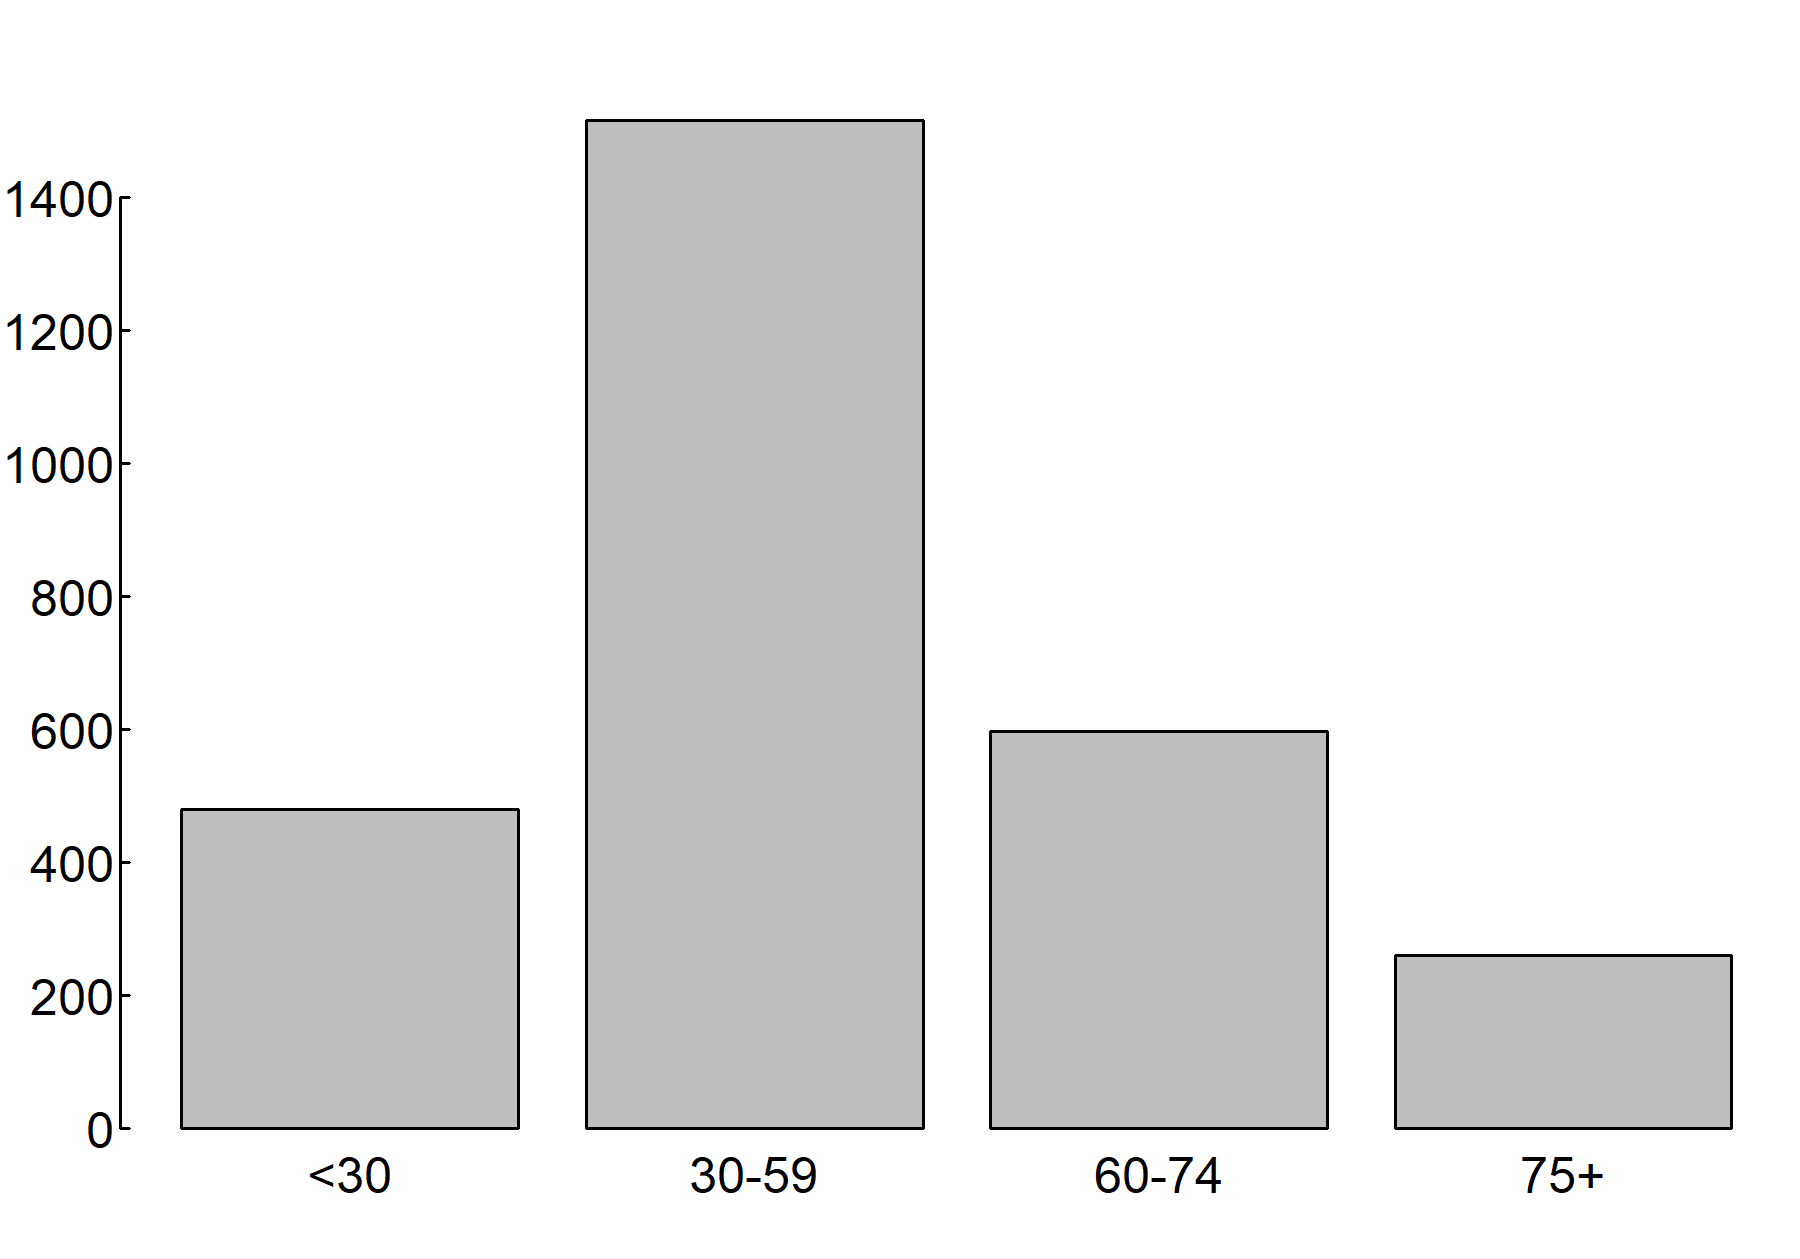
\includegraphics[width=0.6\linewidth]{03_Getting_started_with_a_data_analaysis_files/figure-latex/unnamed-chunk-39-1} \end{center}

where \texttt{gss.2016\$age.f} is a factor.

The values \texttt{table(gss.2016\$age.f)} determine the heights of the bars in the plot, and a vertical bar plot is produced. Including the option \texttt{horiz=TRUE} produces a horizontal bar chart instead. You can also add annotating options. The main option adds a plot title, whereas the xlab and ylab options add x-axis and y-axis labels, respectively.

\begin{Shaded}
\begin{Highlighting}[]
\FunctionTok{par}\NormalTok{(}\AttributeTok{mar =} \FunctionTok{c}\NormalTok{(}\DecValTok{4}\NormalTok{, }\DecValTok{4}\NormalTok{, }\DecValTok{2}\NormalTok{, }\FloatTok{0.1}\NormalTok{), }\AttributeTok{las=}\DecValTok{1}\NormalTok{, }\AttributeTok{mgp=}\FunctionTok{c}\NormalTok{(}\FloatTok{2.5}\NormalTok{,}\FloatTok{0.1}\NormalTok{, }\DecValTok{0}\NormalTok{), }\AttributeTok{tcl=}\FloatTok{0.15}\NormalTok{)}
\NormalTok{counts }\OtherTok{\textless{}{-}} \FunctionTok{table}\NormalTok{(gss}\FloatTok{.2016}\SpecialCharTok{$}\NormalTok{age.f)}
\FunctionTok{barplot}\NormalTok{(counts, }
        \AttributeTok{main=}\StringTok{"Simple Bar Plot"}\NormalTok{, }
        \AttributeTok{xlab=}\StringTok{"Age"}\NormalTok{, }\AttributeTok{ylab=}\StringTok{"Frequency"}\NormalTok{)}
\FunctionTok{barplot}\NormalTok{(counts, }
        \AttributeTok{main=}\StringTok{"Simple Bar Plot"}\NormalTok{, }
        \AttributeTok{xlab=}\StringTok{"Age"}\NormalTok{, }\AttributeTok{ylab=}\StringTok{"Frequency"}\NormalTok{,}
        \AttributeTok{horiz=}\NormalTok{T)}
\end{Highlighting}
\end{Shaded}

\begin{figure}
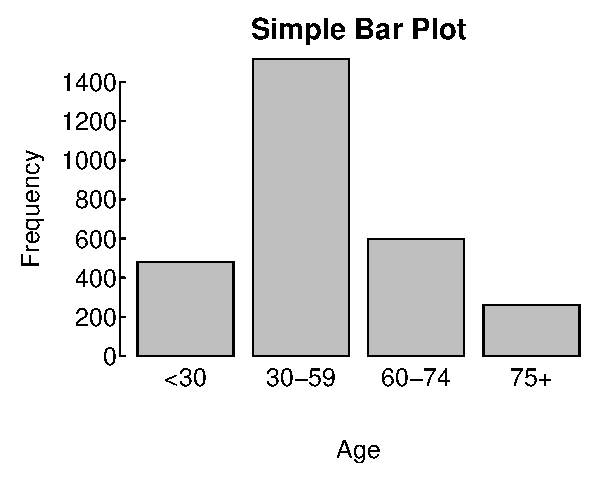
\includegraphics[width=0.5\linewidth]{03_Getting_started_with_a_data_analaysis_files/figure-latex/unnamed-chunk-40-1} 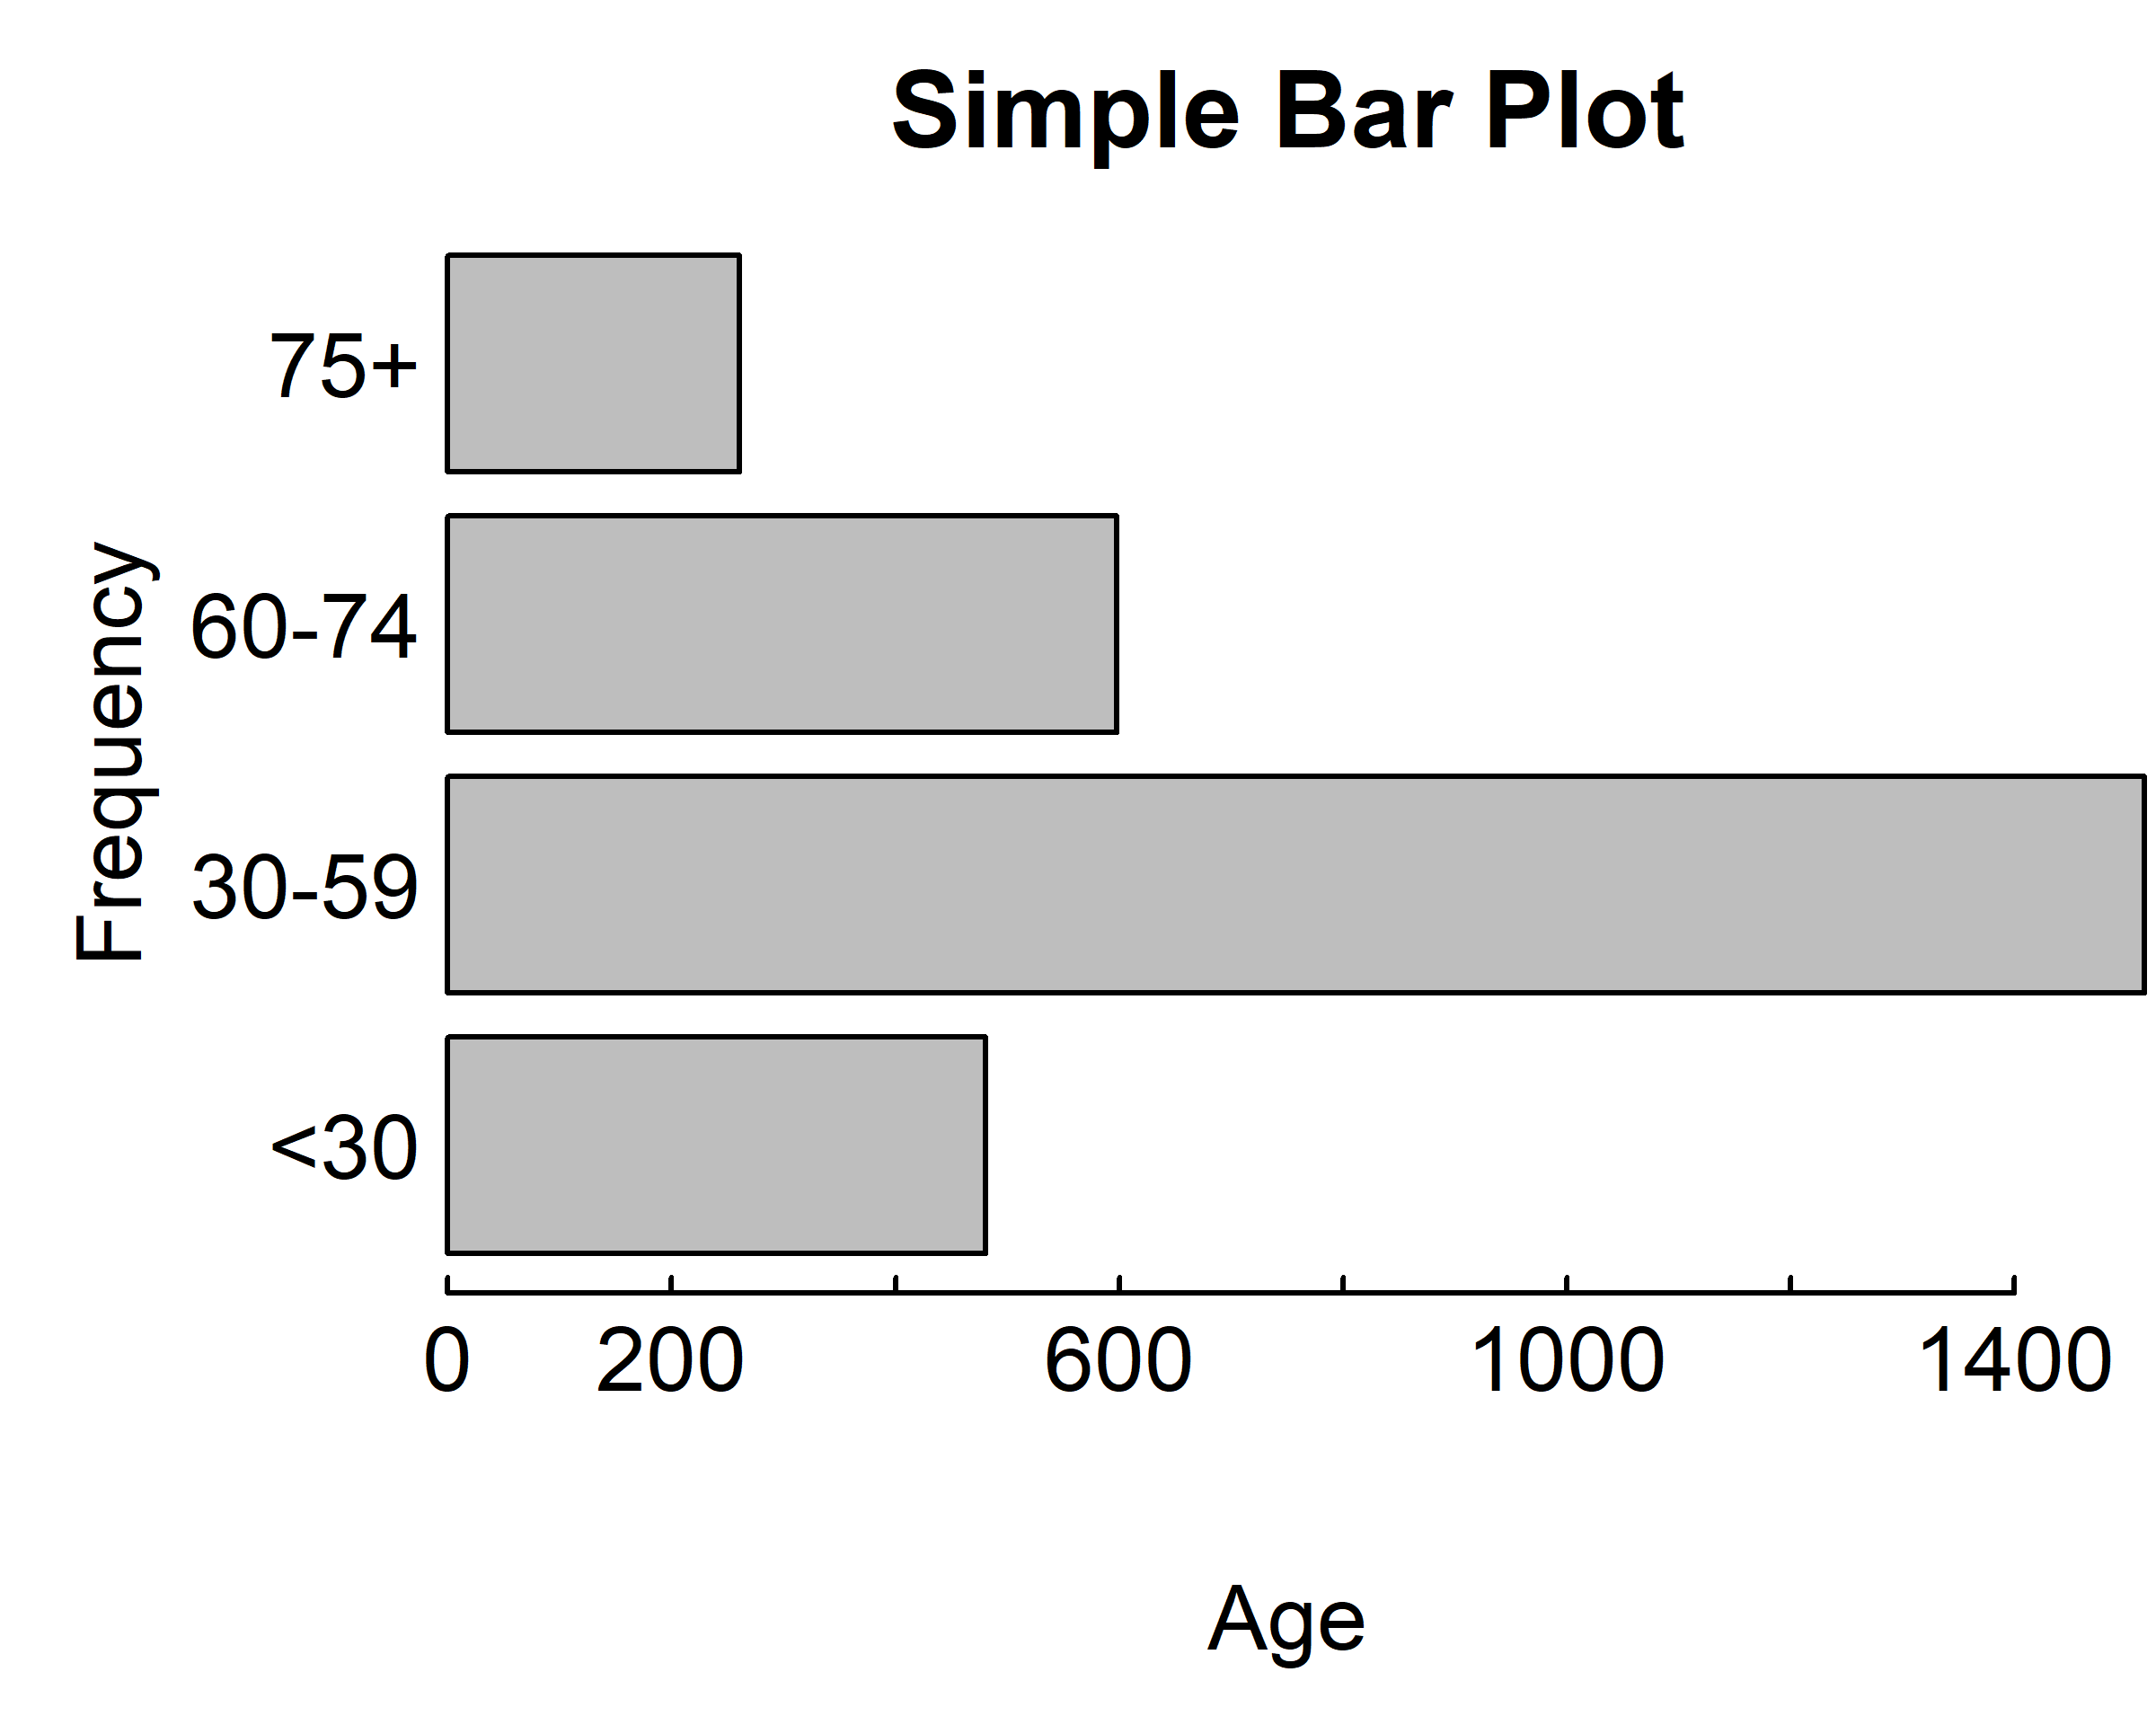
\includegraphics[width=0.5\linewidth]{03_Getting_started_with_a_data_analaysis_files/figure-latex/unnamed-chunk-40-2} \end{figure}

You can customize many features of a graph (fonts, colors, axes, and labels) through options called graphical parameters. One way is to specify these options through the \texttt{par()} function. Values set in this manner will be in effect for the rest of the session or until they're changed. The format is \texttt{par(optionname=value,\ optionname=value,\ ...)}. Specifying \texttt{par()} without parameters produces a list of the current graphical settings.

The relevant parameters are shown below

\begin{longtable}[]{@{}ll@{}}
\toprule
\begin{minipage}[b]{(\columnwidth - 1\tabcolsep) * \real{0.39}}\raggedright
Parameter\strut
\end{minipage} & \begin{minipage}[b]{(\columnwidth - 1\tabcolsep) * \real{0.61}}\raggedright
Description\strut
\end{minipage}\tabularnewline
\midrule
\endhead
\begin{minipage}[t]{(\columnwidth - 1\tabcolsep) * \real{0.39}}\raggedright
\texttt{mar}\strut
\end{minipage} & \begin{minipage}[t]{(\columnwidth - 1\tabcolsep) * \real{0.61}}\raggedright
A numerical vector of the form \texttt{c(bottom,\ left,\ top,\ right)} which gives the number of lines of margin to be specified on the four sides of the plot. The default is \texttt{c(5,\ 4,\ 4,\ 2)\ +\ 0.1}.\strut
\end{minipage}\tabularnewline
\begin{minipage}[t]{(\columnwidth - 1\tabcolsep) * \real{0.39}}\raggedright
\texttt{las}\strut
\end{minipage} & \begin{minipage}[t]{(\columnwidth - 1\tabcolsep) * \real{0.61}}\raggedright
Specifies that labels are parallel (= 0) or perpendicular (= 2) to the axis.\strut
\end{minipage}\tabularnewline
\begin{minipage}[t]{(\columnwidth - 1\tabcolsep) * \real{0.39}}\raggedright
\texttt{tck}\strut
\end{minipage} & \begin{minipage}[t]{(\columnwidth - 1\tabcolsep) * \real{0.61}}\raggedright
Length of each tick mark as a fraction of the plotting region (a negative number is outside the graph, a positive number is inside, 0 suppresses ticks, and 1 creates gridlines). The default is -0.01.\strut
\end{minipage}\tabularnewline
\begin{minipage}[t]{(\columnwidth - 1\tabcolsep) * \real{0.39}}\raggedright
\texttt{mgp}\strut
\end{minipage} & \begin{minipage}[t]{(\columnwidth - 1\tabcolsep) * \real{0.61}}\raggedright
The margin line for the axis title, axis labels and axis line. Note that \texttt{mgp{[}1{]}} affects title whereas \texttt{mgp{[}2:3{]}} affect axis. The default is \texttt{c(3,\ 1,\ 0)}.\strut
\end{minipage}\tabularnewline
\bottomrule
\end{longtable}

If the argument of \texttt{barplot()} is a matrix rather than a vector, the resulting graph will be a stacked or grouped bar plot. If \texttt{beside=FALSE} (the default), then each column of the matrix produces a bar in the plot, with the values in the column giving the heights of stacked ``sub-bars.'' If \texttt{beside=TRUE}, each column of the matrix represents a group, and the values in each column are juxtaposed rather than stacked.

Consider the cross-tabulation of age and votes:

\begin{Shaded}
\begin{Highlighting}[]
\NormalTok{counts }\OtherTok{\textless{}{-}} \FunctionTok{table}\NormalTok{(gss}\FloatTok{.2016}\SpecialCharTok{$}\NormalTok{grass, gss}\FloatTok{.2016}\SpecialCharTok{$}\NormalTok{age.f)}
\NormalTok{counts}
\CommentTok{\#\textgreater{}            }
\CommentTok{\#\textgreater{}             \textless{}30 30{-}59 60{-}74 75+}
\CommentTok{\#\textgreater{}   LEGAL     237   625   213  48}
\CommentTok{\#\textgreater{}   NOT LEGAL  95   364   151 103}
\end{Highlighting}
\end{Shaded}

You can graph the results as either a stacked or a grouped bar plot. The resulting graphs are displayed below

\begin{Shaded}
\begin{Highlighting}[]
\FunctionTok{par}\NormalTok{(}\AttributeTok{mar =} \FunctionTok{c}\NormalTok{(}\DecValTok{4}\NormalTok{, }\DecValTok{4}\NormalTok{, }\DecValTok{2}\NormalTok{, }\FloatTok{0.1}\NormalTok{), }\AttributeTok{las=}\DecValTok{1}\NormalTok{, }\AttributeTok{mgp=}\FunctionTok{c}\NormalTok{(}\FloatTok{2.5}\NormalTok{,}\FloatTok{0.1}\NormalTok{, }\DecValTok{0}\NormalTok{), }\AttributeTok{tcl=}\FloatTok{0.15}\NormalTok{)}
\FunctionTok{barplot}\NormalTok{(counts, }
        \AttributeTok{main=}\StringTok{"Stacked Bar Plot"}\NormalTok{, }
        \AttributeTok{xlab=}\StringTok{"Age"}\NormalTok{, }\AttributeTok{ylab=}\StringTok{"Frequency"}\NormalTok{,}
        \AttributeTok{col=}\FunctionTok{c}\NormalTok{(}\StringTok{"lightgreen"}\NormalTok{, }\StringTok{"red"}\NormalTok{),}
        \AttributeTok{legend=}\NormalTok{T)}
\FunctionTok{barplot}\NormalTok{(counts, }
        \AttributeTok{main=}\StringTok{"Stacked Bar Plot"}\NormalTok{, }
        \AttributeTok{xlab=}\StringTok{"Age"}\NormalTok{, }\AttributeTok{ylab=}\StringTok{"Frequency"}\NormalTok{,}
        \AttributeTok{col=}\FunctionTok{c}\NormalTok{(}\StringTok{"lightgreen"}\NormalTok{, }\StringTok{"red"}\NormalTok{),}
        \AttributeTok{legend=}\NormalTok{T, }\AttributeTok{beside =}\NormalTok{ T)}
\end{Highlighting}
\end{Shaded}

\begin{figure}
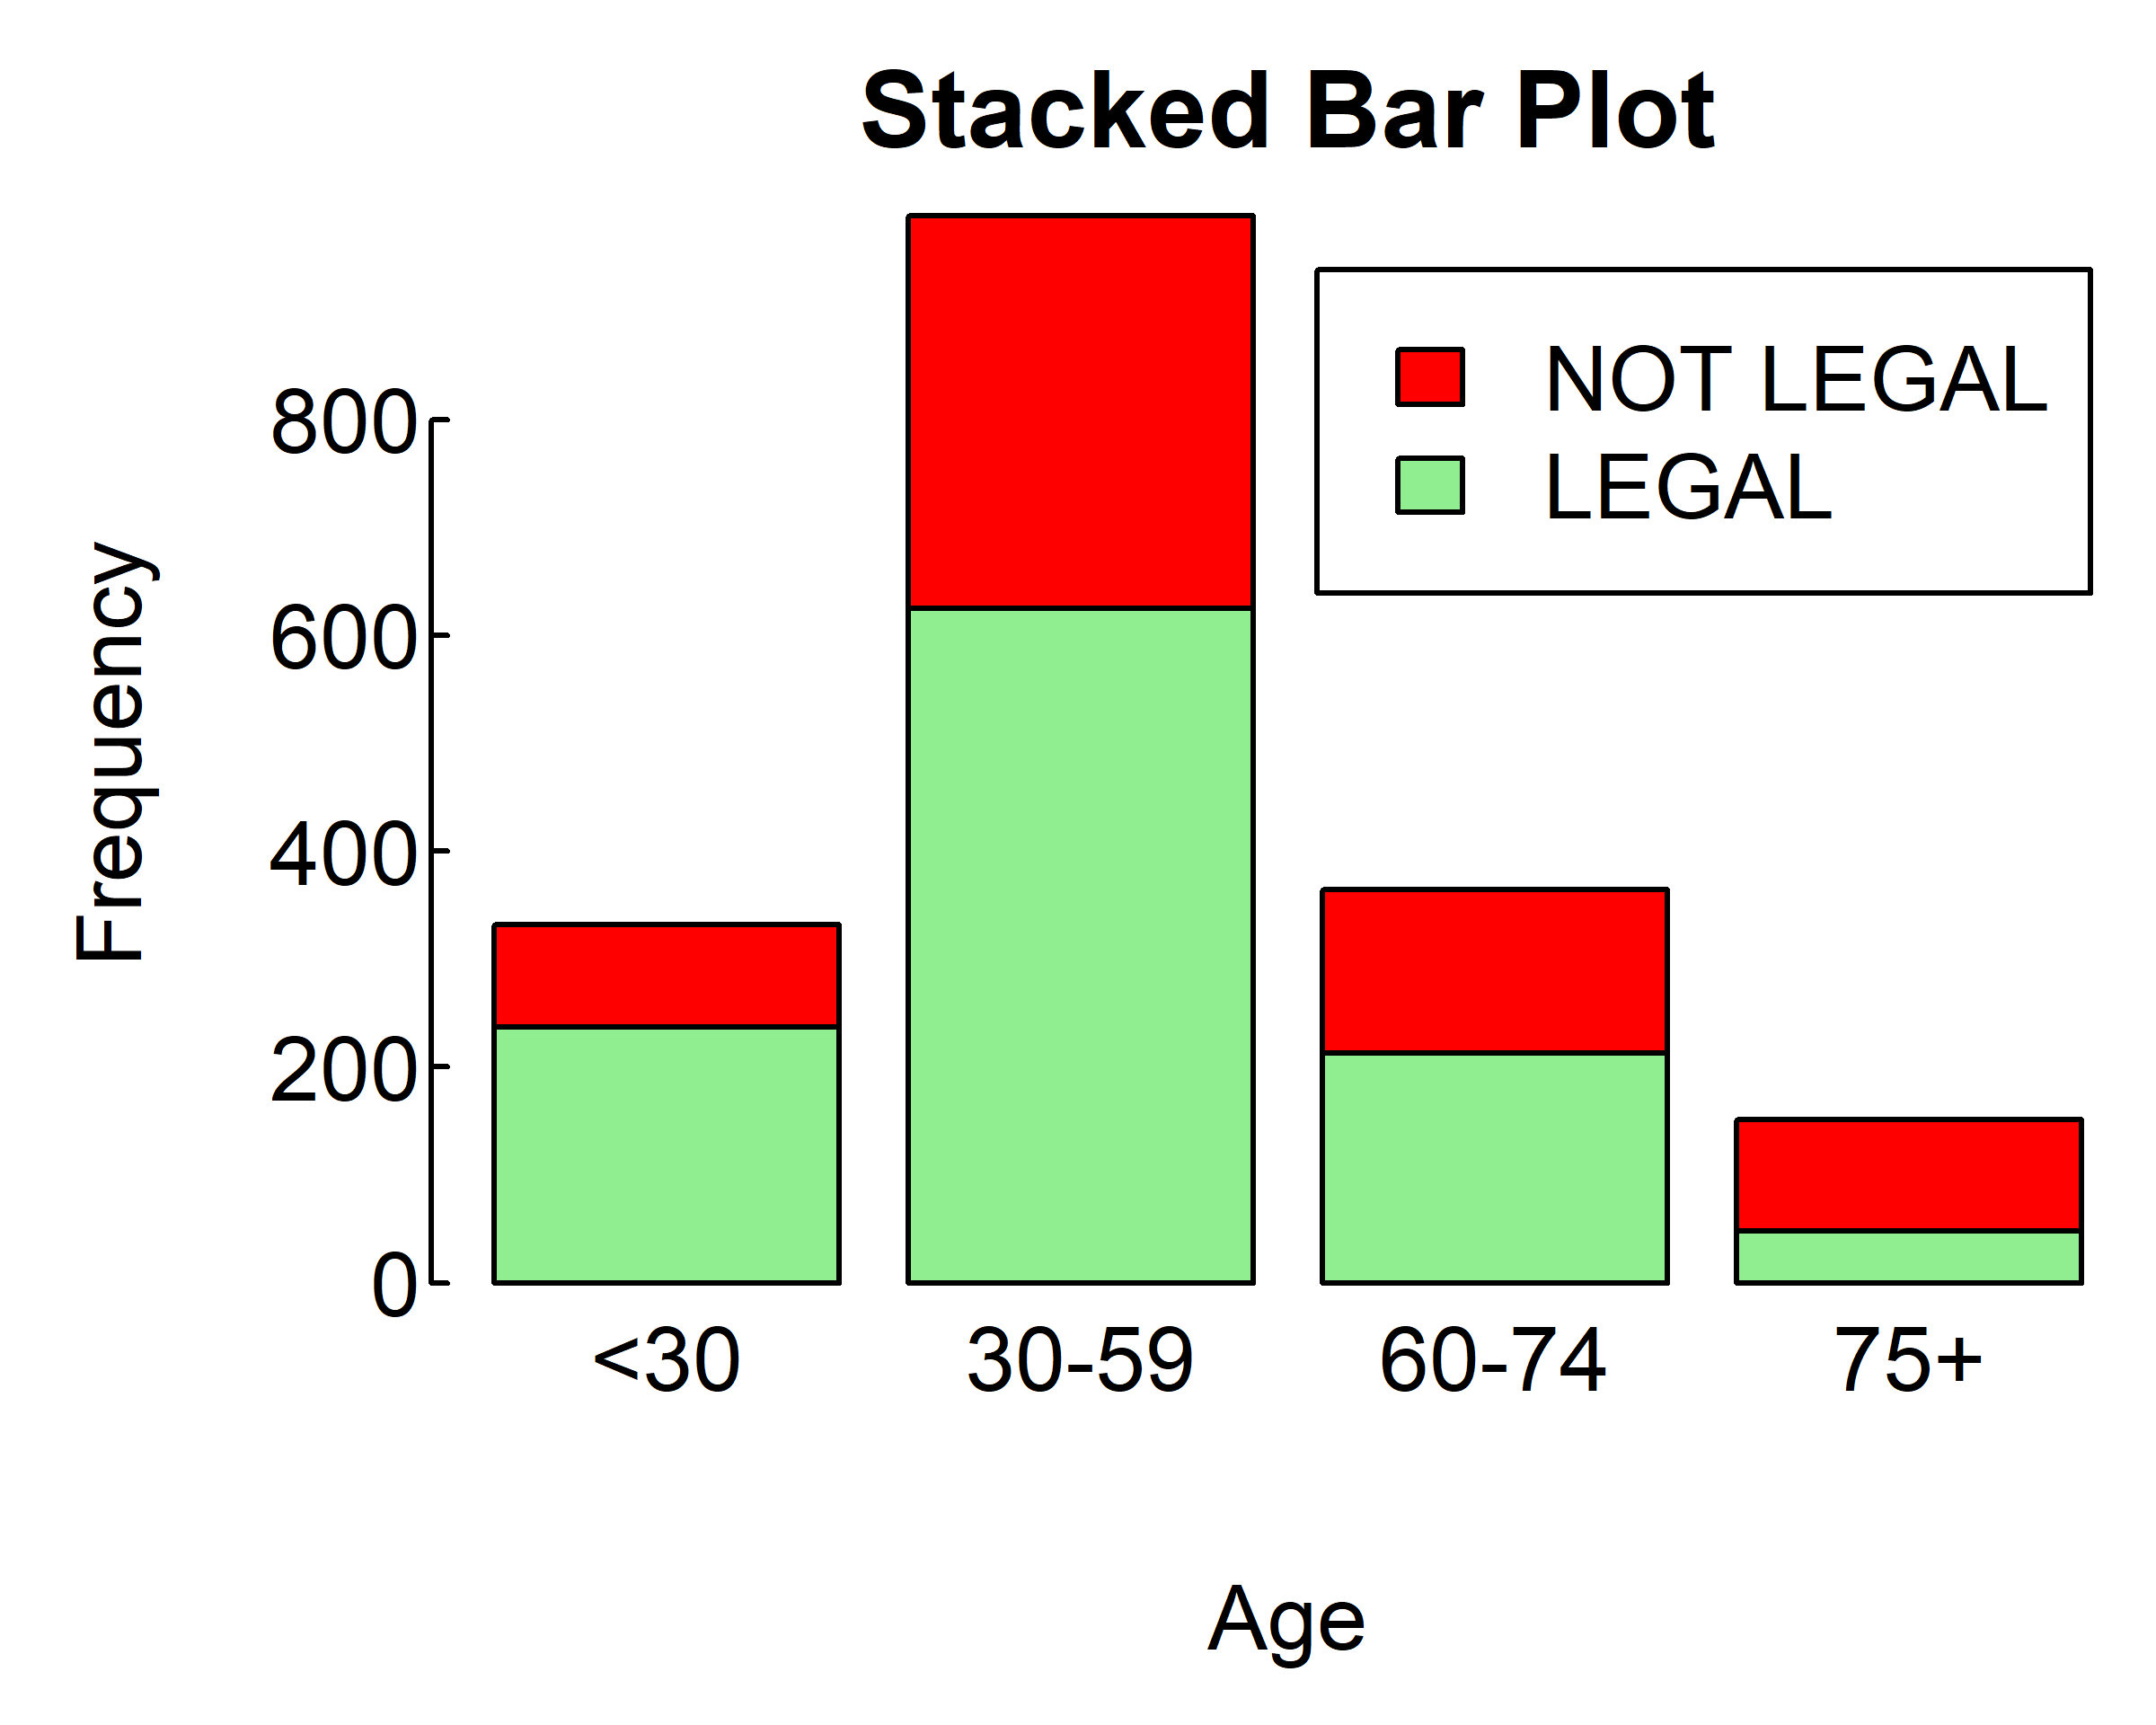
\includegraphics[width=0.5\linewidth]{03_Getting_started_with_a_data_analaysis_files/figure-latex/unnamed-chunk-42-1} 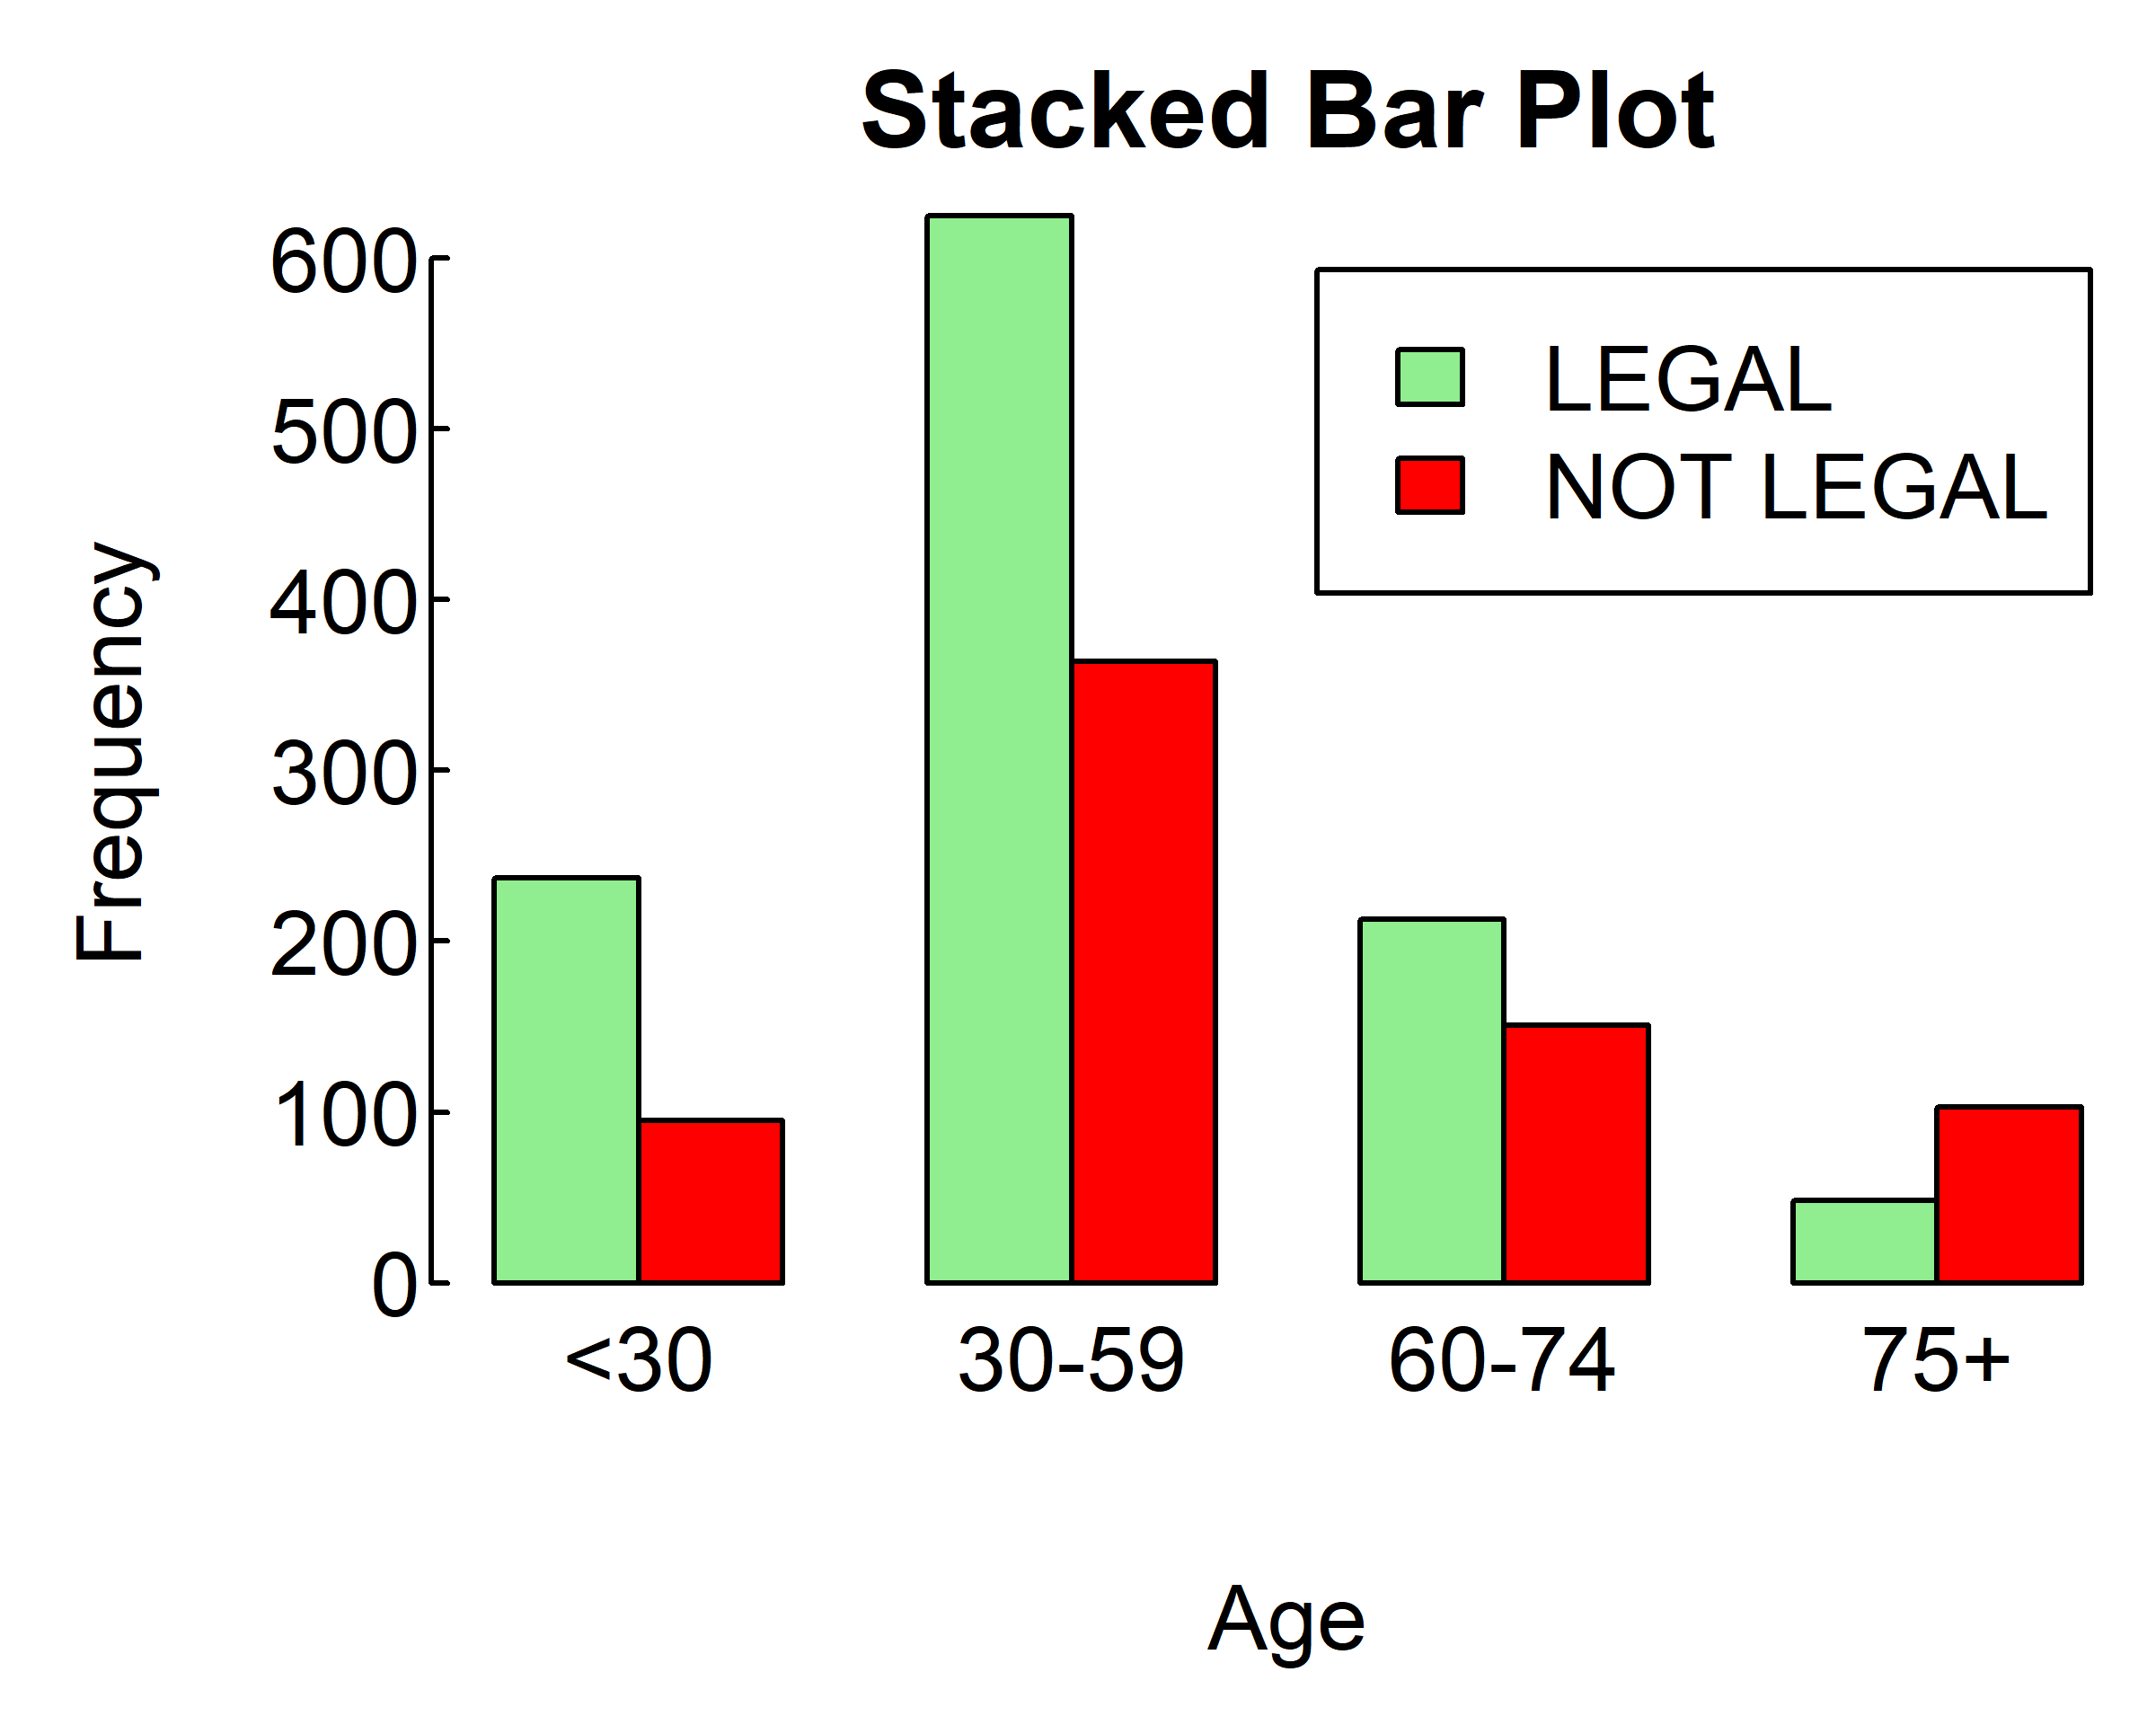
\includegraphics[width=0.5\linewidth]{03_Getting_started_with_a_data_analaysis_files/figure-latex/unnamed-chunk-42-2} \end{figure}

Bar plots needn't be based on counts or frequencies. You can create bar plots that represent means, medians, standard deviations, and so forth by using the aggregate function and passing the results to the \texttt{barplot()} function. The following listing shows an example, which is displayed below.

\begin{Shaded}
\begin{Highlighting}[]
\FunctionTok{par}\NormalTok{(}\AttributeTok{mar =} \FunctionTok{c}\NormalTok{(}\DecValTok{4}\NormalTok{, }\DecValTok{4}\NormalTok{, }\DecValTok{2}\NormalTok{, }\FloatTok{0.1}\NormalTok{), }\AttributeTok{las=}\DecValTok{1}\NormalTok{, }\AttributeTok{mgp=}\FunctionTok{c}\NormalTok{(}\FloatTok{2.5}\NormalTok{,}\FloatTok{0.1}\NormalTok{, }\DecValTok{0}\NormalTok{), }\AttributeTok{tcl=}\FloatTok{0.15}\NormalTok{)}
\NormalTok{means }\OtherTok{\textless{}{-}} \FunctionTok{aggregate}\NormalTok{(survey}\SpecialCharTok{$}\NormalTok{Height, }
\NormalTok{                   survey[,}\StringTok{"Sex"}\NormalTok{,}\AttributeTok{drop=}\NormalTok{F], mean, }\AttributeTok{na.rm=}\NormalTok{T)}
\NormalTok{means}
\CommentTok{\#\textgreater{}      Sex        x}
\CommentTok{\#\textgreater{} 1 Female 165.6867}
\CommentTok{\#\textgreater{} 2   Male 178.8260}
\FunctionTok{barplot}\NormalTok{(means}\SpecialCharTok{$}\NormalTok{x, }\AttributeTok{names.arg =}\NormalTok{ means}\SpecialCharTok{$}\NormalTok{Sex, }
        \AttributeTok{main=}\StringTok{"Mean height"}\NormalTok{)}
\FunctionTok{barplot}\NormalTok{(means}\SpecialCharTok{$}\NormalTok{x, }\AttributeTok{names.arg =}\NormalTok{ means}\SpecialCharTok{$}\NormalTok{Sex, }
        \AttributeTok{main=}\StringTok{"Mean height"}\NormalTok{, }\AttributeTok{horiz =}\NormalTok{ T)}
\end{Highlighting}
\end{Shaded}

\begin{figure}
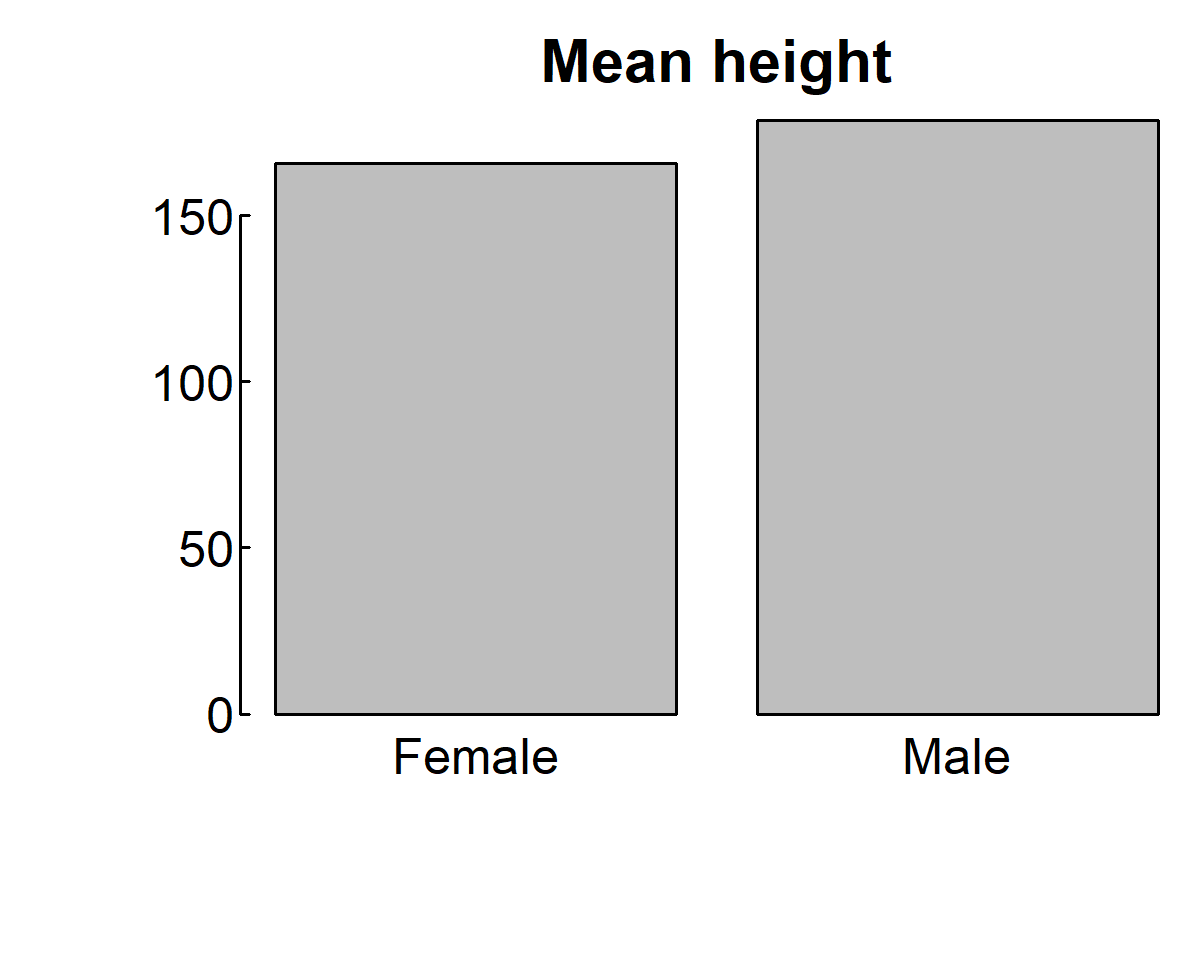
\includegraphics[width=0.5\linewidth]{03_Getting_started_with_a_data_analaysis_files/figure-latex/unnamed-chunk-43-1} 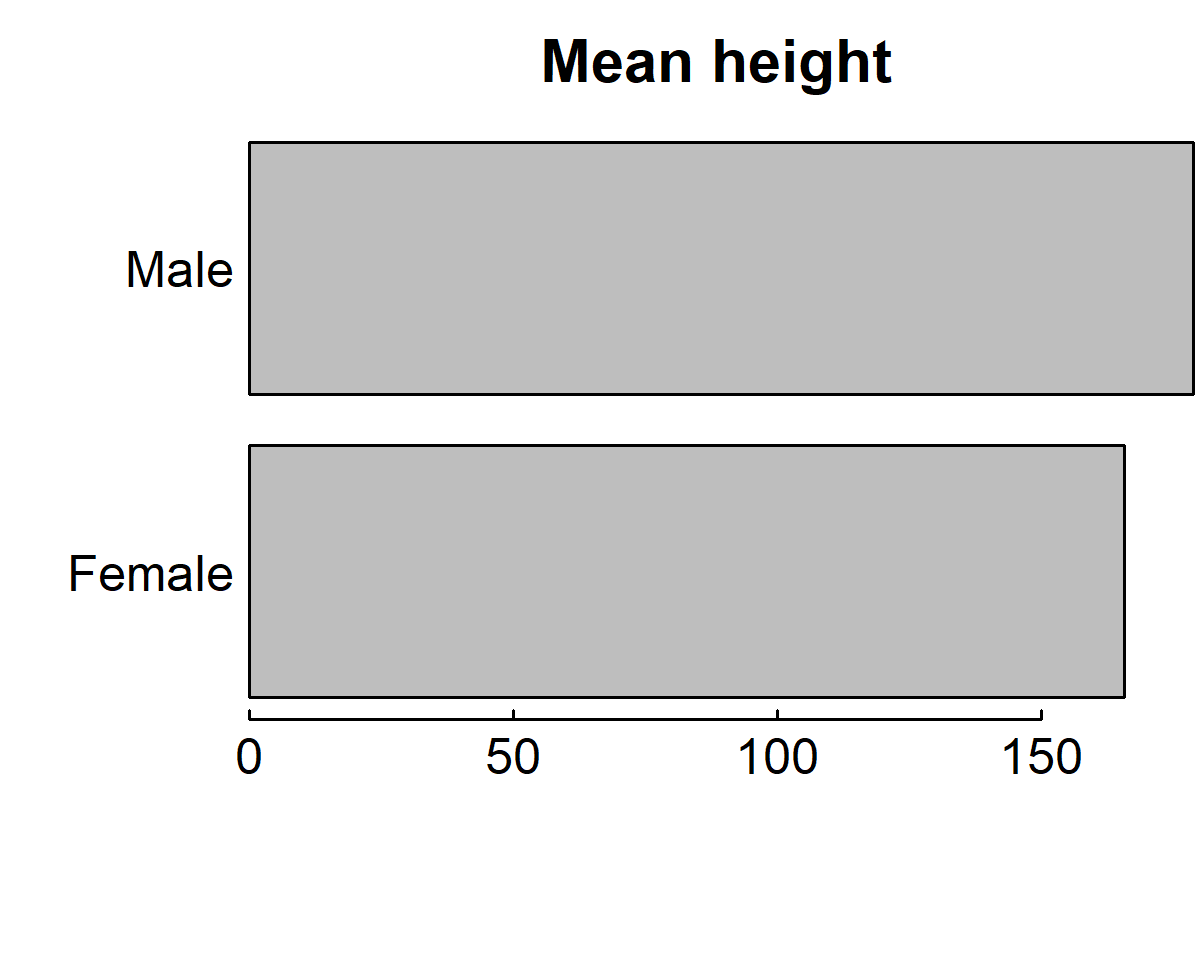
\includegraphics[width=0.5\linewidth]{03_Getting_started_with_a_data_analaysis_files/figure-latex/unnamed-chunk-43-2} \end{figure}

\texttt{means\$x} is the vector containing the heights of the bars, and the option \texttt{names.arg=means\$Sex} is added to provide labels.

Please study carefully the following codes and outputs:

\begin{Shaded}
\begin{Highlighting}[]
\FunctionTok{par}\NormalTok{(}\AttributeTok{mar =} \FunctionTok{c}\NormalTok{(}\DecValTok{4}\NormalTok{, }\DecValTok{4}\NormalTok{, }\DecValTok{2}\NormalTok{, }\FloatTok{0.1}\NormalTok{), }\AttributeTok{las=}\DecValTok{1}\NormalTok{, }\AttributeTok{mgp=}\FunctionTok{c}\NormalTok{(}\FloatTok{2.5}\NormalTok{,}\FloatTok{0.1}\NormalTok{, }\DecValTok{0}\NormalTok{), }\AttributeTok{tcl=}\FloatTok{0.15}\NormalTok{)}
\FunctionTok{barplot}\NormalTok{(}\FunctionTok{table}\NormalTok{(gss}\FloatTok{.2016}\SpecialCharTok{$}\NormalTok{age.f))}
\FunctionTok{barplot}\NormalTok{(}\FunctionTok{table}\NormalTok{(gss}\FloatTok{.2016}\SpecialCharTok{$}\NormalTok{grass))}

\FunctionTok{barplot}\NormalTok{(}\FunctionTok{table}\NormalTok{(gss}\FloatTok{.2016}\SpecialCharTok{$}\NormalTok{grass), }\AttributeTok{col=}\FunctionTok{c}\NormalTok{(}\StringTok{"green"}\NormalTok{, }\StringTok{"purple"}\NormalTok{))}
\FunctionTok{barplot}\NormalTok{(}\FunctionTok{table}\NormalTok{(gss}\FloatTok{.2016}\SpecialCharTok{$}\NormalTok{grass), }\AttributeTok{col=}\FunctionTok{c}\NormalTok{(}\StringTok{"\#78A678"}\NormalTok{, }\StringTok{"\#7463AC"}\NormalTok{))}
\FunctionTok{barplot}\NormalTok{(}\FunctionTok{table}\NormalTok{(gss}\FloatTok{.2016}\SpecialCharTok{$}\NormalTok{grass), }\AttributeTok{col=}\FunctionTok{c}\NormalTok{(}\StringTok{"\#78A678"}\NormalTok{, }\StringTok{"\#7463AC"}\NormalTok{),}
\AttributeTok{xlab=}\StringTok{"Should marijuana be legal?"}\NormalTok{, }\AttributeTok{ylab=}\StringTok{"Number of responses"}\NormalTok{)}

\FunctionTok{par}\NormalTok{(}\AttributeTok{las=}\DecValTok{1}\NormalTok{, }\AttributeTok{mgp=}\FunctionTok{c}\NormalTok{(}\DecValTok{2}\NormalTok{,}\FloatTok{0.2}\NormalTok{,}\DecValTok{0}\NormalTok{), }\AttributeTok{tcl=}\FloatTok{0.1}\NormalTok{, }\AttributeTok{mar=}\FunctionTok{c}\NormalTok{(}\DecValTok{2}\NormalTok{,}\DecValTok{3}\NormalTok{,}\DecValTok{1}\NormalTok{,}\DecValTok{1}\NormalTok{))}
\FunctionTok{barplot}\NormalTok{(}\FunctionTok{table}\NormalTok{(gss}\FloatTok{.2016}\SpecialCharTok{$}\NormalTok{grass), }\AttributeTok{col=}\FunctionTok{c}\NormalTok{(}\StringTok{"\#78A678"}\NormalTok{, }\StringTok{"\#7463AC"}\NormalTok{),}
\AttributeTok{xlab=}\StringTok{"Should marijuana be legal?"}\NormalTok{, }\AttributeTok{ylab=}\StringTok{"Number of responses"}\NormalTok{)}

\CommentTok{\# to save plot to PNG}
\FunctionTok{par}\NormalTok{(}\AttributeTok{las=}\DecValTok{1}\NormalTok{, }\AttributeTok{mgp=}\FunctionTok{c}\NormalTok{(}\DecValTok{2}\NormalTok{,}\FloatTok{0.2}\NormalTok{,}\DecValTok{0}\NormalTok{), }\AttributeTok{tcl=}\FloatTok{0.1}\NormalTok{, }\AttributeTok{mar=}\FunctionTok{c}\NormalTok{(}\DecValTok{2}\NormalTok{,}\DecValTok{3}\NormalTok{,}\DecValTok{1}\NormalTok{,}\DecValTok{1}\NormalTok{))}
\FunctionTok{barplot}\NormalTok{(}\FunctionTok{table}\NormalTok{(gss}\FloatTok{.2016}\SpecialCharTok{$}\NormalTok{grass, gss}\FloatTok{.2016}\SpecialCharTok{$}\NormalTok{age.f), }\AttributeTok{beside =}\NormalTok{ T, }\AttributeTok{legend=}\NormalTok{T)}

\FunctionTok{png}\NormalTok{(}\AttributeTok{filename =} \StringTok{"output/image/barplot\_1.png"}\NormalTok{, }\AttributeTok{width =} \DecValTok{400}\NormalTok{, }\AttributeTok{height =} \DecValTok{300}\NormalTok{)}
\FunctionTok{par}\NormalTok{(}\AttributeTok{las=}\DecValTok{1}\NormalTok{, }\AttributeTok{mgp=}\FunctionTok{c}\NormalTok{(}\DecValTok{2}\NormalTok{,}\FloatTok{0.2}\NormalTok{,}\DecValTok{0}\NormalTok{), }\AttributeTok{tcl=}\FloatTok{0.1}\NormalTok{, }\AttributeTok{mar=}\FunctionTok{c}\NormalTok{(}\DecValTok{2}\NormalTok{,}\DecValTok{3}\NormalTok{,}\DecValTok{1}\NormalTok{,}\DecValTok{1}\NormalTok{))}
\FunctionTok{barplot}\NormalTok{(}\FunctionTok{table}\NormalTok{(gss}\FloatTok{.2016}\SpecialCharTok{$}\NormalTok{grass, gss}\FloatTok{.2016}\SpecialCharTok{$}\NormalTok{age.f), }\AttributeTok{beside =}\NormalTok{ T, }\AttributeTok{legend=}\NormalTok{T)}
\FunctionTok{dev.off}\NormalTok{()}
\CommentTok{\#\textgreater{} pdf }
\CommentTok{\#\textgreater{}   2}
\end{Highlighting}
\end{Shaded}

\begin{figure}
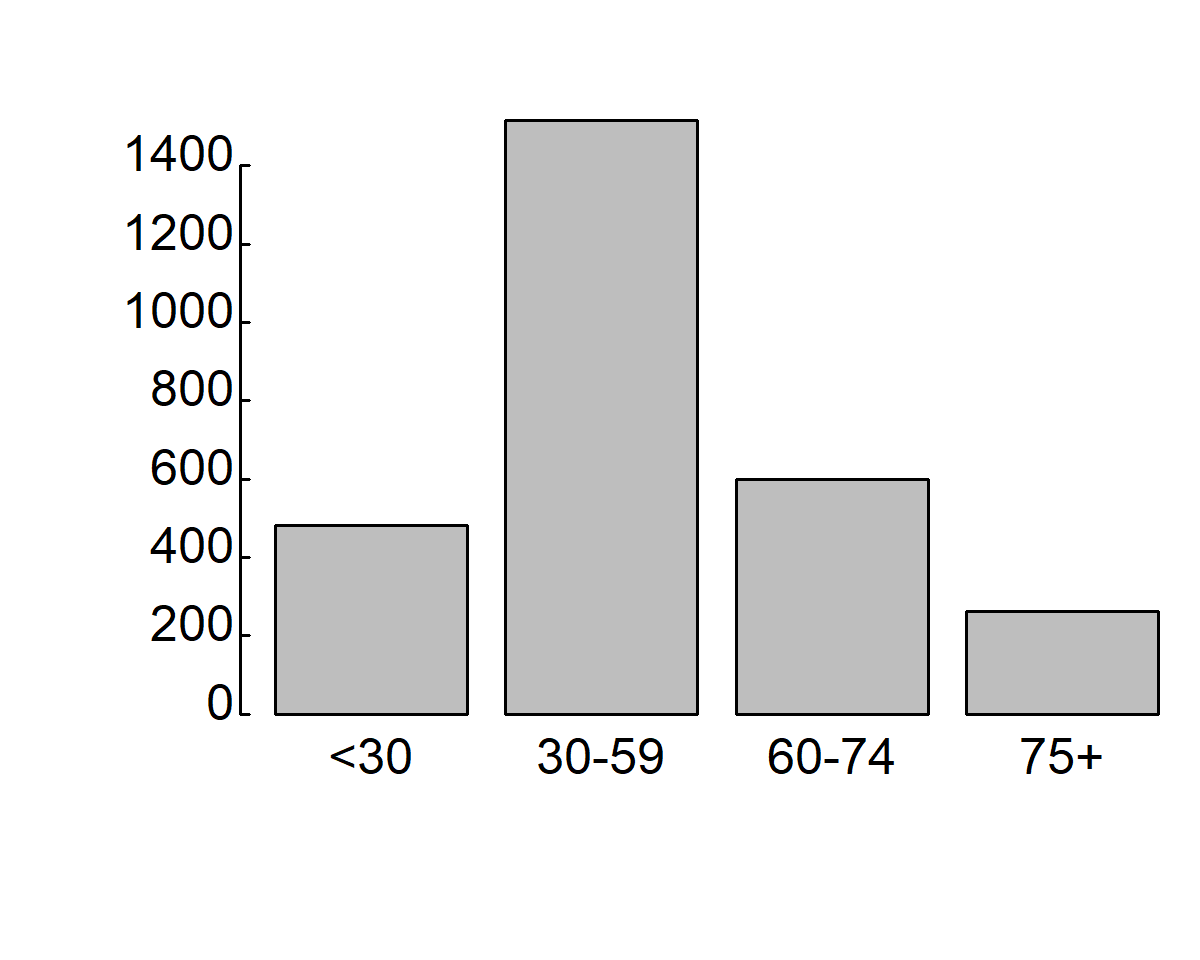
\includegraphics[width=0.5\linewidth]{03_Getting_started_with_a_data_analaysis_files/figure-latex/unnamed-chunk-44-1} 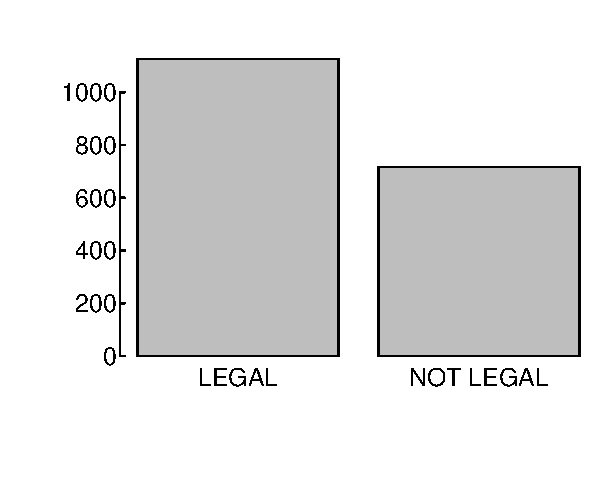
\includegraphics[width=0.5\linewidth]{03_Getting_started_with_a_data_analaysis_files/figure-latex/unnamed-chunk-44-2} 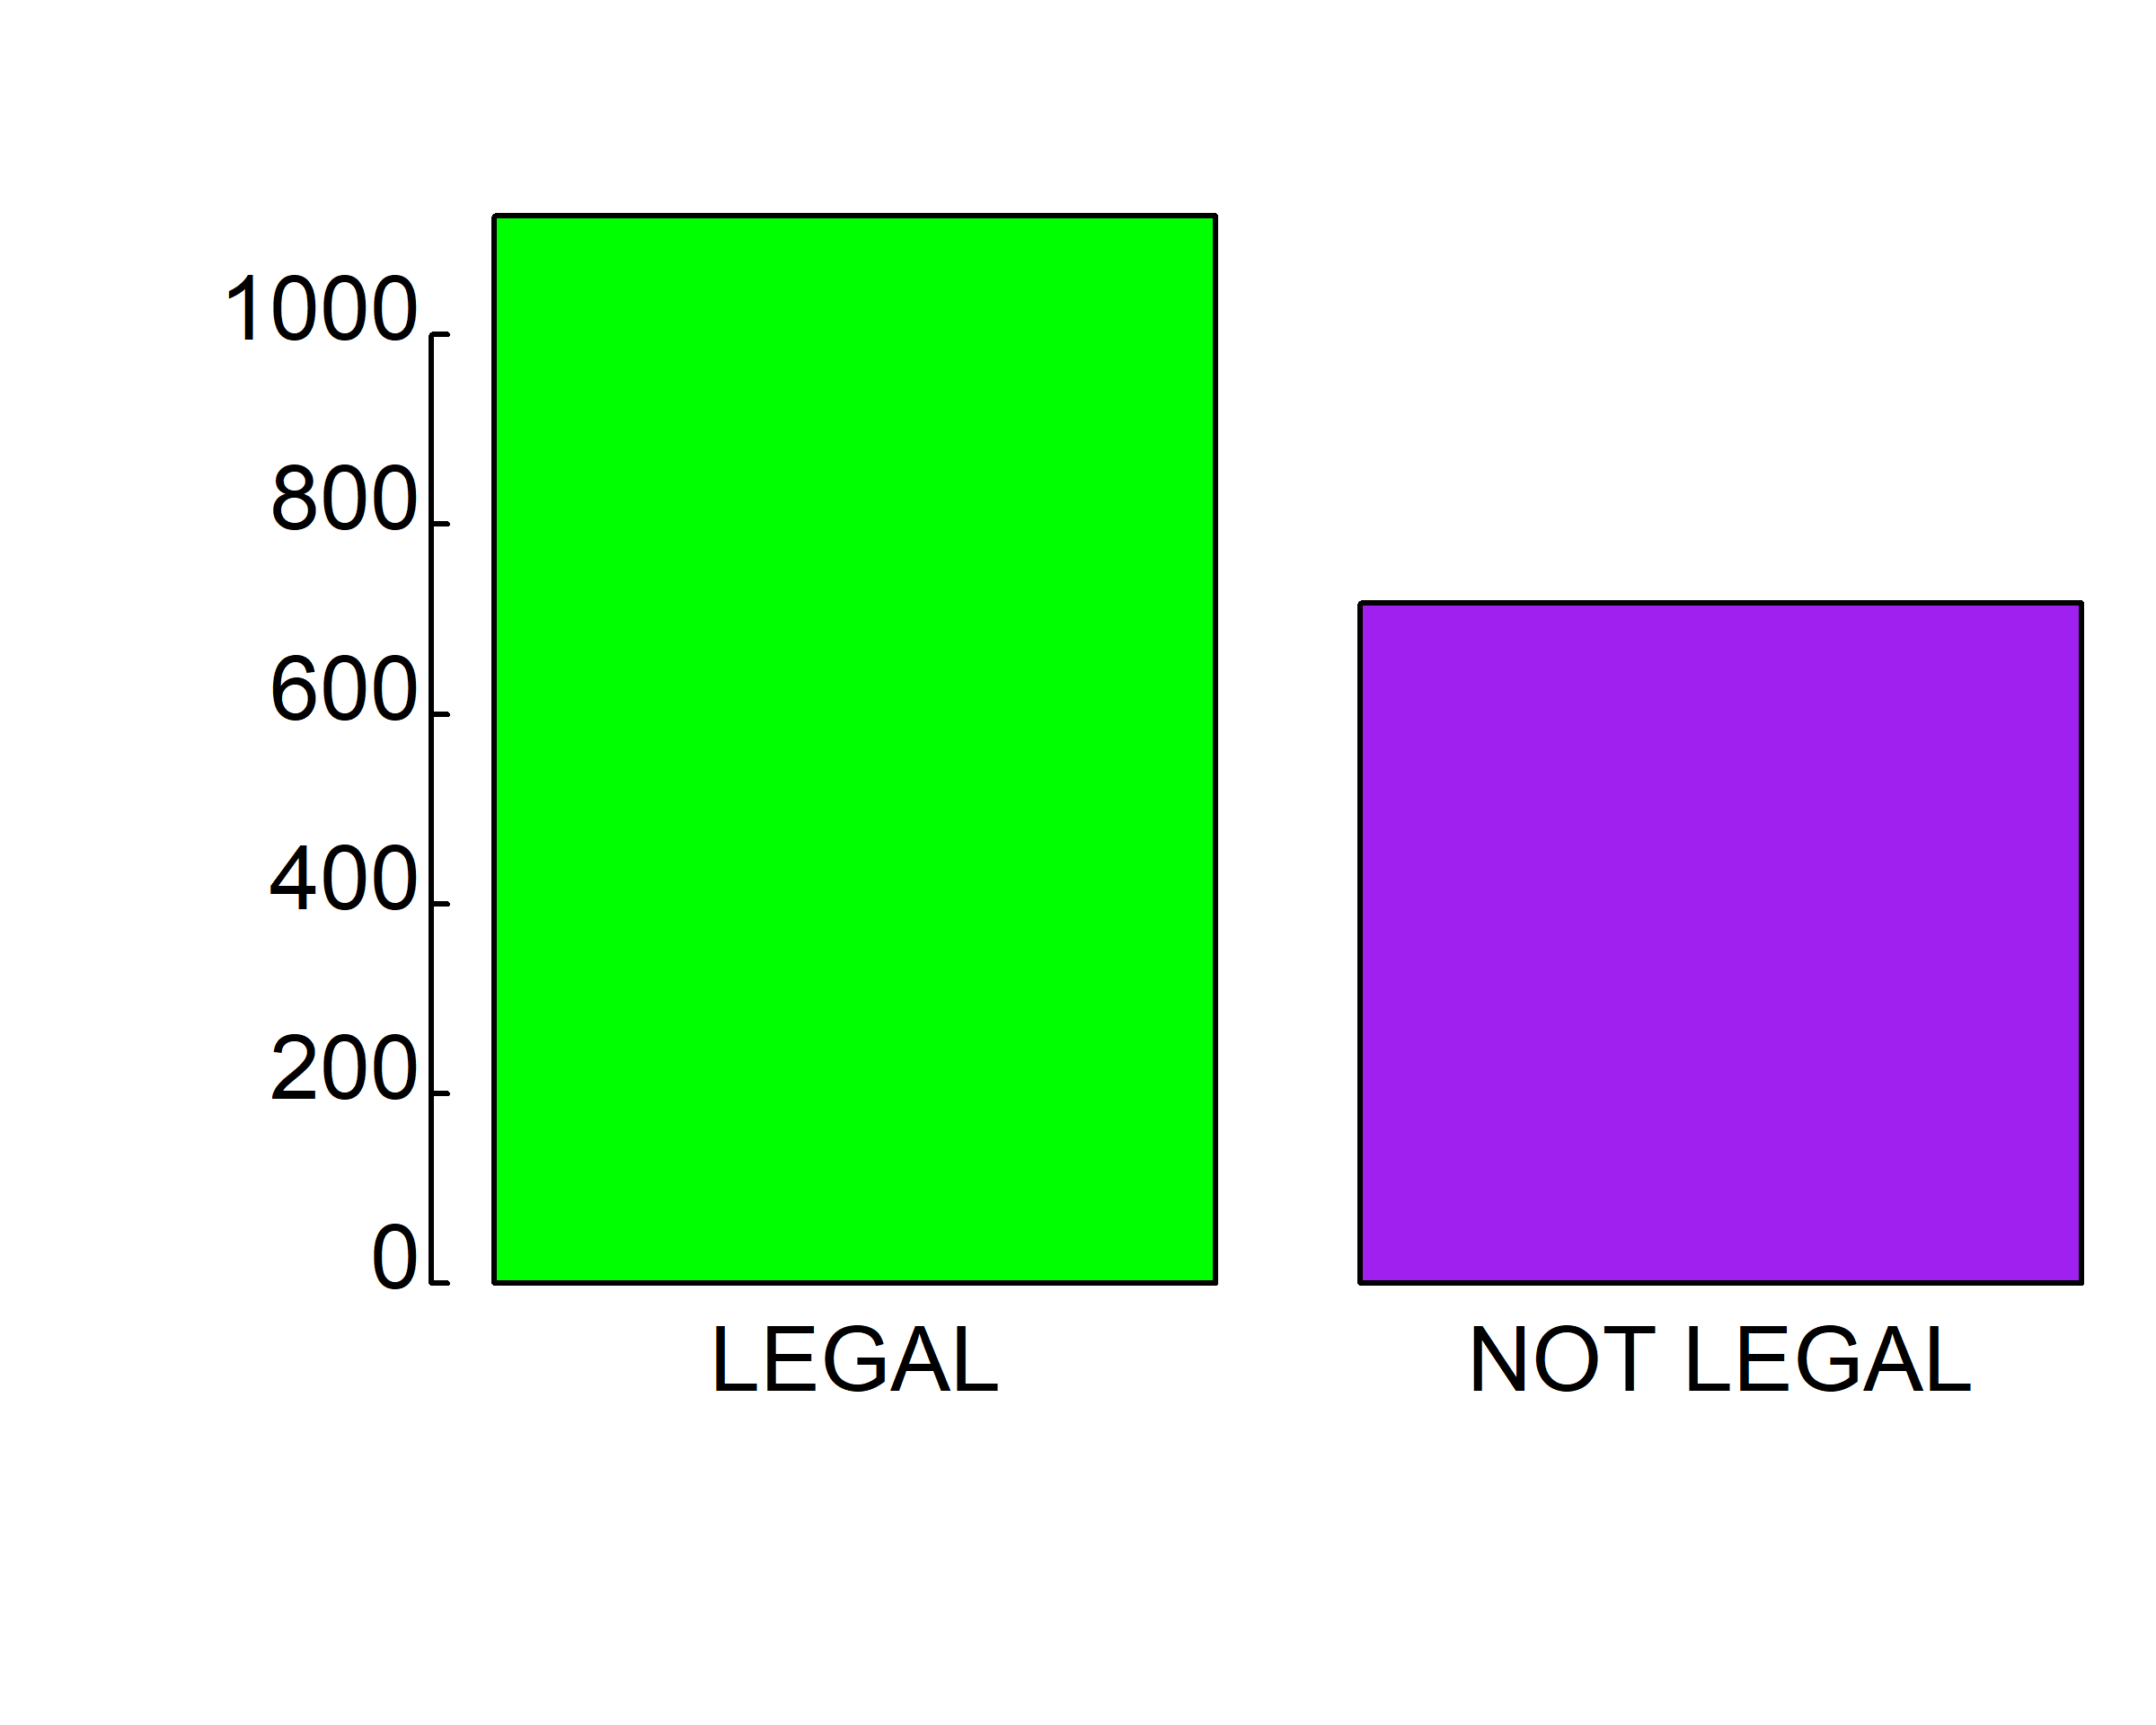
\includegraphics[width=0.5\linewidth]{03_Getting_started_with_a_data_analaysis_files/figure-latex/unnamed-chunk-44-3} 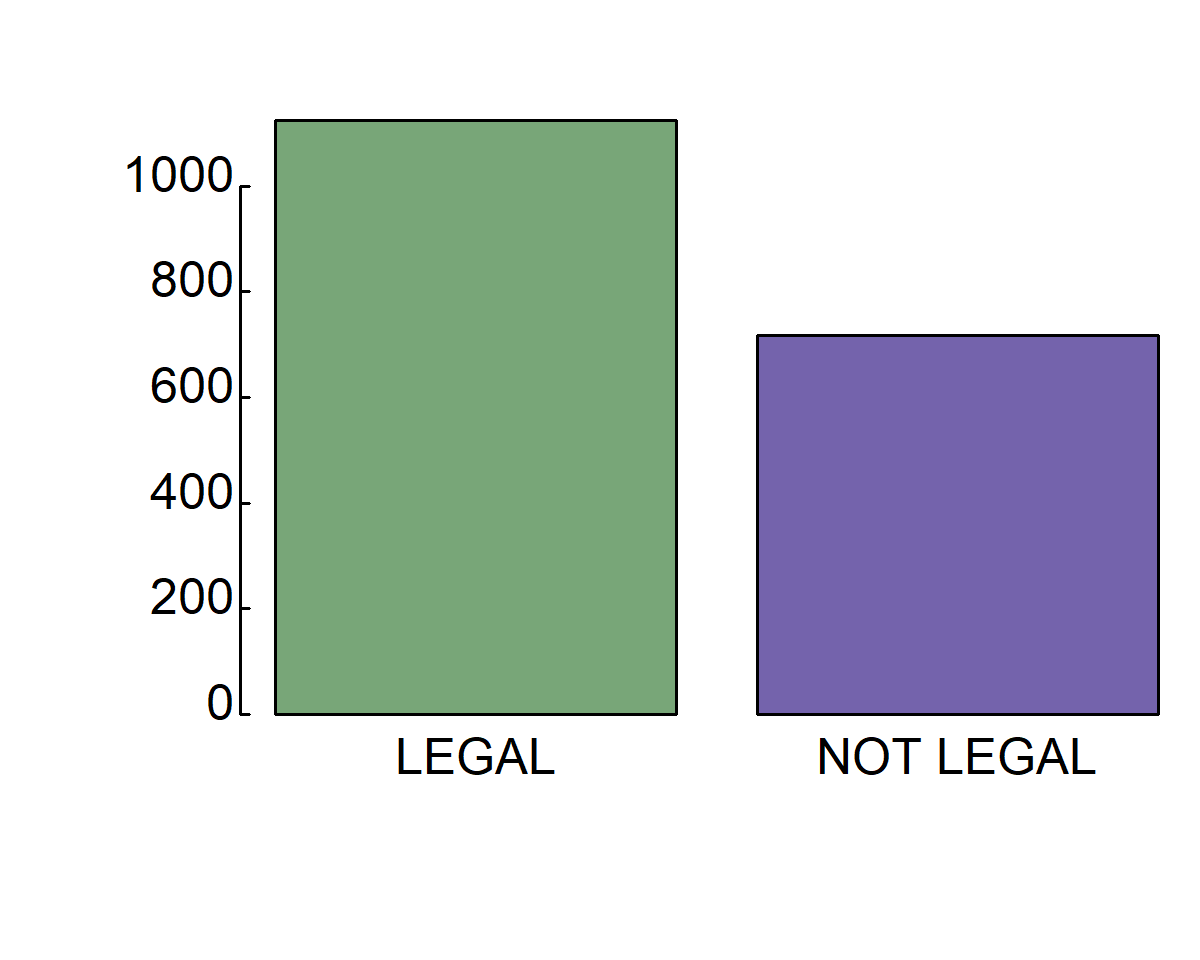
\includegraphics[width=0.5\linewidth]{03_Getting_started_with_a_data_analaysis_files/figure-latex/unnamed-chunk-44-4} 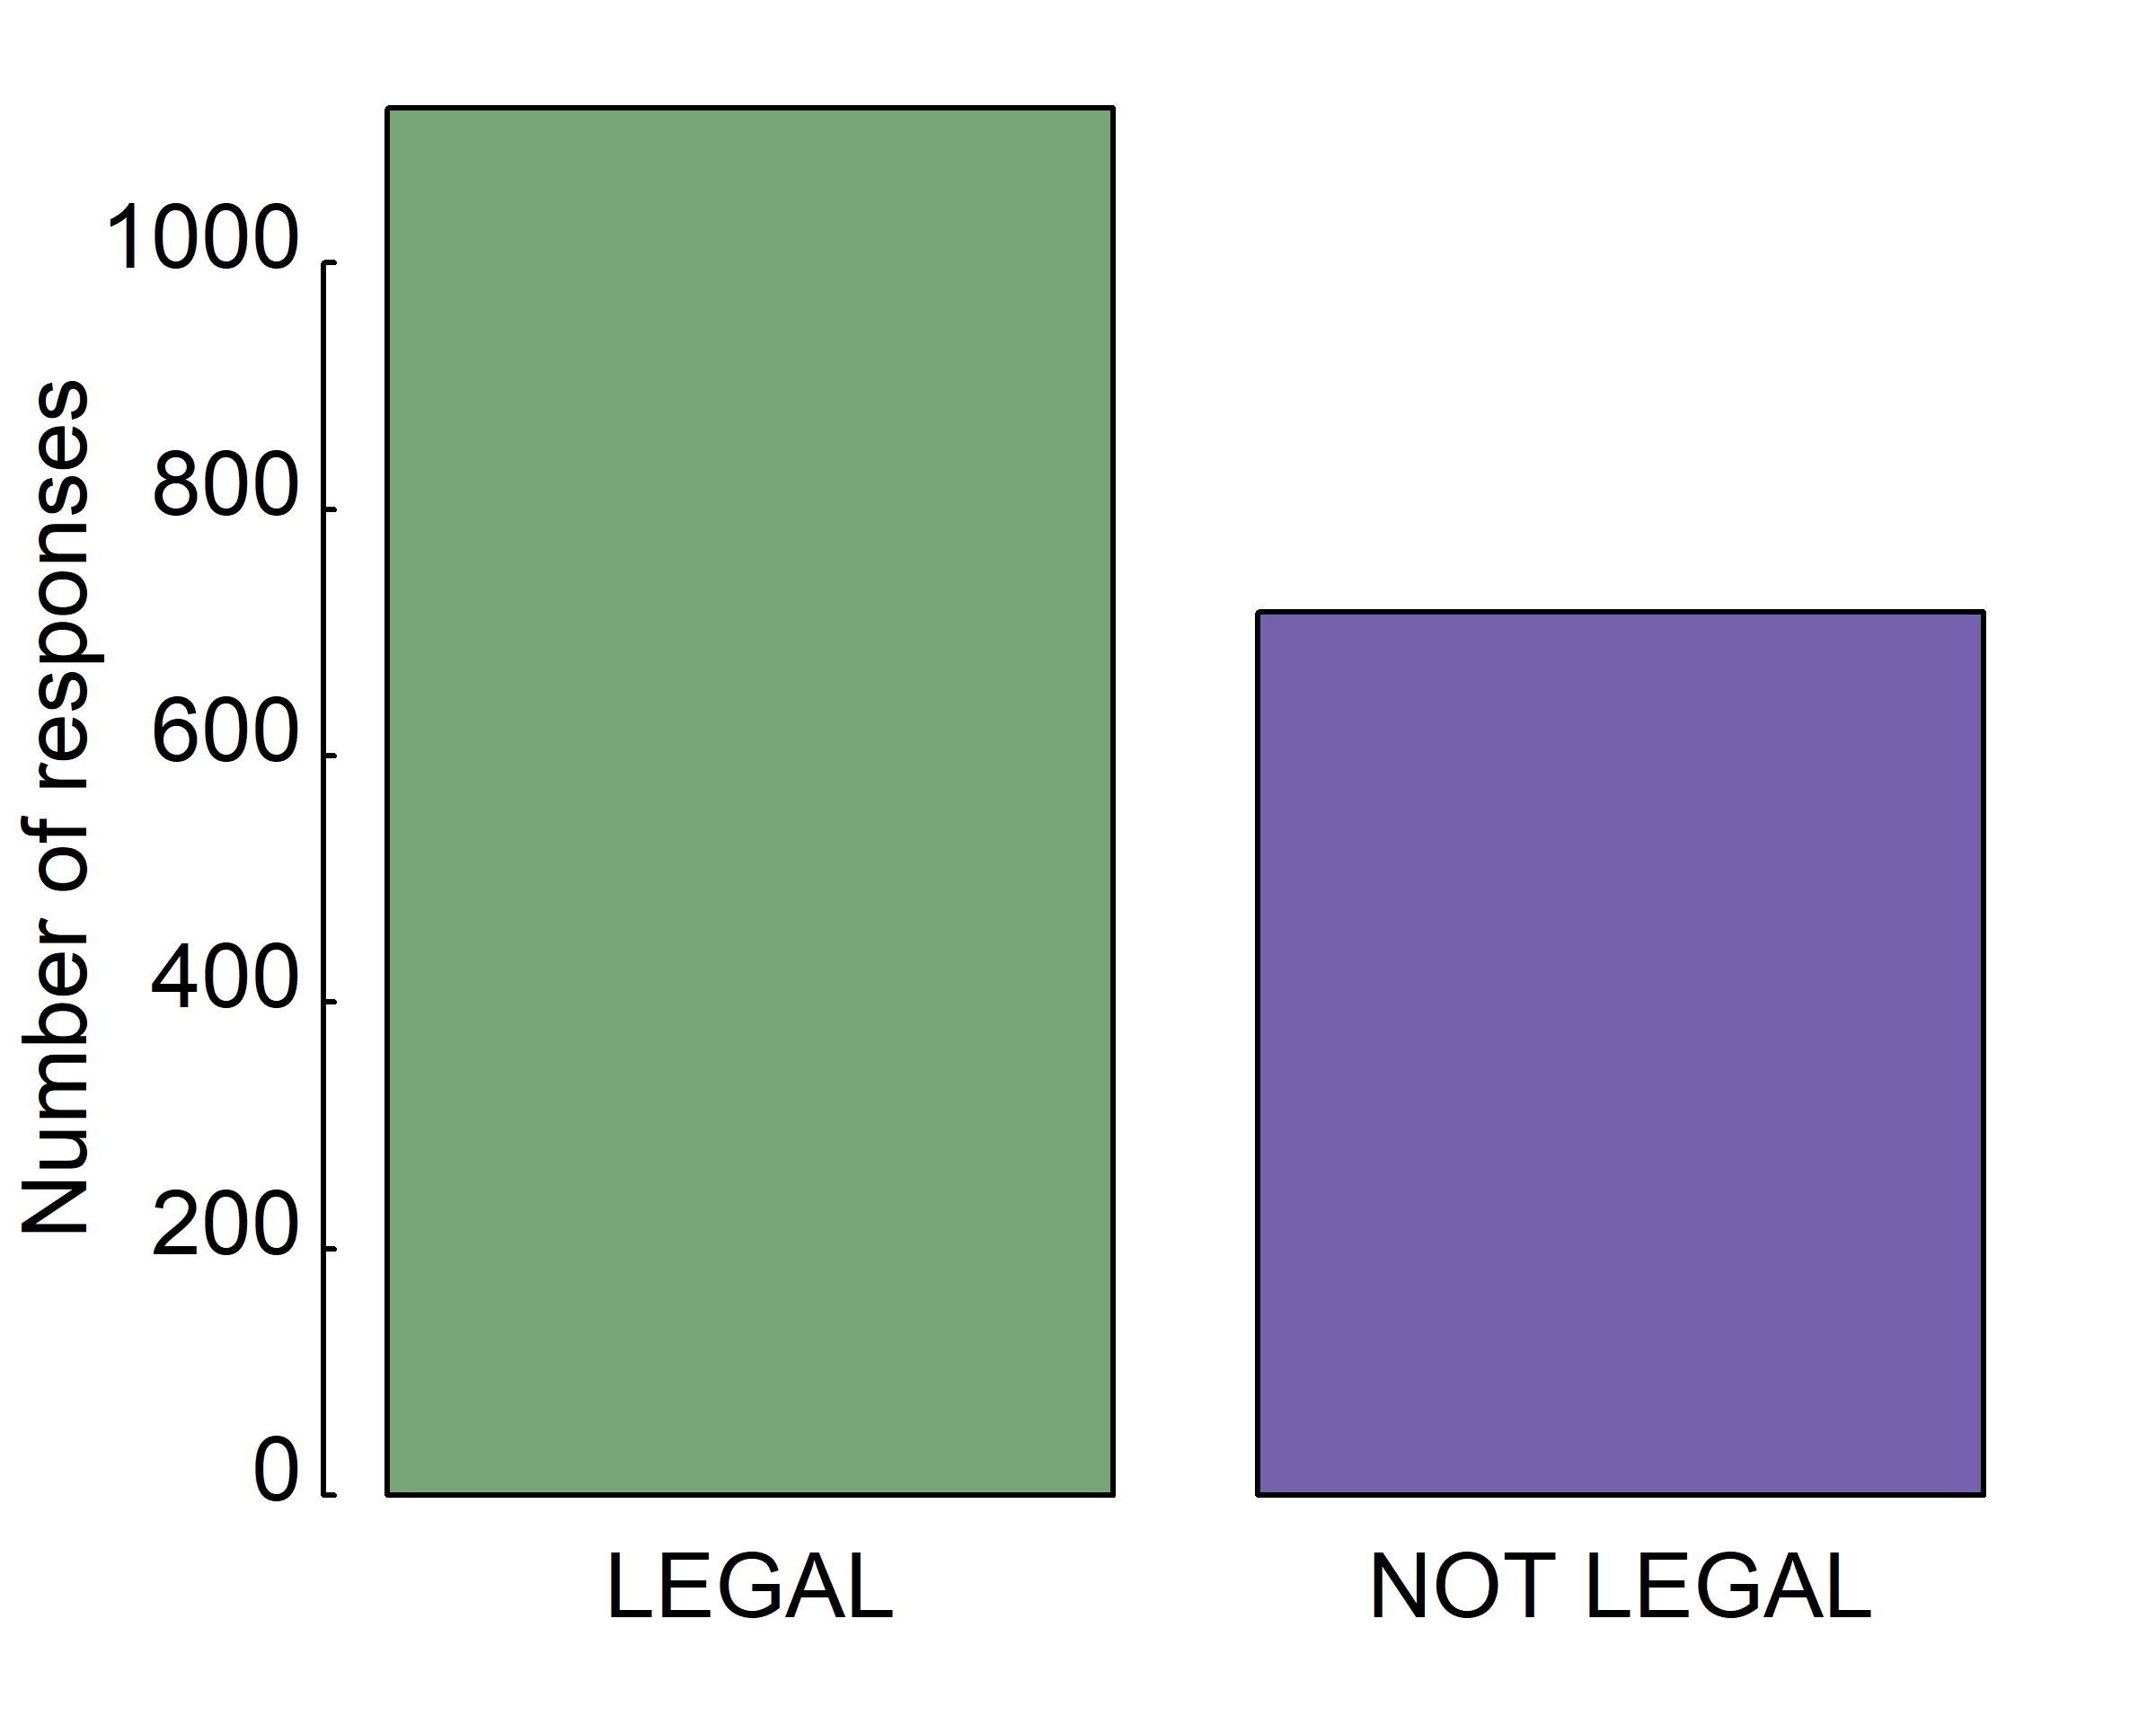
\includegraphics[width=0.5\linewidth]{03_Getting_started_with_a_data_analaysis_files/figure-latex/unnamed-chunk-44-5} 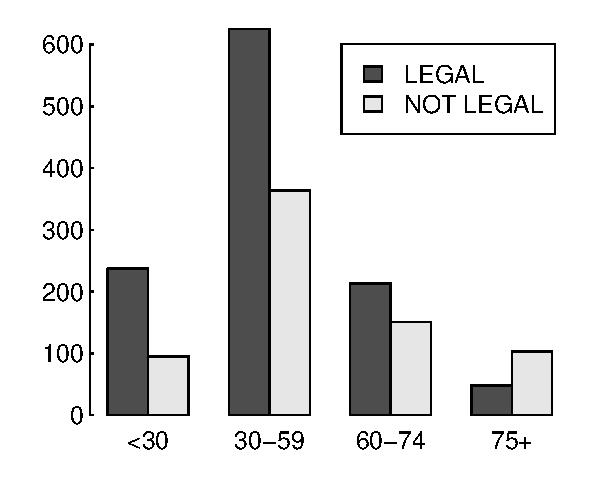
\includegraphics[width=0.5\linewidth]{03_Getting_started_with_a_data_analaysis_files/figure-latex/unnamed-chunk-44-6} \end{figure}

\hypertarget{histogram}{%
\subsubsection{Histogram}\label{histogram}}

Histograms display the distribution of a continuous variable by dividing the range of scores into a specified number of bins on the x-axis and displaying the frequency of scores in each bin on the y-axis. You can create histograms with the function

\begin{Shaded}
\begin{Highlighting}[]
\FunctionTok{par}\NormalTok{(}\AttributeTok{mar =} \FunctionTok{c}\NormalTok{(}\DecValTok{2}\NormalTok{, }\DecValTok{2}\NormalTok{, }\DecValTok{2}\NormalTok{, }\FloatTok{0.1}\NormalTok{), }\AttributeTok{las=}\DecValTok{1}\NormalTok{, }\AttributeTok{mgp=}\FunctionTok{c}\NormalTok{(}\FloatTok{2.5}\NormalTok{,}\FloatTok{0.1}\NormalTok{, }\DecValTok{0}\NormalTok{), }\AttributeTok{tcl=}\FloatTok{0.15}\NormalTok{)}
\FunctionTok{hist}\NormalTok{(survey}\SpecialCharTok{$}\NormalTok{Wr.Hnd)}
\end{Highlighting}
\end{Shaded}

\begin{center}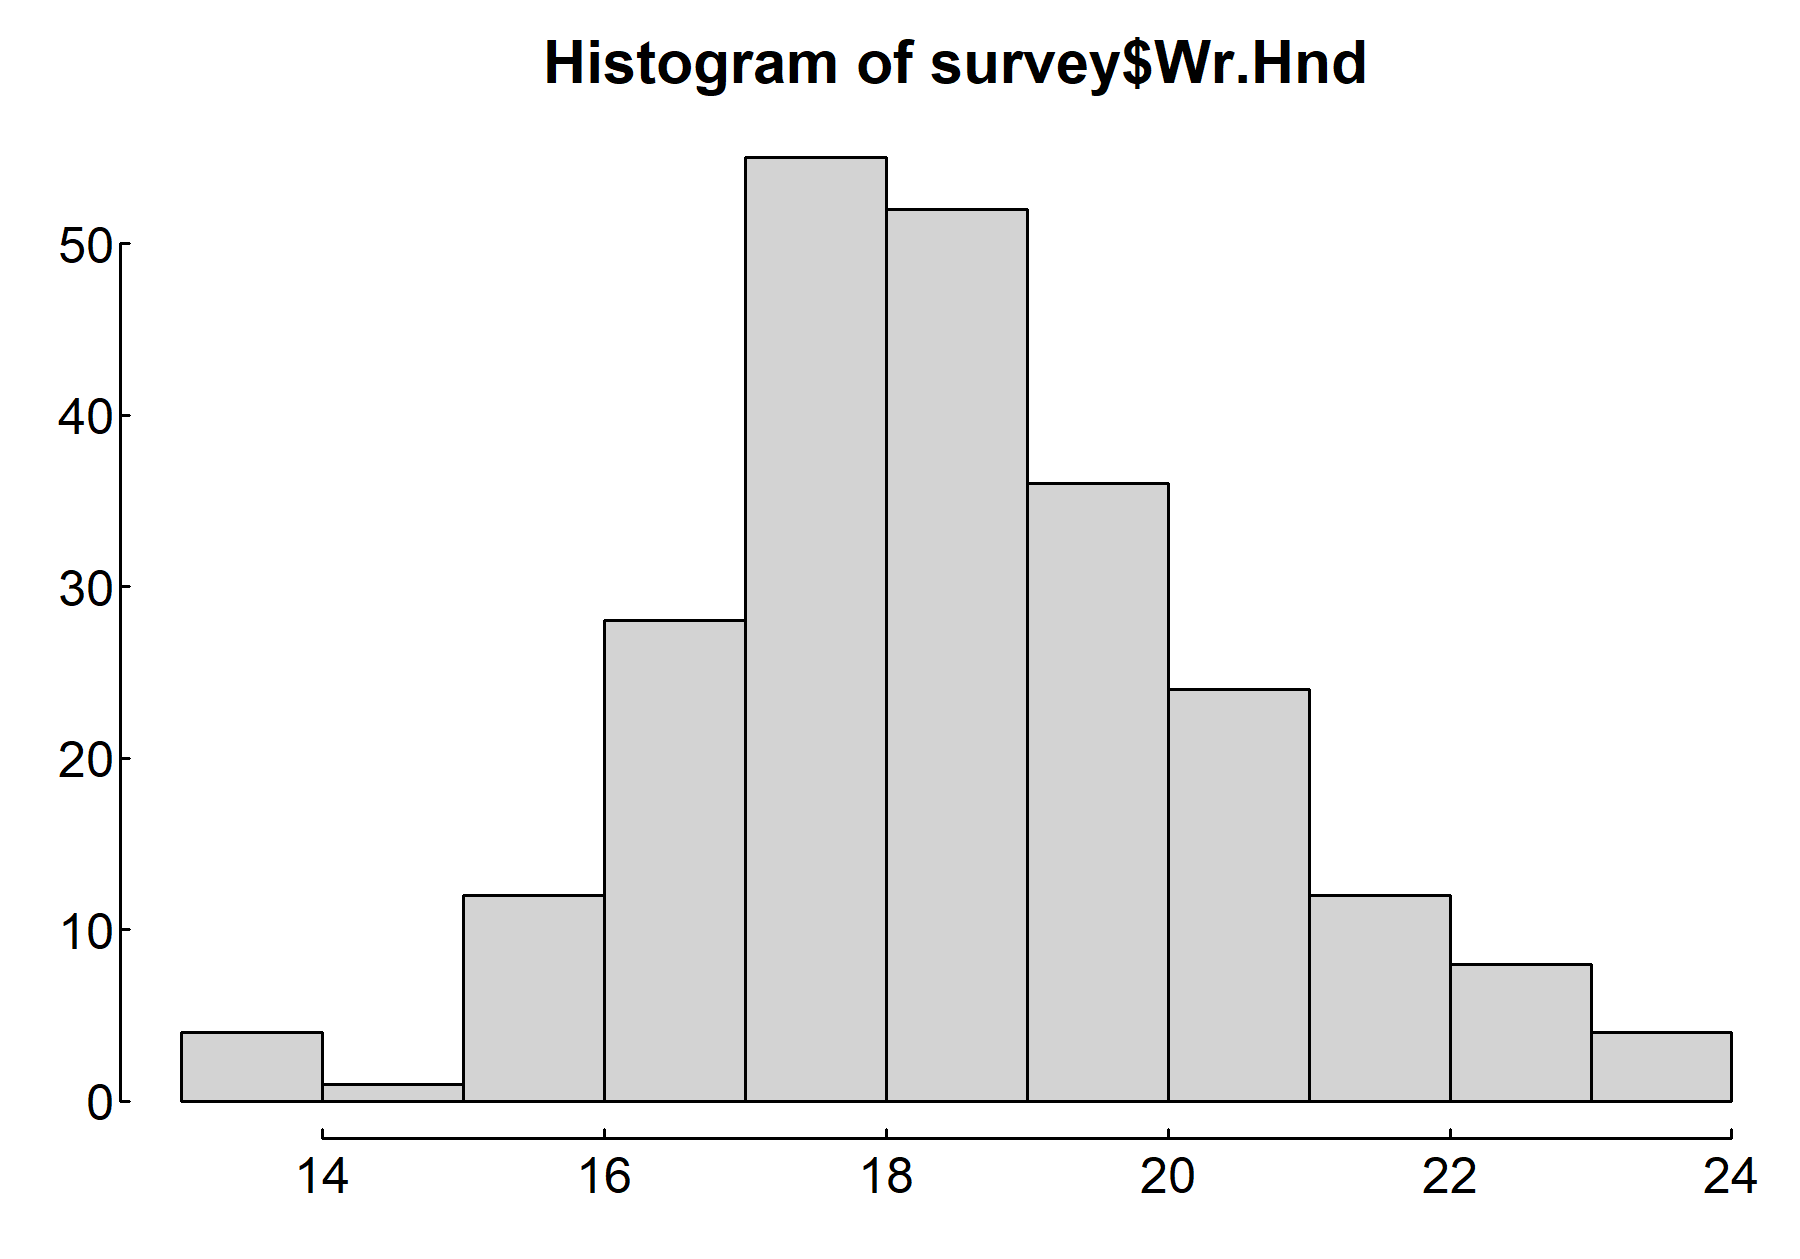
\includegraphics[width=0.6\linewidth]{03_Getting_started_with_a_data_analaysis_files/figure-latex/unnamed-chunk-45-1} \end{center}

where \texttt{survey\$Wr.Hnd} is a numeric vector of values. The option \texttt{freq=FALSE} creates a plot based on probability densities rather than frequencies. The \texttt{breaks=} option controls the number of bins. The default produces equally spaced breaks when defining the cells of the histogram. The following listing provides the code for four variations of a histogram; the results are plotted in figure 6.8.

\begin{Shaded}
\begin{Highlighting}[]
\FunctionTok{par}\NormalTok{(}\AttributeTok{mar =} \FunctionTok{c}\NormalTok{(}\DecValTok{4}\NormalTok{, }\DecValTok{4}\NormalTok{, }\DecValTok{2}\NormalTok{, }\FloatTok{0.1}\NormalTok{), }\AttributeTok{las=}\DecValTok{1}\NormalTok{, }\AttributeTok{mgp=}\FunctionTok{c}\NormalTok{(}\FloatTok{2.5}\NormalTok{,}\FloatTok{0.1}\NormalTok{, }\DecValTok{0}\NormalTok{), }\AttributeTok{tcl=}\FloatTok{0.15}\NormalTok{)}
\FunctionTok{hist}\NormalTok{(survey}\SpecialCharTok{$}\NormalTok{Wr.Hnd)}
\FunctionTok{hist}\NormalTok{(survey}\SpecialCharTok{$}\NormalTok{Wr.Hnd,}
     \AttributeTok{breaks=}\DecValTok{20}\NormalTok{, }\AttributeTok{col =} \StringTok{"lightblue"}\NormalTok{)}
\FunctionTok{hist}\NormalTok{(survey}\SpecialCharTok{$}\NormalTok{Wr.Hnd,}
     \AttributeTok{breaks=}\DecValTok{20}\NormalTok{, }\AttributeTok{col =} \StringTok{"lightblue"}\NormalTok{,}
     \AttributeTok{freq =}\NormalTok{ F)}
\FunctionTok{rug}\NormalTok{(}\FunctionTok{jitter}\NormalTok{(survey}\SpecialCharTok{$}\NormalTok{Wr.Hnd))}
\FunctionTok{lines}\NormalTok{(}\FunctionTok{density}\NormalTok{(survey}\SpecialCharTok{$}\NormalTok{Wr.Hnd, }\AttributeTok{na.rm =} \ConstantTok{TRUE}\NormalTok{), }
      \AttributeTok{col=}\StringTok{"red"}\NormalTok{, }\AttributeTok{lwd=}\DecValTok{2}\NormalTok{)}
\FunctionTok{range}\NormalTok{(survey}\SpecialCharTok{$}\NormalTok{Wr.Hnd, }\AttributeTok{na.rm =}\NormalTok{ T)}
\CommentTok{\#\textgreater{} [1] 13.0 23.2}
\FunctionTok{hist}\NormalTok{(survey}\SpecialCharTok{$}\NormalTok{Wr.Hnd,}
     \AttributeTok{breaks=}\FunctionTok{seq}\NormalTok{(}\AttributeTok{from=}\DecValTok{13}\NormalTok{, }\AttributeTok{to=}\DecValTok{24}\NormalTok{, }\AttributeTok{by=}\DecValTok{1}\NormalTok{), }
     \AttributeTok{col =} \StringTok{"lightblue"}\NormalTok{, }\AttributeTok{freq =}\NormalTok{ F)}
\FunctionTok{curve}\NormalTok{(}\FunctionTok{dnorm}\NormalTok{(x, }\AttributeTok{mean=}\FunctionTok{mean}\NormalTok{(survey}\SpecialCharTok{$}\NormalTok{Wr.Hnd, }\AttributeTok{na.rm =}\NormalTok{ T), }
            \AttributeTok{sd=}\FunctionTok{sd}\NormalTok{(survey}\SpecialCharTok{$}\NormalTok{Wr.Hnd, }\AttributeTok{na.rm =}\NormalTok{ T)), }
      \AttributeTok{from=}\DecValTok{13}\NormalTok{, }\AttributeTok{to=}\DecValTok{24}\NormalTok{, }\AttributeTok{add=}\NormalTok{T, }\AttributeTok{col=}\StringTok{"red"}\NormalTok{, }\AttributeTok{lwd=}\DecValTok{2}\NormalTok{)}
\end{Highlighting}
\end{Shaded}

\begin{figure}
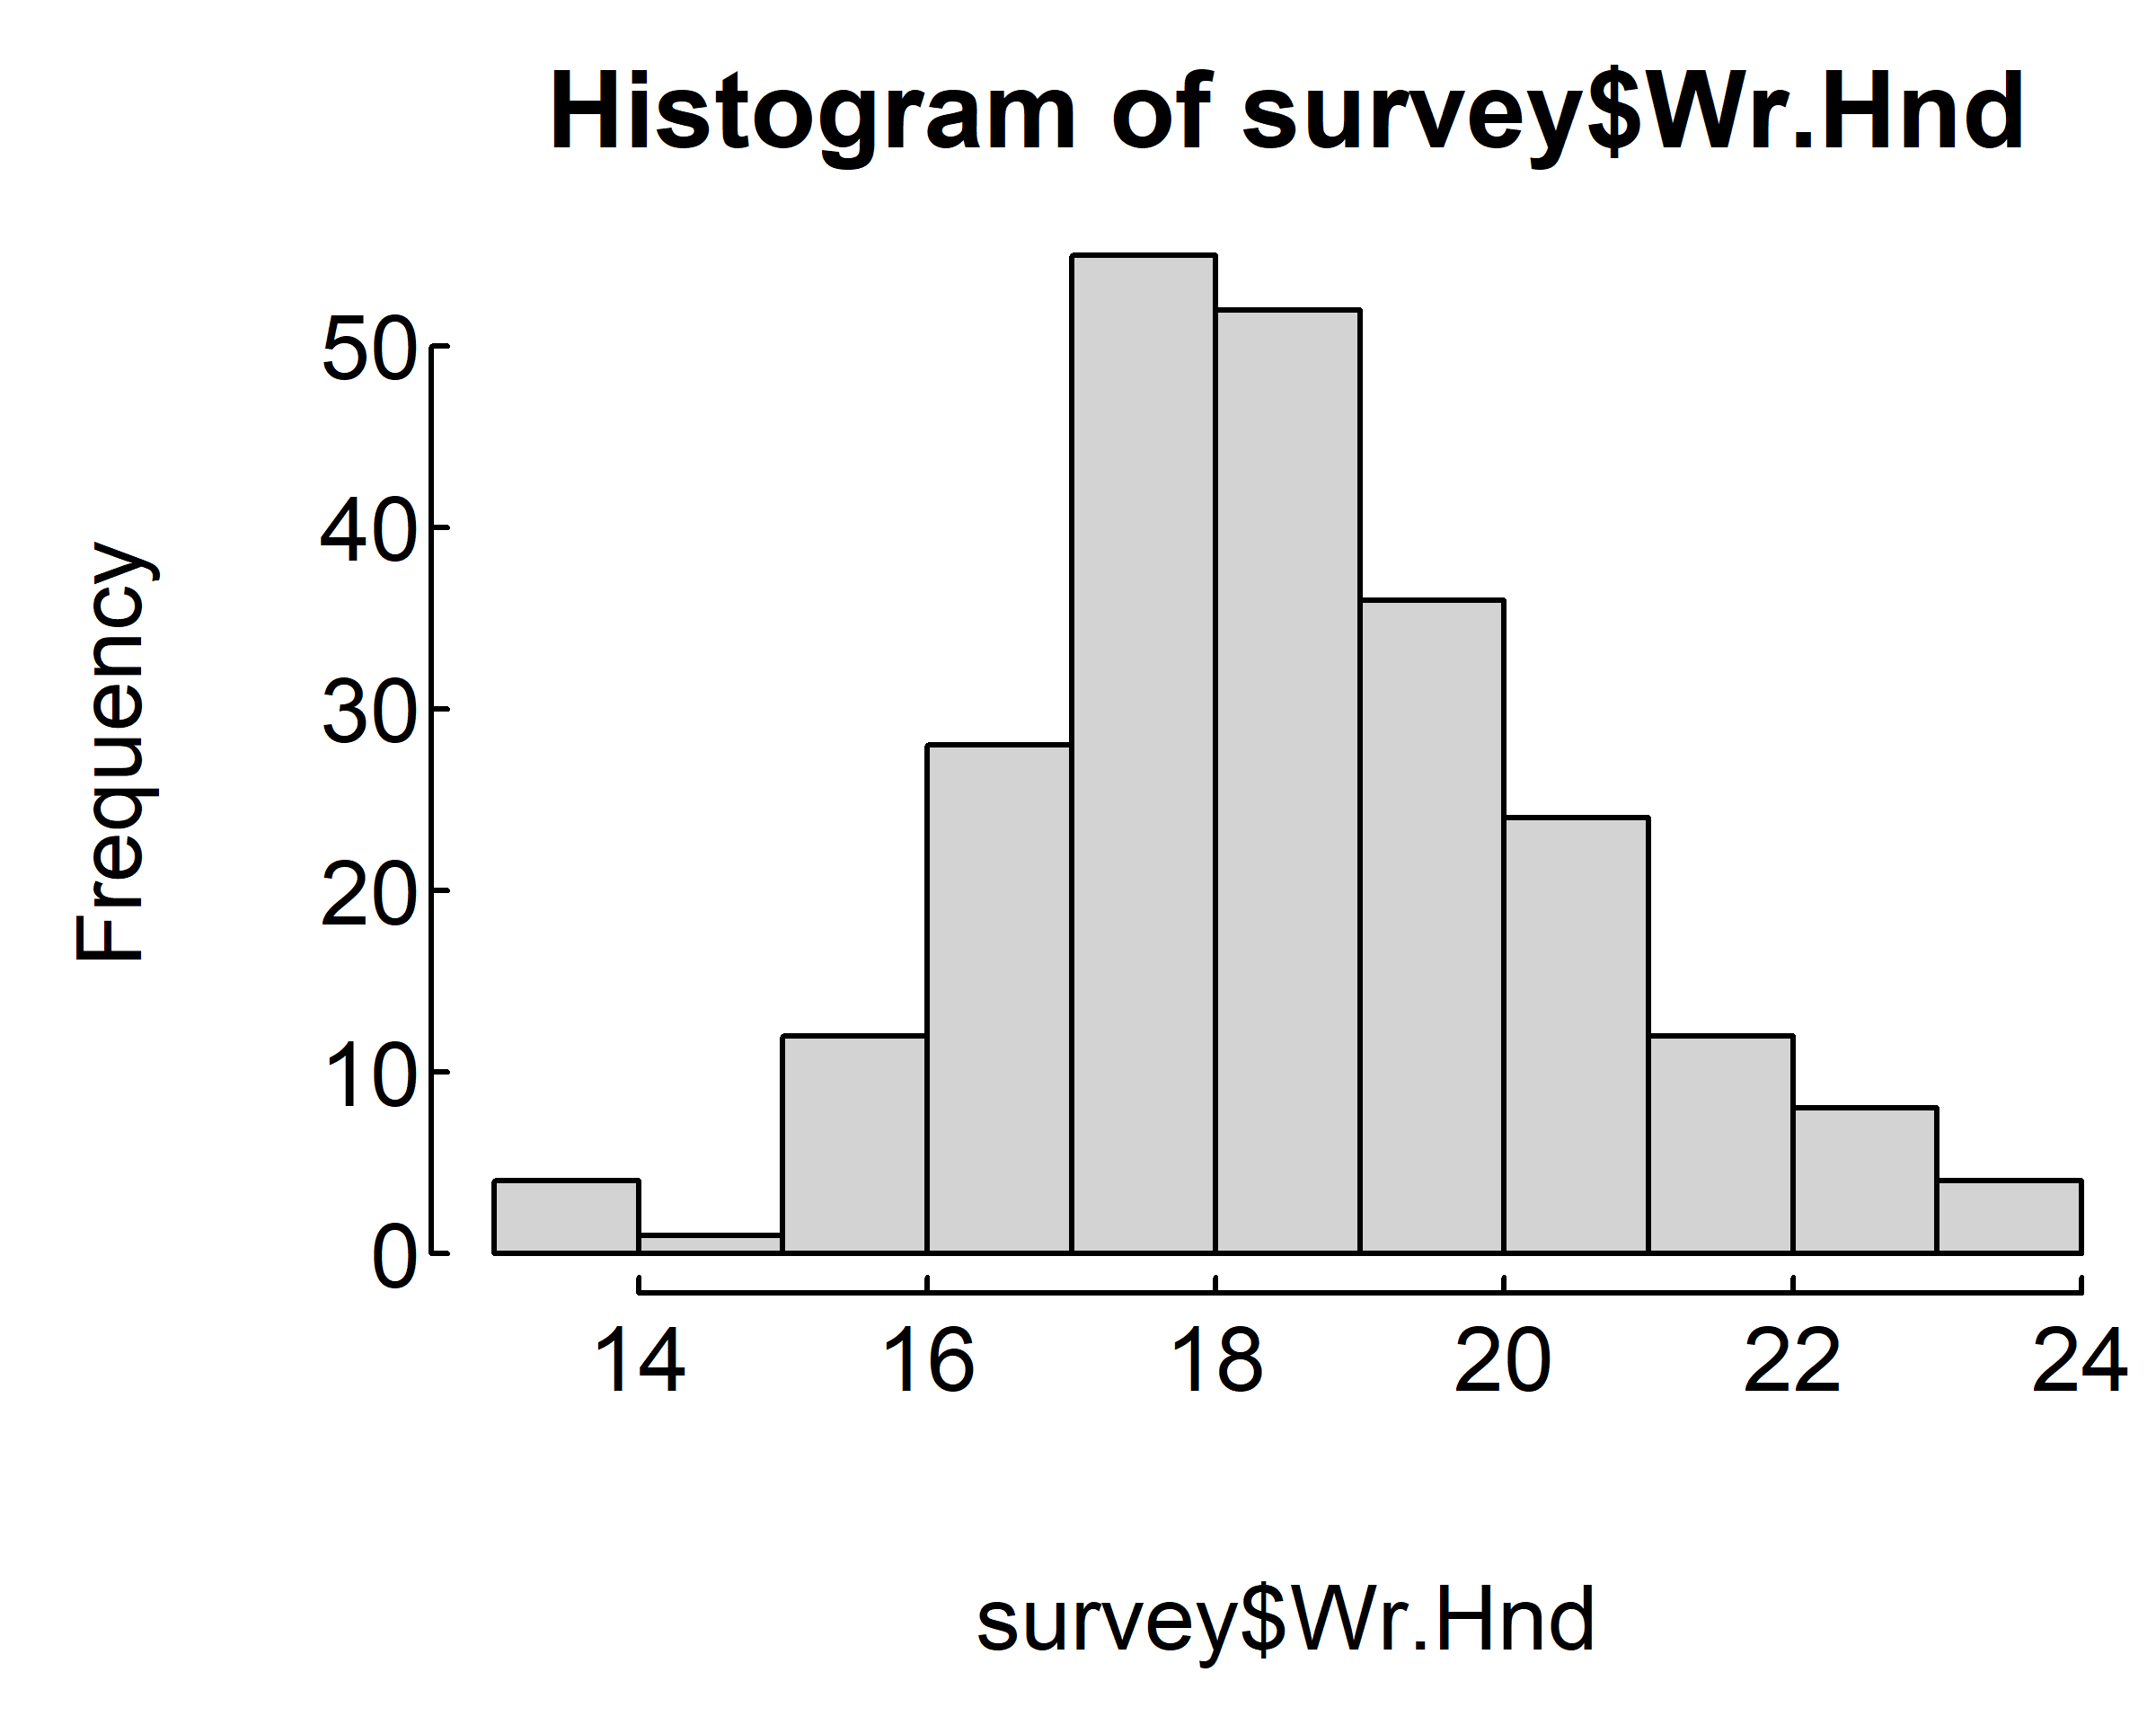
\includegraphics[width=0.5\linewidth]{03_Getting_started_with_a_data_analaysis_files/figure-latex/unnamed-chunk-46-1} 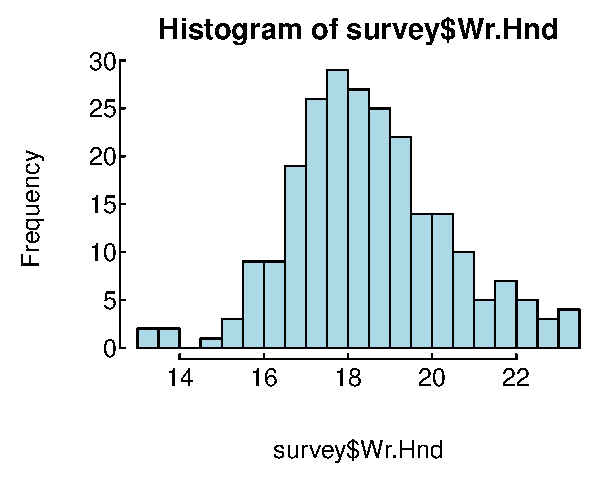
\includegraphics[width=0.5\linewidth]{03_Getting_started_with_a_data_analaysis_files/figure-latex/unnamed-chunk-46-2} 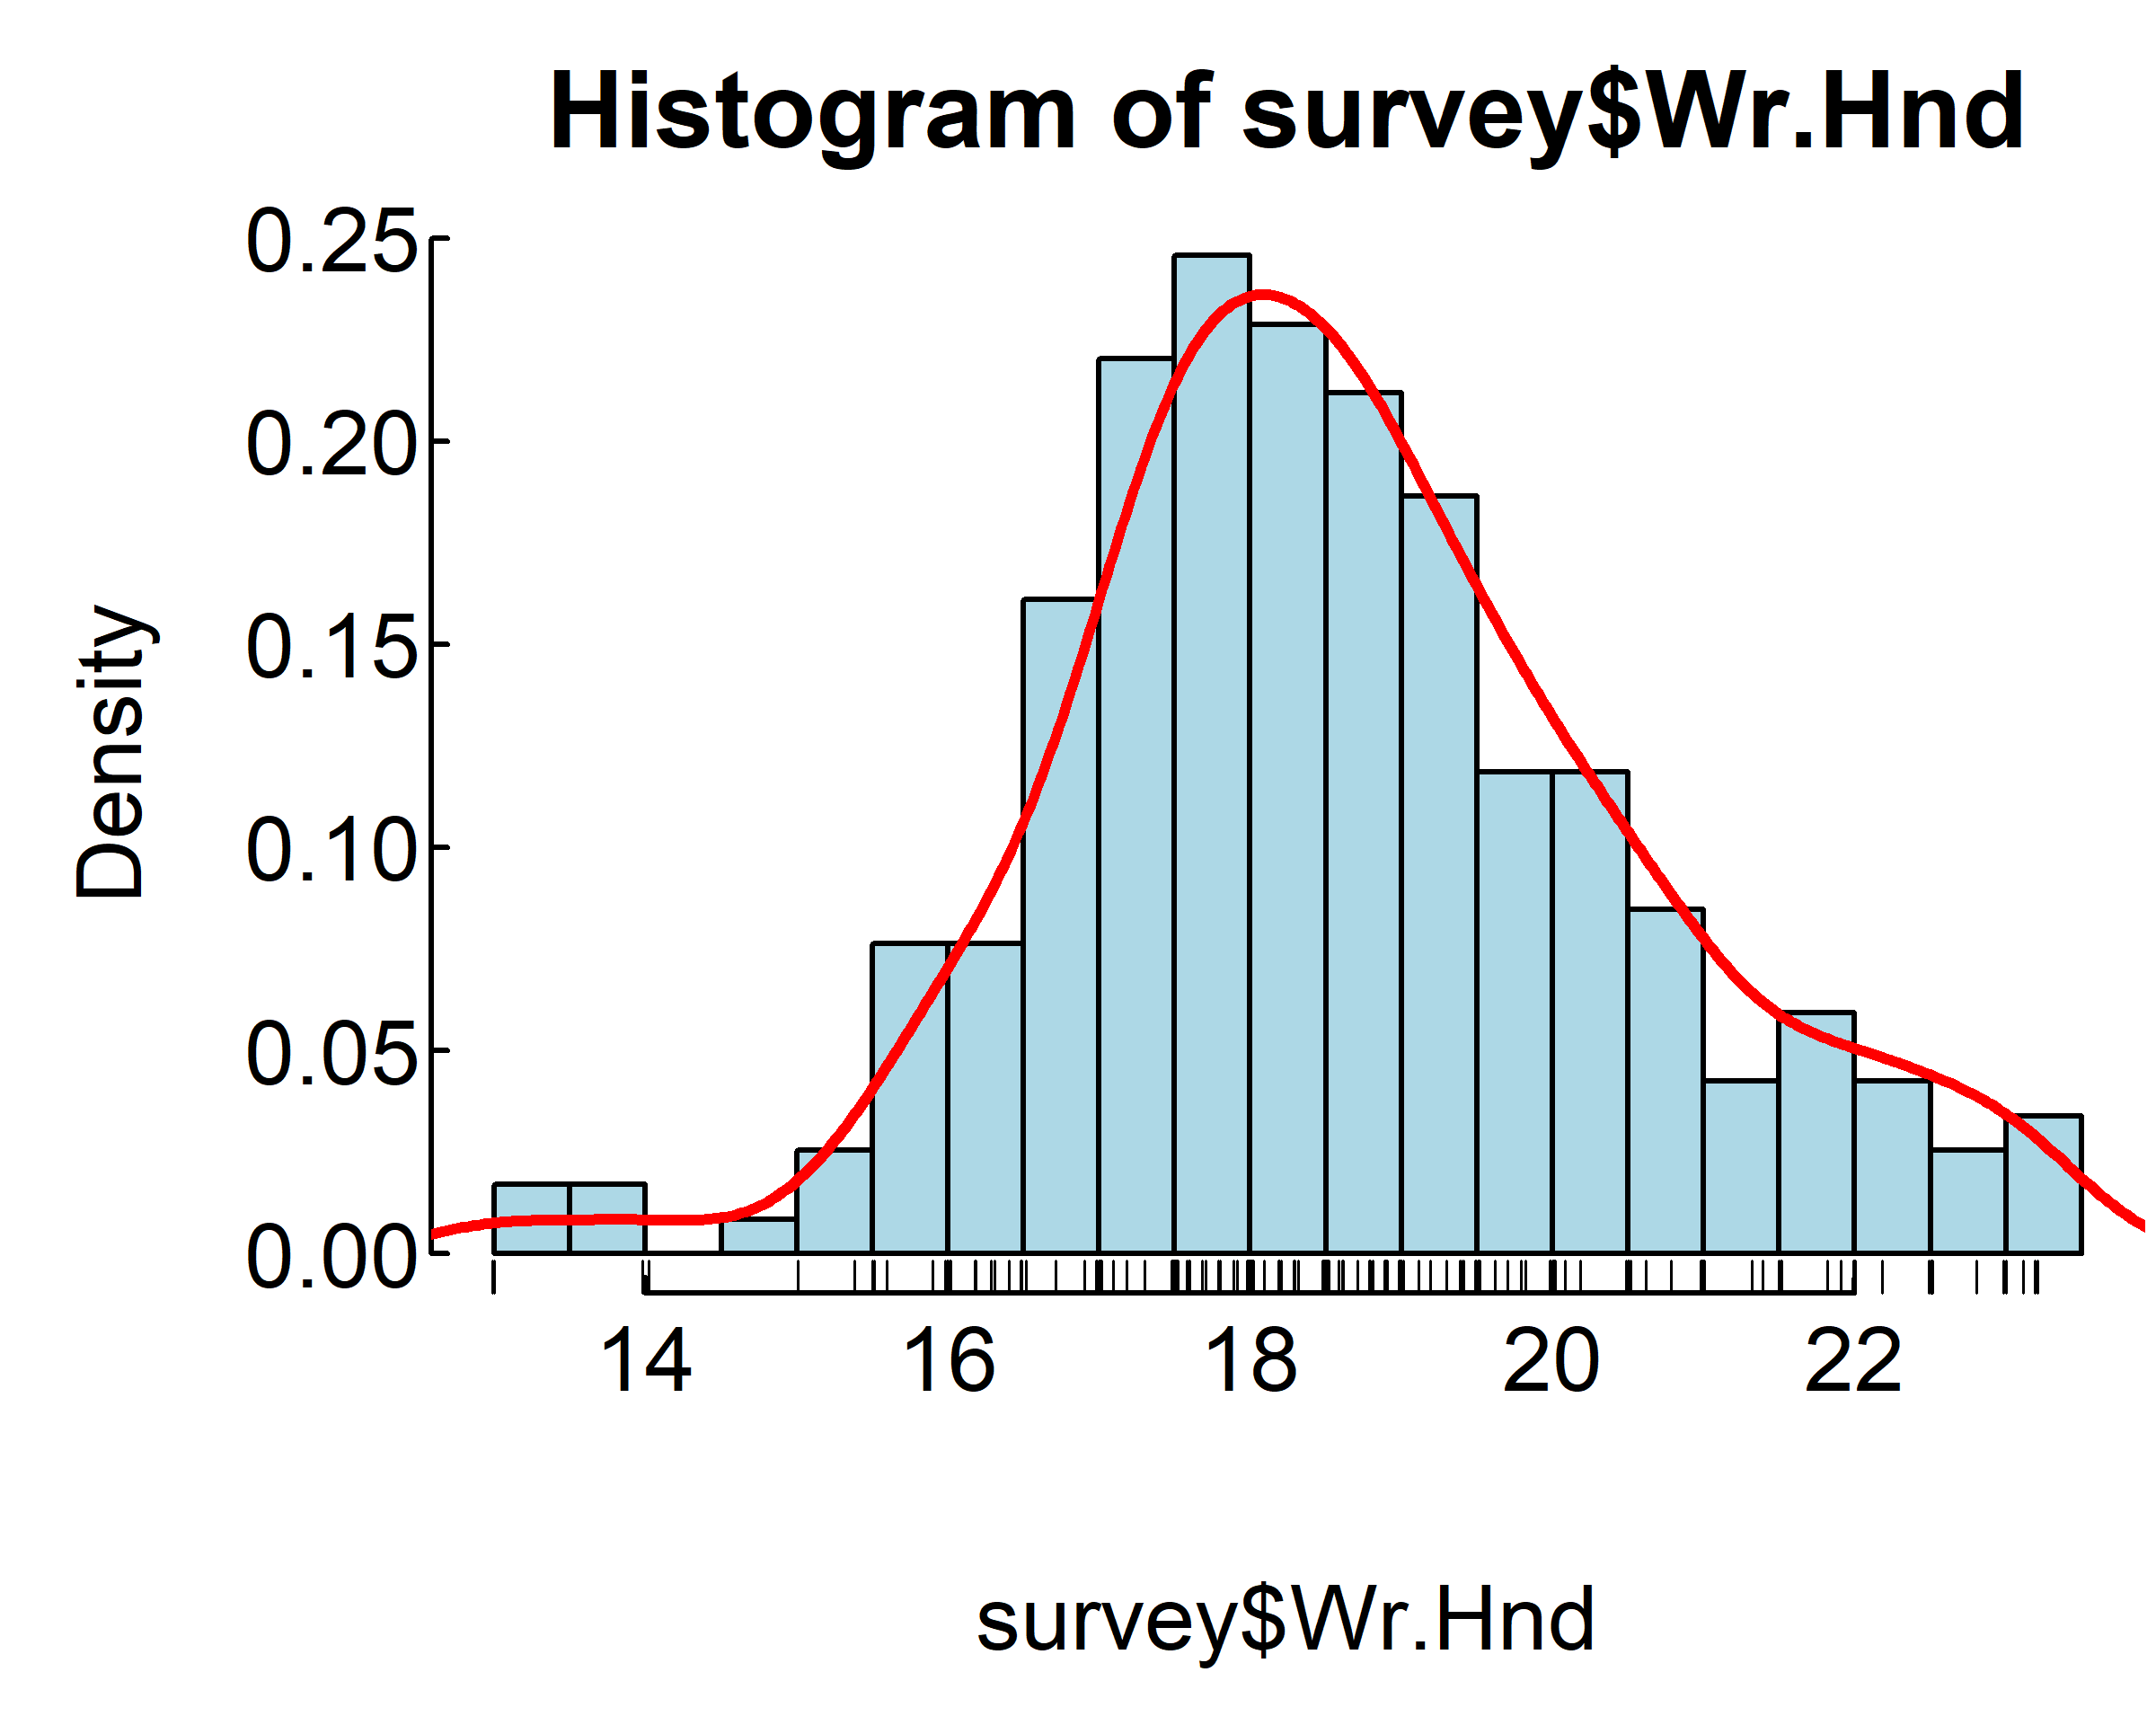
\includegraphics[width=0.5\linewidth]{03_Getting_started_with_a_data_analaysis_files/figure-latex/unnamed-chunk-46-3} 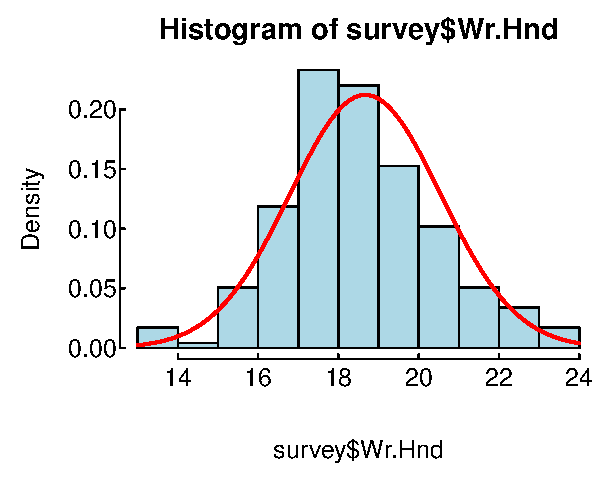
\includegraphics[width=0.5\linewidth]{03_Getting_started_with_a_data_analaysis_files/figure-latex/unnamed-chunk-46-4} \end{figure}

\hypertarget{box-plot}{%
\subsubsection{Box plot}\label{box-plot}}

A box-and-whiskers plot describes the distribution of a continuous variable by plotting its five-number summary: the minimum, lower quartile (25th percentile), median (50th percentile), upper quartile (75th percentile), and maximum. It can also display observations that may be outliers (values outside the range of \(\pm1.5*IQR\), where IQR is the interquartile range defined as the upper quartile minus the lower quartile). For example, this statement produces the plot shown below:

\begin{Shaded}
\begin{Highlighting}[]
\FunctionTok{par}\NormalTok{(}\AttributeTok{mar =} \FunctionTok{c}\NormalTok{(}\DecValTok{2}\NormalTok{, }\DecValTok{2}\NormalTok{, }\DecValTok{2}\NormalTok{, }\FloatTok{0.1}\NormalTok{), }\AttributeTok{las=}\DecValTok{1}\NormalTok{, }\AttributeTok{mgp=}\FunctionTok{c}\NormalTok{(}\FloatTok{2.5}\NormalTok{,}\FloatTok{0.1}\NormalTok{, }\DecValTok{0}\NormalTok{), }\AttributeTok{tcl=}\FloatTok{0.15}\NormalTok{)}
\FunctionTok{boxplot}\NormalTok{(survey}\SpecialCharTok{$}\NormalTok{Wr.Hnd, }\AttributeTok{main=}\StringTok{"Box plot"}\NormalTok{, }\AttributeTok{ylab=}\StringTok{"cm"}\NormalTok{)}
\end{Highlighting}
\end{Shaded}

\begin{center}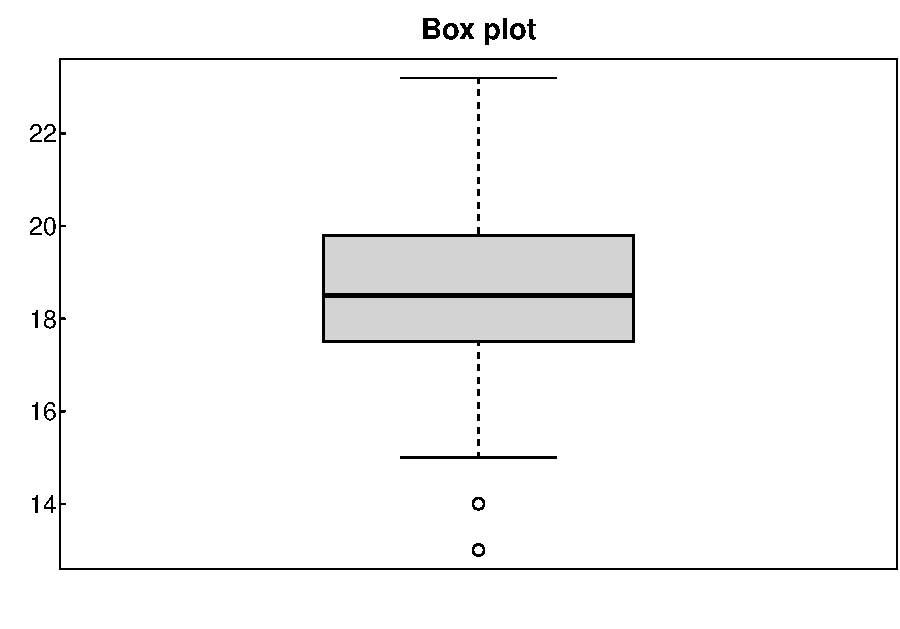
\includegraphics[width=0.6\linewidth]{03_Getting_started_with_a_data_analaysis_files/figure-latex/unnamed-chunk-47-1} \end{center}

Box plots can be created for individual variables or for variables by group. The format is

\begin{Shaded}
\begin{Highlighting}[]
\FunctionTok{boxplot}\NormalTok{(formula, }\AttributeTok{data=}\NormalTok{dataframe)}
\end{Highlighting}
\end{Shaded}

where \texttt{formula} is a formula and \texttt{dataframe} denotes the data frame (or list) providing the data. An example of a formula is \texttt{y\ \textasciitilde{}\ A}, where a separate box plot for numeric variable \texttt{y} is generated for each value of categorical variable \texttt{A}. The formula \texttt{y\ \textasciitilde{}\ A*B} would produce a box plot of numeric variable \texttt{y}, for each combination of levels in categorical variables \texttt{A} and \texttt{B}.

Adding the option \texttt{horizontal=TRUE} to reverse the axis orientation.

The following code revisits the impact of sex on height with parallel box plots.

\begin{Shaded}
\begin{Highlighting}[]
\FunctionTok{par}\NormalTok{(}\AttributeTok{mar =} \FunctionTok{c}\NormalTok{(}\DecValTok{4}\NormalTok{, }\DecValTok{4}\NormalTok{, }\DecValTok{2}\NormalTok{, }\FloatTok{0.1}\NormalTok{), }\AttributeTok{las=}\DecValTok{1}\NormalTok{, }\AttributeTok{mgp=}\FunctionTok{c}\NormalTok{(}\FloatTok{2.5}\NormalTok{,}\FloatTok{0.1}\NormalTok{, }\DecValTok{0}\NormalTok{), }\AttributeTok{tcl=}\FloatTok{0.15}\NormalTok{)}
\FunctionTok{boxplot}\NormalTok{(Height }\SpecialCharTok{\textasciitilde{}}\NormalTok{ Sex, }\AttributeTok{data=}\NormalTok{survey)}
\FunctionTok{boxplot}\NormalTok{(Height }\SpecialCharTok{\textasciitilde{}}\NormalTok{ Sex, }\AttributeTok{data=}\NormalTok{survey, }\AttributeTok{horizontal=}\ConstantTok{TRUE}\NormalTok{)}
\end{Highlighting}
\end{Shaded}

\begin{figure}
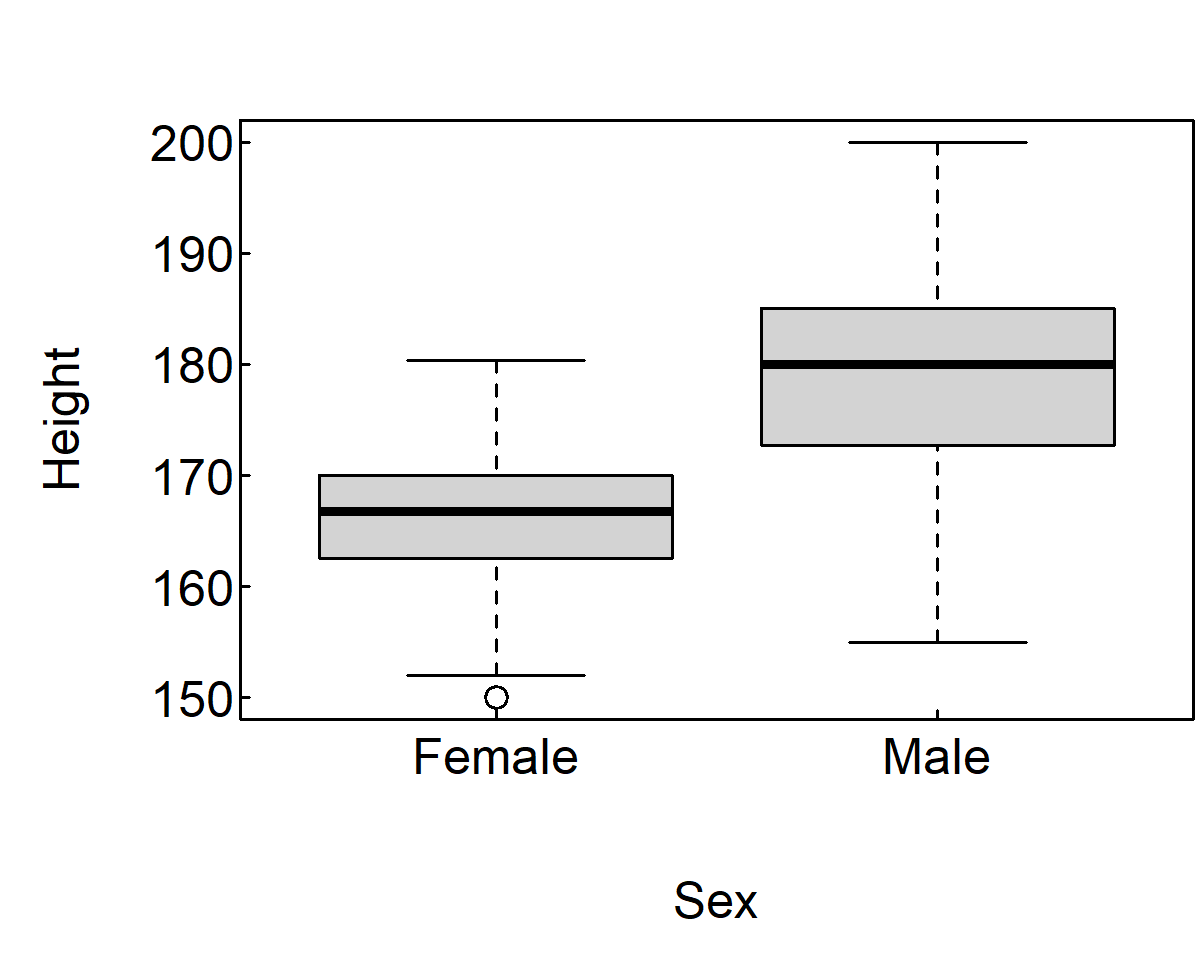
\includegraphics[width=0.5\linewidth]{03_Getting_started_with_a_data_analaysis_files/figure-latex/unnamed-chunk-49-1} 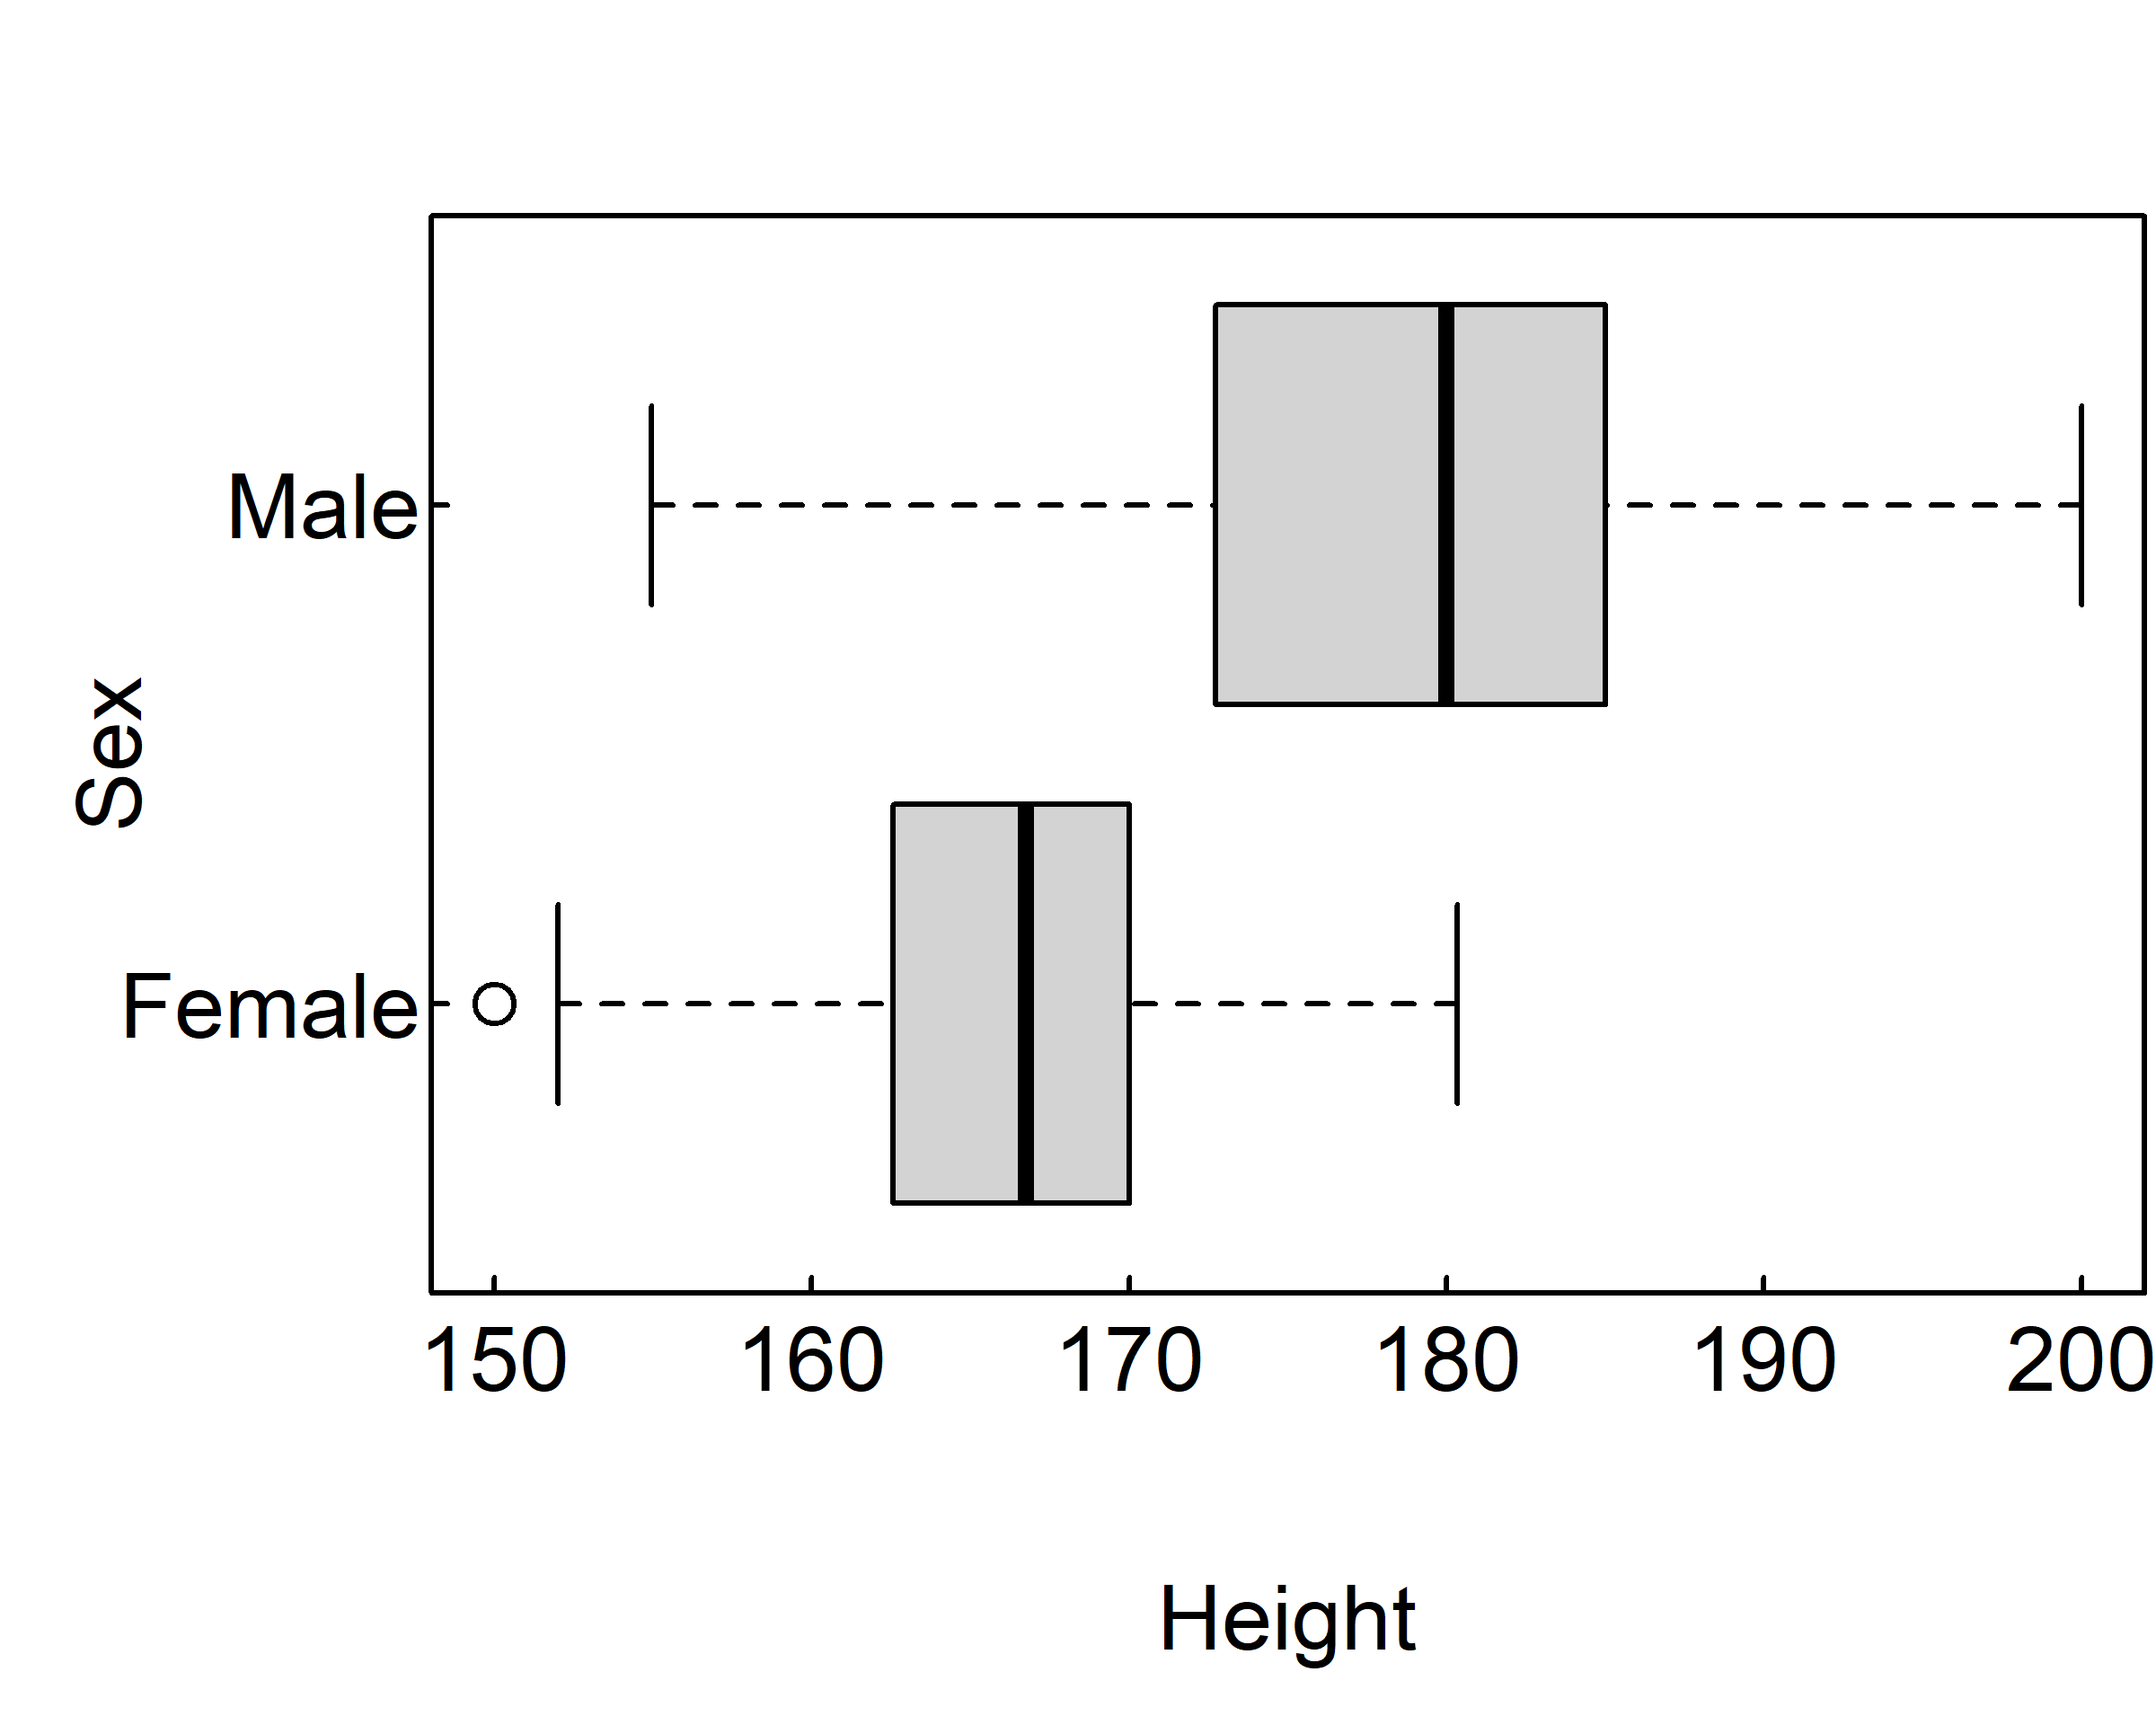
\includegraphics[width=0.5\linewidth]{03_Getting_started_with_a_data_analaysis_files/figure-latex/unnamed-chunk-49-2} \end{figure}

\hypertarget{scatterplot}{%
\subsubsection{Scatterplot}\label{scatterplot}}

To create a scatterplot, you use the \texttt{plot()} function. A scatterplot creates points (or sometimes bubbles or other symbols) on your chart. Each point corresponds to an observation in your data. You've probably seen or created this type of graphic a million times, so you already know that scatterplots use the Cartesian coordinate system, where one variable is mapped to the x‐axis and a second variable is mapped to the y‐axis.

The most common high level function used to produce plots in R is the \texttt{plot()} function.

\begin{Shaded}
\begin{Highlighting}[]
\FunctionTok{par}\NormalTok{(}\AttributeTok{mar =} \FunctionTok{c}\NormalTok{(}\DecValTok{3}\NormalTok{, }\DecValTok{3}\NormalTok{, }\DecValTok{2}\NormalTok{, }\FloatTok{0.1}\NormalTok{), }\AttributeTok{las=}\DecValTok{1}\NormalTok{, }\AttributeTok{mgp=}\FunctionTok{c}\NormalTok{(}\FloatTok{1.5}\NormalTok{,}\FloatTok{0.1}\NormalTok{, }\DecValTok{0}\NormalTok{), }\AttributeTok{tcl=}\FloatTok{0.15}\NormalTok{)}
\FunctionTok{plot}\NormalTok{(survey}\SpecialCharTok{$}\NormalTok{Wr.Hnd)}
\end{Highlighting}
\end{Shaded}

\begin{center}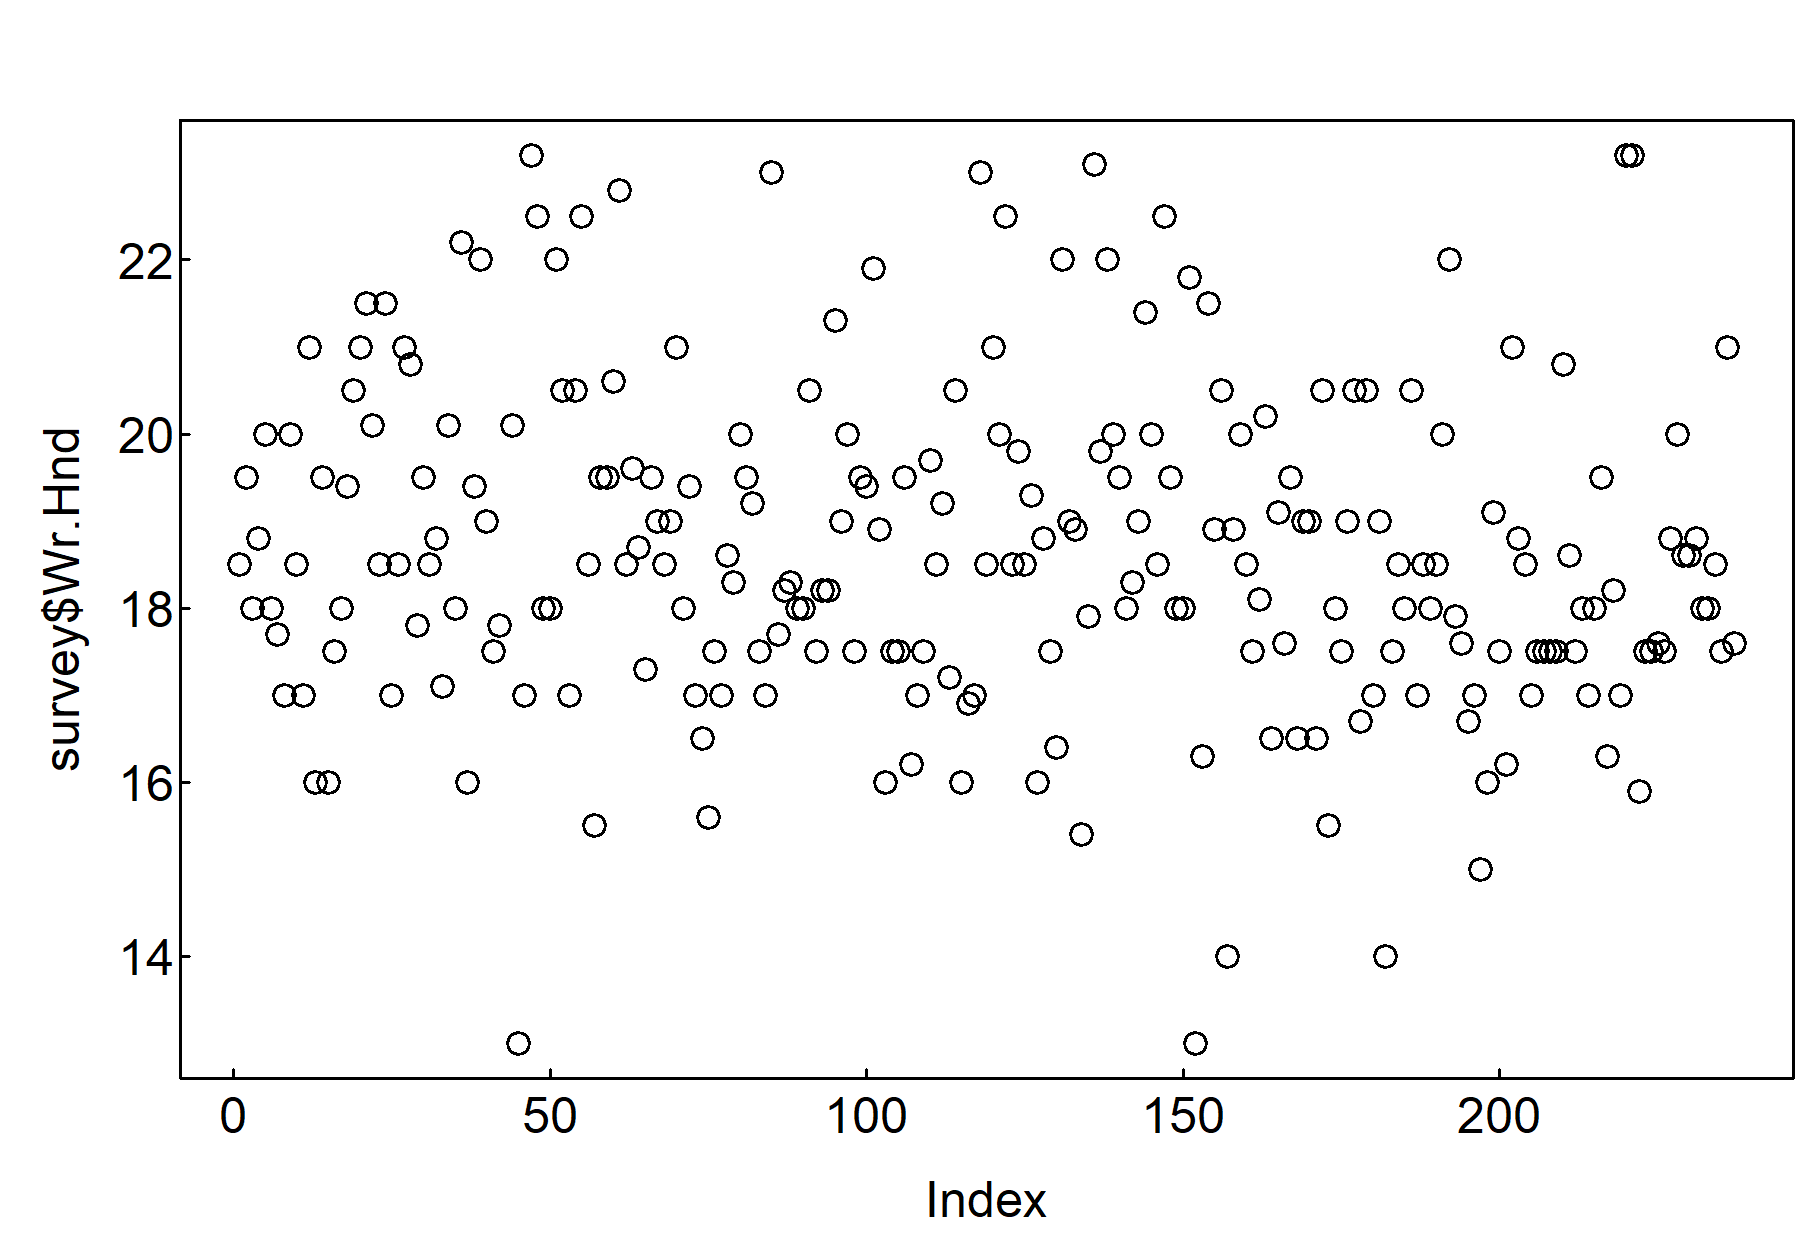
\includegraphics[width=0.6\linewidth]{03_Getting_started_with_a_data_analaysis_files/figure-latex/unnamed-chunk-50-1} \end{center}

R has plotted the values of \texttt{Wr.Hnd} (on the y axis) against an index since we are only plotting one variable to plot. The index is just the order of the \texttt{Wr.Hnd} values in the data frame (1 first in the data frame and 237 last). The \texttt{Wr.Hnd} variable name has been automatically included as a y axis label and the axes scales have been automatically set.

To plot a scatterplot of one numeric variable against another numeric variable we just need to include both variables as arguments when using the \texttt{plot()} function. For example to plot \texttt{Wr.Hnd} on the y axis and \texttt{Height} of the x axis.

\begin{Shaded}
\begin{Highlighting}[]
\FunctionTok{par}\NormalTok{(}\AttributeTok{mar =} \FunctionTok{c}\NormalTok{(}\DecValTok{3}\NormalTok{, }\DecValTok{3}\NormalTok{, }\DecValTok{2}\NormalTok{, }\FloatTok{0.1}\NormalTok{), }\AttributeTok{las=}\DecValTok{1}\NormalTok{, }\AttributeTok{mgp=}\FunctionTok{c}\NormalTok{(}\FloatTok{1.5}\NormalTok{,}\FloatTok{0.1}\NormalTok{, }\DecValTok{0}\NormalTok{), }\AttributeTok{tcl=}\FloatTok{0.15}\NormalTok{)}
\FunctionTok{plot}\NormalTok{(}\AttributeTok{x =}\NormalTok{ survey}\SpecialCharTok{$}\NormalTok{Height, }\AttributeTok{y =}\NormalTok{ survey}\SpecialCharTok{$}\NormalTok{Wr.Hnd)}
\end{Highlighting}
\end{Shaded}

\begin{center}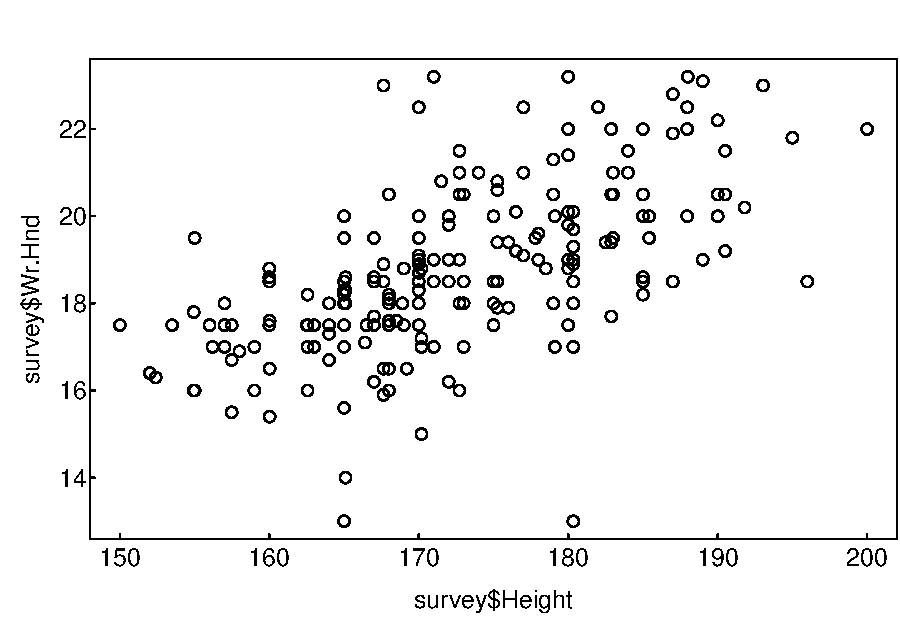
\includegraphics[width=0.6\linewidth]{03_Getting_started_with_a_data_analaysis_files/figure-latex/unnamed-chunk-51-1} \end{center}

There is an equivalent approach for these types of plots which often causes some confusion at first. You can also use the formula notation when using the \texttt{plot()} function. However, in contrast to the previous method the formula method requires you to specify the y axis variable first, then a \texttt{\textasciitilde{}} and then our x axis variable.

\begin{Shaded}
\begin{Highlighting}[]
\FunctionTok{par}\NormalTok{(}\AttributeTok{mar =} \FunctionTok{c}\NormalTok{(}\DecValTok{4}\NormalTok{, }\DecValTok{4}\NormalTok{, }\FloatTok{0.1}\NormalTok{, }\FloatTok{0.1}\NormalTok{))}
\FunctionTok{plot}\NormalTok{(Wr.Hnd}\SpecialCharTok{\textasciitilde{}}\NormalTok{Height, }\AttributeTok{data=}\NormalTok{survey)}
\FunctionTok{plot}\NormalTok{(Wr.Hnd}\SpecialCharTok{\textasciitilde{}}\NormalTok{Height, }\AttributeTok{data=}\NormalTok{survey, }\AttributeTok{col=}\NormalTok{survey}\SpecialCharTok{$}\NormalTok{Sex, }\AttributeTok{pch=}\DecValTok{16}\NormalTok{)}
\end{Highlighting}
\end{Shaded}

\begin{figure}
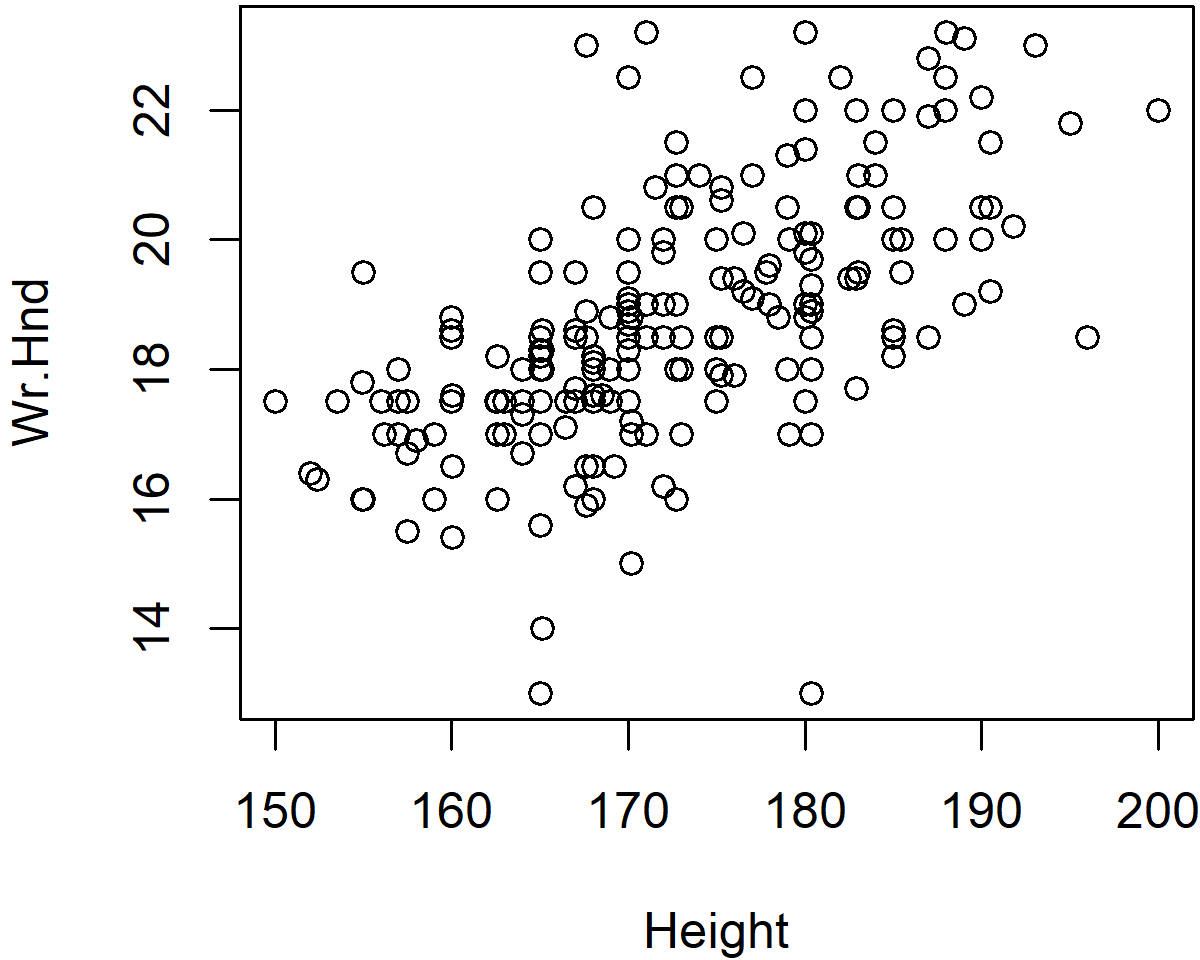
\includegraphics[width=0.5\linewidth]{03_Getting_started_with_a_data_analaysis_files/figure-latex/unnamed-chunk-52-1} 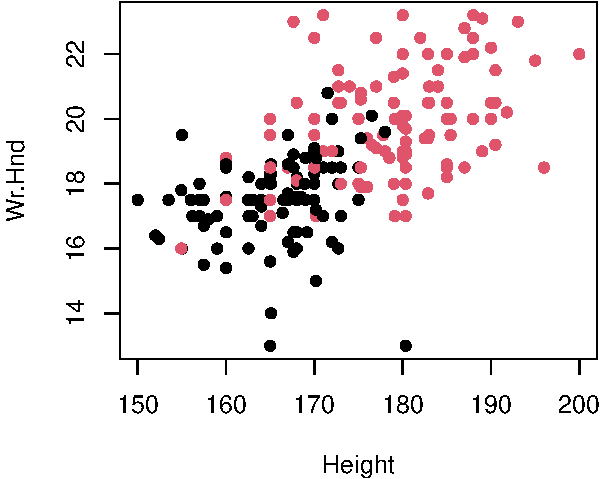
\includegraphics[width=0.5\linewidth]{03_Getting_started_with_a_data_analaysis_files/figure-latex/unnamed-chunk-52-2} \end{figure}

\hypertarget{ggplot2-graphics}{%
\subsection{ggplot2 graphics}\label{ggplot2-graphics}}

ggplot2 graphics is based on \textbf{ggplot2} package. Because \textbf{ggplot2} isn't part of the standard distribution of R, you have to download the package from CRAN and install it. To install the \textbf{ggplot2} package, use:

\begin{Shaded}
\begin{Highlighting}[]
\FunctionTok{install.packages}\NormalTok{(}\StringTok{"ggplot2"}\NormalTok{)}
\end{Highlighting}
\end{Shaded}

And then to load the package, use:

\begin{Shaded}
\begin{Highlighting}[]
\FunctionTok{library}\NormalTok{(}\StringTok{"ggplot2"}\NormalTok{)}
\end{Highlighting}
\end{Shaded}

The basic concept of a ggplot2 graphic is that you combine different plot elements into layers. Each layer of a ggplot2 graphic contains information about the following:

\begin{itemize}
\tightlist
\item
  The data that you want to plot: for \texttt{ggplot()}, this must be a data
  frame.
\item
  A mapping from the data to your plot: this usually is as simple as telling \texttt{ggplot()} what goes on the x‐axis and what goes on the y‐axis.
\item
  A geometric object, or geom in ggplot terminology: the geom defines
  the overall look of the layer (for example, whether the plot is made up of bars, points, or lines).
\end{itemize}

\hypertarget{bar-plot-1}{%
\subsubsection{Bar plot}\label{bar-plot-1}}

Please study carefully the following codes and outputs:

\begin{Shaded}
\begin{Highlighting}[]
\FunctionTok{library}\NormalTok{(ggplot2)}
\FunctionTok{ggplot}\NormalTok{(}\AttributeTok{data =}\NormalTok{ gss}\FloatTok{.2016}\NormalTok{, }\AttributeTok{mapping =} \FunctionTok{aes}\NormalTok{(}\AttributeTok{x=}\NormalTok{age.f)) }\SpecialCharTok{+} \FunctionTok{geom\_bar}\NormalTok{()}
\FunctionTok{ggplot}\NormalTok{(}\AttributeTok{data =}\NormalTok{ gss}\FloatTok{.2016}\NormalTok{, }\AttributeTok{mapping =} \FunctionTok{aes}\NormalTok{(}\AttributeTok{x=}\NormalTok{grass)) }\SpecialCharTok{+} \FunctionTok{geom\_bar}\NormalTok{()}
\end{Highlighting}
\end{Shaded}

\begin{figure}
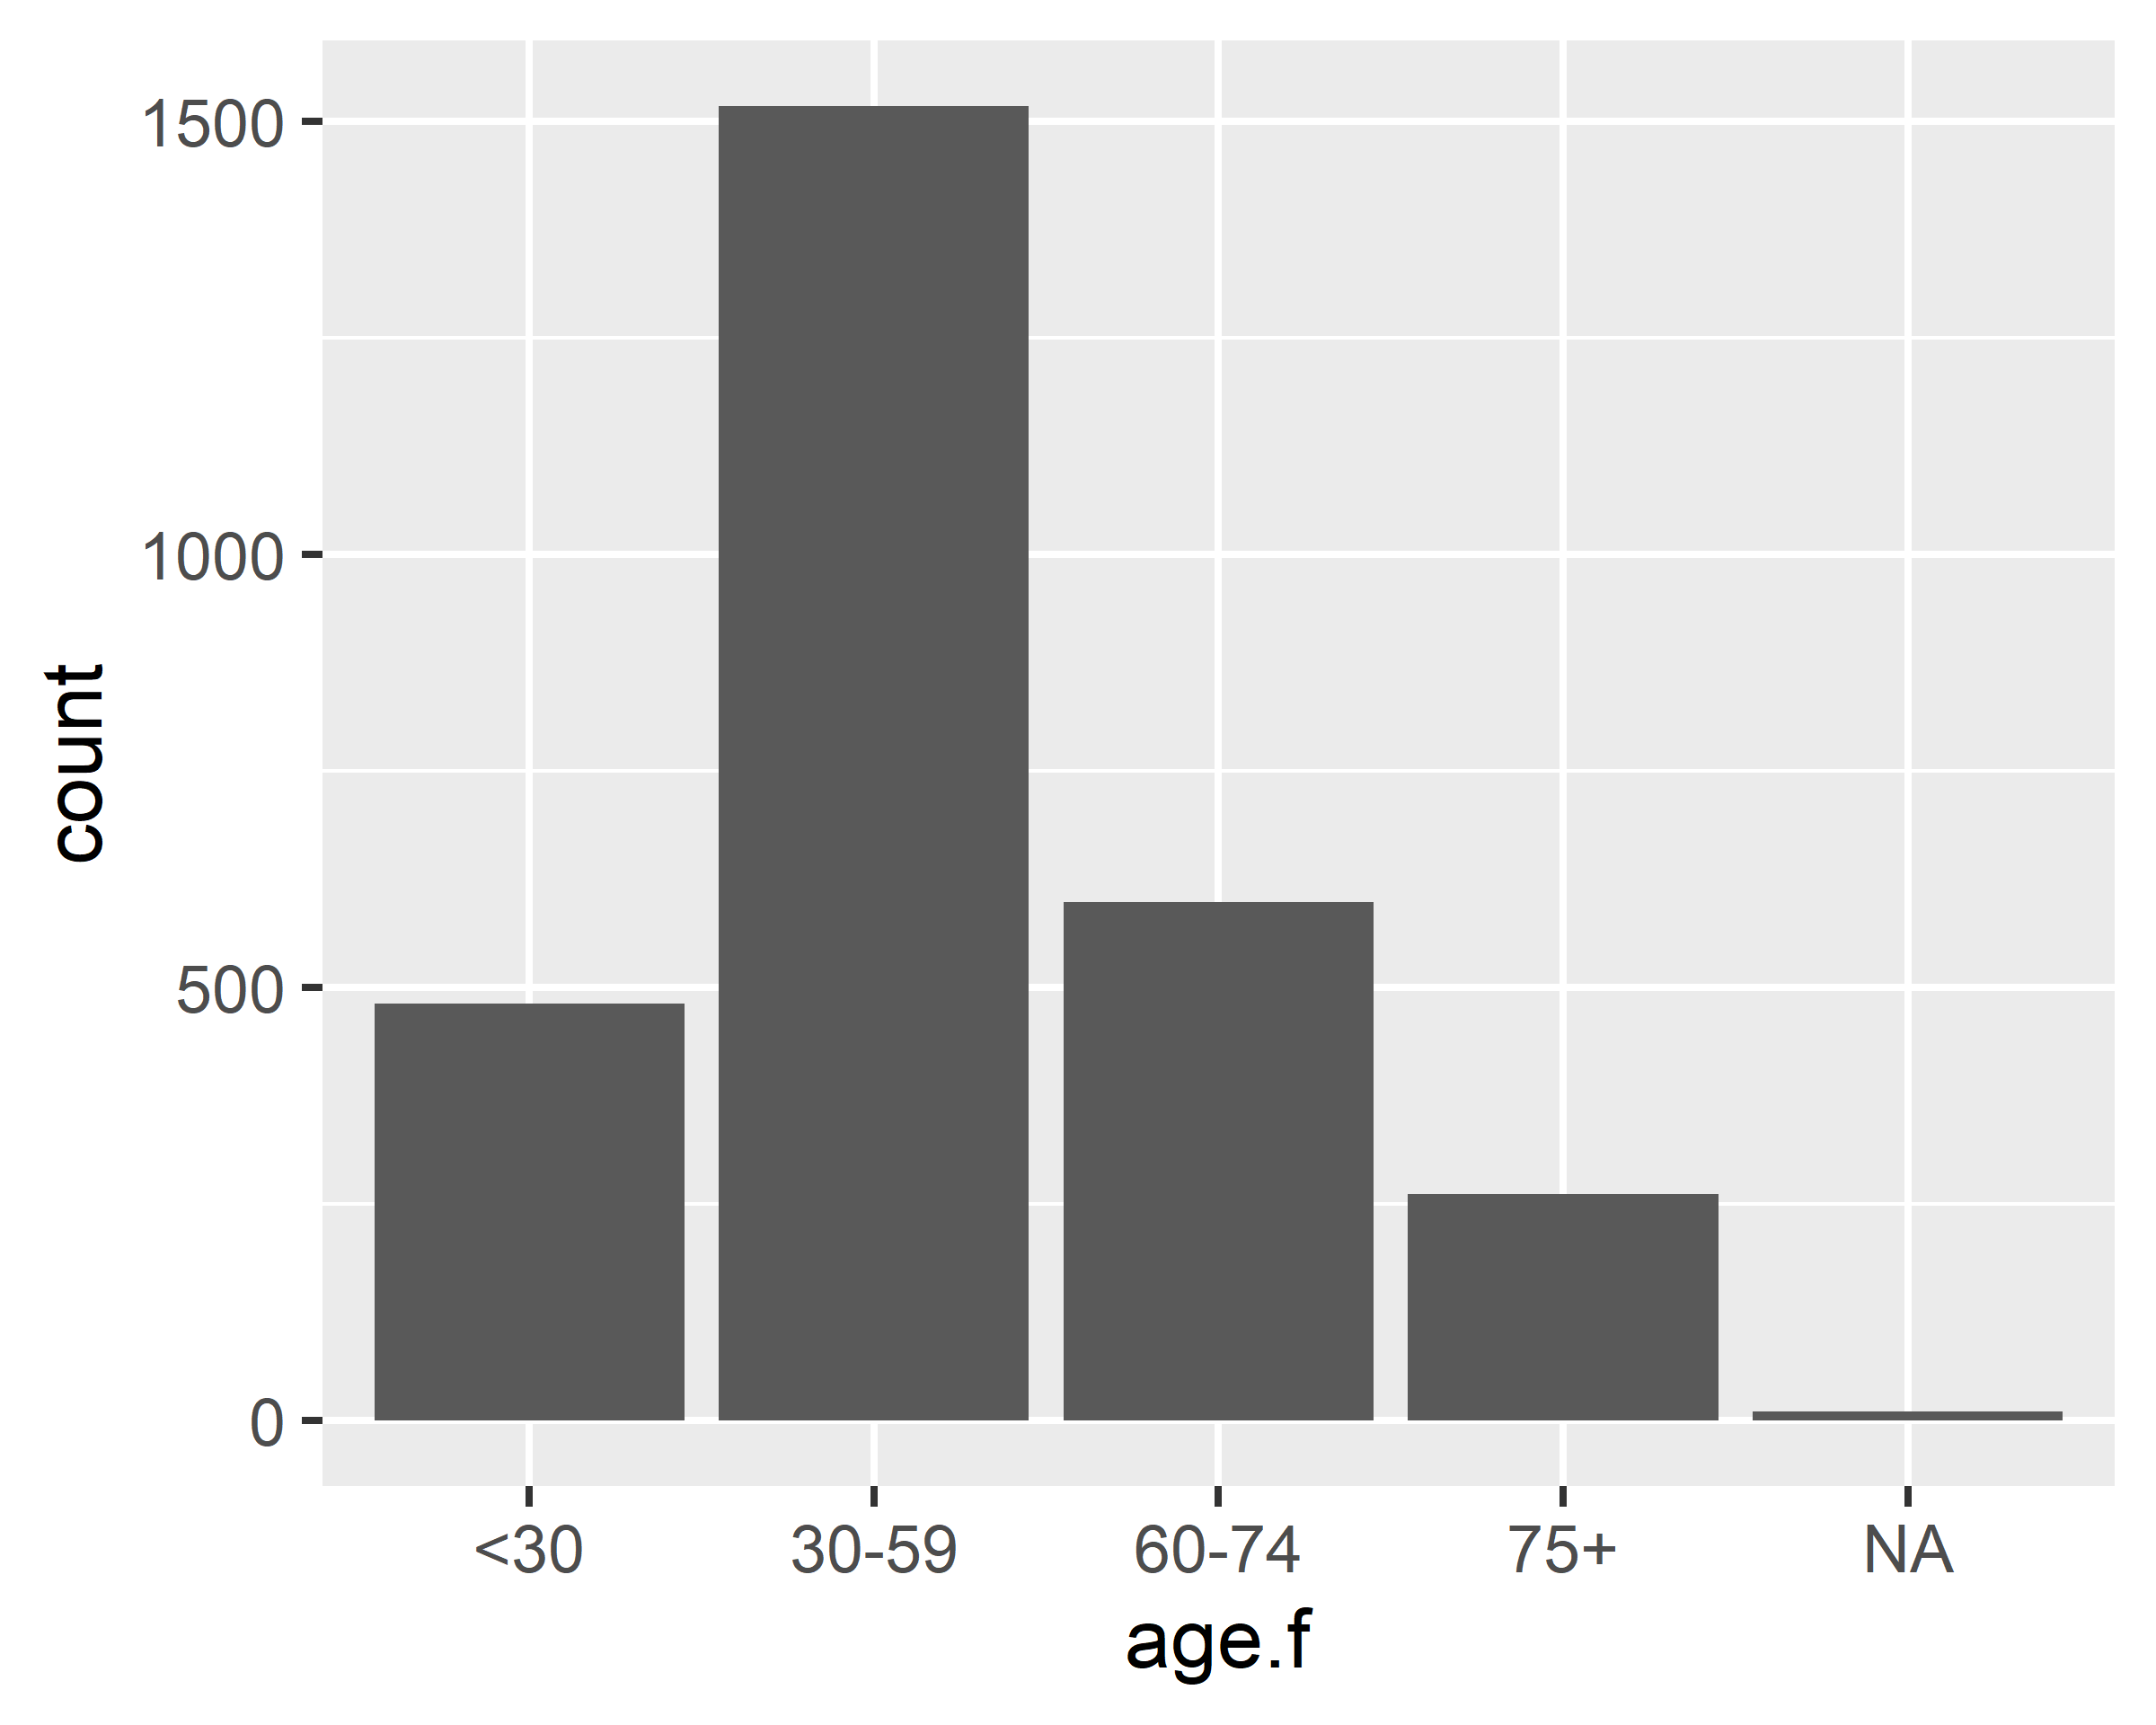
\includegraphics[width=0.5\linewidth]{03_Getting_started_with_a_data_analaysis_files/figure-latex/unnamed-chunk-55-1} 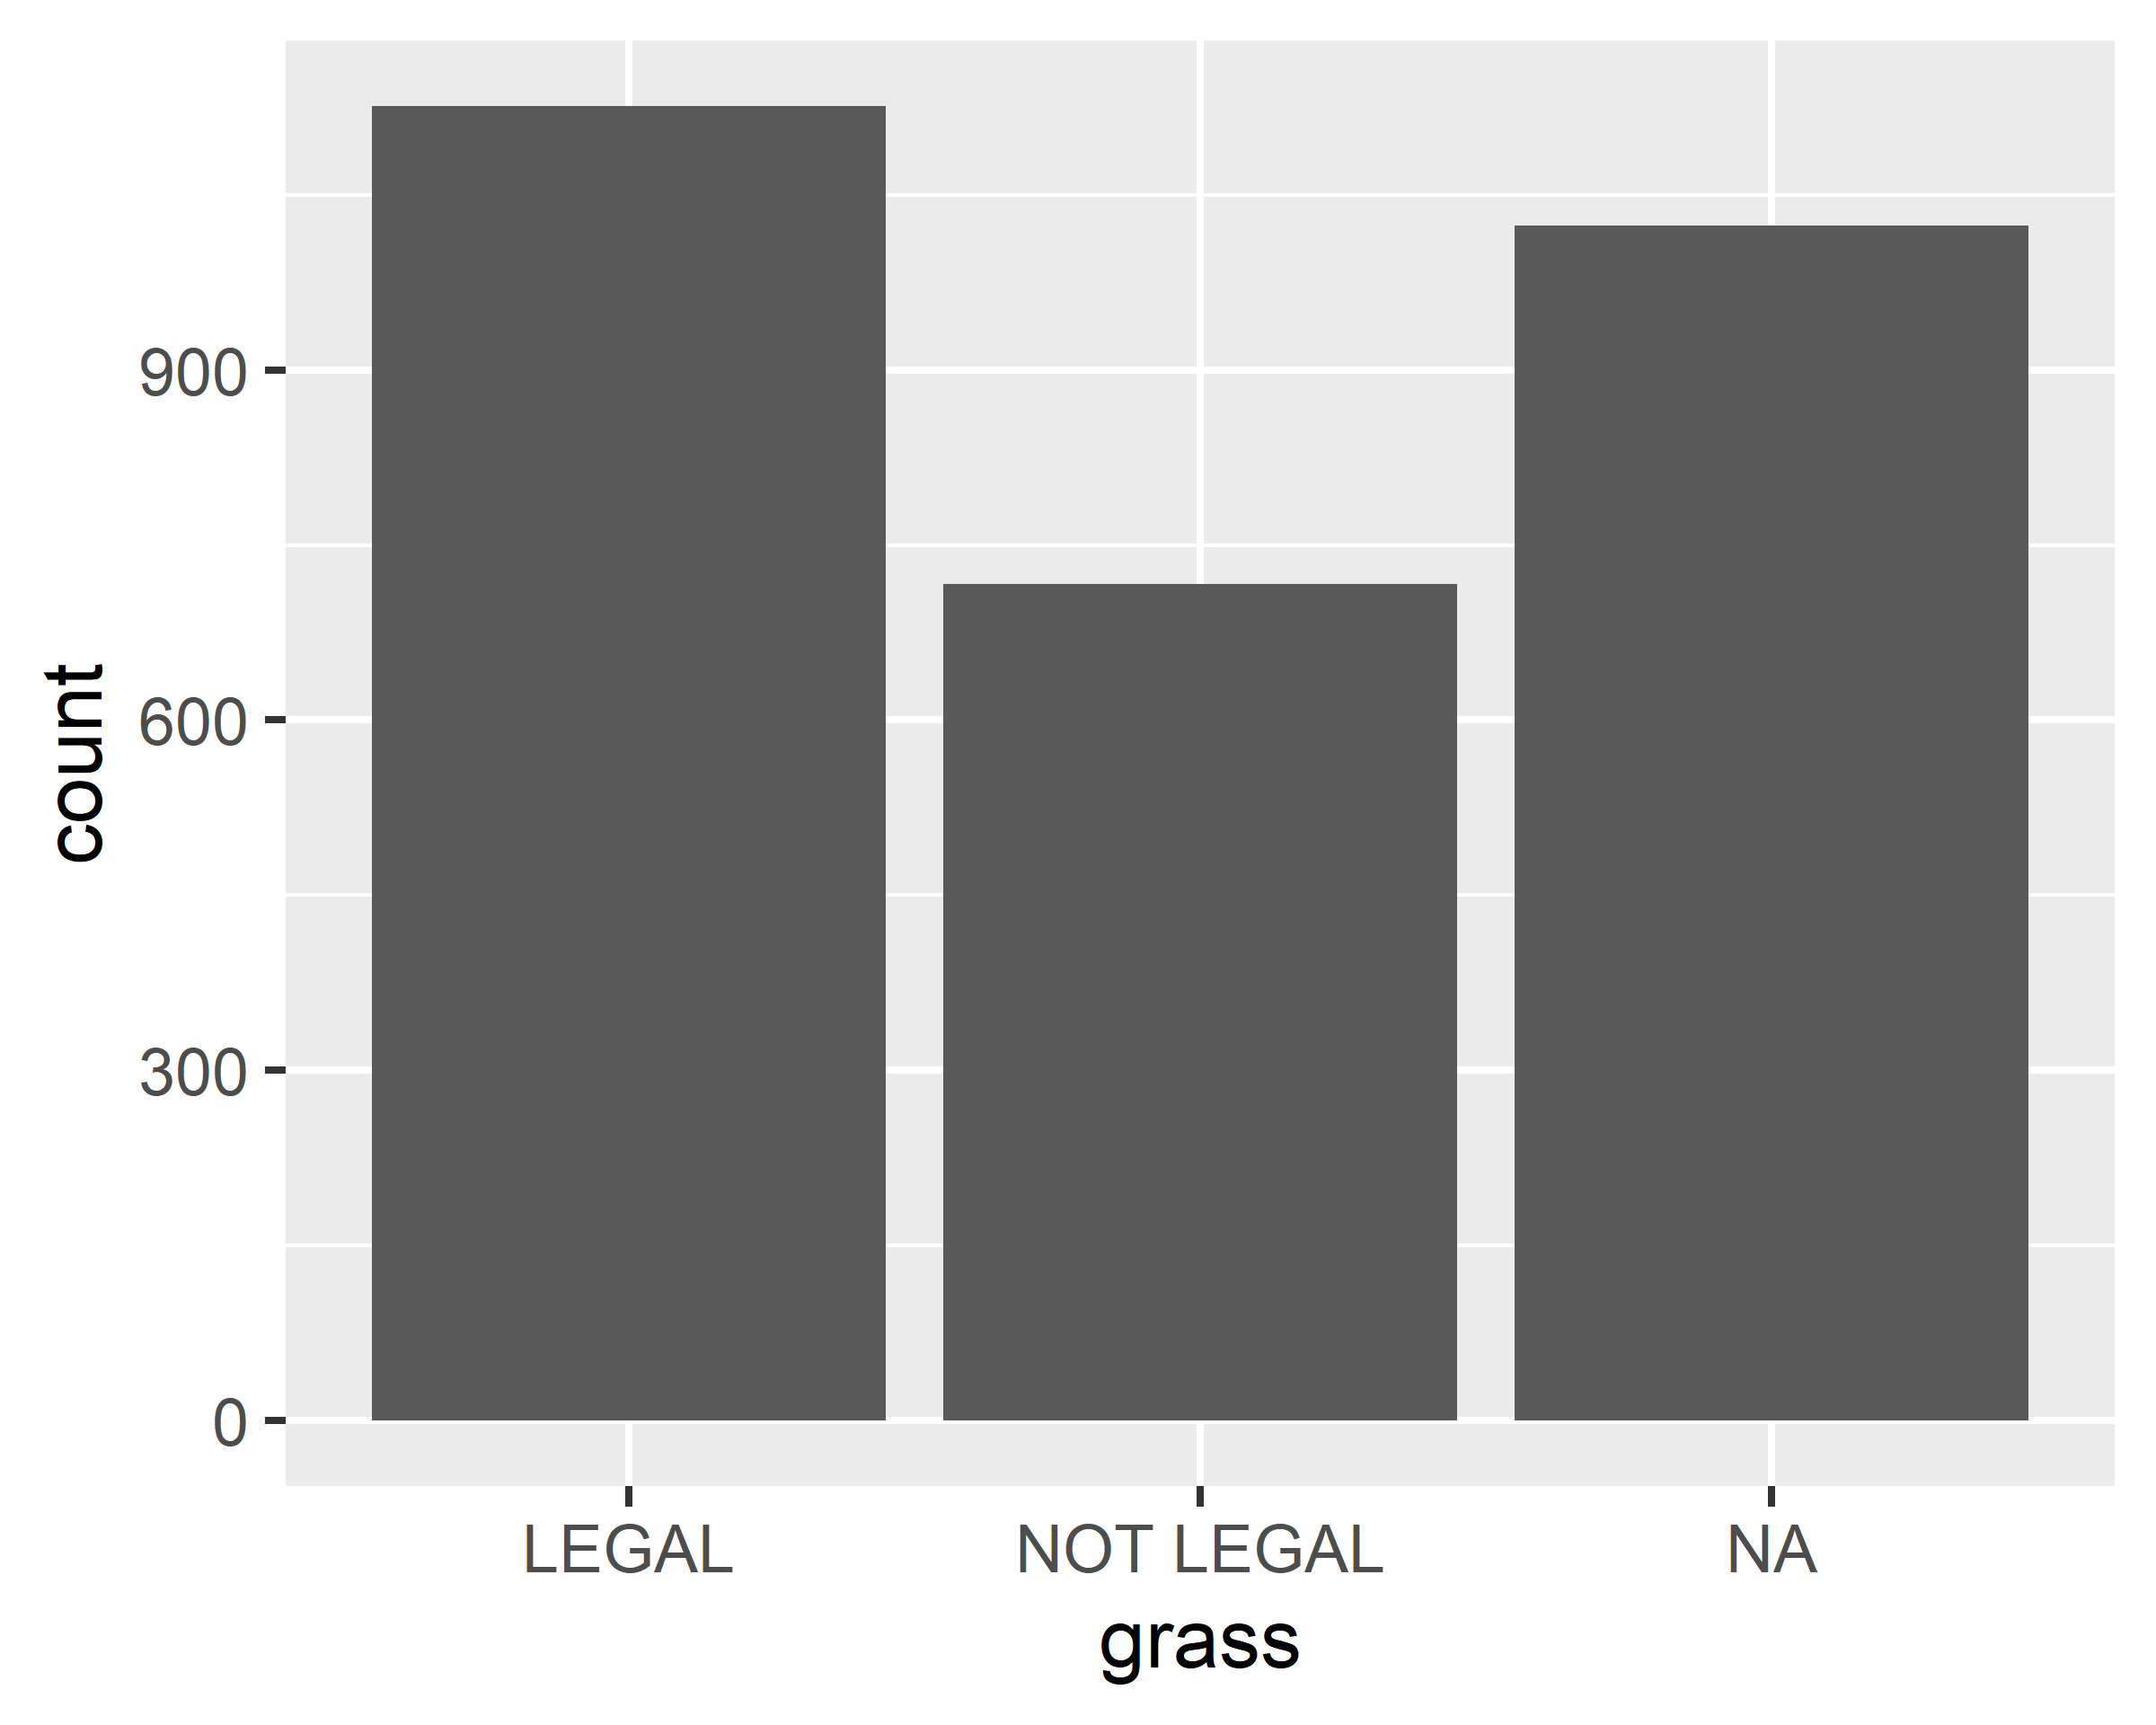
\includegraphics[width=0.5\linewidth]{03_Getting_started_with_a_data_analaysis_files/figure-latex/unnamed-chunk-55-2} \end{figure}

\begin{Shaded}
\begin{Highlighting}[]
\FunctionTok{ggplot}\NormalTok{(}\AttributeTok{data =}\NormalTok{ gss}\FloatTok{.2016}\NormalTok{, }\AttributeTok{mapping =} \FunctionTok{aes}\NormalTok{(}\AttributeTok{x=}\NormalTok{age.f)) }\SpecialCharTok{+} \FunctionTok{geom\_bar}\NormalTok{() }\SpecialCharTok{+} 
  \FunctionTok{scale\_x\_discrete}\NormalTok{(}\AttributeTok{na.translate =}\NormalTok{ F)}
\FunctionTok{ggplot}\NormalTok{(}\AttributeTok{data =}\NormalTok{ gss}\FloatTok{.2016}\NormalTok{, }\AttributeTok{mapping =} \FunctionTok{aes}\NormalTok{(}\AttributeTok{x=}\NormalTok{grass)) }\SpecialCharTok{+} \FunctionTok{geom\_bar}\NormalTok{() }\SpecialCharTok{+} 
  \FunctionTok{scale\_x\_discrete}\NormalTok{(}\AttributeTok{na.translate =}\NormalTok{ F)}
\end{Highlighting}
\end{Shaded}

\begin{figure}
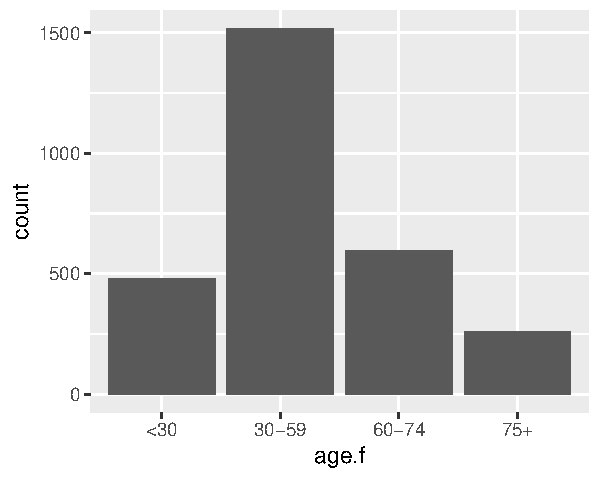
\includegraphics[width=0.5\linewidth]{03_Getting_started_with_a_data_analaysis_files/figure-latex/unnamed-chunk-56-1} 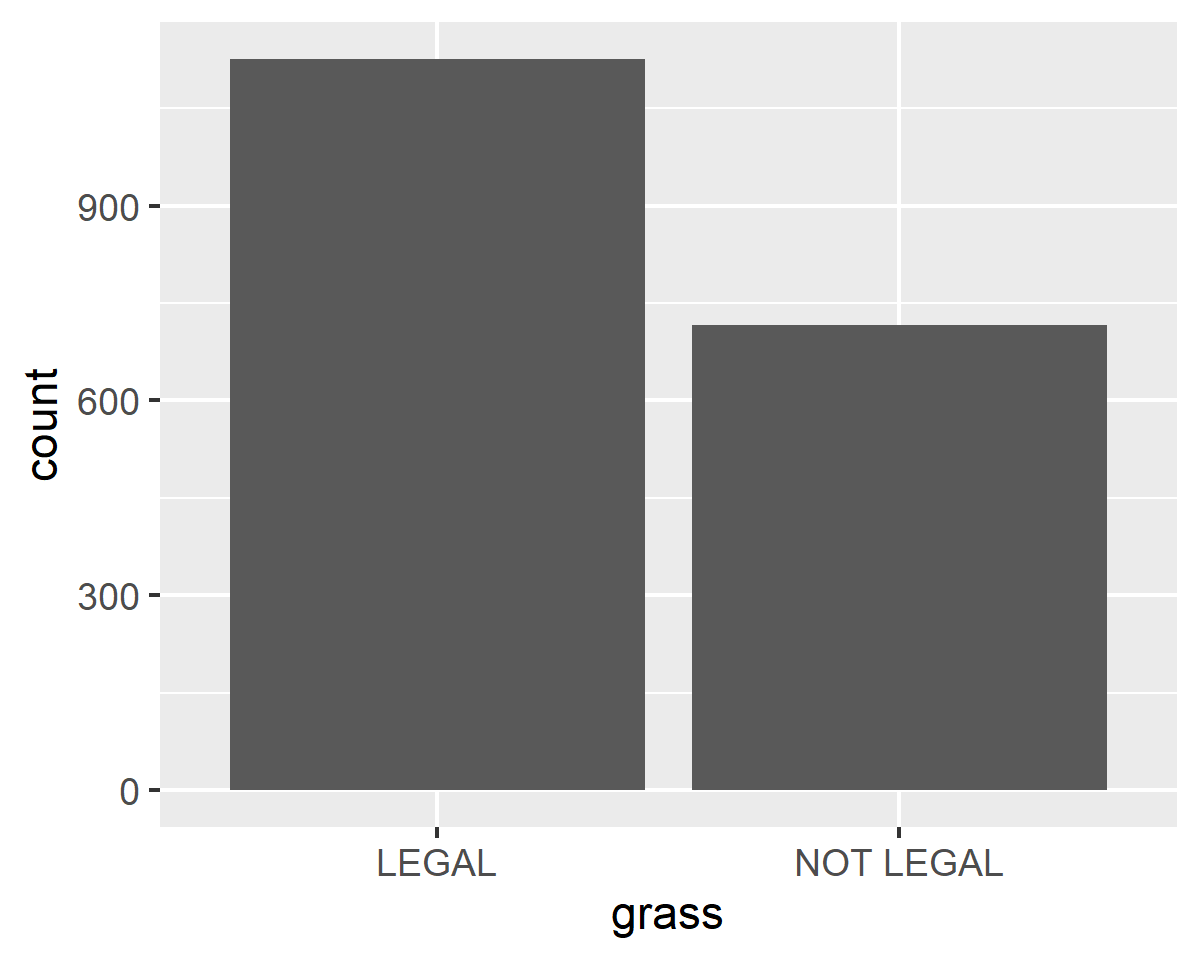
\includegraphics[width=0.5\linewidth]{03_Getting_started_with_a_data_analaysis_files/figure-latex/unnamed-chunk-56-2} \end{figure}

\begin{Shaded}
\begin{Highlighting}[]
\FunctionTok{ggplot}\NormalTok{(}\AttributeTok{data =}\NormalTok{ gss}\FloatTok{.2016}\NormalTok{, }\AttributeTok{mapping =} \FunctionTok{aes}\NormalTok{(}\AttributeTok{x=}\NormalTok{age.f, }\AttributeTok{fill=}\NormalTok{age.f)) }\SpecialCharTok{+} \FunctionTok{geom\_bar}\NormalTok{() }\SpecialCharTok{+} 
  \FunctionTok{scale\_x\_discrete}\NormalTok{(}\AttributeTok{na.translate =}\NormalTok{ F)}
\FunctionTok{ggplot}\NormalTok{(}\AttributeTok{data =}\NormalTok{ gss}\FloatTok{.2016}\NormalTok{, }\AttributeTok{mapping =} \FunctionTok{aes}\NormalTok{(}\AttributeTok{x=}\NormalTok{grass, }\AttributeTok{fill=}\NormalTok{grass)) }\SpecialCharTok{+} \FunctionTok{geom\_bar}\NormalTok{() }\SpecialCharTok{+} 
  \FunctionTok{scale\_x\_discrete}\NormalTok{(}\AttributeTok{na.translate =}\NormalTok{ F)}
\end{Highlighting}
\end{Shaded}

\begin{figure}
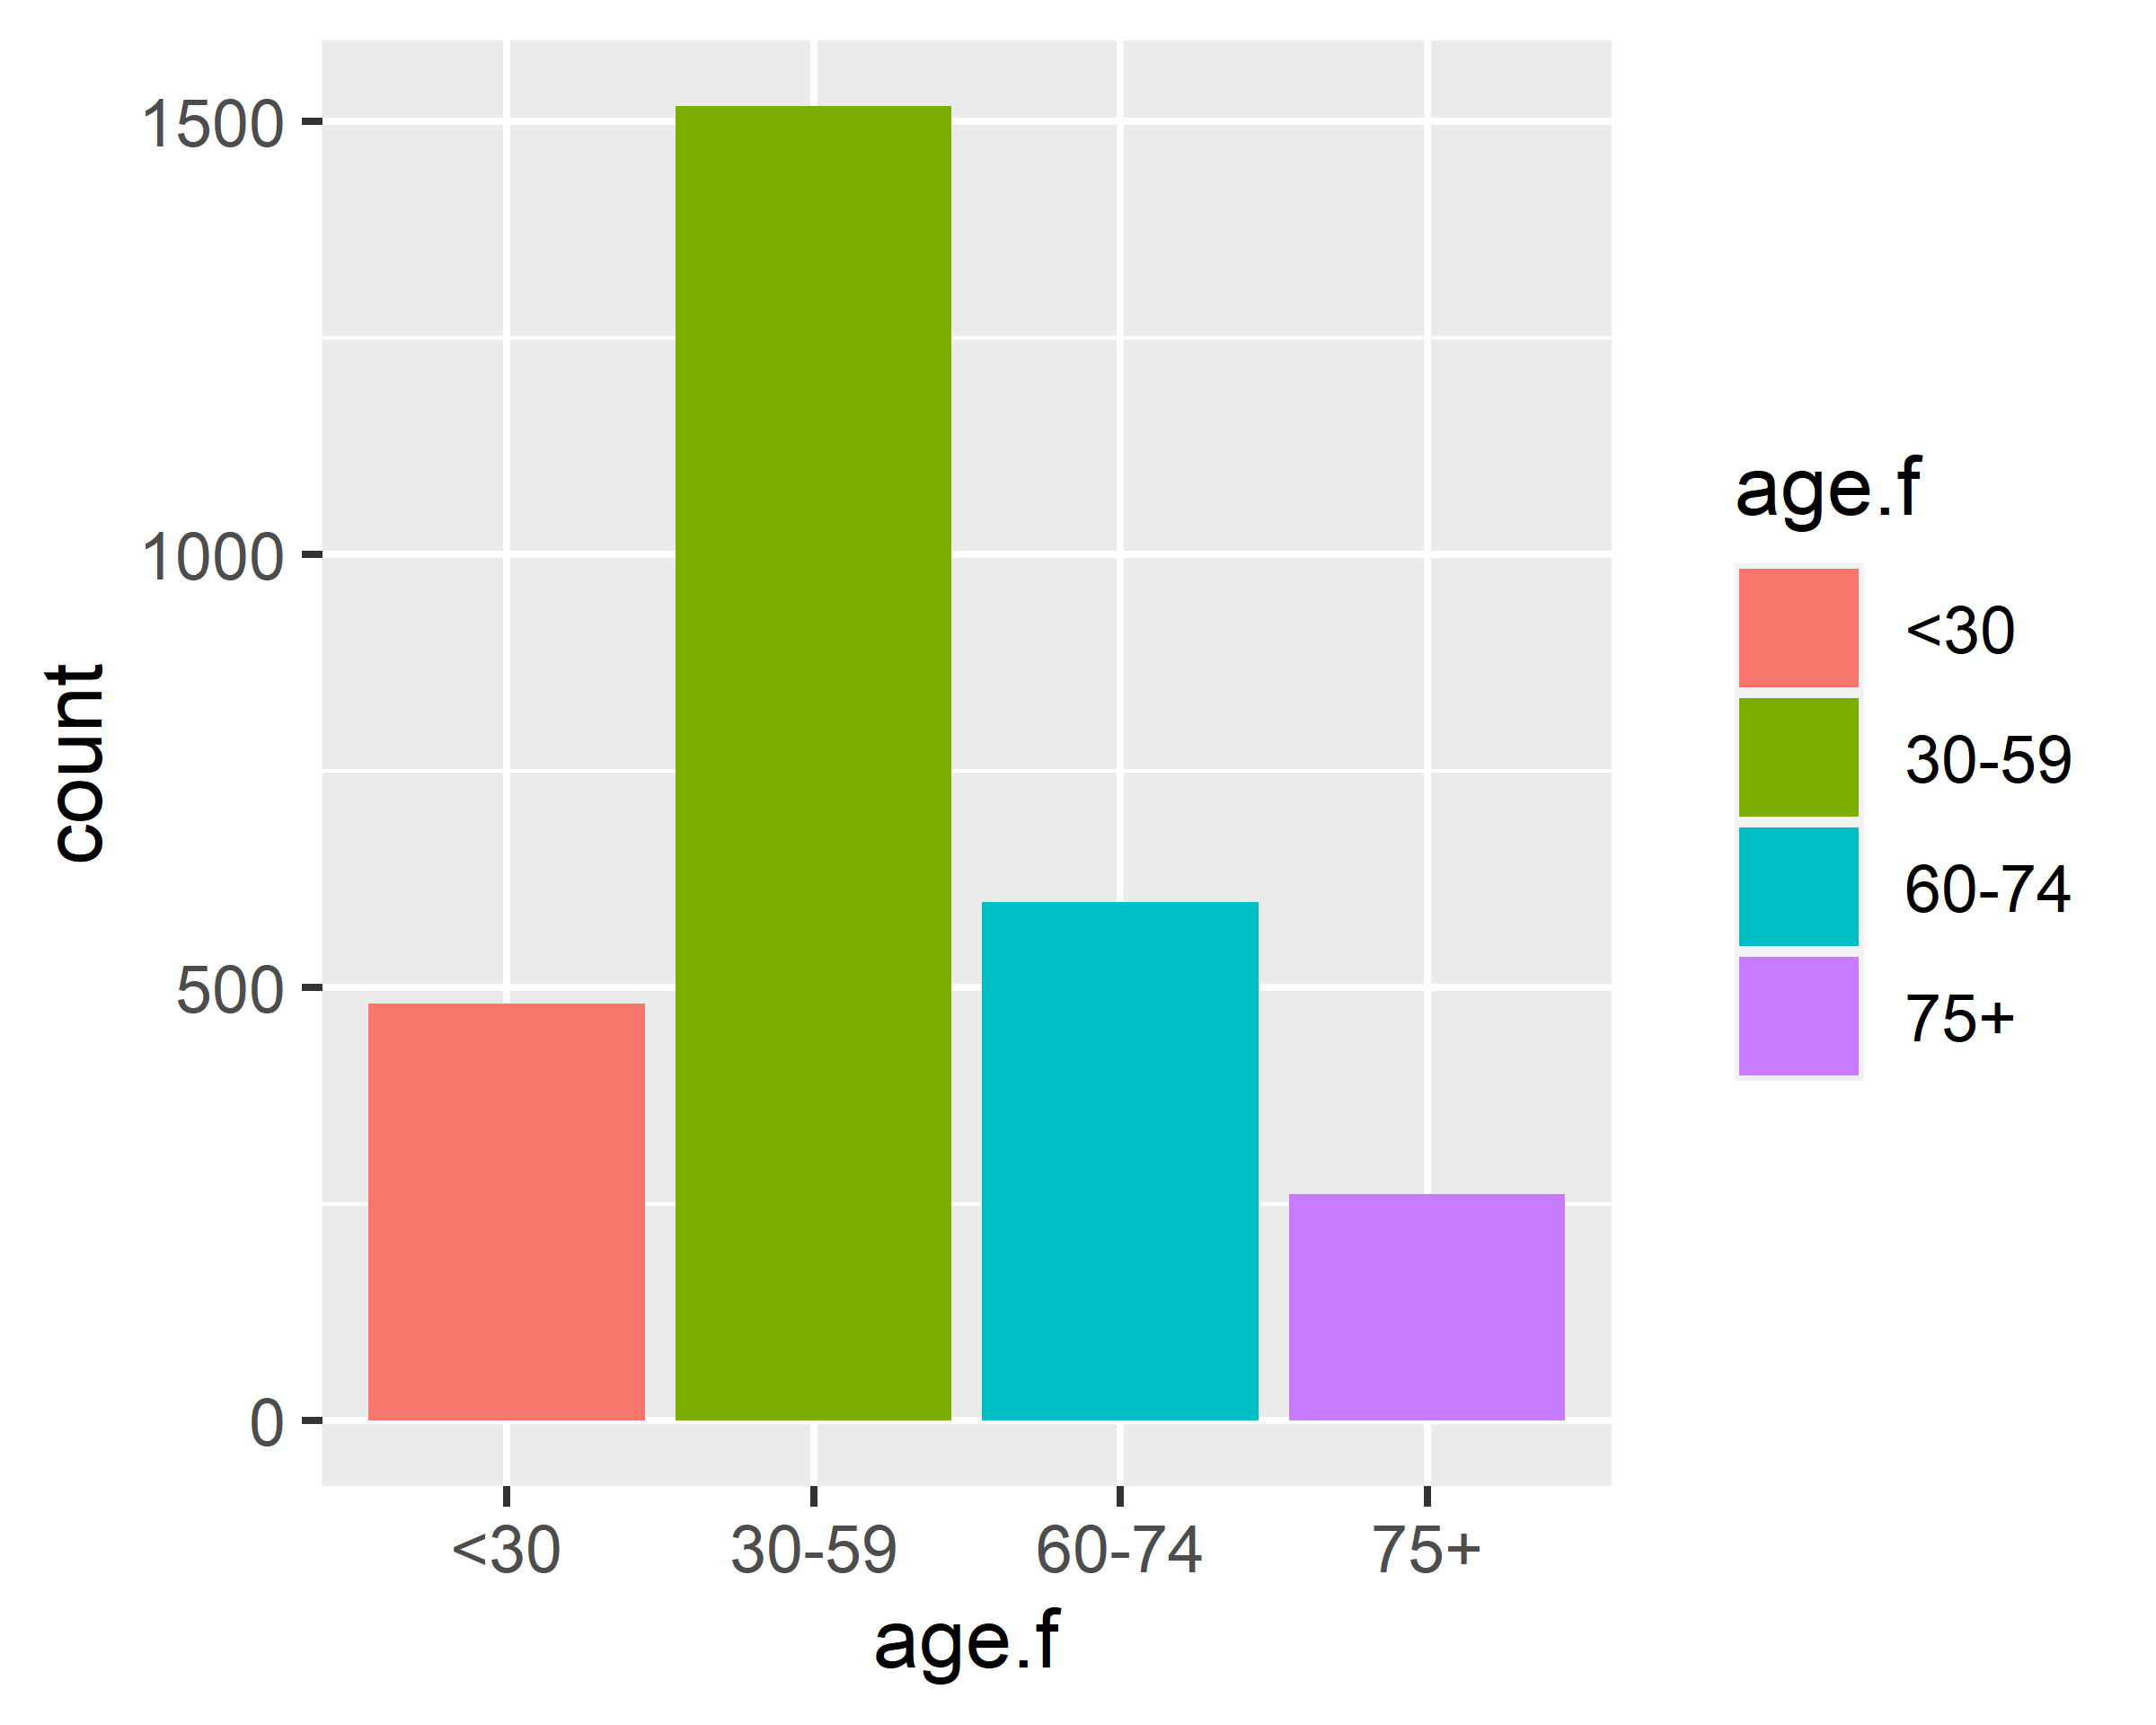
\includegraphics[width=0.5\linewidth]{03_Getting_started_with_a_data_analaysis_files/figure-latex/unnamed-chunk-57-1} 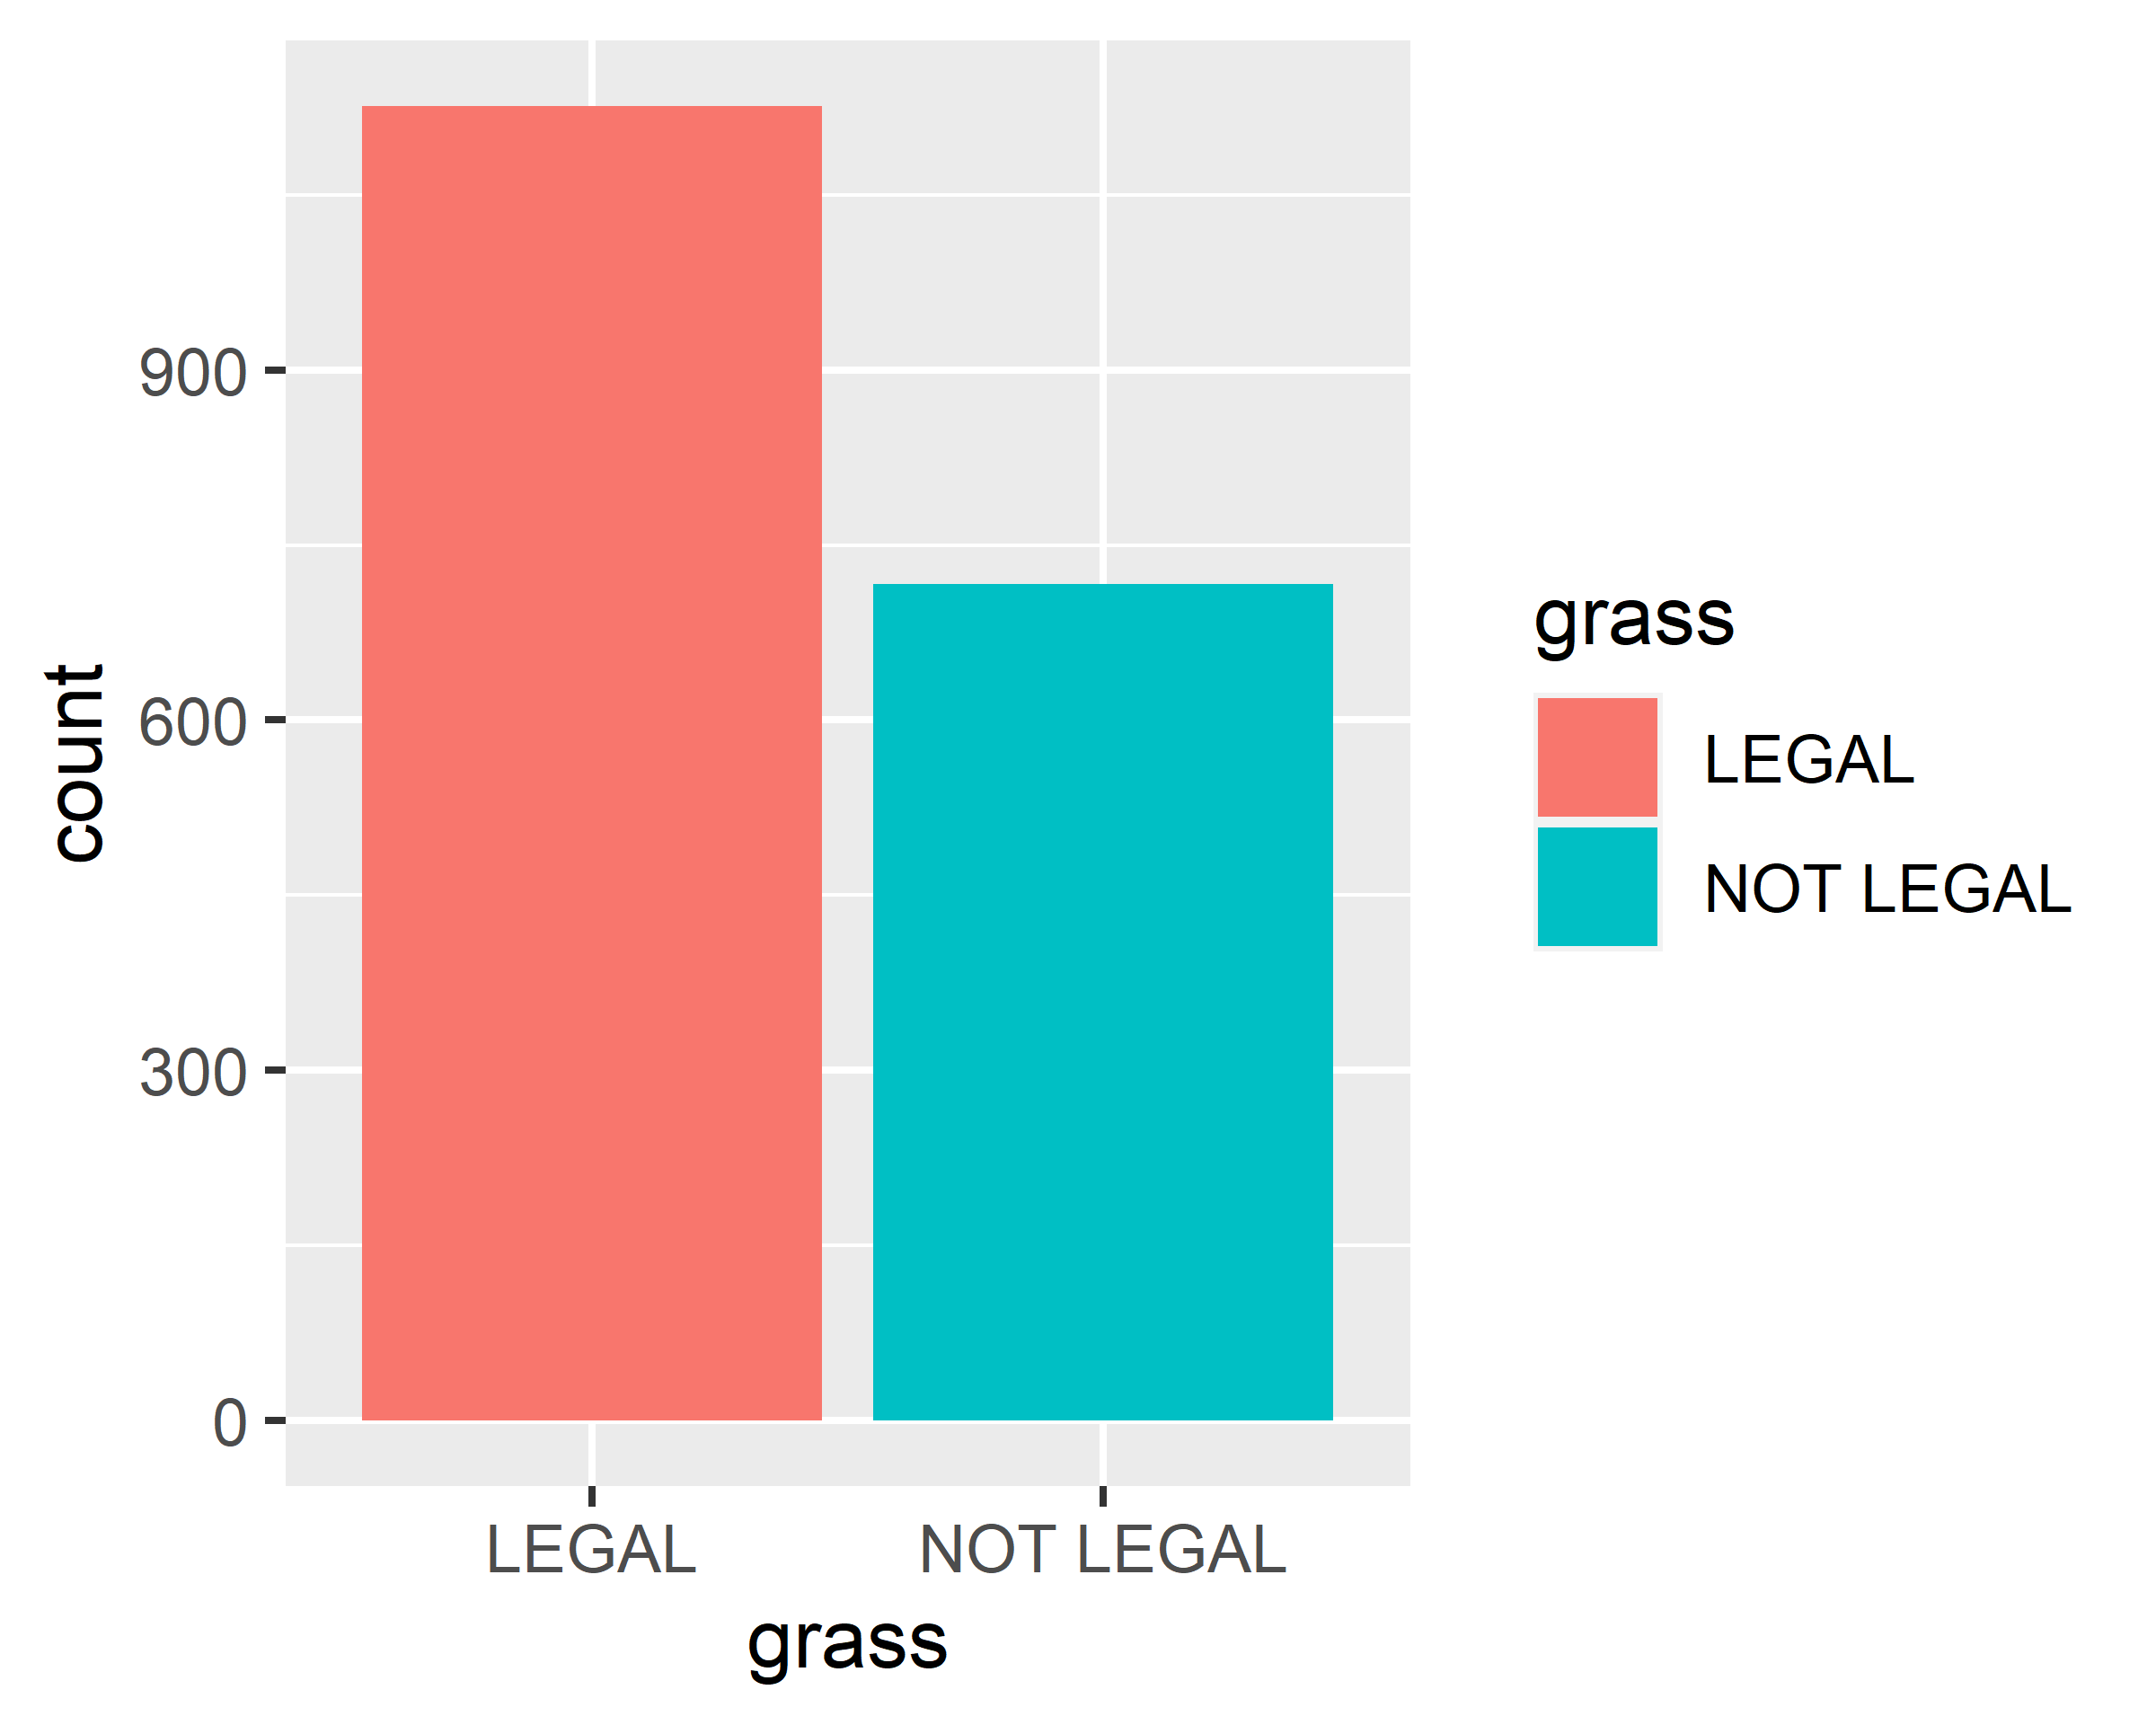
\includegraphics[width=0.5\linewidth]{03_Getting_started_with_a_data_analaysis_files/figure-latex/unnamed-chunk-57-2} \end{figure}

\begin{Shaded}
\begin{Highlighting}[]
\FunctionTok{ggplot}\NormalTok{(}\AttributeTok{data =}\NormalTok{ gss}\FloatTok{.2016}\NormalTok{, }\AttributeTok{mapping =} \FunctionTok{aes}\NormalTok{(}\AttributeTok{x=}\NormalTok{grass, }\AttributeTok{fill=}\NormalTok{grass)) }\SpecialCharTok{+} \FunctionTok{geom\_bar}\NormalTok{() }\SpecialCharTok{+} 
  \FunctionTok{scale\_x\_discrete}\NormalTok{(}\AttributeTok{na.translate =}\NormalTok{ F) }\SpecialCharTok{+} 
  \FunctionTok{scale\_fill\_manual}\NormalTok{(}\AttributeTok{values =} \FunctionTok{c}\NormalTok{(}\StringTok{"\#78A678"}\NormalTok{, }\StringTok{"\#7463AC"}\NormalTok{), }\AttributeTok{guide=}\NormalTok{F)}

\FunctionTok{ggplot}\NormalTok{(}\AttributeTok{data =}\NormalTok{ gss}\FloatTok{.2016}\NormalTok{, }\AttributeTok{mapping =} \FunctionTok{aes}\NormalTok{(}\AttributeTok{x=}\NormalTok{grass, }\AttributeTok{fill=}\NormalTok{grass)) }\SpecialCharTok{+} \FunctionTok{geom\_bar}\NormalTok{() }\SpecialCharTok{+} 
  \FunctionTok{scale\_x\_discrete}\NormalTok{(}\AttributeTok{na.translate =}\NormalTok{ F) }\SpecialCharTok{+} 
  \FunctionTok{scale\_fill\_manual}\NormalTok{(}\AttributeTok{values =} \FunctionTok{c}\NormalTok{(}\StringTok{"\#78A678"}\NormalTok{, }\StringTok{"\#7463AC"}\NormalTok{), }\AttributeTok{guide=}\NormalTok{F) }\SpecialCharTok{+} 
  \FunctionTok{theme\_minimal}\NormalTok{() }\SpecialCharTok{+} 
  \FunctionTok{labs}\NormalTok{(}\AttributeTok{x=}\StringTok{"Should marijuana be legal?"}\NormalTok{, }\AttributeTok{y=}\StringTok{"Number of responses"}\NormalTok{)}
\end{Highlighting}
\end{Shaded}

\begin{figure}
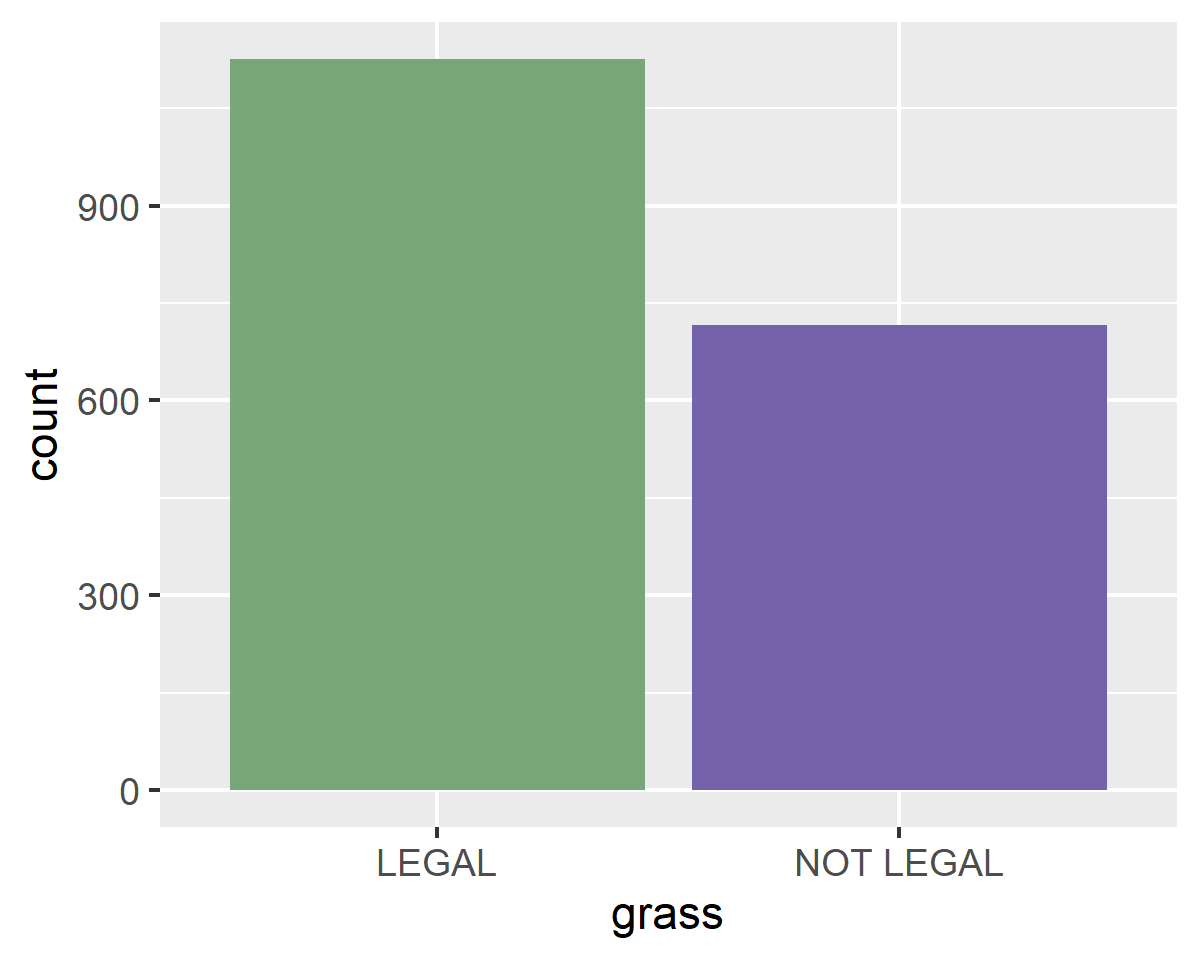
\includegraphics[width=0.5\linewidth]{03_Getting_started_with_a_data_analaysis_files/figure-latex/unnamed-chunk-58-1} 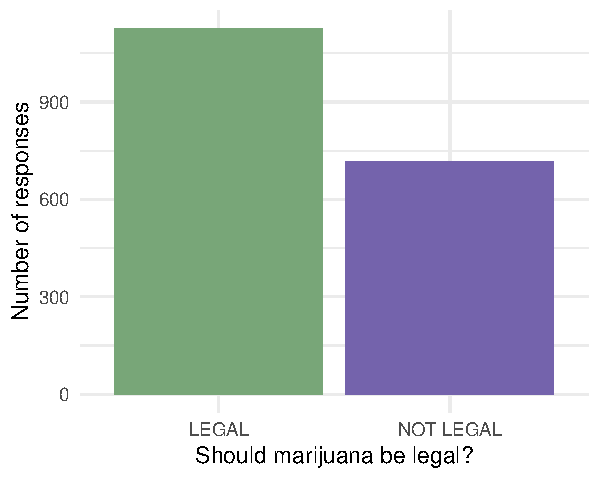
\includegraphics[width=0.5\linewidth]{03_Getting_started_with_a_data_analaysis_files/figure-latex/unnamed-chunk-58-2} \end{figure}

\begin{Shaded}
\begin{Highlighting}[]
\FunctionTok{ggplot}\NormalTok{(}\AttributeTok{data =}\NormalTok{ gss}\FloatTok{.2016}\NormalTok{[}\SpecialCharTok{!}\FunctionTok{is.na}\NormalTok{(gss}\FloatTok{.2016}\SpecialCharTok{$}\NormalTok{grass),], }
       \AttributeTok{mapping =} \FunctionTok{aes}\NormalTok{(}\AttributeTok{x=}\NormalTok{age.f, }\AttributeTok{fill=}\NormalTok{grass)) }\SpecialCharTok{+} \FunctionTok{geom\_bar}\NormalTok{() }\SpecialCharTok{+} 
  \FunctionTok{scale\_x\_discrete}\NormalTok{(}\AttributeTok{na.translate =}\NormalTok{ F)}

\FunctionTok{ggplot}\NormalTok{(}\AttributeTok{data =}\NormalTok{ gss}\FloatTok{.2016}\NormalTok{[}\SpecialCharTok{!}\FunctionTok{is.na}\NormalTok{(gss}\FloatTok{.2016}\SpecialCharTok{$}\NormalTok{grass),], }
       \AttributeTok{mapping =} \FunctionTok{aes}\NormalTok{(}\AttributeTok{x=}\NormalTok{age.f, }\AttributeTok{fill=}\NormalTok{grass)) }\SpecialCharTok{+} \FunctionTok{geom\_bar}\NormalTok{(}\AttributeTok{position =} \StringTok{"fill"}\NormalTok{) }\SpecialCharTok{+} 
  \FunctionTok{scale\_x\_discrete}\NormalTok{(}\AttributeTok{na.translate =}\NormalTok{ F)}
\end{Highlighting}
\end{Shaded}

\begin{figure}
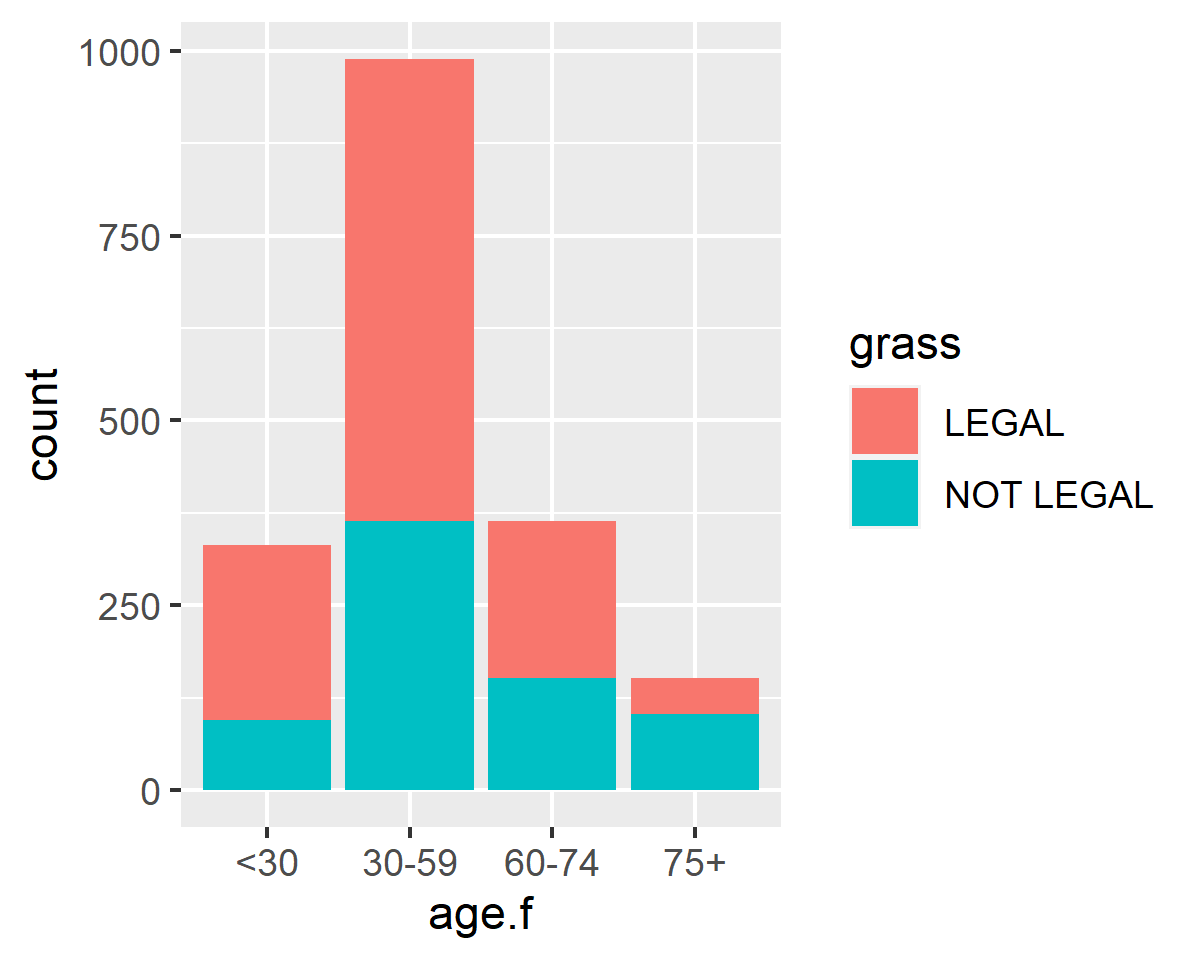
\includegraphics[width=0.5\linewidth]{03_Getting_started_with_a_data_analaysis_files/figure-latex/unnamed-chunk-59-1} 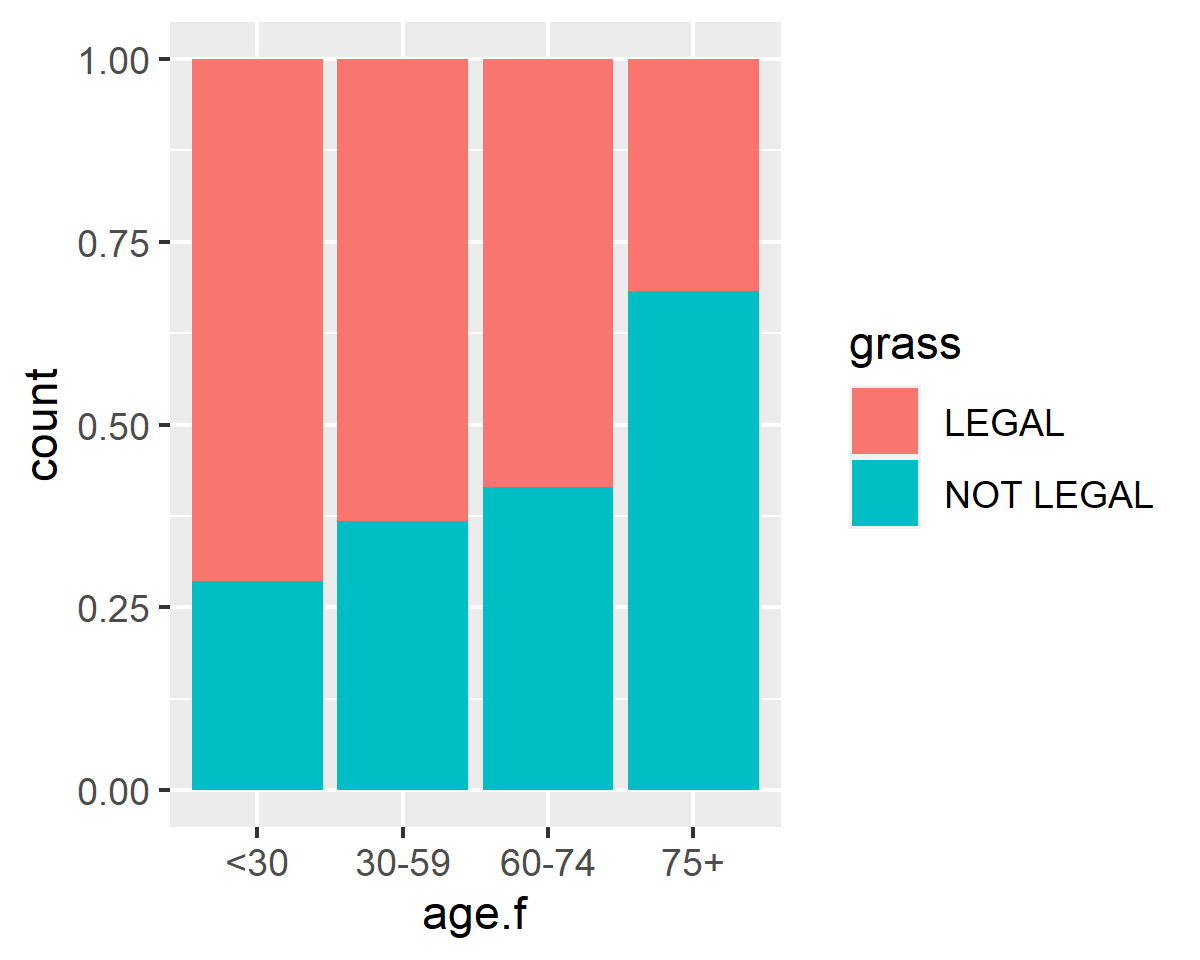
\includegraphics[width=0.5\linewidth]{03_Getting_started_with_a_data_analaysis_files/figure-latex/unnamed-chunk-59-2} \end{figure}

\begin{Shaded}
\begin{Highlighting}[]
\FunctionTok{ggplot}\NormalTok{(}\AttributeTok{data =}\NormalTok{ gss}\FloatTok{.2016}\NormalTok{[}\SpecialCharTok{!}\FunctionTok{is.na}\NormalTok{(gss}\FloatTok{.2016}\SpecialCharTok{$}\NormalTok{grass),], }
       \AttributeTok{mapping =} \FunctionTok{aes}\NormalTok{(}\AttributeTok{x=}\NormalTok{age.f, }\AttributeTok{fill=}\NormalTok{grass)) }\SpecialCharTok{+} \FunctionTok{geom\_bar}\NormalTok{(}\AttributeTok{position =} \StringTok{"dodge"}\NormalTok{) }\SpecialCharTok{+} 
  \FunctionTok{scale\_x\_discrete}\NormalTok{(}\AttributeTok{na.translate =}\NormalTok{ F) }\SpecialCharTok{+} 
    \FunctionTok{labs}\NormalTok{(}\AttributeTok{x=}\StringTok{"Should marijuana be legal?"}\NormalTok{, }\AttributeTok{y=}\StringTok{"Number of responses"}\NormalTok{, }\AttributeTok{fill=}\StringTok{"Legal"}\NormalTok{)}
\FunctionTok{ggplot}\NormalTok{(}\AttributeTok{data =}\NormalTok{ gss}\FloatTok{.2016}\NormalTok{[}\SpecialCharTok{!}\FunctionTok{is.na}\NormalTok{(gss}\FloatTok{.2016}\SpecialCharTok{$}\NormalTok{age.f),], }
       \AttributeTok{mapping =} \FunctionTok{aes}\NormalTok{(}\AttributeTok{x=}\NormalTok{grass, }\AttributeTok{fill=}\NormalTok{age.f)) }\SpecialCharTok{+} \FunctionTok{geom\_bar}\NormalTok{(}\AttributeTok{position =} \StringTok{"dodge"}\NormalTok{) }\SpecialCharTok{+} 
  \FunctionTok{scale\_x\_discrete}\NormalTok{(}\AttributeTok{na.translate =}\NormalTok{ F) }\SpecialCharTok{+} 
    \FunctionTok{labs}\NormalTok{(}\AttributeTok{x=}\StringTok{"Should marijuana be legal?"}\NormalTok{, }\AttributeTok{y=}\StringTok{"Number of responses"}\NormalTok{, }\AttributeTok{fill=}\StringTok{"Age"}\NormalTok{)}
\end{Highlighting}
\end{Shaded}

\begin{figure}
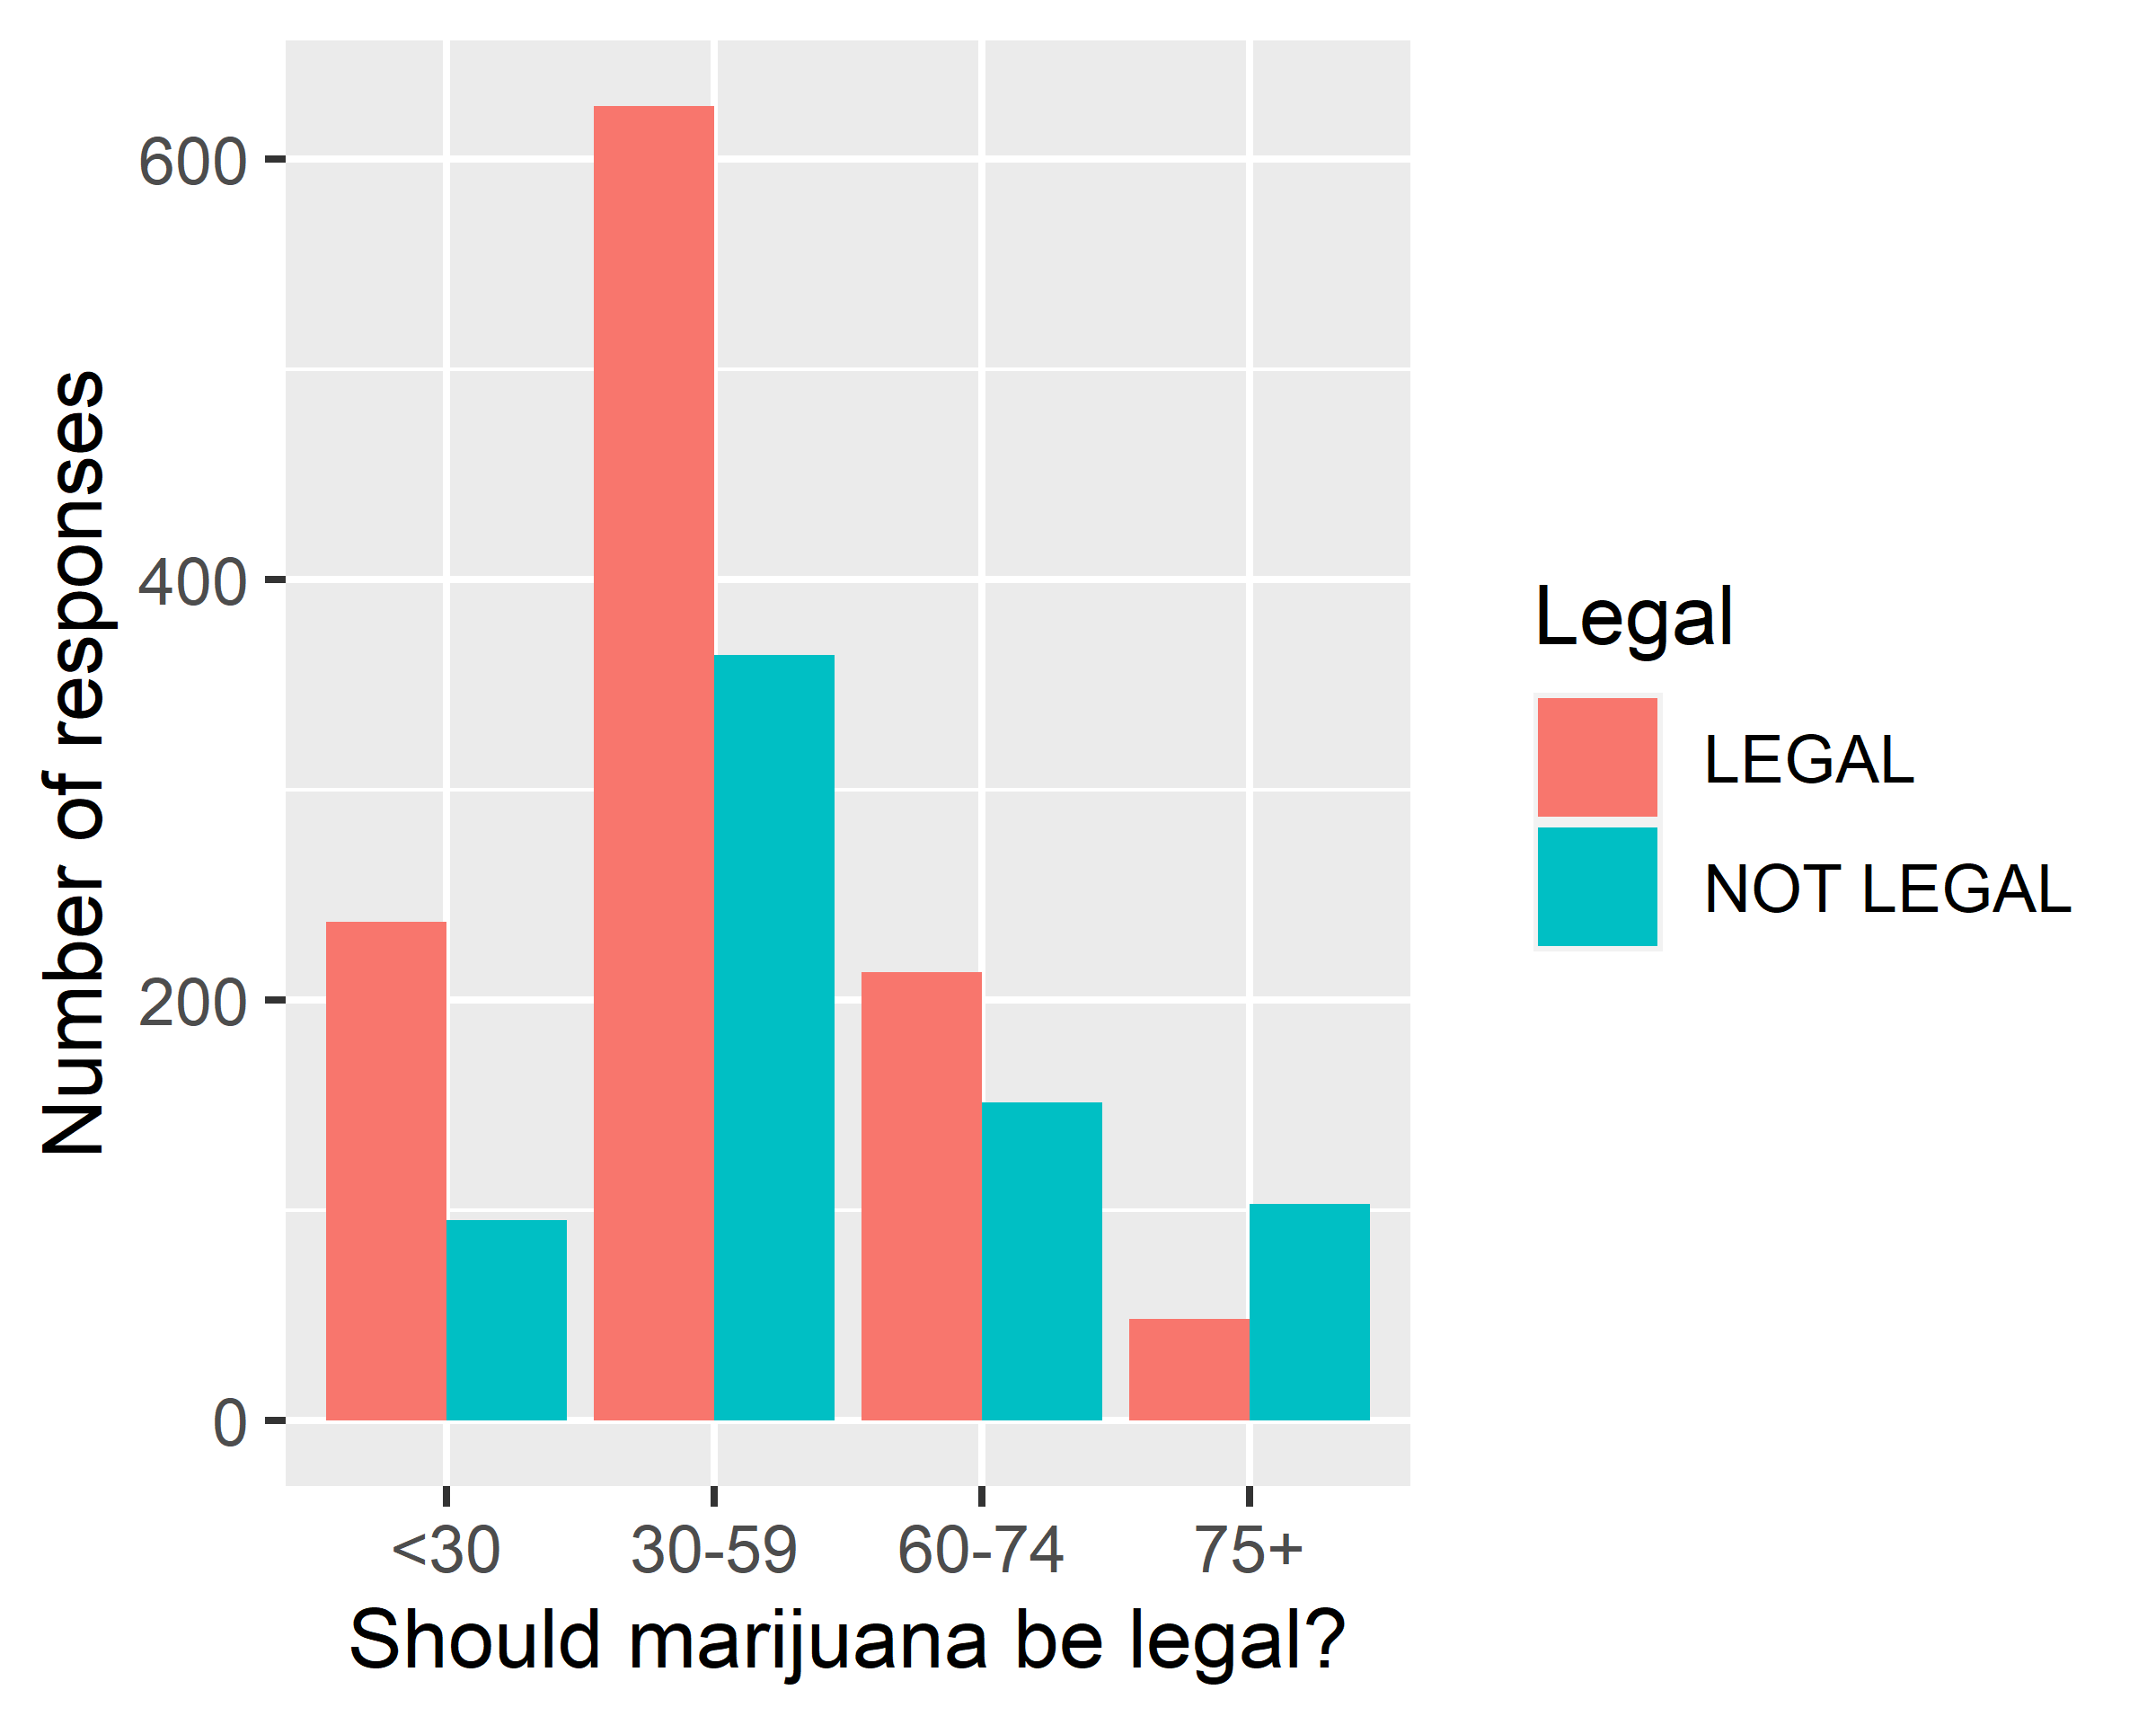
\includegraphics[width=0.5\linewidth]{03_Getting_started_with_a_data_analaysis_files/figure-latex/unnamed-chunk-60-1} 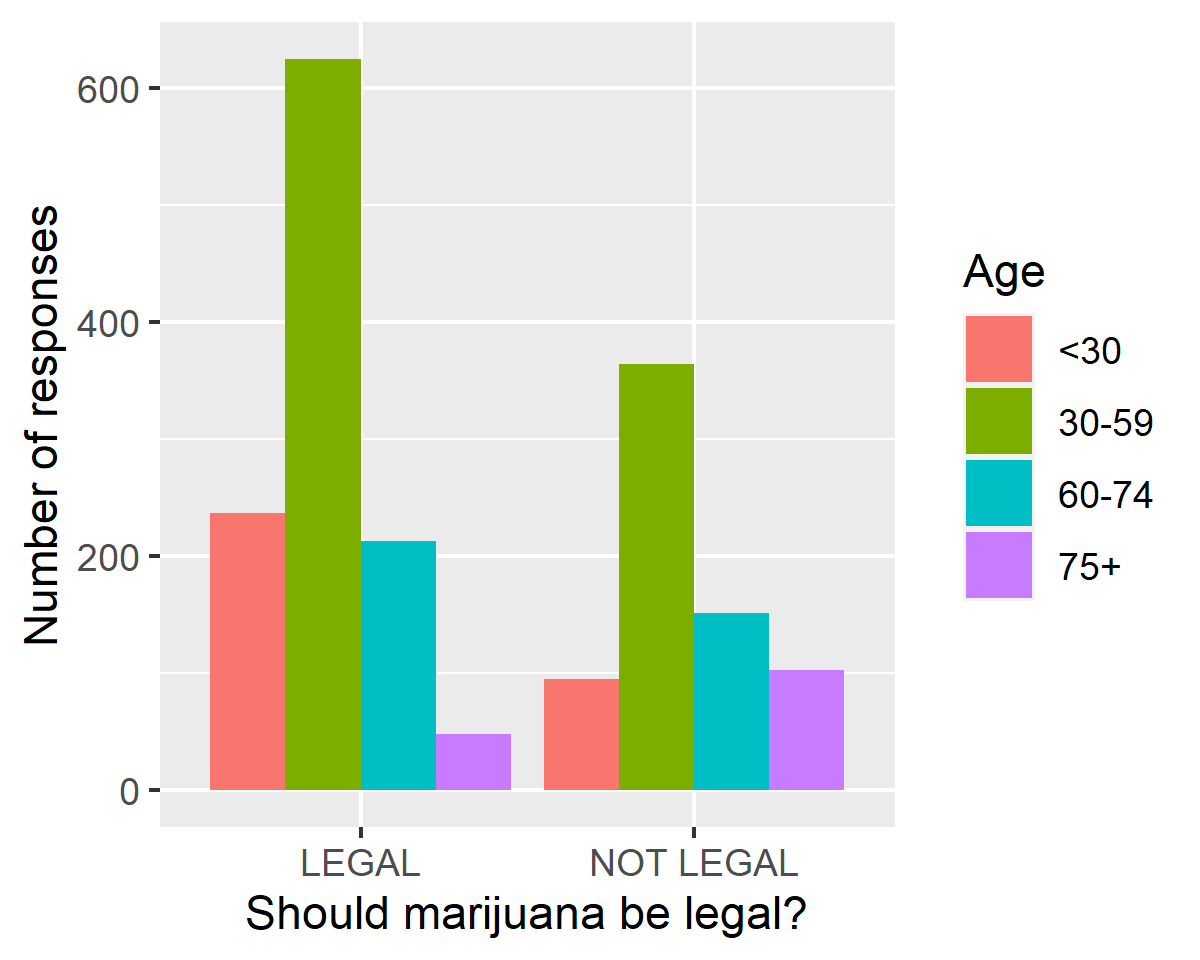
\includegraphics[width=0.5\linewidth]{03_Getting_started_with_a_data_analaysis_files/figure-latex/unnamed-chunk-60-2} \end{figure}

\hypertarget{histogram-1}{%
\subsubsection{Histogram}\label{histogram-1}}

Please study carefully the following codes and outputs:

\begin{Shaded}
\begin{Highlighting}[]
\FunctionTok{ggplot}\NormalTok{(}\AttributeTok{data =}\NormalTok{ survey, }\AttributeTok{mapping =} \FunctionTok{aes}\NormalTok{(}\AttributeTok{x=}\NormalTok{Wr.Hnd)) }\SpecialCharTok{+} \FunctionTok{geom\_histogram}\NormalTok{()}
\FunctionTok{ggplot}\NormalTok{(}\AttributeTok{data =}\NormalTok{ survey, }\AttributeTok{mapping =} \FunctionTok{aes}\NormalTok{(}\AttributeTok{x=}\NormalTok{Wr.Hnd)) }\SpecialCharTok{+} \FunctionTok{geom\_histogram}\NormalTok{(}\AttributeTok{bins =} \DecValTok{10}\NormalTok{)}
\end{Highlighting}
\end{Shaded}

\begin{figure}
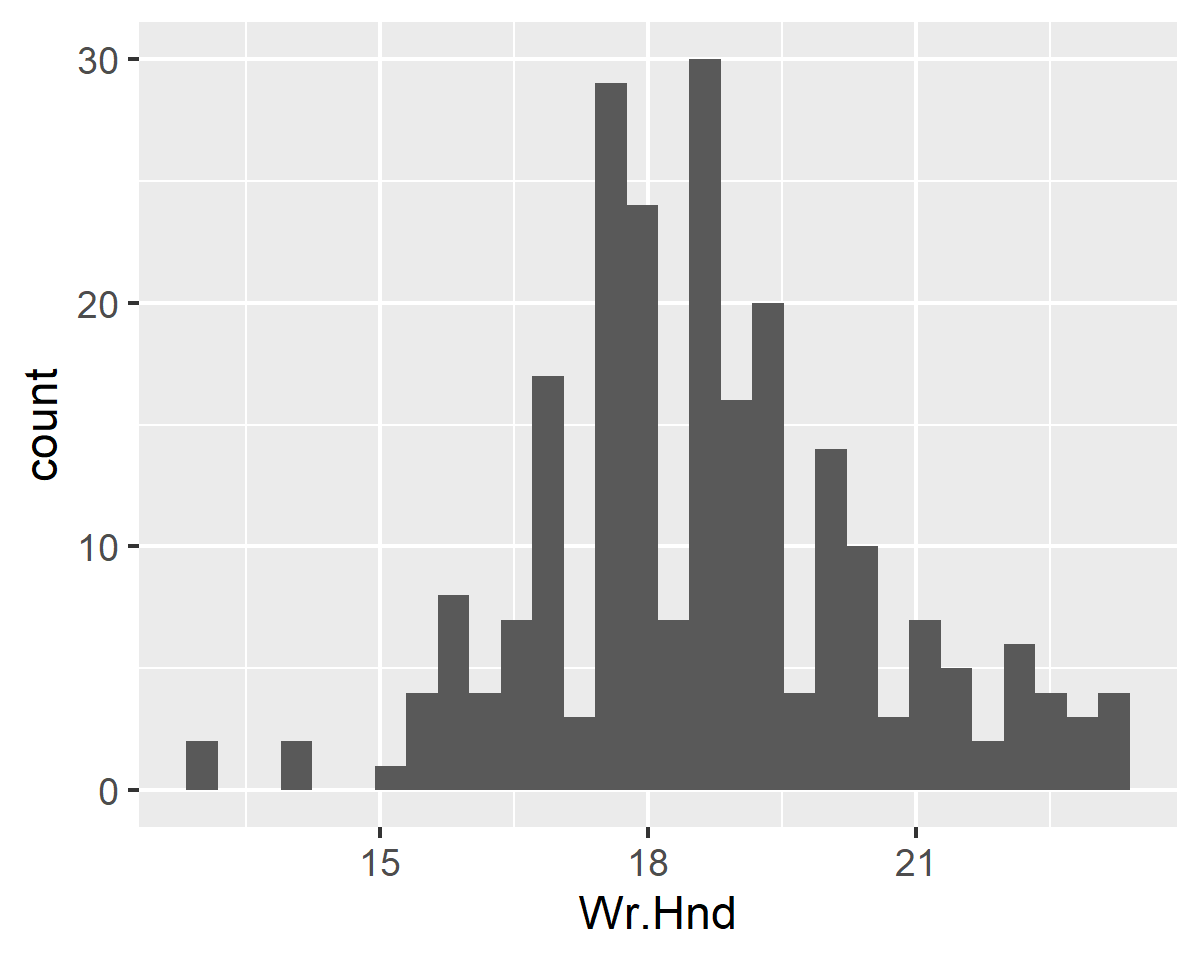
\includegraphics[width=0.5\linewidth]{03_Getting_started_with_a_data_analaysis_files/figure-latex/unnamed-chunk-62-1} 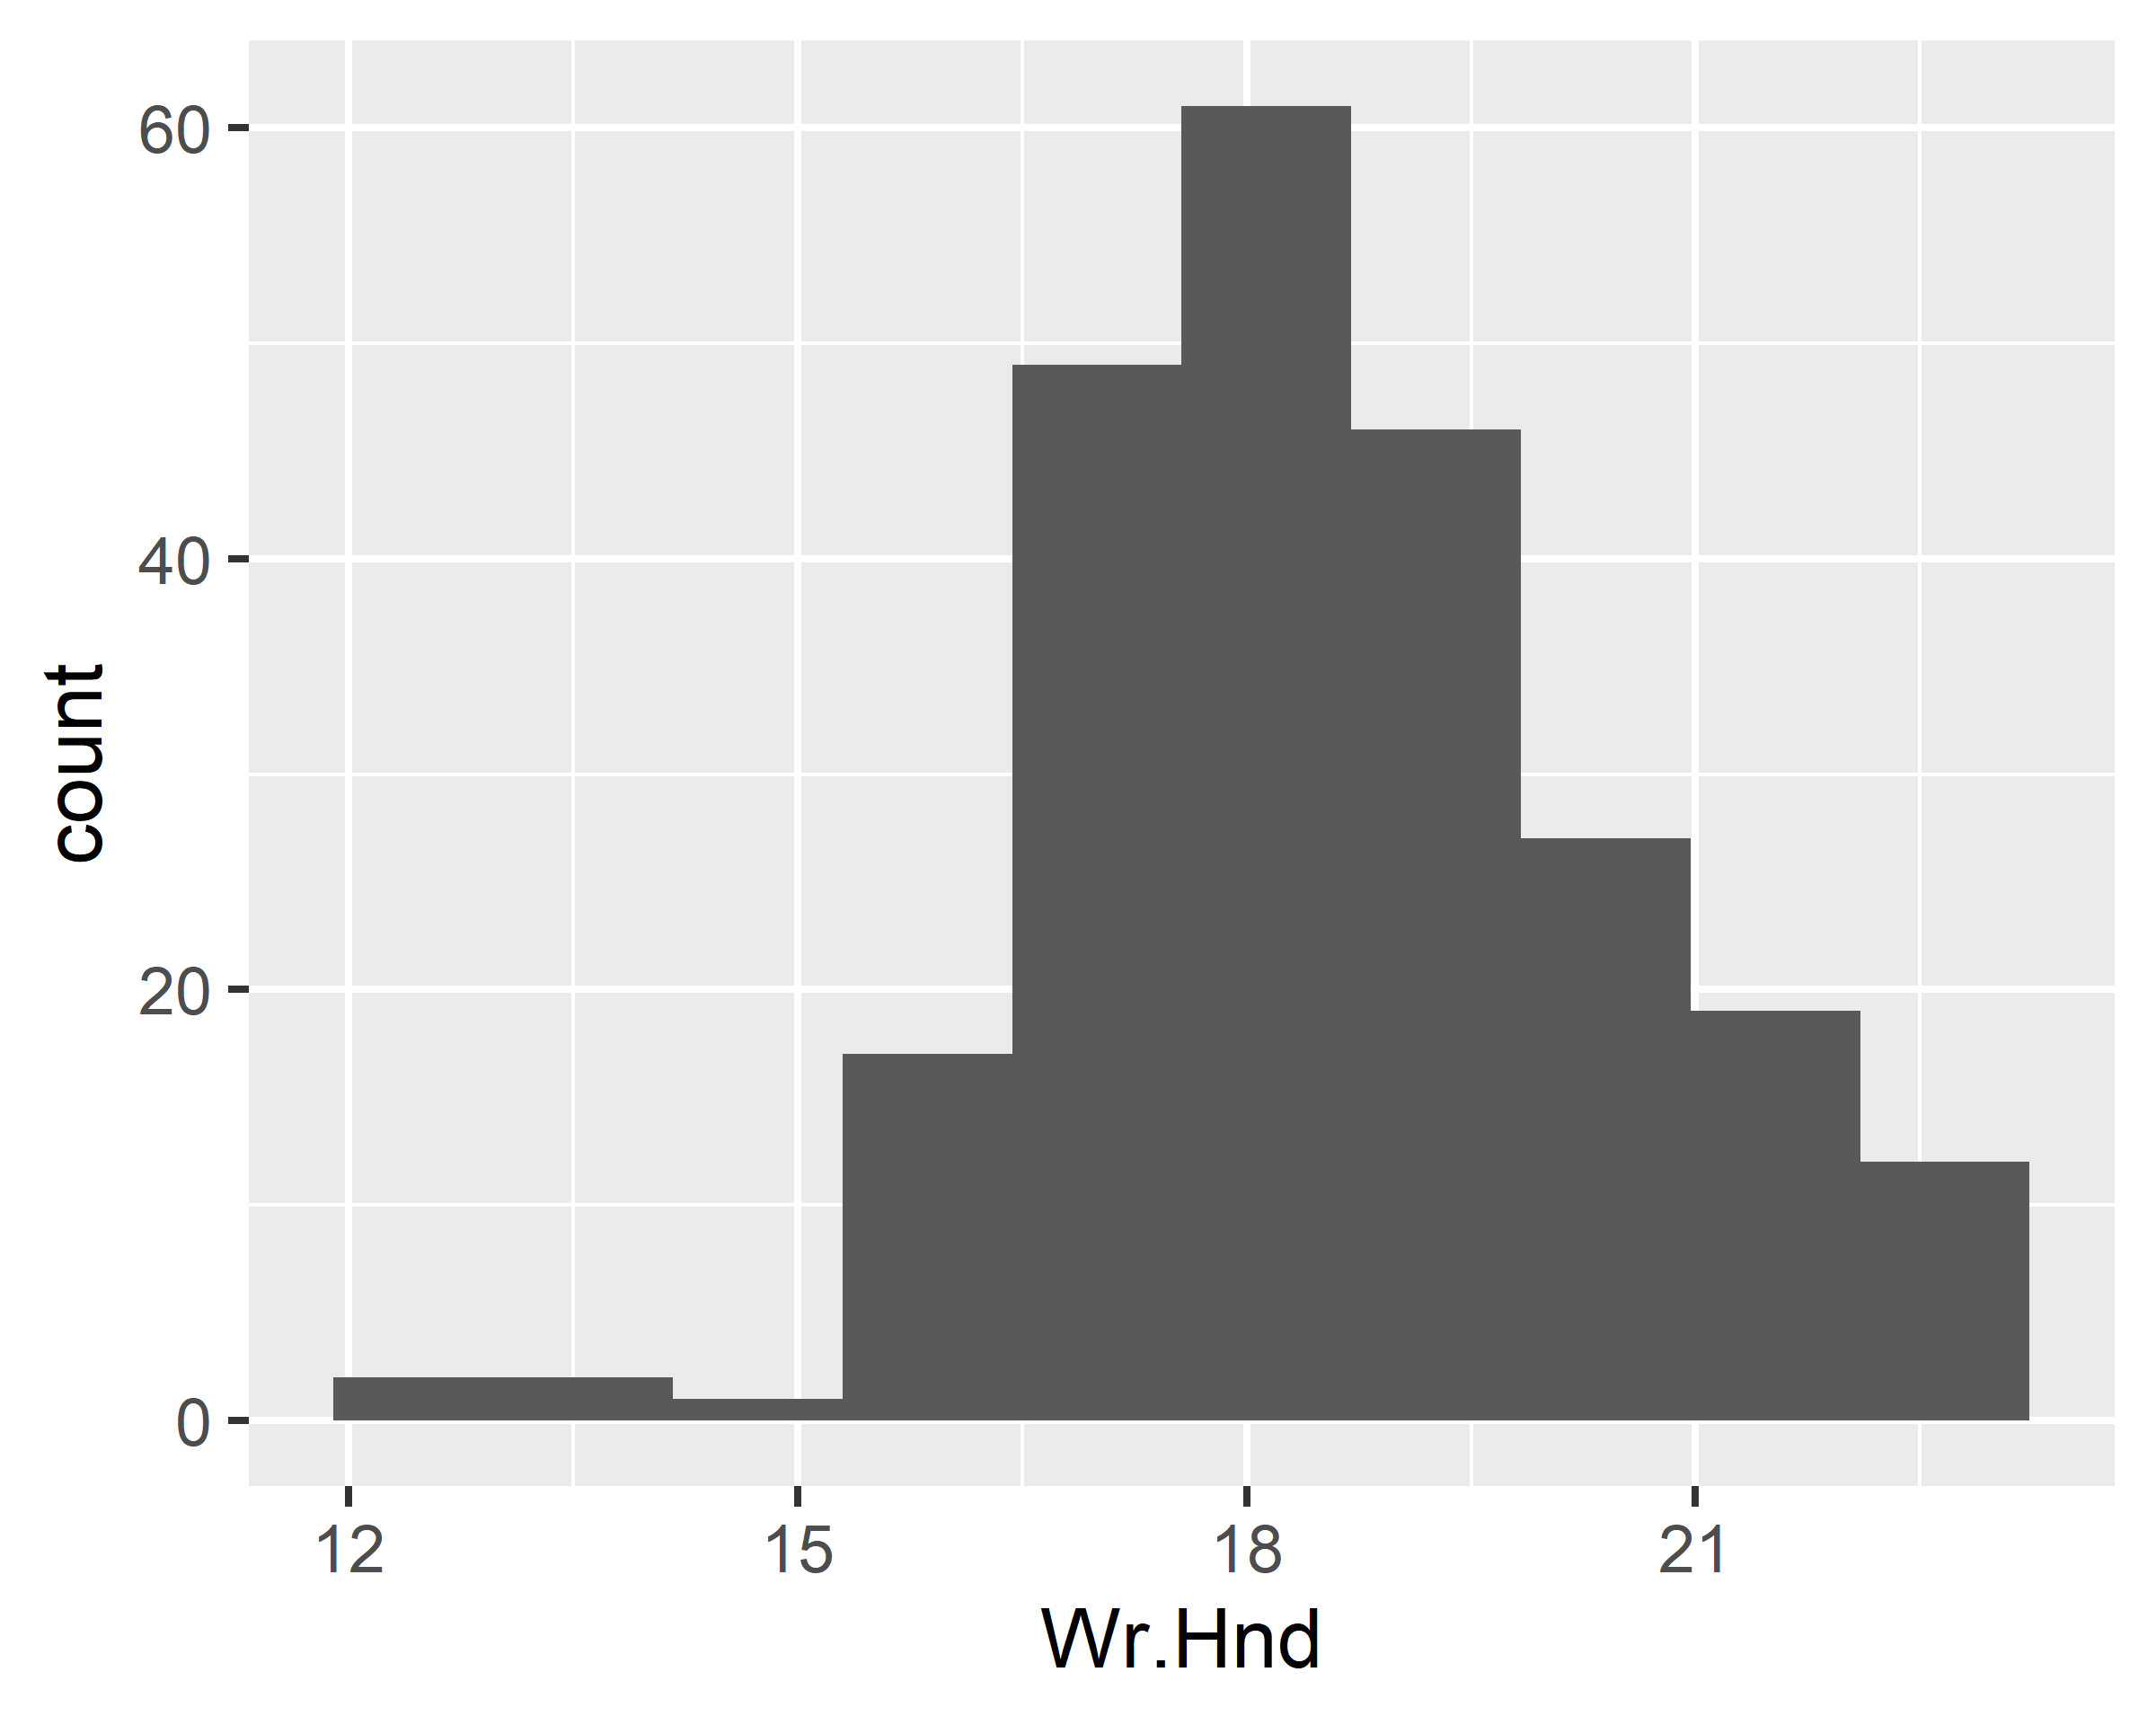
\includegraphics[width=0.5\linewidth]{03_Getting_started_with_a_data_analaysis_files/figure-latex/unnamed-chunk-62-2} \end{figure}

\begin{Shaded}
\begin{Highlighting}[]
\FunctionTok{ggplot}\NormalTok{(}\AttributeTok{data =}\NormalTok{ survey, }\AttributeTok{mapping =} \FunctionTok{aes}\NormalTok{(}\AttributeTok{x=}\NormalTok{Wr.Hnd)) }\SpecialCharTok{+} 
  \FunctionTok{geom\_histogram}\NormalTok{(}\AttributeTok{bins =} \DecValTok{10}\NormalTok{, }\AttributeTok{fill=}\StringTok{"lightblue"}\NormalTok{, }\AttributeTok{colour=}\StringTok{"blue"}\NormalTok{)}
\FunctionTok{ggplot}\NormalTok{(}\AttributeTok{data =}\NormalTok{ survey, }\AttributeTok{mapping =} \FunctionTok{aes}\NormalTok{(}\AttributeTok{x=}\NormalTok{Wr.Hnd)) }\SpecialCharTok{+} 
  \FunctionTok{geom\_histogram}\NormalTok{(}\AttributeTok{binwidth =} \DecValTok{1}\NormalTok{, }\AttributeTok{fill=}\StringTok{"lightblue"}\NormalTok{, }\AttributeTok{colour=}\StringTok{"blue"}\NormalTok{)}
\end{Highlighting}
\end{Shaded}

\begin{figure}
\includegraphics[width=0.5\linewidth]{03_Getting_started_with_a_data_analaysis_files/figure-latex/unnamed-chunk-63-1} \includegraphics[width=0.5\linewidth]{03_Getting_started_with_a_data_analaysis_files/figure-latex/unnamed-chunk-63-2} \end{figure}

\begin{Shaded}
\begin{Highlighting}[]
\FunctionTok{ggplot}\NormalTok{(}\AttributeTok{data =}\NormalTok{ survey, }\AttributeTok{mapping =} \FunctionTok{aes}\NormalTok{(}\AttributeTok{x=}\NormalTok{Wr.Hnd)) }\SpecialCharTok{+} 
  \FunctionTok{geom\_histogram}\NormalTok{(}\AttributeTok{binwidth =} \DecValTok{1}\NormalTok{, }\AttributeTok{fill=}\StringTok{"lightblue"}\NormalTok{, }\AttributeTok{colour=}\StringTok{"blue"}\NormalTok{) }\SpecialCharTok{+} 
  \FunctionTok{facet\_wrap}\NormalTok{(}\SpecialCharTok{\textasciitilde{}}\NormalTok{Sex)}
\FunctionTok{ggplot}\NormalTok{(}\AttributeTok{data =}\NormalTok{ survey[}\SpecialCharTok{!}\FunctionTok{is.na}\NormalTok{(survey}\SpecialCharTok{$}\NormalTok{Sex),], }\AttributeTok{mapping =} \FunctionTok{aes}\NormalTok{(}\AttributeTok{x=}\NormalTok{Wr.Hnd)) }\SpecialCharTok{+} 
  \FunctionTok{geom\_histogram}\NormalTok{(}\AttributeTok{binwidth =} \DecValTok{1}\NormalTok{, }\AttributeTok{fill=}\StringTok{"lightblue"}\NormalTok{, }\AttributeTok{colour=}\StringTok{"blue"}\NormalTok{) }\SpecialCharTok{+} 
  \FunctionTok{facet\_wrap}\NormalTok{(}\SpecialCharTok{\textasciitilde{}}\NormalTok{Sex)}
\end{Highlighting}
\end{Shaded}

\begin{figure}
\includegraphics[width=0.5\linewidth]{03_Getting_started_with_a_data_analaysis_files/figure-latex/unnamed-chunk-64-1} \includegraphics[width=0.5\linewidth]{03_Getting_started_with_a_data_analaysis_files/figure-latex/unnamed-chunk-64-2} \end{figure}

\begin{Shaded}
\begin{Highlighting}[]
\FunctionTok{ggplot}\NormalTok{(}\AttributeTok{data =}\NormalTok{ survey[}\SpecialCharTok{!}\FunctionTok{is.na}\NormalTok{(survey}\SpecialCharTok{$}\NormalTok{Sex),], }\AttributeTok{mapping =} \FunctionTok{aes}\NormalTok{(}\AttributeTok{x=}\NormalTok{Wr.Hnd)) }\SpecialCharTok{+} 
  \FunctionTok{geom\_histogram}\NormalTok{(}\AttributeTok{binwidth =} \DecValTok{1}\NormalTok{, }\AttributeTok{fill=}\StringTok{"lightblue"}\NormalTok{, }\AttributeTok{colour=}\StringTok{"blue"}\NormalTok{) }\SpecialCharTok{+} 
  \FunctionTok{facet\_wrap}\NormalTok{(}\SpecialCharTok{\textasciitilde{}}\NormalTok{Sex, }\AttributeTok{ncol=}\DecValTok{1}\NormalTok{)}
\end{Highlighting}
\end{Shaded}

\begin{figure}
\includegraphics[width=0.5\linewidth]{03_Getting_started_with_a_data_analaysis_files/figure-latex/unnamed-chunk-65-1} \end{figure}

\hypertarget{scatterplot-1}{%
\subsubsection{Scatterplot}\label{scatterplot-1}}

\begin{Shaded}
\begin{Highlighting}[]
\FunctionTok{ggplot}\NormalTok{(}\AttributeTok{data =}\NormalTok{ survey, }\AttributeTok{mapping =} \FunctionTok{aes}\NormalTok{(}\AttributeTok{x=}\NormalTok{Wr.Hnd, }\AttributeTok{y=}\NormalTok{Height)) }\SpecialCharTok{+} 
  \FunctionTok{geom\_point}\NormalTok{()}
\FunctionTok{ggplot}\NormalTok{(}\AttributeTok{data =}\NormalTok{ survey, }\AttributeTok{mapping =} \FunctionTok{aes}\NormalTok{(}\AttributeTok{x=}\NormalTok{Wr.Hnd, }\AttributeTok{y=}\NormalTok{Height, }\AttributeTok{color=}\NormalTok{Sex)) }\SpecialCharTok{+} 
  \FunctionTok{geom\_point}\NormalTok{()}
\end{Highlighting}
\end{Shaded}

\begin{figure}
\includegraphics[width=0.5\linewidth]{03_Getting_started_with_a_data_analaysis_files/figure-latex/unnamed-chunk-66-1} \includegraphics[width=0.5\linewidth]{03_Getting_started_with_a_data_analaysis_files/figure-latex/unnamed-chunk-66-2} \end{figure}

\begin{Shaded}
\begin{Highlighting}[]
\FunctionTok{ggplot}\NormalTok{(}\AttributeTok{data =}\NormalTok{ survey, }\AttributeTok{mapping =} \FunctionTok{aes}\NormalTok{(}\AttributeTok{x=}\NormalTok{Wr.Hnd, }\AttributeTok{y=}\NormalTok{Height, }\AttributeTok{color=}\NormalTok{Sex)) }\SpecialCharTok{+} 
  \FunctionTok{geom\_point}\NormalTok{() }\SpecialCharTok{+} \FunctionTok{scale\_color\_discrete}\NormalTok{(}\AttributeTok{na.translate=}\NormalTok{F)}
\FunctionTok{ggplot}\NormalTok{(}\AttributeTok{data =}\NormalTok{ survey, }\AttributeTok{mapping =} \FunctionTok{aes}\NormalTok{(}\AttributeTok{x=}\NormalTok{Wr.Hnd, }\AttributeTok{y=}\NormalTok{Height, }\AttributeTok{color=}\NormalTok{Sex)) }\SpecialCharTok{+} 
  \FunctionTok{geom\_point}\NormalTok{() }\SpecialCharTok{+} \FunctionTok{scale\_color\_discrete}\NormalTok{(}\AttributeTok{na.translate=}\NormalTok{F) }\SpecialCharTok{+} 
  \FunctionTok{geom\_smooth}\NormalTok{(}\AttributeTok{se =}\NormalTok{ F, }\AttributeTok{method =}\NormalTok{ lm)}
\end{Highlighting}
\end{Shaded}

\begin{figure}
\includegraphics[width=0.5\linewidth]{03_Getting_started_with_a_data_analaysis_files/figure-latex/unnamed-chunk-67-1} \includegraphics[width=0.5\linewidth]{03_Getting_started_with_a_data_analaysis_files/figure-latex/unnamed-chunk-67-2} \end{figure}

\hypertarget{box-plot-1}{%
\subsubsection{Box plot}\label{box-plot-1}}

\begin{Shaded}
\begin{Highlighting}[]
\FunctionTok{ggplot}\NormalTok{(}\AttributeTok{data =}\NormalTok{ survey, }\AttributeTok{mapping =} \FunctionTok{aes}\NormalTok{(}\AttributeTok{x=}\NormalTok{Sex, }\AttributeTok{y=}\NormalTok{Wr.Hnd)) }\SpecialCharTok{+} 
  \FunctionTok{geom\_boxplot}\NormalTok{()}
\FunctionTok{ggplot}\NormalTok{(}\AttributeTok{data =}\NormalTok{ survey, }\AttributeTok{mapping =} \FunctionTok{aes}\NormalTok{(}\AttributeTok{x=}\NormalTok{Sex, }\AttributeTok{y=}\NormalTok{Wr.Hnd)) }\SpecialCharTok{+} 
  \FunctionTok{geom\_boxplot}\NormalTok{() }\SpecialCharTok{+} \FunctionTok{scale\_x\_discrete}\NormalTok{(}\AttributeTok{na.translate=}\NormalTok{F)}
\end{Highlighting}
\end{Shaded}

\begin{figure}
\includegraphics[width=0.5\linewidth]{03_Getting_started_with_a_data_analaysis_files/figure-latex/unnamed-chunk-68-1} \includegraphics[width=0.5\linewidth]{03_Getting_started_with_a_data_analaysis_files/figure-latex/unnamed-chunk-68-2} \end{figure}

\begin{Shaded}
\begin{Highlighting}[]
\FunctionTok{ggplot}\NormalTok{(}\AttributeTok{data =}\NormalTok{ survey, }\AttributeTok{mapping =} \FunctionTok{aes}\NormalTok{(}\AttributeTok{x=}\NormalTok{Sex, }\AttributeTok{y=}\NormalTok{Wr.Hnd, }\AttributeTok{fill=}\NormalTok{Sex)) }\SpecialCharTok{+} 
  \FunctionTok{geom\_boxplot}\NormalTok{() }\SpecialCharTok{+} \FunctionTok{scale\_x\_discrete}\NormalTok{(}\AttributeTok{na.translate=}\NormalTok{F) }

\FunctionTok{ggplot}\NormalTok{(}\AttributeTok{data =}\NormalTok{ survey, }\AttributeTok{mapping =} \FunctionTok{aes}\NormalTok{(}\AttributeTok{x=}\NormalTok{Sex, }\AttributeTok{y=}\NormalTok{Wr.Hnd, }\AttributeTok{fill=}\NormalTok{Sex)) }\SpecialCharTok{+} 
  \FunctionTok{geom\_boxplot}\NormalTok{() }\SpecialCharTok{+} \FunctionTok{scale\_x\_discrete}\NormalTok{(}\AttributeTok{na.translate=}\NormalTok{F) }\SpecialCharTok{+} 
  \FunctionTok{scale\_fill\_discrete}\NormalTok{(}\AttributeTok{guide=}\NormalTok{F) }
\end{Highlighting}
\end{Shaded}

\begin{figure}
\includegraphics[width=0.5\linewidth]{03_Getting_started_with_a_data_analaysis_files/figure-latex/unnamed-chunk-69-1} \includegraphics[width=0.5\linewidth]{03_Getting_started_with_a_data_analaysis_files/figure-latex/unnamed-chunk-69-2} \end{figure}

\hypertarget{stripchart}{%
\subsubsection{Stripchart}\label{stripchart}}

\begin{Shaded}
\begin{Highlighting}[]
\FunctionTok{ggplot}\NormalTok{(}\AttributeTok{data =}\NormalTok{ survey, }\AttributeTok{mapping =} \FunctionTok{aes}\NormalTok{(}\AttributeTok{x=}\DecValTok{1}\NormalTok{, }\AttributeTok{y=}\NormalTok{Wr.Hnd)) }\SpecialCharTok{+} 
  \FunctionTok{geom\_jitter}\NormalTok{() }\SpecialCharTok{+} \FunctionTok{scale\_x\_discrete}\NormalTok{(}\AttributeTok{na.translate=}\NormalTok{F) }
\FunctionTok{ggplot}\NormalTok{(}\AttributeTok{data =}\NormalTok{ survey, }\AttributeTok{mapping =} \FunctionTok{aes}\NormalTok{(}\AttributeTok{x=}\NormalTok{Sex, }\AttributeTok{y=}\NormalTok{Wr.Hnd)) }\SpecialCharTok{+} 
  \FunctionTok{geom\_jitter}\NormalTok{() }\SpecialCharTok{+} \FunctionTok{scale\_x\_discrete}\NormalTok{(}\AttributeTok{na.translate=}\NormalTok{F)}
\end{Highlighting}
\end{Shaded}

\begin{figure}
\includegraphics[width=0.5\linewidth]{03_Getting_started_with_a_data_analaysis_files/figure-latex/unnamed-chunk-71-1} \includegraphics[width=0.5\linewidth]{03_Getting_started_with_a_data_analaysis_files/figure-latex/unnamed-chunk-71-2} \end{figure}

\begin{Shaded}
\begin{Highlighting}[]
\FunctionTok{ggplot}\NormalTok{(}\AttributeTok{data =}\NormalTok{ survey, }\AttributeTok{mapping =} \FunctionTok{aes}\NormalTok{(}\AttributeTok{x=}\NormalTok{Sex, }\AttributeTok{y=}\NormalTok{Wr.Hnd)) }\SpecialCharTok{+} 
  \FunctionTok{geom\_jitter}\NormalTok{(}\AttributeTok{width =} \FloatTok{0.1}\NormalTok{) }\SpecialCharTok{+} \FunctionTok{scale\_x\_discrete}\NormalTok{(}\AttributeTok{na.translate=}\NormalTok{F) }
\FunctionTok{ggplot}\NormalTok{(}\AttributeTok{data =}\NormalTok{ survey, }\AttributeTok{mapping =} \FunctionTok{aes}\NormalTok{(}\AttributeTok{x=}\NormalTok{Sex, }\AttributeTok{y=}\NormalTok{Wr.Hnd)) }\SpecialCharTok{+} 
  \FunctionTok{geom\_jitter}\NormalTok{(}\AttributeTok{width =} \FloatTok{0.1}\NormalTok{, }\AttributeTok{alpha=}\FloatTok{0.5}\NormalTok{, }\AttributeTok{color=}\StringTok{"red"}\NormalTok{) }\SpecialCharTok{+} 
  \FunctionTok{scale\_x\_discrete}\NormalTok{(}\AttributeTok{na.translate=}\NormalTok{F) }\SpecialCharTok{+}
  \FunctionTok{geom\_boxplot}\NormalTok{(}\AttributeTok{alpha=}\FloatTok{0.5}\NormalTok{)}
\end{Highlighting}
\end{Shaded}

\begin{figure}
\includegraphics[width=0.5\linewidth]{03_Getting_started_with_a_data_analaysis_files/figure-latex/unnamed-chunk-72-1} \includegraphics[width=0.5\linewidth]{03_Getting_started_with_a_data_analaysis_files/figure-latex/unnamed-chunk-72-2} \end{figure}

\hypertarget{appendix-appendix}{%
\appendix}


\hypertarget{recaps-in-1-minutes-or-less}{%
\chapter{Recaps in 1 minutes or less}\label{recaps-in-1-minutes-or-less}}

\hypertarget{possibilities-of-using-r}{%
\section{Possibilities of using R}\label{possibilities-of-using-r}}

\begin{itemize}
\item
  Console: type a command and hit Enter

  \begin{itemize}
  \tightlist
  \item
    \emph{Base R} Console
  \item
    \emph{RGui} Console on Windows
  \item
    \emph{RStudio} Console
  \end{itemize}
\item
  Script: edit a text files and hit Ctrl+R or Ctrl+Enter

  \begin{itemize}
  \tightlist
  \item
    \emph{RGui} Script Window (Ctrl+R)
  \item
    \emph{RStudio} Source Pane (Ctrl+Enter)
  \end{itemize}
\item
  Point and Click

  \begin{itemize}
  \tightlist
  \item
    \emph{R Commander}
  \item
    \emph{jamovi}, \emph{JASP} etc.
  \end{itemize}
\end{itemize}

\hypertarget{console-features-1}{%
\section{Console features}\label{console-features-1}}

\begin{itemize}
\tightlist
\item
  history of command: Up/Down arrows
\item
  autocompletion: TAB
\item
  continuation prompt: Esc
\end{itemize}

\hypertarget{advantages-of-script-editor-in-rstudio}{%
\section{Advantages of Script editor in RStudio}\label{advantages-of-script-editor-in-rstudio}}

\begin{itemize}
\tightlist
\item
  multi-line editor
\item
  full-featured text editor: e.g.~row numbering, syntax highlighting
\item
  autocompletion of filenames, function names, arguments and objects
\item
  cross-platform interface to R
\item
  surrounded by integrated graphical environment (workspace, files, plots, help, etc.)
\end{itemize}

\hypertarget{useful-keyboard-shortcuts-in-rstudio}{%
\section{Useful keyboard shortcuts in RStudio}\label{useful-keyboard-shortcuts-in-rstudio}}

\begin{itemize}
\tightlist
\item
  Ctrl+Enter: Run commands
\item
  Clipboard Operations (Cut, Copy, Paste Operations): Ctrl+X, Ctrl+C, Ctrl+V
\item
  Ctrl++, Ctrl+-: Zoom in/out
\item
  Ctrl+Shift+C: Comment lines/uncomment lines
\item
  Ctrl+F: Find and replace text within script editor
\item
  Ctrl+S: Save the script file
\item
  Alt+-: Write assignment operator
\item
  Ctrl+Shift+F10: Restart R session
\end{itemize}

\hypertarget{base-types-in-r}{%
\section{Base types in R}\label{base-types-in-r}}

\begin{itemize}
\tightlist
\item
  character (or string): \texttt{"apple\ juice"}
\item
  integer (whole numbers): \texttt{12L}
\item
  double (real numbers, decimal numbers): \texttt{12}, \texttt{12.4}
\item
  logical (true false type things): \texttt{TRUE}, \texttt{FALSE}
\end{itemize}

\hypertarget{data-structures-1}{%
\section{Data structures}\label{data-structures-1}}

\begin{itemize}
\tightlist
\item
  \emph{Vector}: one-dimensional, homogeneous
\item
  \emph{Matrix}: two-dimensional, homogeneous
\item
  \emph{Array}: two or more dimensional, homogeneous
\item
  \emph{List}: one-dimensional, heterogeneous
\item
  \emph{Factor}: integer vector with levels, which is a character vector
\item
  \emph{Data frame}: two-dimensional, heterogeneous
\end{itemize}

\begin{longtable}[]{@{}ccc@{}}
\caption{Data structures}\tabularnewline
\toprule
Dimension & Homogenous & Heterogeneous\tabularnewline
\midrule
\endfirsthead
\toprule
Dimension & Homogenous & Heterogeneous\tabularnewline
\midrule
\endhead
1D & Vector, Factor & List\tabularnewline
2D & Matrix & Data frame\tabularnewline
nD & Array &\tabularnewline
\bottomrule
\end{longtable}

\hypertarget{operators-1}{%
\section{Operators}\label{operators-1}}

\begin{longtable}[]{@{}lll@{}}
\caption{R operators in order of precedence from highest to lowest}\tabularnewline
\toprule
Operator & Description & Example\tabularnewline
\midrule
\endfirsthead
\toprule
Operator & Description & Example\tabularnewline
\midrule
\endhead
\texttt{::} & access & \texttt{MASS::survey}\tabularnewline
\texttt{\$} & component & \texttt{my.s\$Sex}\tabularnewline
\texttt{{[}} \texttt{{[}{[}} & indexing & \texttt{my.s\$Height{[}c(2,\ 45){]}}\tabularnewline
\texttt{\^{}} \texttt{**} & exponentiation & \texttt{2\^{}3}\tabularnewline
\texttt{-} \texttt{+} & unary minus, unary plus & \texttt{-2}\tabularnewline
\texttt{:} & sequence operator & \texttt{1:10}\tabularnewline
\texttt{\%any\%} e.g.~\texttt{\%\%} \texttt{\%/\%} \texttt{\%in\%} & special operators & \texttt{12\%\%3}\tabularnewline
\texttt{*} \texttt{/} & multiplication, division & \texttt{12*3}\tabularnewline
\texttt{+} \texttt{-} & addition, subtraction & \texttt{2.3\ +\ 2}\tabularnewline
\texttt{\textless{}} \texttt{\textgreater{}} \texttt{\textless{}=} \texttt{\textgreater{}=} \texttt{==} \texttt{!=} & comparisions & \texttt{2\textless{}=3}\tabularnewline
\texttt{!} & logical NOT & \texttt{!TRUE}\tabularnewline
\texttt{\&} & logical AND & \texttt{TRUE\ \&\ FALSE}\tabularnewline
\texttt{\textbar{}} & logical OR & \texttt{TRUE\ \textbar{}\ FALSE}\tabularnewline
\texttt{\textless{}-} & assignment & \texttt{col\ \textless{}-\ 12}\tabularnewline
\bottomrule
\end{longtable}

R language provides following types of operators:

\begin{itemize}
\tightlist
\item
  Arithmetic Operators: \texttt{\^{}} \texttt{**}, \texttt{-} (unary), \texttt{+} (unary), \texttt{\%\%}, \texttt{\%/\%}, \texttt{*}, \texttt{/}, \texttt{-} (binary), \texttt{+} (binary)
\item
  Relational Operators: \texttt{\textless{}}, \texttt{\textgreater{}}, \texttt{\textless{}=}, \texttt{\textgreater{}=}, \texttt{==}, \texttt{!=}, \texttt{\%in\%}
\item
  Logical Operators: \texttt{!}, \texttt{\&}, \texttt{\textbar{}}
\item
  Assignment Operators: \texttt{\textless{}-}
\item
  Miscellaneous Operators: \texttt{::}, \texttt{\$}, \texttt{{[}}, \texttt{{[}{[}}, \texttt{:}, \texttt{?}
\end{itemize}

\hypertarget{maths-functions}{%
\section{Maths functions}\label{maths-functions}}

\begin{longtable}[]{@{}lll@{}}
\caption{\label{tab:matfuggvenyek}Mathematical functions}\tabularnewline
\toprule
Function & Description & Example\tabularnewline
\midrule
\endfirsthead
\toprule
Function & Description & Example\tabularnewline
\midrule
\endhead
{abs(x)} & Takes the absolute value of x & {abs(-1)}\tabularnewline
{sign(x)} & The signs of \texttt{x} & {sign(pi)}\tabularnewline
{sqrt(x)} & Returns the square root of x & {sqrt(9+16)}\tabularnewline
{exp(x)} & Returns the exponential of x & {exp(1)}\tabularnewline
{log(x,base=exp(1))} & Takes the logarithm of x with base y; if base is not specified, returns the natural logarithm & {log(exp(3));log(8,10)}\tabularnewline
{log10(x);log2(x)} & Takes the logarithm of x with base 10 or 2 & {log10(1000);log2(256)}\tabularnewline
{cos(x);sin(x);tan(x)} & Trigonometric functions & {cos(pi);sin(0);tan(0)}\tabularnewline
{round(x,digits=0)} & Rounds a numeric input to a specified number of decimal places & {round(c(1.5,-1.5))}\tabularnewline
{floor(x)} & Rounds a numeric input down to the next lower integer & {floor(c(1.5,-1.5))}\tabularnewline
{ceiling(x)} & Rounds a numeric input up to the next higher integer & {ceiling(c(1.5,-1.5))}\tabularnewline
{trunc(x)} & Truncates (i.e.~cuts off) the decimal places of a numeric input & {trunc(c(1.5,-1.5))}\tabularnewline
\bottomrule
\end{longtable}

\hypertarget{string-functions}{%
\section{String functions}\label{string-functions}}

\begin{longtable}[]{@{}lll@{}}
\toprule
\begin{minipage}[b]{(\columnwidth - 2\tabcolsep) * \real{0.32}}\raggedright
Function\strut
\end{minipage} & \begin{minipage}[b]{(\columnwidth - 2\tabcolsep) * \real{0.41}}\raggedright
Description\strut
\end{minipage} & \begin{minipage}[b]{(\columnwidth - 2\tabcolsep) * \real{0.27}}\raggedright
Example\strut
\end{minipage}\tabularnewline
\midrule
\endhead
\begin{minipage}[t]{(\columnwidth - 2\tabcolsep) * \real{0.32}}\raggedright
\texttt{paste();paste0(sep="")}\strut
\end{minipage} & \begin{minipage}[t]{(\columnwidth - 2\tabcolsep) * \real{0.41}}\raggedright
Concatenate strings\strut
\end{minipage} & \begin{minipage}[t]{(\columnwidth - 2\tabcolsep) * \real{0.27}}\raggedright
\texttt{paste(\textquotesingle{}a\textquotesingle{},\textquotesingle{}b\textquotesingle{},sep=\textquotesingle{}=\textquotesingle{})}\strut
\end{minipage}\tabularnewline
\begin{minipage}[t]{(\columnwidth - 2\tabcolsep) * \real{0.32}}\raggedright
\texttt{nchar(x)}\strut
\end{minipage} & \begin{minipage}[t]{(\columnwidth - 2\tabcolsep) * \real{0.41}}\raggedright
Count the number of characters\strut
\end{minipage} & \begin{minipage}[t]{(\columnwidth - 2\tabcolsep) * \real{0.27}}\raggedright
\texttt{nchar(\textquotesingle{}alma\textquotesingle{})}\strut
\end{minipage}\tabularnewline
\begin{minipage}[t]{(\columnwidth - 2\tabcolsep) * \real{0.32}}\raggedright
\texttt{substr(x,start,stop)}\strut
\end{minipage} & \begin{minipage}[t]{(\columnwidth - 2\tabcolsep) * \real{0.41}}\raggedright
Substrings of a character vector\strut
\end{minipage} & \begin{minipage}[t]{(\columnwidth - 2\tabcolsep) * \real{0.27}}\raggedright
\texttt{substr(\textquotesingle{}alma\textquotesingle{},\ 3,\ 5)}\strut
\end{minipage}\tabularnewline
\begin{minipage}[t]{(\columnwidth - 2\tabcolsep) * \real{0.32}}\raggedright
\texttt{tolower(x)}\strut
\end{minipage} & \begin{minipage}[t]{(\columnwidth - 2\tabcolsep) * \real{0.41}}\raggedright
Convert to lower-case\strut
\end{minipage} & \begin{minipage}[t]{(\columnwidth - 2\tabcolsep) * \real{0.27}}\raggedright
\texttt{tolower(\textquotesingle{}Kiss\ Géza\textquotesingle{})}\strut
\end{minipage}\tabularnewline
\begin{minipage}[t]{(\columnwidth - 2\tabcolsep) * \real{0.32}}\raggedright
\texttt{toupper(x)}\strut
\end{minipage} & \begin{minipage}[t]{(\columnwidth - 2\tabcolsep) * \real{0.41}}\raggedright
Convert to upper-case\strut
\end{minipage} & \begin{minipage}[t]{(\columnwidth - 2\tabcolsep) * \real{0.27}}\raggedright
\texttt{toupper(\textquotesingle{}Kiss\ Géza\textquotesingle{})}\strut
\end{minipage}\tabularnewline
\begin{minipage}[t]{(\columnwidth - 2\tabcolsep) * \real{0.32}}\raggedright
\texttt{chartr(old,new,x)}\strut
\end{minipage} & \begin{minipage}[t]{(\columnwidth - 2\tabcolsep) * \real{0.41}}\raggedright
Translates characters\strut
\end{minipage} & \begin{minipage}[t]{(\columnwidth - 2\tabcolsep) * \real{0.27}}\raggedright
\texttt{chartr(\textquotesingle{}it\textquotesingle{},\textquotesingle{}ál\textquotesingle{},\textquotesingle{}titik\textquotesingle{})}\strut
\end{minipage}\tabularnewline
\begin{minipage}[t]{(\columnwidth - 2\tabcolsep) * \real{0.32}}\raggedright
\texttt{cat(sep="\ ")}\strut
\end{minipage} & \begin{minipage}[t]{(\columnwidth - 2\tabcolsep) * \real{0.41}}\raggedright
Concatenate and print\strut
\end{minipage} & \begin{minipage}[t]{(\columnwidth - 2\tabcolsep) * \real{0.27}}\raggedright
\texttt{cat(\textquotesingle{}alma\textquotesingle{},\textquotesingle{}fa\textbackslash{}n\textquotesingle{},sep=\textquotesingle{}\textquotesingle{})}\strut
\end{minipage}\tabularnewline
\begin{minipage}[t]{(\columnwidth - 2\tabcolsep) * \real{0.32}}\raggedright
\texttt{grep();grepl();regexpr()}\strut
\end{minipage} & \begin{minipage}[t]{(\columnwidth - 2\tabcolsep) * \real{0.41}}\raggedright
Pattern matching\strut
\end{minipage} & \begin{minipage}[t]{(\columnwidth - 2\tabcolsep) * \real{0.27}}\raggedright
\texttt{grepl(pattern=\textquotesingle{}lm\textquotesingle{},x=\textquotesingle{}alma\textquotesingle{})}\strut
\end{minipage}\tabularnewline
\begin{minipage}[t]{(\columnwidth - 2\tabcolsep) * \real{0.32}}\raggedright
\texttt{sub();gsub()}\strut
\end{minipage} & \begin{minipage}[t]{(\columnwidth - 2\tabcolsep) * \real{0.41}}\raggedright
Pattern matching and replacement\strut
\end{minipage} & \begin{minipage}[t]{(\columnwidth - 2\tabcolsep) * \real{0.27}}\raggedright
\texttt{gsub(\textquotesingle{}lm\textquotesingle{},repl=\textquotesingle{}nyj\textquotesingle{},x=\textquotesingle{}alma\textquotesingle{})}\strut
\end{minipage}\tabularnewline
\bottomrule
\end{longtable}

\hypertarget{base-r-statistical-functions}{%
\section{Base R Statistical Functions}\label{base-r-statistical-functions}}

\begin{longtable}[]{@{}llll@{}}
\caption{\label{tab:statfuggvenyek2}Base R Statistical Functions}\tabularnewline
\toprule
Function & Description & Example & Value of Example\tabularnewline
\midrule
\endfirsthead
\toprule
Function & Description & Example & Value of Example\tabularnewline
\midrule
\endhead
{max(x)} & The largest value of \texttt{x} & {max(1:10)} & {10}\tabularnewline
{min(x)} & The smallest value of \texttt{x} & {min(11:20)} & {11}\tabularnewline
{sum(x)} & The sum of all the values of \texttt{x} & {sum(1:5)} & {15}\tabularnewline
{prod(x)} & The product of all the values of \texttt{x} & {prod(1:5)} & {120}\tabularnewline
{mean(x)} & Mean of \texttt{x} & {mean(1:10)} & {5.5}\tabularnewline
{median(x)} & Median of \texttt{x} & {median(1:10)} & {5.5}\tabularnewline
{range(x)} & The minimum and the maximum & {range(1:10)} & {1 10}\tabularnewline
{sd(x)} & Standard deviation of x & {sd(1:10)} & {3.03}\tabularnewline
{var(x)} & Variance of \texttt{x} & {var(1:10)} & {9.17}\tabularnewline
{cor(x,y)} & Correlation between \texttt{x} and \texttt{y} & {cor(1:10,11:20)} & {1}\tabularnewline
\bottomrule
\end{longtable}

\hypertarget{regular-sequences}{%
\section{Regular sequences}\label{regular-sequences}}

\begin{longtable}[]{@{}llll@{}}
\toprule
\begin{minipage}[b]{(\columnwidth - 3\tabcolsep) * \real{0.21}}\raggedright
Function\strut
\end{minipage} & \begin{minipage}[b]{(\columnwidth - 3\tabcolsep) * \real{0.42}}\raggedright
Description\strut
\end{minipage} & \begin{minipage}[b]{(\columnwidth - 3\tabcolsep) * \real{0.18}}\raggedright
Example\strut
\end{minipage} & \begin{minipage}[b]{(\columnwidth - 3\tabcolsep) * \real{0.19}}\raggedright
Value of Example\strut
\end{minipage}\tabularnewline
\midrule
\endhead
\begin{minipage}[t]{(\columnwidth - 3\tabcolsep) * \real{0.21}}\raggedright
\texttt{from:to}\strut
\end{minipage} & \begin{minipage}[t]{(\columnwidth - 3\tabcolsep) * \real{0.42}}\raggedright
generates a sequence from \texttt{from=} to \texttt{to=} in steps of 1 or -1\strut
\end{minipage} & \begin{minipage}[t]{(\columnwidth - 3\tabcolsep) * \real{0.18}}\raggedright
\texttt{1:5}\strut
\end{minipage} & \begin{minipage}[t]{(\columnwidth - 3\tabcolsep) * \real{0.19}}\raggedright
\texttt{1\ 2\ 3\ 4\ 5}\strut
\end{minipage}\tabularnewline
\begin{minipage}[t]{(\columnwidth - 3\tabcolsep) * \real{0.21}}\raggedright
\texttt{seq(from,\ to,\ by,\ length.out)}\strut
\end{minipage} & \begin{minipage}[t]{(\columnwidth - 3\tabcolsep) * \real{0.42}}\raggedright
generate regular sequences\strut
\end{minipage} & \begin{minipage}[t]{(\columnwidth - 3\tabcolsep) * \real{0.18}}\raggedright
\texttt{seq(from=2,\ to=10,\ by=2)}\strut
\end{minipage} & \begin{minipage}[t]{(\columnwidth - 3\tabcolsep) * \real{0.19}}\raggedright
\texttt{2\ \ 4\ \ 6\ \ 8\ 10}\strut
\end{minipage}\tabularnewline
\begin{minipage}[t]{(\columnwidth - 3\tabcolsep) * \real{0.21}}\raggedright
\texttt{rep(x,\ times,\ each)}\strut
\end{minipage} & \begin{minipage}[t]{(\columnwidth - 3\tabcolsep) * \real{0.42}}\raggedright
replicate elements of vectors\strut
\end{minipage} & \begin{minipage}[t]{(\columnwidth - 3\tabcolsep) * \real{0.18}}\raggedright
\texttt{rep(x=0,\ times=3)}\strut
\end{minipage} & \begin{minipage}[t]{(\columnwidth - 3\tabcolsep) * \real{0.19}}\raggedright
\texttt{0\ 0\ 0}\strut
\end{minipage}\tabularnewline
\begin{minipage}[t]{(\columnwidth - 3\tabcolsep) * \real{0.21}}\raggedright
\texttt{paste(sep,\ collapse)}\strut
\end{minipage} & \begin{minipage}[t]{(\columnwidth - 3\tabcolsep) * \real{0.42}}\raggedright
concatenate vectors\strut
\end{minipage} & \begin{minipage}[t]{(\columnwidth - 3\tabcolsep) * \real{0.18}}\raggedright
\texttt{paste("No",\ 1:3,\ sep="\_")}\strut
\end{minipage} & \begin{minipage}[t]{(\columnwidth - 3\tabcolsep) * \real{0.19}}\raggedright
\texttt{"No\_1"\ "No\_2"\ "No\_3"}\strut
\end{minipage}\tabularnewline
\bottomrule
\end{longtable}

\hypertarget{subsetting-1}{%
\section{Subsetting}\label{subsetting-1}}

\begin{longtable}[]{@{}ll@{}}
\toprule
\begin{minipage}[b]{(\columnwidth - 1\tabcolsep) * \real{0.42}}\raggedright
Data structure\strut
\end{minipage} & \begin{minipage}[b]{(\columnwidth - 1\tabcolsep) * \real{0.56}}\raggedright
Example\strut
\end{minipage}\tabularnewline
\midrule
\endhead
\begin{minipage}[t]{(\columnwidth - 1\tabcolsep) * \real{0.42}}\raggedright
\begin{itemize}
\tightlist
\item
  Vector
\item
  Factor
\item
  List
\item
  Data frame
\end{itemize}\strut
\end{minipage} & \begin{minipage}[t]{(\columnwidth - 1\tabcolsep) * \real{0.56}}\raggedright
\begin{itemize}
\tightlist
\item
  \texttt{x{[}3{]}}
\item
  \texttt{x{[}1:3{]}}
\item
  \texttt{x{[}c(2,\ 3,\ 1){]}}
\item
  \texttt{x{[}-2{]}}
\item
  \texttt{x{[}-c(1,\ 2){]}}
\item
  \texttt{x{[}"Jane"{]}}
\item
  \texttt{x{[}c("Jane",\ "Mark"){]}}
\item
  \texttt{x{[}c(T,\ F,\ T,\ T){]}}
\item
  \texttt{x{[}{[}2{]}{]}}
\item
  \texttt{x{[}{[}"Jane"{]}{]}}
\end{itemize}\strut
\end{minipage}\tabularnewline
\begin{minipage}[t]{(\columnwidth - 1\tabcolsep) * \real{0.42}}\raggedright
\begin{itemize}
\tightlist
\item
  Matrix
\item
  Data frame
\end{itemize}\strut
\end{minipage} & \begin{minipage}[t]{(\columnwidth - 1\tabcolsep) * \real{0.56}}\raggedright
\begin{itemize}
\tightlist
\item
  \texttt{x{[}1,\ 2{]}}
\item
  \texttt{x{[},\ 2{]}}
\item
  \texttt{x{[}2:4,\ {]}}
\item
  \texttt{x{[}c(2,\ 3,\ 1),\ c("name",\ "sport"){]}}
\item
  \texttt{x{[}c("Jane",\ "Mark"),\ c(T,\ F,\ T){]}}
\end{itemize}\strut
\end{minipage}\tabularnewline
\begin{minipage}[t]{(\columnwidth - 1\tabcolsep) * \real{0.42}}\raggedright
\begin{itemize}
\tightlist
\item
  Array (3D)
\end{itemize}\strut
\end{minipage} & \begin{minipage}[t]{(\columnwidth - 1\tabcolsep) * \real{0.56}}\raggedright
\begin{itemize}
\tightlist
\item
  \texttt{x{[}1:3,\ c(2,1),\ 2:3{]}}
\end{itemize}\strut
\end{minipage}\tabularnewline
\begin{minipage}[t]{(\columnwidth - 1\tabcolsep) * \real{0.42}}\raggedright
\begin{itemize}
\tightlist
\item
  List, Data frame
\end{itemize}\strut
\end{minipage} & \begin{minipage}[t]{(\columnwidth - 1\tabcolsep) * \real{0.56}}\raggedright
\begin{itemize}
\tightlist
\item
  \texttt{x\$name}
\end{itemize}\strut
\end{minipage}\tabularnewline
\bottomrule
\end{longtable}

\hypertarget{packages}{%
\section{Packages}\label{packages}}

\begin{longtable}[]{@{}ll@{}}
\toprule
\begin{minipage}[b]{(\columnwidth - 1\tabcolsep) * \real{0.42}}\raggedright
Operation\strut
\end{minipage} & \begin{minipage}[b]{(\columnwidth - 1\tabcolsep) * \real{0.53}}\raggedright
Example\strut
\end{minipage}\tabularnewline
\midrule
\endhead
\begin{minipage}[t]{(\columnwidth - 1\tabcolsep) * \real{0.42}}\raggedright
Install a package from CRAN\strut
\end{minipage} & \begin{minipage}[t]{(\columnwidth - 1\tabcolsep) * \real{0.53}}\raggedright
\texttt{install.packages("package\_name")}\strut
\end{minipage}\tabularnewline
\begin{minipage}[t]{(\columnwidth - 1\tabcolsep) * \real{0.42}}\raggedright
Load a package\strut
\end{minipage} & \begin{minipage}[t]{(\columnwidth - 1\tabcolsep) * \real{0.53}}\raggedright
\texttt{library(package\_name)}\strut
\end{minipage}\tabularnewline
\bottomrule
\end{longtable}

\hypertarget{readingwriting-data-files}{%
\section{Reading/Writing data files}\label{readingwriting-data-files}}

\begin{longtable}[]{@{}ll@{}}
\toprule
\begin{minipage}[b]{(\columnwidth - 1\tabcolsep) * \real{0.30}}\raggedright
Operation\strut
\end{minipage} & \begin{minipage}[b]{(\columnwidth - 1\tabcolsep) * \real{0.70}}\raggedright
Example\strut
\end{minipage}\tabularnewline
\midrule
\endhead
\begin{minipage}[t]{(\columnwidth - 1\tabcolsep) * \real{0.30}}\raggedright
Import text files\strut
\end{minipage} & \begin{minipage}[t]{(\columnwidth - 1\tabcolsep) * \real{0.70}}\raggedright
\texttt{read.table(file,\ sep,\ dec,\ header,\ fileEncoding)}\strut
\end{minipage}\tabularnewline
\begin{minipage}[t]{(\columnwidth - 1\tabcolsep) * \real{0.30}}\raggedright
Import Excel or SPSS files\strut
\end{minipage} & \begin{minipage}[t]{(\columnwidth - 1\tabcolsep) * \real{0.70}}\raggedright
\texttt{rio::import(file)}\strut
\end{minipage}\tabularnewline
\begin{minipage}[t]{(\columnwidth - 1\tabcolsep) * \real{0.30}}\raggedright
Export text files\strut
\end{minipage} & \begin{minipage}[t]{(\columnwidth - 1\tabcolsep) * \real{0.70}}\raggedright
\texttt{write.table(x,\ file,\ sep,\ dec,\ row.names,\ quote,\ fileEncoding)}\strut
\end{minipage}\tabularnewline
\begin{minipage}[t]{(\columnwidth - 1\tabcolsep) * \real{0.30}}\raggedright
Export Excel or SPSS files\strut
\end{minipage} & \begin{minipage}[t]{(\columnwidth - 1\tabcolsep) * \real{0.70}}\raggedright
\texttt{rio::export(x,\ file)}\strut
\end{minipage}\tabularnewline
\bottomrule
\end{longtable}

\hypertarget{filter}{%
\section{Filter}\label{filter}}

\begin{longtable}[]{@{}ll@{}}
\toprule
\begin{minipage}[b]{(\columnwidth - 1\tabcolsep) * \real{0.42}}\raggedright
Data structure\strut
\end{minipage} & \begin{minipage}[b]{(\columnwidth - 1\tabcolsep) * \real{0.58}}\raggedright
Example\strut
\end{minipage}\tabularnewline
\midrule
\endhead
\begin{minipage}[t]{(\columnwidth - 1\tabcolsep) * \real{0.42}}\raggedright
\begin{itemize}
\tightlist
\item
  Vector
\end{itemize}\strut
\end{minipage} & \begin{minipage}[t]{(\columnwidth - 1\tabcolsep) * \real{0.58}}\raggedright
\begin{itemize}
\tightlist
\item
  \texttt{x{[}x\ \textless{}\ 2{]}}
\item
  \texttt{x{[}x\ ==\ "Jane"{]}}
\item
  \texttt{x{[}x\ ==\ "Jane"\ \textbar{}\ x\ ==\ "Mark"{]}}
\end{itemize}\strut
\end{minipage}\tabularnewline
\begin{minipage}[t]{(\columnwidth - 1\tabcolsep) * \real{0.42}}\raggedright
\begin{itemize}
\tightlist
\item
  Data frame
\end{itemize}\strut
\end{minipage} & \begin{minipage}[t]{(\columnwidth - 1\tabcolsep) * \real{0.58}}\raggedright
\begin{itemize}
\tightlist
\item
  \texttt{x{[}x\$v1\ \textless{}\ 2,\ {]}}
\item
  \texttt{x{[}x\$v2\ ==\ "Jane",\ {]}}
\item
  \texttt{x{[}x\$v2\ ==\ "Jane"\ \textbar{}\ x\$v2\ ==\ "Mark",\ {]}}
\end{itemize}\strut
\end{minipage}\tabularnewline
\bottomrule
\end{longtable}

\hypertarget{sort}{%
\section{Sort}\label{sort}}

\begin{longtable}[]{@{}ll@{}}
\toprule
\begin{minipage}[b]{(\columnwidth - 1\tabcolsep) * \real{0.42}}\raggedright
Data structure\strut
\end{minipage} & \begin{minipage}[b]{(\columnwidth - 1\tabcolsep) * \real{0.56}}\raggedright
Example\strut
\end{minipage}\tabularnewline
\midrule
\endhead
\begin{minipage}[t]{(\columnwidth - 1\tabcolsep) * \real{0.42}}\raggedright
\begin{itemize}
\tightlist
\item
  Vector
\end{itemize}\strut
\end{minipage} & \begin{minipage}[t]{(\columnwidth - 1\tabcolsep) * \real{0.56}}\raggedright
\begin{itemize}
\tightlist
\item
  \texttt{sort(x)}
\item
  \texttt{sort(x,\ decreasing=T)}
\end{itemize}\strut
\end{minipage}\tabularnewline
\begin{minipage}[t]{(\columnwidth - 1\tabcolsep) * \real{0.42}}\raggedright
\begin{itemize}
\tightlist
\item
  Factor
\end{itemize}\strut
\end{minipage} & \begin{minipage}[t]{(\columnwidth - 1\tabcolsep) * \real{0.56}}\raggedright
\begin{itemize}
\tightlist
\item
  \texttt{sort(table(x))}
\item
  \texttt{sort(table(x),\ decreasing=T)}
\end{itemize}\strut
\end{minipage}\tabularnewline
\begin{minipage}[t]{(\columnwidth - 1\tabcolsep) * \real{0.42}}\raggedright
\begin{itemize}
\tightlist
\item
  Data frame
\end{itemize}\strut
\end{minipage} & \begin{minipage}[t]{(\columnwidth - 1\tabcolsep) * \real{0.56}}\raggedright
\begin{itemize}
\tightlist
\item
  \texttt{x{[}order(x\$name),\ {]}}
\item
  \texttt{x{[}order(x\$name,\ decreasing=T),\ {]}}
\end{itemize}\strut
\end{minipage}\tabularnewline
\bottomrule
\end{longtable}

\hypertarget{data-type-conversion}{%
\section{Data type conversion}\label{data-type-conversion}}

\begin{longtable}[]{@{}ll@{}}
\toprule
\begin{minipage}[b]{(\columnwidth - 1\tabcolsep) * \real{0.42}}\raggedright
Conversion\strut
\end{minipage} & \begin{minipage}[b]{(\columnwidth - 1\tabcolsep) * \real{0.46}}\raggedright
Example\strut
\end{minipage}\tabularnewline
\midrule
\endhead
\begin{minipage}[t]{(\columnwidth - 1\tabcolsep) * \real{0.42}}\raggedright
\begin{itemize}
\tightlist
\item
  Numeric vector to factor
\item
  Character vector to factor
\end{itemize}\strut
\end{minipage} & \begin{minipage}[t]{(\columnwidth - 1\tabcolsep) * \real{0.46}}\raggedright
\begin{itemize}
\tightlist
\item
  \texttt{factor(x)}
\end{itemize}\strut
\end{minipage}\tabularnewline
\begin{minipage}[t]{(\columnwidth - 1\tabcolsep) * \real{0.42}}\raggedright
\begin{itemize}
\tightlist
\item
  Character to numeric
\end{itemize}\strut
\end{minipage} & \begin{minipage}[t]{(\columnwidth - 1\tabcolsep) * \real{0.46}}\raggedright
\begin{itemize}
\tightlist
\item
  \texttt{as.numeric(x)}
\end{itemize}\strut
\end{minipage}\tabularnewline
\begin{minipage}[t]{(\columnwidth - 1\tabcolsep) * \real{0.42}}\raggedright
\begin{itemize}
\tightlist
\item
  Factor to character
\end{itemize}\strut
\end{minipage} & \begin{minipage}[t]{(\columnwidth - 1\tabcolsep) * \real{0.46}}\raggedright
\begin{itemize}
\tightlist
\item
  \texttt{as.character(x)}
\end{itemize}\strut
\end{minipage}\tabularnewline
\begin{minipage}[t]{(\columnwidth - 1\tabcolsep) * \real{0.42}}\raggedright
\begin{itemize}
\tightlist
\item
  Factor to numeric
\end{itemize}\strut
\end{minipage} & \begin{minipage}[t]{(\columnwidth - 1\tabcolsep) * \real{0.46}}\raggedright
\begin{itemize}
\tightlist
\item
  \texttt{as.numeric(as.character(x))}
\end{itemize}\strut
\end{minipage}\tabularnewline
\bottomrule
\end{longtable}

\hypertarget{transformation-1}{%
\section{Transformation}\label{transformation-1}}

\begin{longtable}[]{@{}ll@{}}
\toprule
\begin{minipage}[b]{(\columnwidth - 1\tabcolsep) * \real{0.42}}\raggedright
Transformation\strut
\end{minipage} & \begin{minipage}[b]{(\columnwidth - 1\tabcolsep) * \real{0.46}}\raggedright
Example\strut
\end{minipage}\tabularnewline
\midrule
\endhead
\begin{minipage}[t]{(\columnwidth - 1\tabcolsep) * \real{0.42}}\raggedright
\begin{itemize}
\tightlist
\item
  Numeric to factor
\end{itemize}\strut
\end{minipage} & \begin{minipage}[t]{(\columnwidth - 1\tabcolsep) * \real{0.46}}\raggedright
\begin{itemize}
\tightlist
\item
  \texttt{cut(x,\ breaks,\ labels)}
\end{itemize}\strut
\end{minipage}\tabularnewline
\begin{minipage}[t]{(\columnwidth - 1\tabcolsep) * \real{0.42}}\raggedright
\begin{itemize}
\tightlist
\item
  Factor to factor
\end{itemize}\strut
\end{minipage} & \begin{minipage}[t]{(\columnwidth - 1\tabcolsep) * \real{0.46}}\raggedright
\begin{itemize}
\tightlist
\item
  \texttt{car::recode(x,\ \textquotesingle{}\textquotesingle{})}
\end{itemize}\strut
\end{minipage}\tabularnewline
\begin{minipage}[t]{(\columnwidth - 1\tabcolsep) * \real{0.42}}\raggedright
\begin{itemize}
\tightlist
\item
  Numeric to numeric
\end{itemize}\strut
\end{minipage} & \begin{minipage}[t]{(\columnwidth - 1\tabcolsep) * \real{0.46}}\raggedright
\begin{itemize}
\tightlist
\item
  mathematical functions

  \begin{itemize}
  \tightlist
  \item
    \texttt{round()}, \texttt{log()}
  \item
    \texttt{exp()}, \texttt{sin()}, etc.
  \end{itemize}
\item
  operators

  \begin{itemize}
  \tightlist
  \item
    \texttt{+},\texttt{-}, \texttt{/}, \texttt{*}, etc.
  \end{itemize}
\end{itemize}\strut
\end{minipage}\tabularnewline
\bottomrule
\end{longtable}

\hypertarget{descriptive-statistics-1}{%
\section{Descriptive statistics}\label{descriptive-statistics-1}}

\begin{longtable}[]{@{}ll@{}}
\toprule
\begin{minipage}[b]{(\columnwidth - 1\tabcolsep) * \real{0.35}}\raggedright
Descriptive statistics\strut
\end{minipage} & \begin{minipage}[b]{(\columnwidth - 1\tabcolsep) * \real{0.47}}\raggedright
Example\strut
\end{minipage}\tabularnewline
\midrule
\endhead
\begin{minipage}[t]{(\columnwidth - 1\tabcolsep) * \real{0.35}}\raggedright
\begin{itemize}
\tightlist
\item
  Measurements
\end{itemize}\strut
\end{minipage} & \begin{minipage}[t]{(\columnwidth - 1\tabcolsep) * \real{0.47}}\raggedright
\begin{itemize}
\tightlist
\item
  \texttt{psych::describe()}
\item
  \texttt{psych::describeBy()}
\item
  \texttt{DescTools::Desc()}
\end{itemize}\strut
\end{minipage}\tabularnewline
\begin{minipage}[t]{(\columnwidth - 1\tabcolsep) * \real{0.35}}\raggedright
\begin{itemize}
\tightlist
\item
  Tables
\end{itemize}\strut
\end{minipage} & \begin{minipage}[t]{(\columnwidth - 1\tabcolsep) * \real{0.47}}\raggedright
\begin{itemize}
\tightlist
\item
  \texttt{table(useNA="ifany")}
\item
  \texttt{DescTools::Desc()}
\end{itemize}\strut
\end{minipage}\tabularnewline
\begin{minipage}[t]{(\columnwidth - 1\tabcolsep) * \real{0.35}}\raggedright
\begin{itemize}
\tightlist
\item
  Plots
\end{itemize}\strut
\end{minipage} & \begin{minipage}[t]{(\columnwidth - 1\tabcolsep) * \real{0.47}}\raggedright
\begin{itemize}
\tightlist
\item
  Traditional graphics

  \begin{itemize}
  \tightlist
  \item
    \texttt{hist()}
  \item
    \texttt{boxplot()}
  \item
    \texttt{stripchart()}
  \item
    \texttt{plot()}
  \item
    \texttt{barplot()}
  \end{itemize}
\item
  ggplot2 graphics \texttt{ggplot()\ +}

  \begin{itemize}
  \tightlist
  \item
    \texttt{geom\_histogram()}
  \item
    \texttt{geom\_boxplot()}
  \item
    \texttt{geom\_jitter()}
  \item
    \texttt{geom\_point()}
  \item
    \texttt{geom\_bar()}
  \end{itemize}
\end{itemize}\strut
\end{minipage}\tabularnewline
\bottomrule
\end{longtable}

\hypertarget{terminology-1}{%
\chapter{Terminology}\label{terminology-1}}

\hypertarget{terms-in-statistics}{%
\section{Terms in Statistics}\label{terms-in-statistics}}

\begin{description}
\item[Bar chart]
A graph used to display summary statistics such as the \emph{mean} (in the case of a \emph{scale variable}) or the \emph{frequency} (in the case of a \emph{nominal variable}).
\item[Boxplot]
a visual representation of data that shows central tendency (usually the median) and spread (usually the interquartile range) of a numeric variable for one or more groups; boplots are often used to compare the distribution of a continuous variable across several groups
\item[Case / Observation]
A case is the unit of analysis; one person or other entity. In psychology, this is normally the data deriving from a single participant. In some research, the cases will not be people. For example, we may be interested in the average academic attainment for pupils from different schools. Here, the cases would be the schools. In R, a single row of data in a data frame represents a case.
\item[Categorical variable]
variable measured in categories; there are two types of categorical variables: ordinal variables have categories with a logical order (e.g., Liker scales), while nominal variables have categories with no logical order (e.g., religious affiliation)
\item[Data]
A set of values. A data set is typically made up of a number of \emph{variables}. In quantitative research, data are numeric.
\item[Descriptive statistics]
Procedures that allow you to describe data by summarising, displaying or illustrating them. Often used as a general term for summary descriptive statistics: \emph{measures of central tendency} and \emph{measures of dispersion}. Graphs are descriptive statistics used to illustrate the data.
\item[Frequency/ies]
The number of times a particular value of a variable occurs.
\item[Histogram]
a visual display of data used to examine the distribution of a numeric variable
\item[Line graph]
a visual display of data often used to examine the relationship between two continuous variables or for something measured over time
\item[Missing values]
A data set may be incomplete, for example, if some observations or measurements failed or if participants didn't respond to some questions. It is important to distinguish these missing data points from valid data. Missing values are the values R has reserved for each variable to indicate that a data point is missing. These missing values can either be specified by the user (user missing) or automatically set by R (\texttt{NA}).
\item[Nominal data]
Data collected at a level of measurement that yields nominal data (nominal just means `named'), also referred to as `categorical data', where the value does not imply anything other than a label; for example, 1 = male and 2 = female.
\item[Observation / Case]
An observation is the unit of analysis; one person or other entity. In psychology, this is normally the data deriving from a single participant. In some research, the cases will not be people. For example, we may be interested in the average academic attainment for pupils from different schools. Here, the observation would be the schools. In R, a single row of data in a data frame represents an observation.
\item[Participant]
People who take part in an experiment or research study. Previously, the word `subject' was used, and still is in many statistics books.
\item[Population]
The total set of all possible scores for a particular variable.
\item[Quantitative data]
Is used to describe numeric data measured on any of the four levels of measurement. Sometimes though, the term `qualitative data' is then used to describe data measured with nominal scales.
\item[Sample]
A subset of observations from some \emph{population} that is often analyzed to learn about the poplulation sampled.
\item[Scatterplot]
a graph that shows one dot for each observation in the data set
\item[Summary statistics]
used to provide an overview of the characteristics of a sample; this typically includes measures central tendency and spread for numeric variables and the frequencies and percentages of categorical variables
\item[Statistics]
A general term for procedures for summarising or displaying data (\emph{descriptive statistics}) and for analysing data (\emph{inferential statistical tests}).
\item[Variable]
a measured characteristic of some entity (e.g., income, years of education, sex, height, blood pressure, smoking status, etc.); A variable in R is represented by a column in data frame.
\end{description}

\hypertarget{terms-in-r}{%
\section{Terms in R}\label{terms-in-r}}

\begin{description}
\item[Argument]
information input into a function that controls how the function behaves
\item[Assigning]
assigning a value to an object is done by using a left-arrow (\texttt{\textless{}-}), with the arrow separating the name of the object on the left from the expression itself on the right: \texttt{object\_name\ \textless{}-\ expression}
\item[Character]
a basic data type in R that comprises things that cannot be used in mathematical operations; often, character variables are names, addresses, zip codes, or other similar values
\item[Comment]
Statements included in code but not analyzed; in R, comment is denoted by hashtag (\texttt{\#}) and is often used to clarify the codes
\item[Constants]
Constants, as the name suggests, are entities whose value cannot be altered. Basic types of constant are double constants, integer constants, logical constants and character constants.
\item[csv]
a file extension indicating that the file contains comma separated values or semicolon separated values
\item[Data frame]
an object type in R that holds data with values in rows and columns with rows treated as observations and columns treated as variables
\item[Data management]
the procedures used to prepare the data for analysis; data management often includes recoding variables, ensuring that missing values are treated properly, checking and fixing data types, and other data-cleaning procedures
\item[Data types]
in R, these include numeric (double, integer), character, logical; the data type suggests how a variable was measured and recorded or recoded, and different analytic strategies are used to manage and analyze different variable types
\item[Expression]
An expression is an instruction to perform a particular task. An expression is any sequence of R constants, object's names, operators, function calls, and parentheses. An expression has a type as well as a value.
\item[Factor]
A categorical variable and its value labels. Value labels may be nothing more than ``1,'' ``2,''\ldots, if not assigned explicitly. More formally, a type of object that represents a categorical variable. It stores its labels in its levels attribute.
\item[Function]
a set of machine-readable instructions to perform a task in R; often, the task is to conduct some sort of data management or analysis, but there are also functions that exist just for fun.
\item[Index]
The order number of a variable in a data set or the subscript of a value in a object. The number of the component in a list or data frame, or of an element in a vector.
\item[Integer]
a similar data type to numeric, but containing only whole numbers
\item[Length]
The number of observations/cases in a variable, including missing values, or the number of variables in a data set. For vectors, it is the number of its elements (including NAs). For lists or data frames, it is the number of its components.
\item[Levels]
The values that a categorical variable can have. Actually stored as a part of the factor itself in what appears to be a very short character variable (even when the values themselves are numbers).
\item[List]
A set of objects of any class. Can contain vectors, data frames, matrices and even other lists.
\item[Matrix]
A data set that must contain only one type of variable, e.g.~all numeric or character. More formally, a two-dimensional array; that is, a vector with a dim attribute of length 2. Information, or data elements, stored in a rectangular format with rows and columns.
\item[NA]
the R placeholder for missing values, often translated as ``not available.''
\item[NaN]
A missing value. Stands for Not a Number. Something that is undefined mathematically such as zero divided by zero.
\item[NULL]
An object you can use to drop variables or values. E.g. \texttt{mydata\$x\ \textless{}-\ NULL} drops the variable \texttt{x} from the data set \texttt{mydata}. Assigning it to an object deletes it.
\item[Numeric]
A variable that contains only numbers. This can be double and integer.
\item[Object]
information stored in R; data analysis and data management are then performed on these stored objects. Includes data frames, vectors, factors, matrices, arrays, lists and functions.
\item[Operators]
An operator is a symbol that tells the compiler to perform specific mathematical, logical, or other manipulations. R language is rich in built-in operators and provides following types of operators: Arithmetic Operators, Relational Operators, Logical Operators, Assignment Operators, Miscellaneous Operators.
\item[Package]
a collection of functions and datasets for use in R that usually has a specific purpose, such as conducting partial correlation anaylyses (\textbf{ppcor} package)
\item[Precedence of operations]
the order in which mathematical operations should be performed when solving an equation: parentheses, exponents, multiplication, division, addition, and subtraction (PEMDAS)
\item[Recycling rules]
If one tries to add two structures with a different number of elements, then the shortest is recycled to length of longest. That is, if for instance you add \texttt{c(1,\ 2,\ 3)} to a six-element vector then you will really add \texttt{c(1,\ 2,\ 3,\ 1,\ 2,\ 3)}. If the length of the longer vector is not a multiple of the shorter one, a warning is given.
\item[RMarkdown file]
RMarkdown provides an authoring framework for data science. You can use a single R Markdown file to both 1) save and execute code; 2) generate high quality reports that can be shared with an audience.
\item[sav]
the file extension for a data file saved in a format for the Statistical Package for Social Sciences (SPSS) statistical software
\item[Script file]
a text file in R similar to something written in the Notepad text editor on a Windows computer or the TextEdit text editor on a Mac computer; it is saved with a \texttt{.R} file extension
\item[Vector]
Vectors are one-dimensional and homogenous data structures. It can exist on its own in memory or it can be part of a data frame. More formally, a set of values that have the same base type. A vector can be a vector of characters, logical, integers or double.
\item[Working directory]
R uses a working directory, where R will look, by default, for files you ask it to load. It also where, by default, any files you write to disk will go.
\item[Workspace]
A temporary work area in which all R computation happens. Data that exists there will vanish if not saved to your hard drive before quitting R. More formally, the area of your computer's main memory where R does all its work. Data must be loaded into it from files, and packages must be loaded into it from the library, before you can use either.
\end{description}

\hypertarget{terms-in-statistics-and-r}{%
\section{Terms in Statistics and R}\label{terms-in-statistics-and-r}}

\begin{longtable}[]{@{}ll@{}}
\caption{Terms in statistics and R}\tabularnewline
\toprule
\begin{minipage}[b]{(\columnwidth - 1\tabcolsep) * \real{0.42}}\raggedright
Terms in Statistics\strut
\end{minipage} & \begin{minipage}[b]{(\columnwidth - 1\tabcolsep) * \real{0.42}}\raggedright
Terms in R\strut
\end{minipage}\tabularnewline
\midrule
\endfirsthead
\toprule
\begin{minipage}[b]{(\columnwidth - 1\tabcolsep) * \real{0.42}}\raggedright
Terms in Statistics\strut
\end{minipage} & \begin{minipage}[b]{(\columnwidth - 1\tabcolsep) * \real{0.42}}\raggedright
Terms in R\strut
\end{minipage}\tabularnewline
\midrule
\endhead
\begin{minipage}[t]{(\columnwidth - 1\tabcolsep) * \real{0.42}}\raggedright
\begin{itemize}
\tightlist
\item
  dataset
\item
  sample
\end{itemize}\strut
\end{minipage} & \begin{minipage}[t]{(\columnwidth - 1\tabcolsep) * \real{0.42}}\raggedright
\begin{itemize}
\tightlist
\item
  data frame
\end{itemize}\strut
\end{minipage}\tabularnewline
\begin{minipage}[t]{(\columnwidth - 1\tabcolsep) * \real{0.42}}\raggedright
\begin{itemize}
\tightlist
\item
  observation
\end{itemize}\strut
\end{minipage} & \begin{minipage}[t]{(\columnwidth - 1\tabcolsep) * \real{0.42}}\raggedright
\begin{itemize}
\tightlist
\item
  rows in a data frame
\end{itemize}\strut
\end{minipage}\tabularnewline
\begin{minipage}[t]{(\columnwidth - 1\tabcolsep) * \real{0.42}}\raggedright
\begin{itemize}
\tightlist
\item
  variable
\end{itemize}\strut
\end{minipage} & \begin{minipage}[t]{(\columnwidth - 1\tabcolsep) * \real{0.42}}\raggedright
\begin{itemize}
\tightlist
\item
  columns in a data frame
\end{itemize}\strut
\end{minipage}\tabularnewline
\begin{minipage}[t]{(\columnwidth - 1\tabcolsep) * \real{0.42}}\raggedright
\begin{itemize}
\tightlist
\item
  categorical variable
\item
  qualitative variable

  \begin{itemize}
  \tightlist
  \item
    nominal variable
  \item
    ordinal variable
  \end{itemize}
\end{itemize}\strut
\end{minipage} & \begin{minipage}[t]{(\columnwidth - 1\tabcolsep) * \real{0.42}}\raggedright
\begin{itemize}
\tightlist
\item
  factor
\end{itemize}\strut
\end{minipage}\tabularnewline
\begin{minipage}[t]{(\columnwidth - 1\tabcolsep) * \real{0.42}}\raggedright
\begin{itemize}
\tightlist
\item
  numeric variable
\item
  quantitative variable

  \begin{itemize}
  \tightlist
  \item
    continuous variable
  \item
    discrete variable
  \end{itemize}
\end{itemize}\strut
\end{minipage} & \begin{minipage}[t]{(\columnwidth - 1\tabcolsep) * \real{0.42}}\raggedright
\begin{itemize}
\tightlist
\item
  numeric vector

  \begin{itemize}
  \tightlist
  \item
    double vector
  \item
    integer vector
  \end{itemize}
\end{itemize}\strut
\end{minipage}\tabularnewline
\bottomrule
\end{longtable}

\hypertarget{miscellaneous}{%
\chapter{Miscellaneous}\label{miscellaneous}}

\hypertarget{rules-of-using-r}{%
\section{Rules of using R}\label{rules-of-using-r}}

\begin{itemize}
\tightlist
\item
  use \emph{RStudio}
\item
  use \emph{RStudio} in project-oriented environment
\item
  use \emph{RMarkdown} files in \emph{RStudio}
\item
  use as many comments as possible
\end{itemize}

\hypertarget{good-to-know}{%
\section{Good to know}\label{good-to-know}}

\begin{itemize}
\tightlist
\item
  R is case sensitive: \texttt{Apple} and \texttt{apple} are different objects.
\item
  Use a semicolon to put two or more commands on a single line: \texttt{a\ \textless{}-\ 2+2;\ a}
\item
  Force R to print the value of expression by using parentheses: \texttt{(a\ \textless{}-\ 2+2)}
\end{itemize}

\hypertarget{why-is-my-code-broken}{%
\section{Why is my code broken?}\label{why-is-my-code-broken}}

\begin{itemize}
\tightlist
\item
  Are all your parentheses in the right places?
\item
  Do you have commas where you should?
\item
  How's your capitalization?
\item
  What about continuation prompt?
\item
  Did you load the package you're trying to use?
\item
  If none of these fix your problem, try googling the error message R gives you. There's usually a good StackOverflow question on whatever you're trying to accomplish.
\end{itemize}

\hypertarget{other-resources}{%
\section{Other resources}\label{other-resources}}

\begin{itemize}
\tightlist
\item
  \href{https://www.rstudio.com/resources/cheatsheets/}{R Cheatsheets} contain information-dense infographics for many of the packages we've used in this course, and plenty other useful tools you may need in your own work.
\item
  \href{https://abarik.github.io/roforrasok/}{My collection (in Hungarian)}
\end{itemize}

  \bibliography{book.bib,packages.bib}

\end{document}
